% Bronbestand (bevroren 2026-09-20). Eerder gegenereerd door
% dutch/tools/make-book-master.py (nu gearchiveerd in dutch/attic/);
% bewerken gebeurt direct in dit bestand en de dutch/*.tex-hoofdstukken.
\documentclass{book}
\usepackage[dutch,shorthands=off]{babel}

% Dutch babel definieert enkele kapittelnamen via \babelshorthand{"y}
% (de ij-ligatuur), wat mislukt wanneer shorthands=off is. Overschrijf die
% namen met gewone Nederlandse tekst om dat te omzeilen.
\addto\captionsdutch{%
  \def\appendixname{Bijlage}%
  \def\listfigurename{Lijst van figuren}%
  \def\listtablename{Lijst van tabellen}%
  \def\enclname{Bijlage(n)}%
  \def\proofname{Bewijs}%
  \def\glossaryname{Verklarende woordenlijst}%
}

\usepackage[quiet]{fontspec}
\usepackage[table,xcdraw,dvipsnames]{xcolor} % Used by spritegrid and others.
\usepackage[obeyspaces,spaces]{url}
\usepackage{longtable}
\usepackage{arydshln}
\usepackage{booktabs}
\usepackage{afterpage}
\usepackage{flushend}
\usepackage{titletoc}
\usepackage[toc]{appendix}
\usepackage{parskip}
\usepackage{graphicx,wrapfig}
\usepackage{float}
\usepackage{caption}
\usepackage{pdfpages}
\usepackage{tikzpagenodes}
\usepackage{imakeidx}
\usepackage[pagestyles,raggedright]{titlesec}
\usepackage[all]{nowidow}
\usepackage{etoolbox}
\usepackage{alphalph}
\usepackage{datetime}
\newdateformat{dateyear}{\THEYEAR}

% Change the hyperanchors to allow more than 26 appendices
\appto\appendix{
  \renewcommand\thechapter{\AlphAlph{\value{chapter}}}%
}

\usepackage[bookmarks=true,linktoc=all]{hyperref}

\usepackage{tabularx}

% NB: de kolomtypes L/R hieronder gebruiken \raggedright. Dat zet
% \rightskip op 0pt plus 1fil, waardoor regelafbreking nooit "druk" heeft om
% een woord te splitsen: in smalle omschrijvingskolommen (de IEC-tabellen
% gebruiken L{6cm}) levert dat grote gaten aan witruimte en ongebroken lange
% Nederlandse woorden ("verzending"). Daarom zetten we de rekbaarheid van
% \rightskip daarna terug op een eindige 2em, zodat afbreken weer mogelijk
% wordt. Dit is wat ragged2e's \RaggedRight ook doet, maar zonder package:
% \RaggedRight blijkt niet te combineren met de cellen die \newline gebruiken
% (dat levert "Missing } inserted" op). De Engelse common-header.tex gebruikt
% nog de kale \raggedright, dus de pagina-indeling loopt iets uiteen.
\hypersetup{
  colorlinks   = true, %Colours links instead of ugly boxes
  urlcolor     = blue, %Colour for external hyperlinks
  % Each main .tex file configures via \titleformat the \chapter command
  % to do {\chapmtoc\insertminitoc} and \chapmtoc, as defined below, will
  % use \hypersetup{linkcolor=white} to avoid blue-on-blue TOC links
  % Besides, each main .tex file will issue the \tableofcontents command
  % between \hypersetup{linkcolor=black} and \hypersetup{linkcolor=blue}
  % This means however that if "blue" is modified here it must be modified
  % in these files too.
  linkcolor    = blue, %Colour of internal links
  citecolor   = red %Colour of citations
}
\usepackage{aeb-minitoc}
\usepackage{fix-cm}
\usepackage{textpos}
\usepackage{enumitem}
\usepackage{tcolorbox}
\tcbuselibrary{breakable,listings,skins,xparse}
%\usepackage{wrapfig}
\usepackage{needspace}
\usepackage{verbatim}
\usepackage{ean13isbn}
\usepackage{setspace}

% Use CHAPTER-PAGE page numbering to make it easier to modify chapters
% later, without messing up page number of the rest of the book.
\usepackage[auto]{chappg}

% Allow cross-references between the various books to the big The MEGA65 Book
\usepackage{xr}
\usepackage{varioref}
% Nederlandse vertaling van varioref-referentieteksten
\renewcommand{\reftextfaraway}[1]{op bladzijde~\pageref{#1}}
\renewcommand{\reftextpagerange}[2]{op bladzijden~\pageref{#1}--\pageref{#2}}
\renewcommand{\reftextlabelrange}[2]{\ref{#1} tot~\ref{#2}}
\usepackage{xparse}

\usepackage{colortbl}
\usepackage{adjustbox}

% Deelboeken verwijzen naar de Nederlandse titels van het grote boek; die
% staan in de aux van de build met jobname mega65-book-build (dutch/tools/
% build-book.sh mega65-book). Bestaat die nog niet, dan valt het terug op de
% Engelse aux van de Makefile-build. Herbouw na wijzigingen aan het grote
% boek eerst het grote boek, anders staan de titels/paginanummers verouderd
% in de deelboeken.
\IfFileExists{mega65-book-build.aux}%
  {\externaldocument[M65Book-]{mega65-book-build}}%
  {\externaldocument[M65Book-]{mega65-book}}
% And a \ref alternative that checks if it needs to be a cross-reference to the
% MEGA65 Book instead.
\makeatletter
\newcommand{\bookref}[1]{%
    \@ifundefined{r@#1}{%
      {\em het grote Mega65-boek}, \nameref{M65Book-#1} (\autoref{M65Book-#1})}{\autoref{#1}}%
}
\newcommand{\bookvref}[1]{%
    \@ifundefined{r@#1}{%
      {\em het grote Mega65-boek}, \nameref{M65Book-#1} (\autoref{M65Book-#1})}{Hoofdstuk/Bijlage \vref{#1}}%
}
\makeatother

% For fixed-width columns in register maps
\usepackage{array}

% Makes tables with double-ruled lines look better
\usepackage{hhline}

% Makes better use of space for reference tables in appendix
\usepackage{multicol}

% Shaded tables with alternate rows colored for better legibility
% Best used with larger tables rather than small tables
\usepackage{colortbl}
\usepackage{adjustbox}
\usepackage[strict]{changepage}

% \makecell command for forcing line breaks in table cells
\usepackage{makecell}

\newcolumntype{L}[1]{>{\raggedright\rightskip=0pt plus 2em\relax\let\newline\\\arraybackslash\hspace{0pt}}m{#1}}
\newcolumntype{C}[1]{>{\centering\let\newline\\\arraybackslash\hspace{0pt}}m{#1}}
\newcolumntype{R}[1]{>{\raggedleft\let\newline\\\arraybackslash\hspace{0pt}}m{#1}}

% clear to left page for making two page tables starting on the odd page
\newcommand{\cleartoleftpage}{%
  \clearpage
  \ifodd\value{page}\hbox{}\newpage\fi
}

% Layout structures for acknowledgements pages
\newenvironment{mega65thanks}{
    \setlength{\linewidth}{125mm}
    \setlength{\columnsep}{3mm}
    \begin{multicols}{2}
}{
    \end{multicols}
}


% For displaying Letter keys and the MEGA key
% This is a `keys' element for displaying a Mega65 keyboard key
% using a black filled label with rounded edges.
% In order to display a key as a title, use:
%
%     \megakey[title]{Run/Stop}
%
% For displaying a key as a part of the normal document flow, simply use:
%
%    \megakey{Shift}
% 
% Other sizes are supported, as part of tcolorbox: http://mirror.aarnet.edu.au/pub/CTAN/macros/latex/contrib/tcolorbox/tcolorbox.pdf#subsubsection.4.7.5 however, only `title' and the default: `small' are proposed for use in this manual.

\usepackage{tcolorbox}
\usepackage[utf8]{inputenc}

\newtcbox{\megakey}[1][small]{colback=black, coltext=white, size=#1, fontupper=\bfseries\uppercase,nobeforeafter,box align=bottom,text height=7pt}


% For displaying print versions petscii character symbols
% This is a collection of symbol macros element for displaying a printed version of the
% MEGA65 graphic characters, as opposed to the bitmap versions in the mega40/80.ttf fonts files.
% You can display characters using the graphicsymbol macro:
%
%    \graphicsymbol{\textcolor{red}{qQ} wWUcbdhjI \textcolor{blue}{JK}}
%
% Or you can, simply use the font itself:
%
%    \begin{symbolfont}%
%	   qQwWeErRtTyYuUiIoOpP\\
%		 aAsSdDfFgGhHjJkKlL\\
%		 zZxXcCvVbBnNmM%
%		 \end{symbolfont}%
%
%
% You can display the MEGA symbol using:
%
%    \megasymbol
%
% This will display the symbol in black. Other colours can be specified by passing them in, for example:
%
% 	 \megasymbol[black]
%		 \megasymbol[white]
%		 \megasymbol[orange]
%		 \megasymbol[blue]
%
% NOTE:
% For using the MEGA symbol in a key, see the \megasymbolkey macro in the keys.txt file.

\usepackage{tcolorbox}

\newcommand{\graphicsymbol}[1]{%
\begin{symbolfont}%
#1
\end{symbolfont}%
}%

\newcommand{\megasymbol}[1][black]{%
\begin{symbolfont}%
\textcolor{#1}{`}%
\end{symbolfont}%
\
}%


% For Mega65 display of code, listings and screen activity
% This is a collection of elements for displaying output from the Mega65 screen.
% They can display program code or fragments to show activity on the screen.
% Example of use:
%
%    \begin{screencode}
%    10 OPEN 1,8,0,"$0:*,P,R
%    20 : IF DS THEN PRINT DS$: GOTO 100
%    30 GET#1,X$,X$
%    40 DO
%    50 : GET#1,X$,X$: IF ST THEN EXIT
%    60 : GET#1,BL$,BH$
%    70 : LINE INPUT#1, F$
%    80 : PRINT LEFT$(F$,18)
%    90 LOOP
%    100 CLOSE 1
%
%    RUN
%    \end{screencode}
%
% for inline display of code, use:
%
%    \screentext{?SYNTAX ERROR}
%

\usepackage{listings,color}

\lstnewenvironment{screenoutputlined}
   {
     \lstset{
               basicstyle=\codefont\color{white}\linespread{1.0}\normalsize,
               backgroundcolor=\color{black},fillcolor=\color{black},
               rulecolor=\color{black},
               frame=lines,
               framexleftmargin=2mm,
               framexrightmargin=2mm,
               framextopmargin=2mm,
               framexbottommargin=2mm,
               tabsize=4,
               xleftmargin=2mm,
               xrightmargin=2mm,
               basewidth={0.4em},
               literate={\*}{*}1{\-}{-}1{\/}{/}1{{\ }}{{ }}1
            }
   }
   {  }

\lstdefinestyle{megalisting}{basicstyle=\codefont\normalsize,breaklines=false,fontadjust=true,basewidth=1.5mm}

% The heart glyph lives at U+01B3 in the code fonts.  listings only knows
% ASCII (32--127) and Latin-1 (extendedchars), so it does not recognize
% U+01B3: the character is typeset immediately while surrounding characters
% are still buffered, and it therefore jumps in front of them ("Ƴ" comes
% out as Ƴ"").  Register it in the character table exactly like listings
% registers ASCII letters, and make it active whenever listings selects
% its character table (the catcode change is scoped to the listing group).
\makeatletter
\lst@CCPut \lst@ProcessLetter {"01B3}\z@
\lst@AddToHook{SelectCharTable}{\catcode"01B3\active}
\makeatother
\makeatletter
\newtcblisting{screencode}{%
listing only,
colback=black,
coltext=white,
boxsep=0mm,
left=2mm,
right=0mm,
top=-1mm,
bottom=-1mm,
listing options={style=megalisting},
% Gets ignored by listings package
%fontupper=,
%enlarge left by =\csname @totalleftmargin\endcsname
}
\makeatother

% Stop - signs in listings getting turned into minus characters
\makeatletter
\lst@CCPutMacro
    \lst@ProcessOther {"2D}{\lst@ttfamily{-{}}{-}}
    \@empty\z@\@empty
% Also stop * being pushed down or faultily verically centred
\lst@CCPutMacro
    \lst@ProcessOther {"2A}{%
      \lst@ttfamily
         {{*}}% used with ttfamily
         {*}}% used with other fonts
    \@empty\z@\@empty
\makeatother


% For in-line screen text
\newcommand{\screentext}[1]{{\codefont\color{black}\normalsize{#1}}}
\newcommand{\screentextwide}[1]{{\codefontwide\color{black}\small{#1}}}
% Just to save typing
\newcommand{\stw}[1]{{\codefontwide\color{black}\small{#1}}}

% 45GS02 assembler mneomics and Acme directives
\lstdefinelanguage[45gs02]{Assembler}%
  {morekeywords={%
    adc,and,asl,asr,asw,aug,bbr0,bbr1,bbr2,%
    bbr3,bbr4,bbr5,bbr6,bbr7,bbs0,bbs1,bbs2,%
    bbs3,bbs4,bbs5,bbs6,bbs7,bcc,bcs,beq,%
    bit,bmi,bne,bpl,bra,brk,bsr,bvc,%
    bvs,clc,cld,cle,cli,clv,cmp,cpx,%
    cpy,cpz,dec,dew,dex,dey,dez,eom,%
    eor,inc,inw,inx,iny,inz,jmp,jsr,%
    lda,ldx,ldy,ldz,lsr,map,neg,nop,%
    ora,pha,php,phw,phx,phy,phz,pla,%
    plp,plx,ply,plz,rmb0,rmb1,rmb2,rmb3,%
    rmb4,rmb5,rmb6,rmb7,rol,ror,row,rti,%
    rts,sbc,sec,sed,see,sei,smb0,smb1,%
    smb2,smb3,smb4,smb5,smb6,smb7,sta,stx,%
    sty,stz,tab,tax,tay,taz,tba,trb,%
    tsb,tsx,tsy,txa,txs,tya,tys,tza,%
    adcq,andq,aslq,asrq,bitq,cmpq,deq,eorq,%
    inq,ldq,lsrq,orq,rolq,rorq,sbcq,stq},%
  morekeywords=[2]{%
    !8,!08,!by,!byte,!16,!wo,!word,!le16,%
    !be16,!24,!le24,!be24,!32,!le32,!be32,!hex,%
    !h,!fill,!fi,!skip,!align,!convtab,!ct,!text,%
    !tx,!pet,!raw,!scr,!scrxor,!to,!source,!src,%
    !binary,!bin,!zone,!zn,!symbollist,!sl,!if,!ifdef,%
    !ifndef,!for,!set,!do,!while,!endoffile,!eof,!warn,%
    !error,!serious,!macro,!initmem,!xor,!pseudopc,!cpu,!al,!as,!rl,!rs,!address,!addr,
  },%
  alsoletter=.,%
  alsodigit=?,%
  sensitive=f,%
  morestring=[b]",%
  morestring=[b]',%
  morecomment=[l]{;}%
  }[keywords,comments,strings]

\lstdefinelanguage[MEGA65]{Basic}%
  {morekeywords={%
    end,for,next,data,input\#,input,dim,read,%
    let,goto,run,if,restore,gosub,return,rem,%
    stop,on,wait,load,save,verify,def,poke,%
    print\#,print,cont,list,clr,cmd,sys,open,%
    close,get,new,tab,to,fn,spc,then,%
    not,step,+,-,*,/,\^,and,%
    or,>,=,<,sgn,int,abs,usr,%
    fre,pos,sqr,rnd,log,exp,cos,sin,%
    tan,atn,peek,len,str\$,val,asc,chr\$,%
    left\$,right\$,mid\$,go,rgraphic,rcolor,joy,rpen,%
    dec,hex\$,err\$,instr,else,resume,trap,tron,%
    troff,sound,vol,auto,import,graphic,paint,char,%
    box,circle,paste,cut,line,merge,color,scnclr,%
    xor,help,do,loop,exit,dir,dsave,dload,%
    header,scratch,collect,copy,rename,backup,delete,renumber,%
    key,monitor,using,until,while,bank,filter,play,%
    tempo,movspr,sprite,sprcolor,rreg,envelope,sleep,catalog,%
    dopen,append,dclose,bsave,bload,record,concat,dverify,%
    dclear,sprsav,collision,begin,bend,window,boot,fread\#,%
    wpoke,fwrite\#,dma,edma,mem,off,fast,speed,%
    type,bverify,ectory,erase,find,change,set,screen,%
    polygon,ellipse,viewport,gcopy,pen,palette,dmode,dpat,%
    format,turbo,foreground,background,border,highlight,mouse,rmouse,%
    disk,cursor,rcursor,loadiff,saveiff,edit,font,fgoto,%
    fgosub,mount,freezer,chdir,dot,info,bit,unlock,%
    lock,mkdir,<<,>>,vsync,pot,bump,%
    lpen,rsppos,rsprite,rspcolor,log10,rwindow,pointer,mod,%
    pixel,rpalette,rspeed,rplay,wpeek,decbin,strbin\$%
  },%
  sensitive=f,%
  morestring=[b]",%
  morecomment=[l]{rem }%
  }[keywords,comments,strings]

\lstnewenvironment{asmcode}{
  \lstset{
    language=[45gs02]Assembler,
    basicstyle=\ttfamily\normalsize,
    xleftmargin=4mm}
}{}
\newcommand\asminput[2][]{%
  \lstinputlisting[
    language=[45gs02]Assembler,
    basicstyle=\ttfamily\normalsize,
    xleftmargin=4mm,
    #1]{#2}
}

\lstnewenvironment{basiccode}{
  \lstset{
    language=[MEGA65]Basic,
    basicstyle=\ttfamily\normalsize,
    xleftmargin=4mm}
}{}
\newcommand\basicinput[2][]{%
  \lstinputlisting[
    language=[MEGA65]Basic,
    basicstyle=\ttfamily\normalsize,
    xleftmargin=4mm,
    #1]{#2}
}


% Kleinere variant van basiccode voor BASIC-voorbeelden met lange regel-
% commentaren (bijv. de SYS-voorbeelden in het geheugenhoofdstuk); de
% gewone basiccode zet basicstyle op \normalsize en overschrijft daarmee
% elke omringende lettergrootte.
\lstnewenvironment{basiccodesmall}{
  \lstset{
    language=[MEGA65]Basic,
    basicstyle=\ttfamily\small,
    xleftmargin=4mm}
}{}

% Zelfde kleinere variant voor assembleervoorbeelden: de gewone asmcode
% zet basicstyle op \normalsize en overschrijft daarmee elke omringende
% lettergrootte.
\lstnewenvironment{asmcodesmall}{
  \lstset{
    language=[45gs02]Assembler,
    basicstyle=\ttfamily\small,
    xleftmargin=4mm}
}{}

% For MEGA65 screen shots with text flow
\newcommand{\screenshotwrap}[1]{{\begin{center}\includegraphics[width=0.80\linewidth]{#1}\end{center}}}
%\newcommand{\screenshotwrap}[1]{\needspace{8cm}\setlength{\intextsep}{0pt}\begin{wrapfigure}{i}{0.80\textwidth}\includegraphics[width=\linewidth]{#1}\end{wrapfigure}}

% Schermfoto's altijd op volle tekstbreedte schalen: de oorspronkelijke
% definitie gebruikt \linewidth, en binnen lijsten (bijv. de
% description-omgeving met leftmargin=2cm in de BASIC 65-bijlage) is die
% smaller, waardoor screenshots onbedoeld krapper uitvallen. Alle huidige
% aanroepen buiten lijsten om zijn op hoofdniveau, waar \linewidth =
% \textwidth, dus daar verandert niets. Zie TROUBLESHOOTING.md, valkuil 11.
\renewcommand{\screenshotwrap}[1]{{\begin{center}\includegraphics[width=0.80\textwidth]{#1}\end{center}}}

% For displaying sprite data in a grid
% This is an element for displaying a sprite in a grid, just like page 70 of the
% commodore manual. This version can be easily expanded. For now it will suffice.
% In order to display a hi-res mono sprite grid use:
%
%	\spritegrid{
%	\hline
%	\spritecells{---------ooooo----------}
%	\spritecells{-------ooooooooo--------}
%	\spritecells{------ooooooooooo-------}
%	\spritecells{------ooo--o---oo-------}
%	\spritecells{-----ooo-ooo-ooooo------}
%	\spritecells{-----ooo-ooo-ooooo------}
%	\spritecells{-----ooo---o---ooo------}
%	\spritecells{-----ooo-o-ooo-ooo------}
%	\spritecells{-----ooo-o-ooo-ooo------}
%	\spritecells{-----ooo---o--oooo------}
%	\spritecells{------ooooooooooo-------}
%	\spritecells{------ooooooooooo-------}
%	\spritecells{-------ooooooooo--------}
%	\spritecells{-------o-ooooo-o--------}
%	\spritecells{--------o-o-o-o---------}
%	\spritecells{--------o--o--o---------}
%	\spritecells{---------o-o-o----------}
%	\spritecells{---------o-o-o----------}
%	\spritecells{---------ooooo----------}
%	\spritecells{---------ooooo----------}
%	\spritecells{----------ooo-----------}
%	}
%
% For a multicolour sprite:
%
%	\spritegrid{
%	\hline
%	\spritecells{------------------------}
%	\spritecells{------------------------}
%	\spritecells{------------------------}
%	\spritecells{------------------------}
%	\spritecells{llllllllllllllllllllllll}
%	\spritecells{llllllllllllllllllllllll}
%	\spritecells{lllllleeeeeelleeeeeeeell}
%	\spritecells{lllloooooooollooooooooll}
%	\spritecells{llllooggggggllooggggggll}
%	\spritecells{lllloolllllllloollllllll}
%	\spritecells{llllooeeeellllooeeeellll}
%	\spritecells{lllloooooooollooooooooll}
%	\spritecells{llllooggggoollggggggooll}
%	\spritecells{lllloolllloollllllllooll}
%	\spritecells{llllooeeeeoolleeeeeeooll}
%	\spritecells{llllggooooggllooooooggll}
%	\spritecells{llllllggggllllggggggllll}
%	\spritecells{llllllllllllllllllllllll}
%	\spritecells{------------------------}
%	\spritecells{------------------------}
%	\spritecells{------------------------}
%	}

\usepackage{tabulary} %Removes spacing from tabulars
\usepackage{xstring} % for string substitution
\usepackage{xparse} % used for unpacking the sprite characters
% \renewcommand{\familydefault}{\sfdefault} % default sans font

%\usepackage{graphicx} % for resizing the tabular used by spritegrid
\usepackage{subcaption} % used for the left hand subtable of row numbers
\usepackage{multirow} % used for the ``Row'' column
\usepackage{rotating} % used by the rotating ``Row'' word

\newcommand{\spritebytecolumn}[1]{
   %\framebox[4mm]{#1}
   \makebox[4mm]{#1}
}

\setlength\tabcolsep{0.3mm} % the indivdual cell width and height


% Cell colour list. Can be expanded for other colours in the sprite grid
\def\blk{\cellcolor{black}}
\def\wht{\cellcolor{white}}
\def\grn{\cellcolor{ForestGreen}}
\def\lgrn{\cellcolor{YellowGreen}}
\def\gry{\cellcolor{Gray}}

\newcounter{lettercounter} % counter for detecting the last cell

% Collect the spritecell list and send it to \ProcessSpriteCell for turning into cells
\NewDocumentCommand{\spritecells}{%
>{\SplitList{}} m }{%
  \ProcessList{#1}{\ProcessSpriteCell}%
}

\NewDocumentCommand{\ProcessSpriteCell}{m}{%
  \stepcounter{lettercounter}%
    \IfStrEqCase{#1}{
	{o}{\blk}
	{-}{\wht}
	{g}{\grn}
	{l}{\lgrn}
	{e}{\gry}
   }%
   \IfStrEq{\thelettercounter}{24}{\setcounter{lettercounter}{0} \\ \hline}{&}%
}

% Start of the actual spritegrid definition
\newcommand{\spritegrid}[1]{
\begin{table}[h!]
\centering
\begin{subtable}{28mm}
\vspace{8mm}
\scalebox{0.76}{
\begin{center}
\begin{tabular}{p{25mm} p{4mm} c}
\multirow{21}{*}{ } &
\multirow{21}{*}{%
\begin{turn}{90}%
\bfseries\uppercase{Row}%
\end{turn}} &
 1\\
& & 2\\
& & 3\\
& & 4\\
& & 5\\
& & 6\\
& & 7\\
& & 8\\
& & 9\\
& & 10\\
& & 11\\
& & 12\\
& & 13\\
& & 14\\
& & 15\\
& & 16\\
& & 17\\
& & 18\\
& & 19\\
& & 20\\
& & 21
\end{tabular}
\end{center}
}
\end{subtable}%
\begin{subtable}{.8\textwidth}

\setlength{\arrayrulewidth}{1pt}
\scalebox{0.7}{
\begin{center}
\begin{tabular}{  *{3}{p{30mm} }  }
  \center\uppercase{Series\\1} &
  \center\uppercase{Series\\2} &
  \center\uppercase{Series\\3}
\end{tabular}
\end{center}
}

\scalebox{0.7}{
\begin{center}
\begin{tabular}{p{5.8mm} *{11}{C{7.3mm}}}
   128 & 32 & 8 & 2 & 128 & 32 & 8 & 2 & 128 & 32 & 8 & 2
\end{tabular}
\end{center}
}
\\[-1.5mm]
\scalebox{0.7}{
\begin{center}
\begin{tabular}{p{1.7mm} *{12}{C{7.3mm}}}
  & 64 & 16 & 4 & 1 & 64 & 16 & 4 & 1 & 64 & 16 & 4 & 1
\end{tabular}
\end{center}
}

\scalebox{0.7}{
\begin{center}
\begin{tabular}{ | *{24}{p{3mm} |}  }
#1
\end{tabular}
\end{center}
}

\scalebox{0.7}{
\begin{center}
\begin{tabular}{ *{24}{p{3.35mm}}  }
	\spritebytecolumn{1} & & & &
	\spritebytecolumn{5} & & & & &
	\spritebytecolumn{10} & & & & &
	\spritebytecolumn{15} & & & & &
	\spritebytecolumn{20} & & & &
	\spritebytecolumn{24} \\
	\multicolumn{24}{c}{\bfseries\uppercase{Column}}
\end{tabular}
\end{center}
}
\end{subtable}
\end{table}
}

% End of the actual spritegrid definition



% Don't number sections
\setcounter{secnumdepth}{0}

\renewcommand{\indexname}{INDEX}
\renewcommand{\appendixtocname}{BIJLAGEN}
\renewcommand{\appendixpagename}{BIJLAGEN}
\renewcommand{\appendixpage}{%
  \clearpage\thispagestyle{empty}
    \pagecolor{blue}
     \begin{center}
       {
         \large
         % Put a nice amount of vertical space before the title
         \vspace*{2cm}
               {\large\Huge\textcolor{white}{\bf{BIJLAGEN}}}\\
             \vspace{\fill}
       }
     \end{center}
     \newpage\pagecolor{white}\clearpage
}

% Commands for Style Guide entries
%   \sgentry{itemid}{Item Name Text}{Description of the item...}
\makeatletter
\newenvironment{sgentry}[2]{
  \needspace{4\baselineskip}
  \phantomsection\def\@currentlabelname{#2}\label{sgentry:#1}{\bf #2}
  \begin{adjustwidth}{1cm}{}
}{
  \end{adjustwidth}
  \vspace{3mm}
}
\makeatother
\newcommand{\sg}[1]{\nameref{sgentry:#1}}


\makeatletter\chardef\pdf@shellescape=\@ne\makeatother

\setcounter{tocdepth}{5}

% 1.0 cm is the distance from left of page to bullet point.
% 2.8 cm is a fudge-factor to make multi-line section names be correctly lined up.
% \@B{〈length〉} is the amount to indent prior to〈sec-num >
% \@F{〈fmt〉} is the formatting for the title heading
% \@P{〈fmt〉} is the formatting for the page number (〈pg-num〉).

\TOCLevels{chapter}{section}
\begin{minitocfmt}{\chapmtoc}
\declaretocfmt{section}{\@F{\color{white}\hypersetup{linkcolor=white}\hspace{1.0cm}\textbullet\hspace{0.25cm}\Large\bfseries}\@B{0cm}\@P{\mtocgobble}}
\declaretocfmt{section*}{\@F{\color{white}\hypersetup{linkcolor=white}\hspace{1.0cm}\textbullet\hspace{0.25cm}\Large\bfseries}\@B{0cm}\@P{\mtocgobble}}
\end{minitocfmt}

\usepackage{fontspec}

\setmainfont[Path=fonts/, BoldFont=MegaGlacial-Bold.otf, ItalicFont=MegaGlacial-Italic.otf]{MegaGlacial-Regular.otf}
%\setmainfont[Path=fonts/, BoldFont=GlacialIndifference-Bold.otf, ItalicFont=GlacialIndifference-Italic.otf]{GlacialIndifference-Regular.otf}
\newfontfamily\serifed[Path=fonts/, BoldFont=xits-bold.otf, ItalicFont=xits-italic.otf]{xits-regular.otf}
\newfontface\codefont[Path=fonts/]{mega80.ttf}
\newfontface\symbolfont[Path=fonts/]{MEGA65GraphicSymbols.otf}


% Set margins for inner and outer pages in A5 book format
\ifdefined\printmanualbleed
\usepackage[noinfo, cam, width=6.08in, height=8.52in, center]{crop}
\fi
\ifdefined\printmanual
\usepackage[a5paper,nomarginpar,includemp,bottom=2cm,top=1cm,inner=1.8cm,outer=0.8cm, footskip = 1cm]{geometry}
\else
\usepackage[a5paper,nomarginpar,includemp,bottom=2cm,top=1cm,inner=1.0cm,outer=1.0cm, footskip = 1cm]{geometry}
\fi

% correct bad hyphenation here
\hyphenation{op-tical net-works semi-conduc-tor}

\makeindex[intoc]

\pagestyle{empty}

% macro for changing the verbatim font
\makeatletter
\newcommand{\verbatimfont}[1]{\def\verbatim@font{#1}}%
\makeatother

% \megabookstart : Book title page, copyright page, table of contents
%
% Usage:
%     \megabookstart{BOOK TITLE}{Version string}
%
% Examples:
%     \megabookstart{MEGA65 USER'S GUIDE}{2nd edition}
%     \megabookstart{MEGA65 REFERENCE GUIDE}{WORK IN PROGRESS}
%
% Linebreaks \\ can be used within a title to get better formatting as desired.
% Do not put math or special symbols in the title.
\newcommand{\megabookstart}[2]{
    \cleardoublepage

    \pagenumbering{roman}

    \begin{titlepage}
    \pagecolor{blue}
    \begin{center}
      {
        \large
        \vspace*{2cm}
        {\Huge\textcolor{white}{\bf{#1}}}\\
        \vspace{\fill}
        {\textcolor{white}
        {Uitgegeven door \\ het MEGA Museum of Electronic Games \& Art e.V., Duitsland.}}
      }
    \end{center}
    \end{titlepage}

    % Then the copyright notice page
    \pagecolor{white}\textcolor{black}
    \vfill
    {#2}

    %\index{copyright}
    Copyright \copyright 2019 -- \dateyear{\today} Paul Gardner-Stephen,
    het MEGA Museum of Electronic Games \& Art e.V.
    en medewerkers.

    Dit boek is beschikbaar onder de GNU Free Documentation
    License v1.3 of latere versie. Dit betekent dat u dit boek vrij mag
    wijzigen, vermenigvuldigen en herdistribueren, onder bepaalde
    voorwaarden. De volledige tekst van de GNU Free Documentation
    License v1.3 is te vinden op
    \url{https://www.gnu.org/licenses/fdl-1.3.en.html}. Een Nederlandse
    vertaling van de licentie is te vinden op
    \url{https://meta.wikimedia.org/wiki/GNU_Free_Documentation_License/nl}.

    Deze copyrightlicentie omvat ook de toestemming om dit document
    geheel of gedeeltelijk te kopiëren en/of te verspreiden voor gebruik
    in onderwijsomgevingen. Wij willen het onderwijs van toekomstige
    generaties ondersteunen, dus als u vragen of bezwaren heeft, neem dan
    contact met ons op.

    \par\usdate\today

    \newpagestyle{onlynumber}{\setfoot[][{\bf\small\thepage}][]
                                      {} {\bf\small\thepage} {}}
    \pagestyle{onlynumber}
    \pagecolor{white}

    \hypersetup{linkcolor=black}
    \tableofcontents
    \hypersetup{linkcolor=blue}

    \cleardoublepage
    \pagenumbering{arabic}
}

% Define color "RED" so that titles can use "red" without worrying about \uppercase.
\colorlet{RED}{red}

\newcommand*{\justifyheading}{\raggedleft}
\definecolor{headingblue}{rgb}{0.5,0.5,1}

\titleclass{\part}{top}
\titleformat{\part}[display]
   {\thispagestyle{empty}\pagecolor{blue}\normalfont\huge\bfseries\justifyheading}
   {\textcolor{white}{\fontsize{50}{65}\selectfont\bf{DEEL}\quad{\fontsize{100}{130}\selectfont \bf{\serifed\thepart}}}}
   {20pt}
   {\Huge\textcolor{white}}
   [\newpage\pagecolor{white}\textcolor{black}]

\titleformat{\chapter}[display]
   {\thispagestyle{empty}\pagecolor{blue}\normalfont\huge\bfseries\justifyheading}
   {\textcolor{white}{\MakeUppercase{\chaptertitlename}\quad{\fontsize{100}{130}\selectfont \bf\thechapter}}}
   {20pt}
   {\Huge\textcolor{white}}
   [{\chapmtoc\insertminitoc}\newpage\pagecolor{white}\textcolor{black}\cleardoublepage]

\titleformat{\section}[display]
   {\raggedright}
   {\thesection}
   {20pt}
   {\huge\bf\color{headingblue}\uppercase}
   [\color{black}]


%%%%%%%%%%%%%%%%%%%%%%%%%%%%%%%%%%%%%%%%%%%%%%%%%%%%%%%%%%%%%%%%%%%%

\begin{document}
\raggedbottom

% relax word wrapping with sloppy
\sloppy
% reduce overfull \hbox warnings
\hfuzz=5pt

\setstretch{0.9}

%\pagecolor{blue}
%\clearpage\thispagestyle{empty}
%\begin{center}
%
\includegraphics[width=\textwidth]{frontcover/MEGA65_logo_shadow}
%
%{\textcolor{white}{\large\Huge{\bf{USER'S GUIDE}}}}
%
%\vspace{\fill}
%\end{center}
%
\newcommand\titlestreq[3]{%
  \IfStrEq{#1}{\detokenize{#2}}{\includegraphics[height=210mm,width=149mm]{\detokenize{#3}}}{}%
}

\newcommand\titlepic[1]{%
  \IfStrEq{#1}{\detokenize{mega65-userguide-build}}{\includegraphics[height=210mm,width=149mm]{\detokenize{dutch/frontcover/userguide\_title}}}{}%
  \IfStrEq{#1}{\detokenize{mega65-developer-guide-build}}{\includegraphics[height=210mm,width=149mm]{\detokenize{dutch/frontcover/developer\_title}}}{}%
  \IfStrEq{#1}{\detokenize{mega65-chipset-reference-build}}{\includegraphics[height=210mm,width=149mm]{\detokenize{dutch/frontcover/chipset\_title}}}{}%
  \IfStrEq{#1}{\detokenize{mega65-basic65-reference-build}}{\includegraphics[height=210mm,width=149mm]{\detokenize{dutch/frontcover/basic65\_title}}}{}%
   \IfStrEq{#1}{\detokenize{mega65-book-build}}{\includegraphics[height=210mm,width=149mm]{\detokenize{dutch/frontcover/m65book\_title}}}{}%
  \titlestreq{#1}{mega65-book}{dutch/frontcover/m65book\_title}%
  \titlestreq{#1}{mega65-userguide}{dutch/frontcover/userguide\_title}%
  \titlestreq{#1}{mega65-developer-guide}{dutch/frontcover/developer\_title}%
  \titlestreq{#1}{mega65-chipset-reference}{dutch/frontcover/chipset\_title}%
  \titlestreq{#1}{mega65-basic65-reference}{dutch/frontcover/basic65\_title}%
}

\begin{tikzpicture}[remember picture,overlay,shift={(current page.north east)}]
\node[anchor=north east,xshift=0.2cm,yshift=0.1cm]{\titlepic{\jobname}};
\end{tikzpicture}

%\newpage
%\pagecolor{white}

\newpage
{\huge MEGA65-TEAM}\vspace{1cm}

\begin{mega65thanks}

\begin{minipage}{\linewidth}
    {\large\bf Paul Gardner-Stephen, prof.} \\
    \textit{(highlander)} \\
    Oprichter \\
    Software- en virtuele hardwarearchitect \\
    Woordvoerder en hoofdwetenschapper
\end{minipage}

\begin{minipage}{\linewidth}
    {\large\bf Martin Streit} \\
    \textit{(seriously)} \\
    Video- en fotoproductie \\
    Fiscaal en organisatie \\
    Sociale media
\end{minipage}

\begin{minipage}{\linewidth}
    {\large\bf Dan Sanderson} \\
    \textit{(dddaaannn)} \\
    Media en documentatie \\
    MEGA65.ROM
\end{minipage}

\begin{minipage}{\linewidth}
    {\large\bf Edilbert Kirk, dr.} \\
    \textit{(Bit Shifter)} \\
    MEGA65.ROM \\
    Handleiding en gereedschappen
\end{minipage}

\begin{minipage}{\linewidth}
    {\large\bf Gábor Lénárt} \\
    \textit{(LGB)} \\
    Emulator
\end{minipage}

\begin{minipage}{\linewidth}
    {\large\bf Farai Aschwanden} \\
    \textit{(Tayger)} \\
    Bestands-hosting en gereedschappen \\
    Financieel adviseur
\end{minipage}

\begin{minipage}{\linewidth}
    {\large\bf Falk Rehwagen} \\
    \textit{(bluewaysw)} \\
    GEOS
\end{minipage}

\begin{minipage}{\linewidth}
    {\large\bf Robert Steffens} \\
    \textit{(kibo)} \\
    Netwerktechnologie \\
    Jacht op bugs in onze cores
\end{minipage}

\begin{minipage}{\linewidth}
    {\large\bf Detlef Hastik} \\
    \textit{(deft)} \\
    Mede-oprichter \\
    Projectaansturing \\
    Marketing en verkoop
\end{minipage}

\begin{minipage}{\linewidth}
    {\large\bf Oliver Graf} \\
    \textit{(lydon)} \\
    Releasemanagement \\
    VHDL- en platformverbeteringen
\end{minipage}

\begin{minipage}{\linewidth}
    {\large\bf Antti Lukats} \\
    \textit{(antti-brain)} \\
    Host-hardwareontwerp en -productie
\end{minipage}

\begin{minipage}{\linewidth}
    {\large\bf Dieter Penner} \\
    \textit{(doubleflash)} \\
    Host-hardwareondersteuning
\end{minipage}

\begin{minipage}{\linewidth}
    {\large\bf Mirko H.} \\
    \textit{(sy2002)} \\
    Aanvullende platforms en advies
\end{minipage}

\begin{minipage}{\linewidth}
    {\large\bf Gürçe Işıkyıldız} \\
    \textit{(gurce)} \\
    Gereedschappen en verbeteringen
\end{minipage}

\begin{minipage}{\linewidth}
    {\large\bf Daniel England} \\
    \textit{(Mew Pokémon)} \\
    Aanvullende code en gereedschappen
\end{minipage}

\begin{minipage}{\linewidth}
    {\large\bf Hernán Di Pietro} \\
    \textit{(indiocolifa)} \\
    Aanvullende emulatie en gereedschappen
\end{minipage}

\begin{minipage}{\linewidth}
    {\large\bf Roman Standzikowski} \\
    \textit{(FeralChild)} \\
    Open ROMs
\end{minipage}

\begin{minipage}{\linewidth}
    {\large\bf Anton Schneider-Michallek} \\
    \textit{(adtbm)} \\
    Presentatie en ondersteuning
\end{minipage}

\end{mega65thanks}

\newpage
{\huge Fouten en onvolkomenheden melden}\vspace{1cm}

Dit boek wordt voortdurend verbeterd door de MEGA65-gemeenschap.
De versie van deze editie is:

\input{gitinfo}

We willen dat dit boek zo goed mogelijk wordt. Als u fouten ontdekt,
iets mist of graag meer informatie wilt, meld dit dan via het
issue-tracker van de MEGA65 User's Guide:

\url{https://github.com/mega65/mega65-user-guide/issues}

U kunt daar ook controleren of iemand anders al een vergelijkbaar
probleem heeft gemeld, terwijl u wacht op een update van dit boek.

Ten slotte kunt u altijd de nieuwste versies van onze boekenserie downloaden via:

\begin{itemize}
\item \url{https://mega65.org/mega65-book}
\item \url{https://mega65.org/user-guide}
\item \url{https://mega65.org/developer-guide}
\item \url{https://mega65.org/basic65-ref}
\item \url{https://mega65.org/chipset-ref}
\item \url{https://mega65.org/docs}
\end{itemize}


\megabookstart{ONTWIKKELEN VOOR DE MEGA65}{IN AANBOUW}

\chapter{Inleiding}


\section{Welkom bij de MEGA65!}

Van harte gefeliciteerd met de aanschaf van één van de meest langverwachte computers uit de geschiedenis van het computergebruik! De MEGA65 is door de community ontworpen en is gebaseerd op de nooit uitgebrachte Commodore{\textregistered} 65\footnote{Commodore is een handelsmerk van C= Holdings}-computer; een computer die in 1989 werd ontworpen en in 1990 voor het publiek verkrijgbaar zou worden. Inmiddels zijn er decennia verstreken en wij hebben ons ingespannen om herinneringen op te roepen aan een vroegere tijd waarin computers eenvoudig en vriendelijk waren. Zij waren niet alleen eenvoudig te bedienen en te begrijpen, doch ook vriendelijk en toegankelijk voor nieuwe gebruikers.

Deze computers uit de jaren tachtig inspireerden veel van hun eigenaren tot de opwindende en dankbare technologiecarrières die zij vandaag de dag hebben. Stelt u zich eens de opwinding voor die deze computerpioniers beleefden, toen zij ontdekten dat zij hun nieuwe computer konden gebruiken om problemen op te lossen, een brief te schrijven, belastingaangifte te doen, nieuwe dingen uit te vinden, te ontdekken hoe het heelal werkt en misschien zelfs een spannend spelletje of twee te spelen! Wij willen datzelfde niveau van opwinding weer aanwakkeren (dat helaas in het moderne computergebruik niet meer te vinden is) en daarom hebben wij de {\bf MEGA65} gemaakt.

Het MEGA65-team is van mening dat het bezitten van een computer vergelijkbaar is met het bezitten van een huis. U gebruikt een huis niet alleen maar; u verandert dingen, groot en klein, om er uw eigen persoonlijke leefruimte van te maken. Na verloop van tijd, wanneer u zich er eenmaal thuis voelt, kunt u besluiten uw huis te verbouwen of uit te breiden om het comfortabeler of praktischer te maken. Beschouw de MEGA65 als uw eigen ``computerthuis''.

Deze handleiding leert u meer dan alleen plaatjes aan de muur te hangen; hij laat u zien hoe u uw droomhuis bouwt. Terwijl u deze handleiding leest, leert u de MEGA65 bedienen, programma's schrijven, extra programmatuur toevoegen en de mogelijkheden van de hardware uitbreiden. Wat niet meteen duidelijk zal zijn, is dat u onderweg ook meer leert over de geschiedenis van het computergebruik, terwijl u de vele facetten van BASIC-versie 65 en de commando's van het besturingssysteem verkent.

Computergrafiek en muziek maken het computergebruik leuker, en wij hebben de MEGA65 ontworpen om leuk te zijn! In deze handleiding leert u programma's schrijven die gebruikmaken van de ingebouwde {\bf grafische} en {\bf geluids}mogelijkheden van de MEGA65. U hoeft echter geen programmeur te zijn om plezier met de MEGA65 te beleven. Omdat de MEGA65 een complete Commodore{\textregistered} 64{\texttrademark}\footnote{Commodore 64 is een handelsmerk van C= Holdings} bevat, kan hij ook duizenden bestaande spellen, hulpprogramma's en zakelijke programmapakketten uitvoeren, evenals nieuwe programma's die op dit moment door liefhebbers van de Commodore-computer worden geschreven. Het enthousiasme voor de MEGA65 zal groeien naarmate wij getuige zijn van de programmeerwonderen die onze MEGA65-community voortbrengt, terwijl zij (en u!) de krachtige mogelijkheden van deze moderne herschepping van een Commodore-computer ontdekken en beheersen. Samen met u kunnen wij een nieuwe ``homebrew''-community opbouwen, barstensvol prorammatuur en projecten die de mogelijkheden van de MEGA65 oprekken tot ver voorbij wat iemand ooit voor mogelijk had gehouden.

Wij heten u welkom op deze reis! Dank u dat u deel uitmaakt van de MEGA65-community van gebruikers, programmeurs en enthousiastelingen!

\section{Overige boeken in deze reeks}

Dit boek is één van de boeken uit de MEGA65-documentatiereeks. De reeks omvat:

\begin{itemize}
  \item {\bf De Mega65-gebruikershandleiding} \newline
      Biedt een inleiding tot de MEGA65 en een beknopt overzicht van de BASIC 65-commando's
    \item {\bf De Mega65 naslaggids BASIC65} \newline
      Uitgebreide documentatie van alle BASIC 65-commando's, functies en operators
    \item {\bf De Mega65-chipset naslaggids} \newline
      Gedetailleerde documentatie over de eigen chips van de MEGA65 en de C65
    \item {\bf De Mega65 programmeergids} \newline
      Informatie voor ontwikkelaars die programma's voor de MEGA65 willen schrijven
    \item {\bf Alles over de Mega65} \newline
      (Ook bekend als {\bf Het grote Mega65-boek}) \newline
      Alle delen in één enkel omvangrijk pdf-bestand voor eenvoudig zoeken. 1200 bladzijden en nog steeds groeiend!
\end{itemize}

\section{Doe mee!}Raak betrokken, leer meer over uw MEGA65 en sluit u online bij ons aan op:

\begin{itemize}
    \item \url{https://mega65.org/chat}
    \item \url{https://mega65.org/forum}
\end{itemize}


\cleardoublepage

\part{INLEIDING}

\chapter{Welkom en bedankt!}

Wij willen u bedanken voor uw interesse in de MEGA65
en voor het ontwikkelen van software die erop draait. Het succes van de MEGA65 als
leuk retro-computingplatform is afhankelijk van de beschikbaarheid van
interessante software die mensen kunnen draaien. Dit vereist het
vrijwillige werk van ontwikkelaars zoals u. Dus nogmaals, bedankt!

Ontwikkelen voor de MEGA65 is echter niet slechts een kwestie van geven ten
bate van anderen. We hebben hard gewerkt aan een machine die net zo
leuk is om op te programmeren als de Commodore 64, maar waarin enkele barrières
en frustraties enigszins zijn weggewerkt. Dat wil zeggen, het is onze bedoeling
dat mensen op de MEGA65 ontwikkelen omdat het leuk is, en dan genieten van
het proces. De reis moet dus het doel op zichzelf zijn.

Dat gezegd hebbende, de MEGA65 is vrij nieuw en we zijn druk geweest met
het maken van de machine. Dit betekent dat sommige ontwikkeltools nog
niet zo gereed, eenvoudig of geïntegreerd zijn als we zouden willen. Het verbeteren
van de tools is ook een gebied waarop we hopen dat velen van u met plezier
zullen bijdragen, zodat ontwikkelen voor de MEGA65 toegankelijk kan worden
voor zoveel mogelijk mensen.

Indien u problemen ondervindt bij het
ontwikkelen voor de MEGA65, laat het ons dan weten en
overweeg oplossingen te creëren die met anderen kunnen worden gedeeld. Dit zal
iedereen helpen om te genieten van een actief onderdeel van het MEGA65-ecosysteem.

Tot slot onze excuses aan iedereen die hulpprogramma's of utilities
voor de MEGA65 heeft ontwikkeld die aan onze herinnering zijn ontsnapt bij het schrijven van dit
document. Indien dit het geval is, stuur ons dan een e-mail en wij zullen
dit document bijwerken om ze op te nemen.

\chapter{Andere bronnen}

Dit boek richt zich op het proces van ontwikkelen voor de MEGA65. Om
te voorkomen dat het duizend bladzijden lang wordt, beschrijft het niet de innerlijke
werking van de MEGA65, behalve waar u dat moet weten om
deel te kunnen nemen aan het ontwikkelingsproces. Indien u bijvoorbeeld
wilt weten welke mogelijkheden de diverse custom chips in de
MEGA65 hebben en welke registers welke taken uitvoeren, verwijzen we naar {\em het
grote Mega65-boek} online
op \url{https://github.com/mega65/mega65-user-guide}, of overweegt u
een of meer van de naslagwerken voor de MEGA65 aan te schaffen, waaruit
het Mega65-boek is samengesteld. Bijvoorbeeld de {\em Mega65-chipset naslaggids} of de {\em Mega65-assembleertaal naslaggids}.

We hopen ook dat u, de ontwikkelaarsgemeenschap, zal bijdragen aan
die boeken, of uw eigen materiaal schrijft dat anderen kan helpen bij hun
reis van het ontwikkelen voor de MEGA65.

\part{PLATFORMONAFHANKELIJKE ONTWIKKELHULPMIDDELEN}

\chapter{Emulators}

Op het moment van schrijven is er slechts één emulator voor de MEGA65,\ \stw{xmega65}; de Xemu-emulatorsuite van LGB. De LGB-ontwikkelaars werken hard om bij te blijven met de ontwikkeling van de MEGA65; niettemin is sommige MEGA65-emulatie mogelijk niet nauwkeurig, maar zou deze voldoende moeten zijn voor softwareontwikkeling op de MEGA65.

% Should there be a link to the LGB suite?

Test software tijdens de ontwikkeling regelmatig op echte hardware, zoals een MEGA65 of een FPGA-board dat een MEGA65-core kan uitvoeren.

Download de broncode van de MEGA65-emulator van \url{https://github.com/lgblgblgb/xemu}.

Download voorgecompileerde versies van \url{https://github.lgb.hu/xemu/}. Installers
zijn beschikbaar voor macOS, Windows en Linux.

Een live ISO-image met de emulator, documentatie en andere hulpprogramma's is beschikbaar via
Forum64.de
op \url{https://www.forum64.de/index.php?thread/104698-xemu-live-system-iso-file/\&postID=1549927\#post1549936}.
Indien u deze wilt gebruiken, vindt u de instructies op bladzijde \pageref{sec:live-iso-image}.

\section{De Xmega65-emulator gebruiken}
\index{emulator}

\subsection{Het toetsenbord}
\label{sec:xemu-keyboard}
\index{toetsenbord}

De MEGA65-toetsenbordindeling is gebaseerd op de Commodore 65, wat afwijkt van een modern pc-toetsenbord. In de meeste gevallen herkent de Xmega65-emulator pc-toetsen als hun equivalente MEGA65-toetsen, zoals letters, cijfers en veelgebruikte modificatietoetsen zoals \specialkey{Shift}. Xmega65 gaat uit van een Amerikaanse (VS-)indeling.

Sommige toetsen komen alleen op het MEGA65-toetsenbord voor en hebben geen pc-equivalenten. Xmega65
gebruikt de pc-toetsen \specialkey{Insert}, \specialkey{Delete}, \specialkey{Home},
\specialkey{End}, \specialkey{Page Up} en \specialkey{Page Down} voor
\megakey{+}, \megakey{\pounds}, \specialkey{CLR\\HOME}, \specialkey{RUN\\STOP},
\specialkey{HELP} en \widekey{RESTORE}, respectievelijk.

\begin{center}
  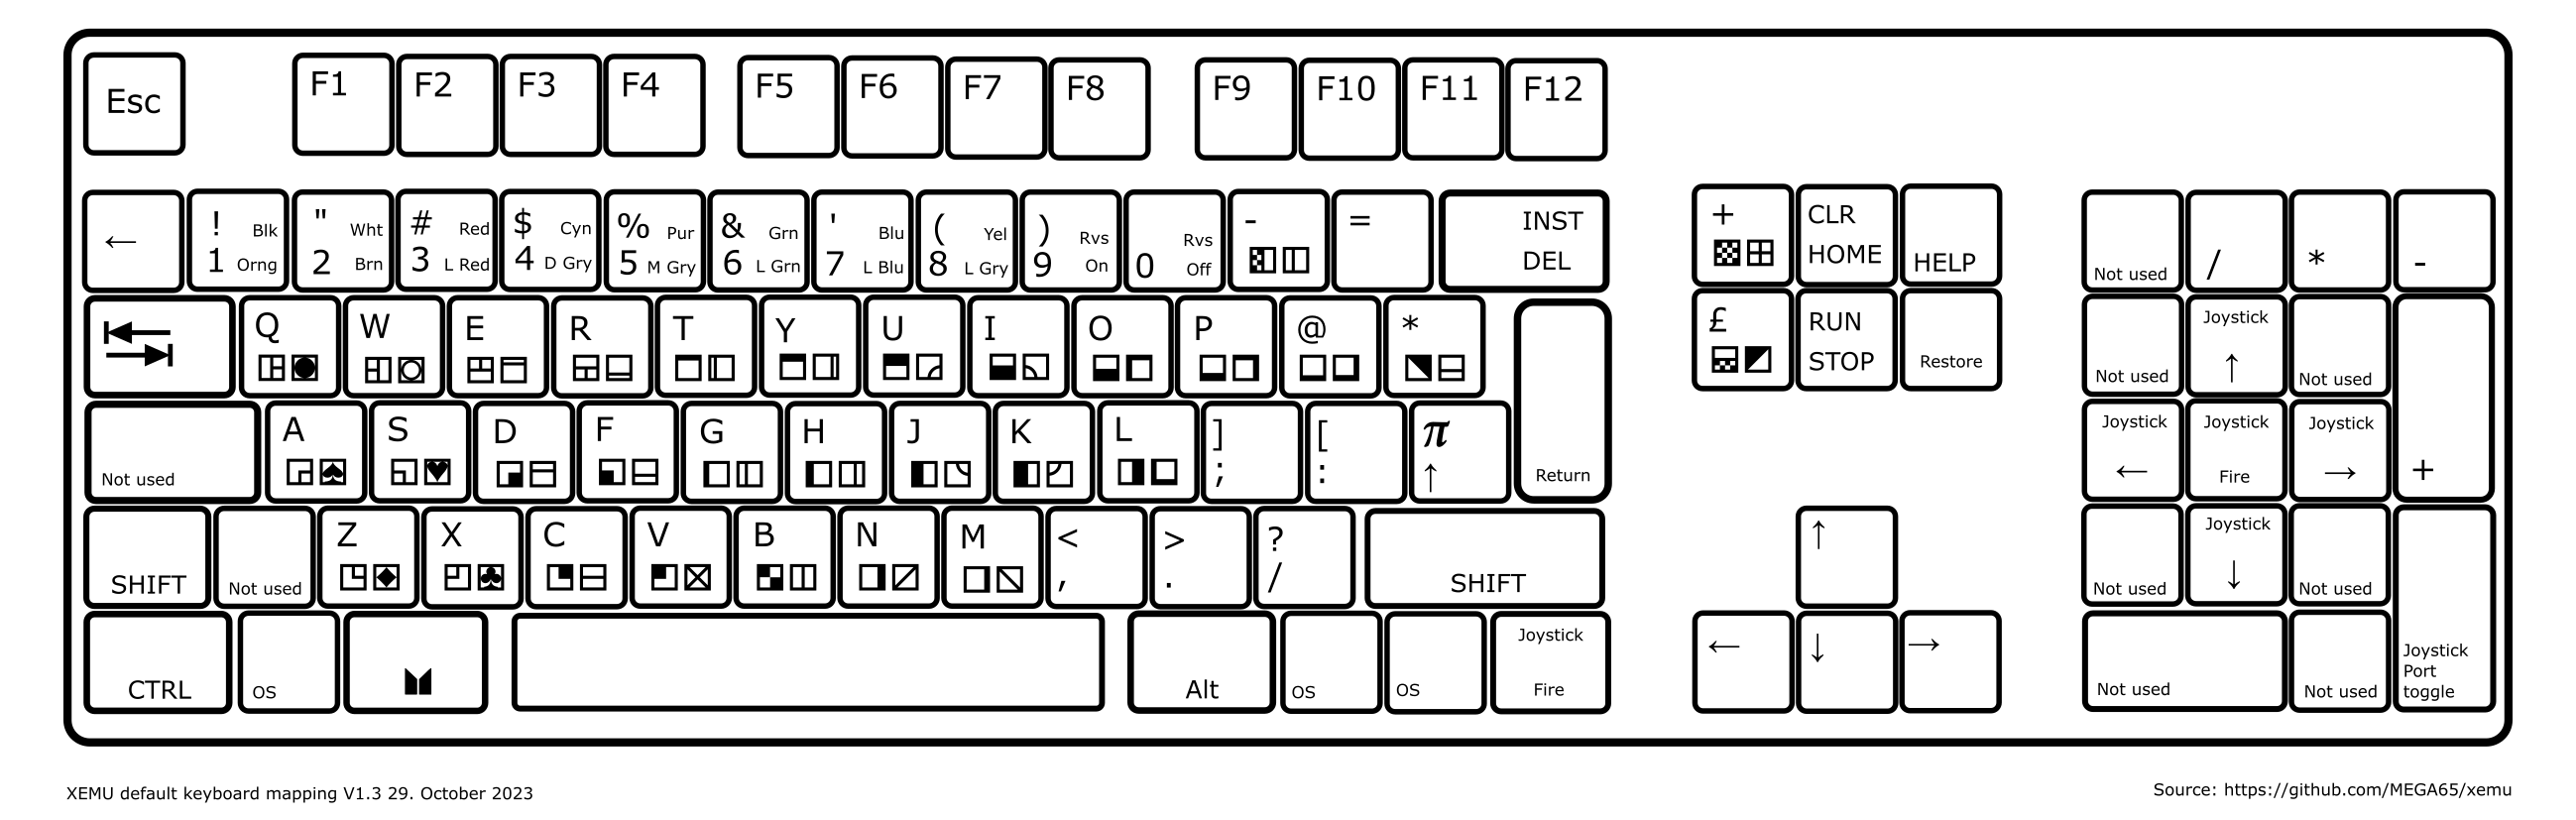
\includegraphics[width=\linewidth]{images/xemu-extended-keyboard.png}
\end{center}

Op de meeste pc-toetsenborden staan \specialkey{RUN\\STOP} en \widekey{RESTORE} naast elkaar,
zodat deze toetscombinatie eenvoudig is in te voeren.

Deze afbeelding toont de PETSCII-glyphen zoals ze op een MEGA65-toetsenbord verschijnen, met de
\megasymbolkey-glyphe links en de \specialkey{Shift}-glyphe rechts. Merk op
dat op een pc-toetsenbord de toets voor \megasymbolkey rechts van de
\specialkey{Shift} staat.

Xemu biedt twee joysticks (een per keer) op het numerieke toetsenbord.
\specialkey{Enter} op het numerieke toetsenbord wordt gebruikt om bij herhaaldelijk drukken poorten 1 en 2 in en uit te schakelen.

Wees u ervan bewust dat de emulator standaard \megakey{F9} \megakey{F10}
\megakey{F11} als eigen sneltoetsen heeft gedefinieerd. Als u deze toetsen wilt gebruiken met de
geëmulieerde MEGA65, moet u de toetsenbordindeling aanpassen. De bestanden staan in de
map met de Xemu-instellingen zoals uitgelegd op bladzijde
\pageref{sec:sdcard-settings-location}. Dit doet u door
\stw{keymap-default.cfg} te kopiëren naar \stw{keymap.cfg} en vervolgens de volgende regels te verwijderen:

\begin{tcolorbox}[colback=black,coltext=white]
\verbatimfont{\codefont}
\begin{verbatim}
XEMU-EXIT F9
XEMU-FULLSCREEN F11
\end{verbatim}
\end{tcolorbox}

en te wijzigen in:

\begin{tcolorbox}[colback=black,coltext=white]
\verbatimfont{\codefont}
\begin{verbatim}
F9 Unknown
F11 Unknown
\end{verbatim}
\end{tcolorbox}

naar:

\begin{tcolorbox}[colback=black,coltext=white]
\verbatimfont{\codefont}
\begin{verbatim}
F9 F9
F11 F11
\end{verbatim}
\end{tcolorbox}

Nadat deze toetsen opnieuw zijn toegewezen, zijn de functies voor volledig scherm en afsluiten nog steeds beschikbaar via
het menu. Klik met rechts (of Ctrl-klik) ergens in het venster om dit te openen.

\subsection{Problemen met starten op Apple MacOS}

Als het bericht \stw{macOS cannot verify that this app is free from malware} verschijnt,
gebruik dan de volgende procedure wanneer u de app voor de eerste keer opent:\index{Apple}
\index{macOS}

\begin{itemize}
  \item Open Finder op uw Mac.
  \item Ctrl-klik (of rechtsklik) op het Xmega65-app-pictogram.
  \item Selecteer in het contextmenu \stw{Open}.
  \item Het bericht verschijnt opnieuw, maar deze keer is er een knop \stw{Open}.
        Klik op \stw{Open}. U hoeft deze procedure slechts de eerste keer uit te voeren.
		Vanaf nu kunt u de app normaal openen.
\end{itemize}

\subsection{Instellingen bijwerken}
\label{sec:sdcard-settings-location}
\index{SD-kaart}

U kunt het Xemu-instellingsbestand bewerken om de toetsenbordindeling aan te passen of een
reservekopie van het SD-kaart-imagebestand te maken. Open vanuit Xemu het menu om deze bestanden te openen: selecteer
menu, selecteer \stw{Debug / Advanced} en vervolgens \stw{Browse system folder}. Bewerk de
bestanden \stw{keymap-default.cfg} en \stw{mega65-default.cfg} met een teksteditor.
Voor specifieke instructies over het wijzigen van \stw{keymap-default.cfg} verwijzen we naar
bladzijde \pageref{sec:xemu-keyboard}.

\begin{center}
  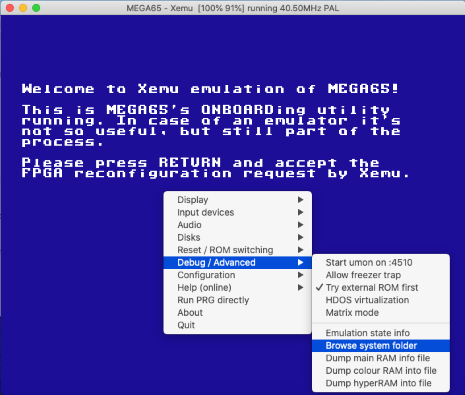
\includegraphics[width=0.5\linewidth]{images/xemusettings.png}
\end{center}

De locatie van de Xemu-systeemmap verschilt per besturingssysteem:

\begin{itemize}
    \item Windows (kan in de adresbalk van de verkenner worden gekopieerd):
    \stw{\%appdata\%$\textbackslash$xemu-lgb$\textbackslash$mega65}
    \item Linux:
    \stw{$\textasciitilde$/.xemu-lgb/}
    \item Macintosh:
    \stw{$\textasciitilde$/Library/Application$\textbackslash$ Support/xemu-lgb/mega65/}
\end{itemize}

\section{De Live ISO-image gebruiken}
\label{sec:live-iso-image}

De Live ISO-image is het product van een vrijwillige gemeenschap; niet van het MEGA65-team. We nemen deze op voor uw gemak.

\subsection{Een opstartbare USB-stick of DVD maken}

Er zijn veel manieren om een live ISO-image te maken. De methode die u kiest hangt af van uw besturingssysteem en of u deze op een USB-station wilt installeren of op een DVD wilt branden. Het branden op een DVD is eenvoudig, ervan uitgaande dat u een computer met een DVD-brander hebt. Als u een sneller opstartbaar USB-station wilt maken, probeert u een van de onderstaande methoden:

Als u Windows gebruikt, overweeg dan een hulpprogramma zoals \url{http://www.isotousb.com/}.

Op Linux kunt u de instructies op \url{https://fossbytes.com/create-bootable-usb-media-from-iso-ubuntu/} volgen.

Voor Apple Macs zijn de instructies op
\url{https://ubuntu.com/tutorials/create-a-usb-stick-on-macos#1-overview} beschikbaar.

Vergelijkbare instructies zijn beschikbaar voor andere populaire computers, zoals Amiga's (\url{https://forum.hyperion-entertainment.com/viewtopic.php?t=3857}) of Sun UltraSPARC-werkstations (\url{https://forums.servethehome.com/index.php?threads/how-to-create-a-bootable-solaris-11-usb.1998/}).

Tot slot is de populaire, eenvoudig te gebruiken en gratis cross-platform belanaEtcher beschikbaar op \url{https://www.balena.io/etcher/}.

\subsection{Aan de slag}

Om potentiële auteursrechtelijke kwesties te vermijden, bevat de opstartbare ISO-image geen propriëtaire ROM's voor de MEGA65, zoals oude C65-ROM's. Het bevat wel een vervangende open-source-ROM van ons OpenROMs-project.\index{OpenROMs} Deze ROM start op in een BASIC 2-omgeving waarmee u veel C64-programma's kunt laden en uitvoeren, zoals te zien is in de onderstaande afbeelding:

\screenshotwrap{images/liveiso-openrom.png}

Als u een C65-ROM met BASIC 10 wilt gebruiken, download het juiste ROM-bestand en plaats het op een andere USB-stick met de naam \stw{MEGA65.ROM}. Bij het opstarten zal de MEGA65 vragen of een ROM is gedownload; zoals te zien is in de onderstaande afbeelding:

\screenshotwrap{images/liveiso-rom-usb-prompt.png}

Als de Live ISO geen ROM kan vinden, zal het u vragen om een ROM te downloaden; zoals hieronder te zien is:

\screenshotwrap{images/liveiso-rom-download-prompt.png}

\subsection{Andere functies van de Live ISO}

Zoals de bovenstaande schermafbeeldingen laten zien, biedt de Live ISO diverse handige bureaubladkortingen. Aan de linkerzijde staan koppelingen om de
MEGA65-emulator en de C65-emulator te starten, zodat u kunt testen of programma's
op beide platforms werken. Zoals eerder vermeld zijn beide emulators in ontwikkeling en mogelijk niet 100\% compatibel.

Een andere koppeling geeft toegang tot het grote Mega65-boek. Deze omvattende band van
ongeveer 800 pagina's bevat de officiële MEGA65-documentatie. Het grootste deel van deze handleiding voor ontwikkelaars is ook opgenomen in het grote Mega65-boek.

Deze ISO bevat ook documentatie voor de C65 Notepad; een programma voor de C65 en MEGA65 geschreven door Snoopy (de ontwikkelaar van de Live ISO-image). Een ``lees mij''-bestand bevat verdere informatie over de Live ISO.

Tot slot zijn er aan de rechterzijde koppelingen om een C65-ROM te downloaden en het grote Mega65-boek bij te werken naar de nieuwste versie. Hiermee voorkomt u dat u steeds een nieuwe opstartbare image moet maken wanneer er een frequente update van het grote Mega65-boek wordt uitgebracht.

De volledige inhoud van de Live ISO-image is toegankelijk via de bestandsverkenner.

% 2022-11-28 edits by nobruinfo
% 2021-03-17 edits by SBC

\chapter{Gegevensoverdracht en foutopsporing}
\label{cha:transfer-and-debug-tools}

De sleutel tot effectieve cross-platform-ontwikkeling is het hebben van snelle en
eenvoudige middelen om programmatuur op de MEGA65 te testen. Dit
geldt zeker nu de MEGA65-emulator nog in ontwikkeling is.
Zelfs wanneer de MEGA65-emulator voltooid is, zal het onwaarschijnlijk
zijn dat deze volledige compatibiliteit op volledige snelheid kan bieden,
omdat de MEGA65 veel veeleisender is om te emuleren dan de C64.

Er zijn verschillende hulpprogramma's die kunnen worden gebruikt voor gegevensoverdracht en
foute opsporing. Deze maken doorgaans gebruik van ofwel de seriële
monitorinterface van de MEGA65, of via de fast-ethernetadapter van de MEGA65. De
seriële monitorinterface is beschikbaar via de UART-lijnen op de JB1-
connector.

Als u geen toegang hebt tot de seriële monitorinterface, worden er
hulpprogramma's ontwikkeld voor de fast-ethernetpoort die een deel,
maar niet alles, van de mogelijkheden van de seriële monitor
bieden. Deze worden gedocumenteerd zodra ze beschikbaar zijn. Het
restant van dit hoofdstuk richt zich op methoden die de seriële
monitorinterface gebruiken.

U kunt een 3.3V UART-adapter op de juiste
lijnen aansluiten, of gemakkelijker, een TE-0790-03 JTAG-debugmodule
op deze connector plaatsen. Dit geeft u een USB-verbinding die kan worden gebruikt
voor het overzetten van software, op afstand fouten opsporen en geheugen inspecteren, alsmede
het activeren of flashen van bitstreams. Met deze verbinding
zijn de volgende hulpprogramma's beschikbaar:

\section{m65-hulpprogramma}

Het repository \url{https://github.com/mega65/mega65-tools} bevat een
aantal hulpprogramma's, utilities en voorbeeldprogramma's. Deze hulpprogramma's zijn voornamelijk voor Linux maar kunnen worden gebruikt op Windows met Cygwin. Een van die hulpprogramma's is
het \stw{m65}-hulpprogramma. Dit is eigenlijk een zakmes
verzameling van utilities in één. Veelgebruikte functies
zijn onder meer:

\subsection{Schermfoto's met het m65-hulpprogramma}

Om een schermfoto van de MEGA65 te maken:

\begin{screencode}
m65 -S
\end{screencode}

Dit maakt een bestand aan met de naam \stw{mega65-screen-000000.png},
of als dit bestand al bestaat, wordt het eerste niet-gebruikte nummer gebruikt
in plaats van \stw{000000}.

Merk op dat deze schermfotofunctie werkt door \stw{m65} de
functionaliteit van de VIC-IV te laten emuleren. Hoewel het uitstekende digitale schermfoto's oplevert, komt het mogelijk niet exact overeen met het werkelijke scherm van de
MEGA65. Op het moment van schrijven rendert het geen sprites of bitplanelen, alleen tekst- en bitmap-gebaseerde videomodi.

\subsection{Een programma laden en uitvoeren op de MEGA65}

Om een programma op de MEGA65 te laden en uit te voeren, kunt u een commando als het volgende gebruiken:

\begin{screencode}
m65 -F -4 -r foo.prg
\end{screencode}

De optie \stw{-F} draagt \stw{m65} op de MEGA65 te herstarten
voordat het programma wordt geladen.

De optie \stw{-4} draagt \stw{m65} op de MEGA65
naar C64-modus te schakelen voordat het programma wordt geladen. Als dit wordt weggelaten,
zal het proberen het programma in C65-modus te laden.

De optie \stw{-r} draagt \stw{m65} op het programma onmiddellijk
na het laden uit te voeren.

Merk op dat dit commando werkt met het normale BASIC LOAD-commando en
daarom beperkt is tot het laden van programma's in het onderste 64 KB van het geheugen.

\subsection{De FPGA herconfigureren om een andere bitstream uit te voeren}

Om een andere MEGA65-bitstream uit te proberen, kan een commando als het volgende worden
gebruikt:

\begin{screencode}
m65 -b bitstream.bit
\end{screencode}

Dit zal de genoemde bitstream naar de FPGA zenden. Omdat de
FPGA door deze actie wordt herconfigureerd, zal het momenteel
uitgevoerde programma niet alleen worden gestopt, maar ook het hoofdgeheugen zal worden
gewist. Voor modellen van de MEGA65 die zijn uitgerust met 8 MB of 16 MB
uitbreidingsgeheugen, worden deze uitbreidingsgeheugens geïmplementeerd in externe
chips en dus zullen de inhoud daarvan niet worden gewist.

Voor niet-MEGA65-bitstreams (zoals zxunomega65 en gbc4mega65), gebruik in plaats daarvan het argument '-q':

\begin{screencode}
m65 -q bitstream.bit
\end{screencode}

\subsection{Toetsenbordinvoer op afstand}

De toetsenbordinterface van de MEGA65 ondersteunt het overzetten van
synthetische toetsgebeurtenissen via de registers \$D615 -- \$D617.
Het \stw{m65}-hulpprogramma gebruikt dit om typen op afstand op de MEGA65
mogelijk te maken op een manier die transparant is voor software. Er zijn drie manieren om dit
te gebruiken:

\begin{screencode}
m65 -t ditiswattekst
\end{screencode}

Deze vorm typt de opgegeven tekst, in dit geval {\em ditiswattekst}, maar
simuleert niet het indrukken van \specialkey{RETURN}. Als u
het indrukken van \specialkey{RETURN} wilt simuleren, gebruikt u \stw{-T}
in plaats van \stw{-t}, bijvoorbeeld:

\begin{screencode}
m65 -T list
\end{screencode}

Dit zou het LIST-commando typen en uitvoeren.

Tot slot is het mogelijk om algemene toetsenbordbesturing op afstand te starten via:

\begin{screencode}
m65 -t -
\end{screencode}

In deze modus wordt elke toets, die op het toetsenbord van de computer
waarop \stw{m65} draait, doorgegeven aan de MEGA65. Merk op dat
niet alle speciale toetsen worden ondersteund en dat er enige vertraging is, dus
het gebruik van de toetsherhalingsfunctie kan onverwachte resultaten opleveren. Voor besturing op afstand in het algemeen is het echter een zeer nuttige voorziening.

\subsection{Unit-testing en logboekondersteuning}

Het \stw{m65}-hulpprogramma ondersteunt unit-testing
direct op MEGA65-hardware. Wanneer de \textit{unit testing-modus} actief is,
wacht \stw{m65} tot de MEGA65 bepaalde byte-reeksen via de
seriële interface stuurt die de huidige status (gestart, geslaagd, mislukt) signaleren
van een gegeven test. Daarnaast is het mogelijk om logboekberichten te verzenden vanaf
de MEGA65 naar de hostcomputer.

De unittestingmodus wordt betreden door \stw{m65} aan te roepen met de vlag \stw{-u}.
Om een BASIC-programma op afstand in C65-modus uit te voeren en tegelijk \stw{m65}
in de \textit{unittestingmodus} te zetten, kan het volgende commando worden gebruikt:

\begin{screencode}
    m65 -Fur attic-ram.prg -w tests.log
\end{screencode}

De opties \stw{-F} en \stw{-r} vertellen \stw{m65} om de MEGA65 te herstarten
voordat het programma "attic-ram.prg" wordt geladen en automatisch uitgevoerd.
De optie \stw{-u} vertelt \stw{m65} vervolgens om in de \textit{unittestingmodus} te gaan
in plaats van te stoppen na het starten van het programma.
De optionele optie \stw{-w} zorgt ervoor dat \stw{m65} de testresultaten aan het
bestand "test.log" toevoegt (het bestand aanmaakt als het nog niet bestaat).

Merk op dat \stw{m65} automatisch de \textit{unittestingmodus} verlaat
als er gedurende meer dan 10 seconden geen teststatussignalen zijn ontvangen.

Er is ondersteuning voor het verzenden van unittestingsignalen naar de hostcomputer vanuit
C- en BASIC 65-programma's:

\subsubsection{Unit-tests gebruiken met C}

De MEGA65 libc bevat ondersteuning voor unit-testing via functies gedefinieerd in
\stw{tests.h} en \stw{tests.c}.

Om het begin van een test te signaleren, includeert u \stw{tests.h} en gebruikt u:

\begin{verbatim}
    unit_test_setup("testName",issueNumber);
\end{verbatim}

waarbij \textit{"testName"} een leesbare naam van de test is (bijvoorbeeld
"VIC-II") en \textit{issueNumber} een verwijzing naar het bijbehorende
bug-issue (bijvoorbeeld het issue-nummer van GitHub).

Na het starten van een test kunnen geslaagde tests worden gesignaleerd met
de functie unit\_test\_ok():

\begin{verbatim}
    unit_test_ok();
\end{verbatim}

Een mislukte test wordt gesignaleerd met unit\_test\_fail():

\begin{verbatim}
    unit_test_fail("fail message");
\end{verbatim}

Elke keer dat de functies unit\_test\_ok() of unit\_test\_fail()
worden aangeroepen, wordt het \textit{sub-issue} van de test (gerapporteerd op de
hostcomputer) verhoogd. Dit maakt het eenvoudiger om meerdere tests in één bestand te combineren en
te identificeren.

U kunt willekeurige logboekberichten verzenden via unit\_test\_log():

\begin{verbatim}
    unit_test_log("hello world from mega65!");
\end{verbatim}

...en ten slotte, wanneer alles klaar is, wordt het einde van unit-testing gesignaleerd
door het gebruik van:

\begin{verbatim}
    unit_test_done();
\end{verbatim}


\subsubsection{Unit-tests gebruiken met BASIC 65}

\stw{b65support.bin} is een machinetaalmodule die ondersteuning biedt voor
unit-testing vanuit BASIC 65. Deze staat in het mega65-tools-
repository op \url{https://github.com/MEGA65/mega65-tools} en kan worden gebouwd met:

\begin{verbatim}
    make bin65/b65support.bin
\end{verbatim}

Het bestand \stw{b65support.bin} is dan beschikbaar in de map \stw{bin65}.

Deze module werkt door de USR-vector om te leiden om de functies
uit te voeren die nodig zijn om te communiceren met de test-host.

In een geautomatiseerd testsenario wilt u mogelijk het binaire bestand \stw{b65support.bin}
overzetten naar het MEGA65-geheugen door middel van \stw{m65}:

    \begin{screencode}
        m65 -@ mega65-tools/bin65/b65support.bin@15fe
    \end{screencode}


Het is natuurlijk ook mogelijk om \stw{b65support.bin} rechtstreeks vanaf de
MEGA65 te laden door de \stw{M65UTILS.D81}-image van de Freezer te koppelen en het volgende commando te geven:

\begin{screencode}
    BLOAD "B65SUPPORT.BIN"
\end{screencode}

Na het laden wordt \stw{b65support.bin} geïnitialiseerd met:

\begin{screencode}
    SYS $1600
\end{screencode}

Na initialisatie biedt \stw{b65support.bin} de volgende functies:

\begin{screencode}
    A=USR(<issueNum>)
\end{screencode}
bereidt een nieuwe test voor met nummer <issueNum> en herstelt het subissue-nummer naar 0.

\begin{screencode}
    A=USR("=<testName>")
\end{screencode}
stelt de testnaam in en stuurt het testsignaal; bijvoorbeeld: \stw{A=USR("=VIC-III")}
stelt de testnaam in op 'VIC-III' en signaleert de hostcomputer dat de test
is gestart.

\begin{screencode}
    A=USR("/<logMessage>)
\end{screencode}
stuurt een logboekbericht naar de hostcomputer.

\begin{screencode}
    A=USR("P")
\end{screencode}
stuurt het signaal 'geslaagd' naar de hostcomputer en verhoogt het subissue-nummer.

\begin{screencode}
    A=USR("F")
\end{screencode}
stuurt het signaal 'test mislukt' naar de hostcomputer en verhoogt
het subissue-nummer.

\begin{screencode}
    A=USR("D")
\end{screencode}
stuurt het signaal 'test voltooid' naar de hostcomputer.

Alle aanroepen retourneren het huidige subissue-nummer of \stw{?ILLEGAL QUANTITY ERROR} in
geval van een ongeldig commando.

\subsubsection{BASIC 65-voorbeeld}

Het volgende is een volledig BASIC 65-voorbeeld dat laat zien hoe de
unittestingfuncties van \stw{m65} worden gebruikt:

\begin{screencode}
    100 rem attic ram cache test
    110 poke $bfffff2,$e0         : rem schakel cache van zolder-ram in
    120 sys $1600                 : rem initialiseer testmodule
    130 a=usr(379)                : rem zet issue-nummer
    140 a=usr("=attic-ram-cache") : rem zet testnaam
    150 bank128:poke0,65          : rem uit voorzorg
    160 b0=$8000000 : b1=$8000100 : rem zolden-ram-gebieden om te testen
    170 for r=0 to $ff
    180   poke b0+r,0             : rem vul gebied 1 met 0
    190   poke b1+r,$ff           : rem vul gebied 2 met $ff
    200 next r
    210 for t=1 to 10             : rem 10 pogingen
    220   poke b0,32              : rem schrijf naar b0
    230   for x=0 to $ff:t1=b1+x
    240     a=peek(b0)            : rem lees uit b0
    250     b=peek(t1):b=peek(t1) : rem lees tweemaal uit t1
    260     ifb<>255 thenf=t:t=11:x=256   : rem dit mag niet gebeuren
    270   next x
    280 next t
    290 if f=0 then begin
    300   print "geen fouten gevonden na";t;"pogingen."
    310   a=usr("p")              : rem signal 'test passed' to host
    320 bend : else begin
    330   a=usr("f")              : rem signal 'test failed' to host
    340   print "hyper-ram-fout gedetecteerd na";f;"pogingen."
    350   print "peek($";hex$(t1);") [t1] is";b;"maar moet 255 zijn"
    360 bend
    370 a=usr("d")                : rem test gereed    
\end{screencode}

\section{M65Connect}

Dit is een cross-platform grafisch hulpprogramma dat beschikbaar is voor Windows, Linux
en MacOSX, waarmee toegang wordt geboden tot de meeste functies van
het \stw{m65}-hulpprogramma, zonder dat een
commandoregel nodig is, of zonder dat u het hulpprogramma voor uw favoriete
besturingssysteem hoeft te compileren.

Het repository voor M65Connect is: \url{https://github.com/MEGA65/m65connect}

De nieuwste binaire versie is beschikbaar op \url{https://files.mega65.org}.

Met de MEGA65 of Nexys FPGA uitgeschakeld, sluit een USB-kabel aan van uw computer op de MEGA65 of Nexys FPGA-board. Voer het \textit{M65Connect}-programma uit en volg de aanwijzingen om verbinding te maken. Het programma helpt u bij het identificeren van welke USB Serial Port moet worden gebruikt.

Met dit hulpprogramma kunt u eenvoudig PRG-programma's en diverse andere bestanden overdragen. M65Connect kan de overdracht, het schakelen naar C64-modus en de uitvoering van programma's afhandelen.

\section{mega65\_ftp}

Het \stw{mega65}\_\stw{ftp}-hulpprogramma van
het repository \url{https://github.com/mega65/mega65-tools} is
enigszins misleidend genoemd: hoewel het
een File Transfer Program is, gebruikt het niet het File Transfer
Protocol (FTP). Het gebruikt in plaats daarvan de seriële monitorinterface om
de MEGA65 op afstand te besturen en heeft directe toegang tot de SD-kaart om het
kopiëren van bestanden tussen de MEGA65 en de hostcomputer mogelijk te maken.

Merk op dat het de staat van de MEGA65 niet perfect herstelt bij het afsluiten,
en dus alleen moet worden gebruikt wanneer de MEGA65 bij de READY.-prompt staat,
zodat eventuele draaiende software niet in de war raakt. Met name moet u
het gebruik vermijden wanneer een gevoelig programma draait, zoals
het Freeze-menu, het MEGA65-configuratiehulpprogramma of het MEGA65
Format/FDISK-hulpprogramma. (Dit probleem kan met weinig
inspanning worden opgelost, als iemand de tijd en interesse heeft om het te fixen).

Bij uitvoering biedt het een FTP-achtige interface die de
commando's \stw{get}, \stw{put}, \stw{rename} en \stw{dir} ondersteunt.
Merk op dat u bij het plaatsen van een bestand moet zorgen dat het een
naam heeft die volledig in hoofdletters staat en een DOS-compatibele 8.3-teken
bestandsnaam heeft. Dit komt door beperkingen in zowel \stw{mega65}\_\stw{ftp} als de
VFAT32-bestandssysteemcode van de Hypervisor van de MEGA65. Opnieuw kunnen deze problemen
worden opgelost met een bescheiden hoeveelheid inspanning van de kant van een
gemotiveerd lid van de gemeenschap.

Tot slot is het programma \stw{mega65}\_\stw{ftp} {\em zeer} langzaam bij het pushen
van nieuwe bestanden naar de MEGA65, met doorgaans snelheden van rond de 5 KB/sec.
Dit komt deels doordat de seriële interface in staat is om
gegevens over te dragen met slechts 40 KB/sec (bij 4.000.000 bits per
seconde), en deels doordat het besturingsproces op afstand resulteert in
veel heen-en-weerverkeer waarbij hulpoutines op de MEGA65 worden uitgevoerd om
sectoren op de SD-kaart te lezen, schrijven en verifiëren. Het zou heel
haalbaar zijn om dit te verbeteren tot bijna 40 KB/sec, en mogelijk
sneller met een combinatie van gegevenscompressie,
deduplicatie van identieke sectoren (met name bij het uploaden van schijf-
images) en andere technieken. Opnieuw zou dit een zeer welkome bijdrage zijn die iemand uit de gemeenschap zou kunnen leveren
ten algemene nutte.

\section{TFTP-server}

Er is een echte TFTP-server voor de MEGA65 in ontwikkeling die snelle
TFTP-overdrachten via de 100 Mbit-ethernet ondersteunt en die kan worden gebruikt om
zeer snel bestanden van de MEGA65 te lezen. Snelheden van bijna 1 MB/sec
zijn mogelijk, afhankelijk van de prestaties van de SD-kaart. In plaats van
DHCP te gebruiken, zal dit hulpprogramma reageren op {\em elk} IP-adres dat eindigt op
.65. Het gebruikt altijd het MAC-adres 40:40:40:40:40:40. Echte DHCP-
ondersteuning en het gebruik van het geconfigureerde ethernet-MAC-adres van de MEGA65
worden mogelijk in de toekomst toegevoegd.

Belangrijker nog, de ondersteuning voor het schrijven van
bestanden naar de SD-kaart is nog niet volledig en wordt geblokkeerd door de behoefte
aan de implementatie van de nodige functies in de Hypervisor van de MEGA65 voor het aanmaken en
vergrootten van bestanden. Een bijzondere uitdaging is het mogelijk maken van het aanmaken van
bestanden met aaneengesloten clusters zoals vereist voor D81-schijfimages: als
een D81-bestand gefragmenteerd is, kan het niet worden gekoppeld, omdat het
koppelingsmechanisme een pointer naar het aaneengesloten blok van de
SD-kaart vereist dat de schijfimage bevat.
In de tussentijd kan \stw{mega65}\_\stw{ftp} als alternatief worden gebruikt.

\section{Een BASIC-tekstbestandlisting omzetten naar een PRG-bestand}

Als u een ongetokeniseerd BASIC-programma in platte-tekstformaat hebt dat afkomstig is van bijvoorbeeld een internetbericht, en u wilt het op de MEGA65 proberen zonder het in te typen, dan is het mogelijk het om te zetten naar een PRG.

\textit{C64List} is een Windows-gebaseerd commandoregelhulpprogramma waarmee u de conversie kunt uitvoeren. Zodra u een \textit{.PRG}-bestand hebt, kunt u een hulpprogramma zoals M65Connect gebruiken om het naar de MEGA65 of Nexys FPGA te uploaden.

C64List is beschikbaar voor download op \url{http://www.commodoreserver.com/Downloads.asp}

Zorg ervoor dat u een programmalijst in een bestand op uw lokale computer hebt opgeslagen (bijvoorbeeld \textit{program.txt}) gecodeerd als ANSI of UTF8.

Gebruik C64List om het bestand om te zetten naar een PRG-bestand:
    
\begin{tcolorbox}[colback=black,coltext=white]
    \begin{verbatim}
        C64List program.txt -prg
    \end{verbatim}
\end{tcolorbox}

Nu kunt u uw nieuw geconverteerde programma uploaden naar de MEGA65 met M65Connect of een van de eerder beschreven hulpprogramma's.

Het is vermeldenswaard dat deze methode niet 100\% effectief zal zijn bij listings met speciale PETSCII-tekens. Programma's met PETSCII vereisen enige bewerking op de MEGA65 zelf voordat ze op schijf worden opgeslagen.

\chapter{Assemblers}

Onderstaande tabel geeft een overzicht van assemblers waarvan bekend is dat ze met de MEGA65 werken.
Voor algemeen gebruik raden we {\bf ACME} aan, omdat het goede ondersteuning biedt voor de
45GS02-instructieset, open source is en bovendien in C is geschreven. Dat laatste
betekent dat de assembler op termijn naar de MEGA65 geporteerd zou kunnen worden om er native te draaien.

\begin{longtable}{ | l | l | l | l |}\hline
Naam     & 45GS02 & Bron & Verwijzing \\\hline
ACME     &  ja    & C    & \url{https://sourceforge.net/projects/acme-crossass}\\
KickAss  &  ja    & Java & \href{https://gitlab.com/jespergravgaard/kickassembler65ce02}{gitlab.com/jespergravgaard/kickassembler65ce02}\\
LLVM-MOS &  ja    & C++  & \url{https://llvm-mos.org/wiki/Welcome}\\
Ophis    &  ja    & Python & \url{https://github.com/michaelcmartin/Ophis}\\
BSA      &  ja    & C    & \url{https://github.com/Edilbert/BSA}\\
CA65     &  nee\footnote{Onze fork van CA65 (onderdeel van CC65) herkent de CPU van de MEGA65 correct, maar heeft geen expliciete ondersteuning voor de mogelijkheden van de processor} & C & \url{https://github.com/mega65/cc65}\\\hline
\end{longtable}

De {\bf BSA}-assembler wordt momenteel gebruikt om de {\bf MEGA65.ROM} te bouwen.
Het grootste deel van de broncode is geschreven in de syntaxis van de oude
{\bf BSO}-assembler (Boston Systems Office), die in de jaren 1989--1991 werd
gebruikt door softwareontwikkelaars aan de C65. De {\bf BSA}-assembler heeft een
compatibiliteitsmodus waarmee deze oude broncodes met weinig of geen aanpassingen
kunnen worden geassembleerd. De {\bf BSA}-assembler bevat momenteel alleen een
beschrijving van de commando's in de C-broncode van de assembler.

Het {\bf LLVM-MOS}-project wordt geleverd met een GNU-compatibele macro-assembler
en -disassembler die alle mnemonieken van de 45GS02 ondersteunt. Het kan als
zelfstandig hulpprogramma worden gebruikt met het commando {\bf llvm-mc}.

\chapter{C- en C-achtige compilers}

Kort antwoord: CC65 en KickC werken beide op de MEGA65.

Zowel CC65 als KickC werken op de MEGA65, maar beide hebben standaard
alleen een C64-geheugenmodel en gebruiken uitsluitend 6502-opcodes.
Het zou geweldig zijn als iemand een C65-geheugenconfiguratie voor
CC65 zou ontwikkelen; dat zou niet al te moeilijk moeten zijn.

CC65 ondersteunt overlays, wat krachtig kan worden ingezet met het
extra geheugen van de MEGA65 om programma's groter dan 64 KB mogelijk
te maken. Daarvoor is echter een geschikte loader nodig, die nog niet
bestaat.

Op dezelfde manier zou het aanpassen van de codegenerator van CC65 om
45GS02-mogelijkheden te gebruiken niet bijzonder moeilijk zijn en zou
het helpen om de anders vreselijk trage en omvangrijke code die CC65
produceert te overwinnen. Het toevoegen van volledige ondersteuning
voor de 45GS02-CPU-mogelijkheden in CA65 (of nog beter: het laten
produceren van ACME-compatibele assembleeruitvoer door CC65) zou van
overweldigend voordeel zijn en niet bijzonder moeilijk te realiseren.
Dit zouden allemaal geweldige taken zijn om mee bezig te zijn terwijl
u wacht op uw MEGA65 DevKit!

Een voorbeeldsjabloon voor een C-programma dat met CC65 kan worden
gecompileerd en op de MEGA65 kan worden uitgevoerd, staat in het
repository \url{https://github.com/MEGA65/hello-world}. Dit repository
kan zelfs CC65 downloaden en compileren als u dat nog niet op uw
systeem hebt geïnstalleerd. Het repository werkt op Linux en Mac en op Windows via het Windows Subsystem for Linux (WSL).

Het LLVM-MOS-project (\url{https://llvm-mos.org}) heeft een
MEGA65-doelplatform dat is getest met C99, C++11 en Rust. De LLVM
MOS-compiler heeft ondersteuning voor 45GS02-instructies
(\texttt{-mcpu=mos45gs02}) en wordt geleverd met een assembler en
disassembler. Voorgecompileerde binaire bestanden van de SDK zijn
beschikbaar voor Linux, Windows en macOS.

\section{MEGA65 libc}

Er wordt een C-bibliotheek ontwikkeld voor de MEGA65, die al een
aantal nuttige functies bevat. Deze bibliotheek is beschikbaar via
\url{http://github.com/mega65/mega65-libc}. De procedures, functies
en definities die het biedt, zijn gedocumenteerd in een apart
hoofdstuk.

De MEGA65 libc is momenteel alleen beschikbaar voor LLVM en CC65,
hoewel we een KickC-port hiervan zeer op prijs zouden stellen.

\chapter{MEGA65 Standard C Library}

Er wordt een C-bibliotheek ontwikkeld voor de MEGA65, die al een
aantal nuttige functies bevat. Deze bibliotheek is beschikbaar via
\url{http://github.com/mega65/mega65-libc}. De procedures,
functies en definities die zij biedt, worden gedocumenteerd in een apart
hoofdstuk.

\section{Structuur en gebruik}

De MEGA65-libc wordt bewust alleen als broncode aangeboden, met
functiegroepen in aparte bestanden en afzonderlijke headerbestanden voor
inclusie. Het idee is dat u alleen de headerbestanden opneemt die u nodig
heeft, en alleen de benodigde bronbestanden toevoegt aan de lijst van
bronbestanden van het programma dat u compileert. Daarmee voorkomt u dat
de compiler functies in uw gecompileerde programma opneemt die nooit
worden gebruikt, waardoor kostbaar geheugen verspild wordt.

Let op dat sommige bronbestanden van de bibliotheek in C geschreven zijn
en dus bestanden met de extensie \stw{.c} betreffen, terwijl andere in
assemblerertaal geschreven zijn, hetzij vanwege efficiëntie, hetzij uit
noodzaak, en de extensie \stw{.s} hebben.

Gangbaar gebruik is de broncode van mega65-libc uit te checken in een
naburige map of binnen de bronmap van uw eigen project. In het laatste
geval kan dit met behulp van de git submodule-faciliteit.

De volgende secties documenteren elk van de headerbestanden en de
bijbehorende functies die zij bieden.

\section{conio.h}

\titleformat*{\subsection}{\normalfont\huge\bfseries\color{blue}}


\subsection{conionit}
\index{conionit}
\begin{description}[leftmargin=2.4cm,style=nextline]
\item [Beschrijving:] {Initialiseert de interne status van de bibliotheek}\item [Syntaxis:] \stw{void conioinit(void)}\item [Opmerkingen:] {U moet deze functie aanroepen voordat u een conio-bibliotheekfunctie gebruikt.}
\end{description}

\subsection{setscreenaddr}
\index{setscreenaddr}
\begin{description}[leftmargin=2.4cm,style=nextline]
\item [Beschrijving:] {Stelt het startadres van de screen RAM in}\item [Syntaxis:] \stw{void setscreenaddr(long addr);}\item [Parameters:]
\begin{description}
\item [{\em addr}:] {Het adres dat als begin van de screen RAM ingesteld moet worden}
\end{description}
\item [Opmerkingen:] {Er wordt geen grenscontrole uitgevoerd op het geselecteerde adres}
\end{description}

\subsection{getscreenaddr}
\index{getscreenaddr}
\begin{description}[leftmargin=2.4cm,style=nextline]
\item [Beschrijving:] {Retourneert het startadres van de screen RAM}\item [Syntaxis:] \stw{long getscreenaddr(void);}\item [Resultaat:] {Het huidige startadres van de screen RAM.}
\end{description}

\subsection{setcolramoffset}
\index{setcolramoffset}
\begin{description}[leftmargin=2.4cm,style=nextline]
\item [Beschrijving:] {Stelt de offsetwaarde van het begin van de color RAM in}\item [Syntaxis:] \stw{void setcolramoffset(long offset);}\item [Parameters:]
\begin{description}
\item [{\em addr}:] {De offset vanaf het begin van de color RAM (\$FF80000)}
\end{description}
\item [Opmerkingen:] {Er wordt geen grenscontrole uitgevoerd op het resulterende adres. Overschrijd de beschikbare grootte van de color RAM niet}
\end{description}

\subsection{getcolramoffset}
\index{getcolramoffset}
\begin{description}[leftmargin=2.4cm,style=nextline]
\item [Beschrijving:] {Retourneert de offsetwaarde van het begin van de color RAM}\item [Syntaxis:] \stw{long getscreenaddr(void);}\item [Resultaat:] {De huidige offsetwaarde van het begin van de color RAM.}
\end{description}

\subsection{setcharsetaddr}
\index{setcharsetaddr}
\begin{description}[leftmargin=2.4cm,style=nextline]
\item [Beschrijving:] {Stelt het startadres van de tekenset in}\item [Syntaxis:] \stw{void setcharsetaddr(long addr);}\item [Parameters:]
\begin{description}
\item [{\em addr}:] {Het adres dat als begin van de tekenset ingesteld moet worden}
\end{description}
\item [Opmerkingen:] {Er wordt geen grenscontrole uitgevoerd op het geselecteerde adres}
\end{description}

\subsection{getcharsetaddr}
\index{getcharsetaddr}
\begin{description}[leftmargin=2.4cm,style=nextline]
\item [Beschrijving:] {Retourneert het huidige startadres van de tekenset}\item [Syntaxis:] \stw{long getscreenaddr(void);}\item [Resultaat:] {Het huidige startadres van de tekenset.}
\end{description}

\subsection{clrscr}
\index{clrscr}
\begin{description}[leftmargin=2.4cm,style=nextline]
\item [Beschrijving:] {Maakt het tekstscherm leeg.}\item [Syntaxis:] \stw{void clrscr(void)}\item [Opmerkingen:] {De color RAM wordt met de huidige tekstkleur leeggemaakt}
\end{description}

\subsection{getscreensize}
\index{getscreensize}
\begin{description}[leftmargin=2.4cm,style=nextline]
\item [Beschrijving:] {Retourneert de afmetingen van het tekstscherm}\item [Syntaxis:] \stw{void getscreensize(unsigned char* width, unsigned char*   height)}\item [Parameters:]
\begin{description}
\item [{\em width}:] {Aanwijzer naar de locatie waar de breedte wordt teruggegeven}\item [{\em height}:] {Aanwijzer naar de locatie waar de hoogte wordt teruggegeven}
\end{description}
\end{description}

\subsection{setscreensize}
\index{setscreensize}
\begin{description}[leftmargin=2.4cm,style=nextline]
\item [Beschrijving:] {Stelt de afmetingen van het tekstscherm in}\item [Syntaxis:] \stw{void setscreensize(unsigned char width, unsigned char   height)}\item [Parameters:]
\begin{description}
\item [{\em width}:] {De breedte in kolommen (40 of 80)}\item [{\em height}:] {De hoogte in rijen (25 of 50)}
\end{description}
\item [Opmerkingen:] {Momenteel worden alleen 40/80 en 25/50 aanvaard. Andere waarden worden genegeerd.}
\end{description}

\subsection{set16bitcharmode}
\index{set16bitcharmode}
\begin{description}[leftmargin=2.4cm,style=nextline]
\item [Beschrijving:] {Schakelt de 16-bits tekenmodus in of uit}\item [Syntaxis:] \stw{void set16bitcharmode(unsigned char f)}\item [Parameters:]
\begin{description}
\item [{\em f}:] {Stel true in om de 16-bits tekenmodus in te schakelen}
\end{description}
\item [Opmerkingen:] {Dit leidt tot een reset van de videoparameters indien HOTREG is   ingeschakeld. Zie de functie sethotregs.}
\end{description}

\subsection{sethotregs}
\index{sethotregs}
\begin{description}[leftmargin=2.4cm,style=nextline]
\item [Beschrijving:] {Schakelt het hot-registergedrag van de   VIC-IV-chip in of uit.}\item [Syntaxis:] \stw{void set16bitcharmode(unsigned char f)}\item [Parameters:]
\begin{description}
\item [{\em f}:] {Stel true in om het hotreg-gedrag in te schakelen}
\end{description}
\item [Opmerkingen:] {Indien deze modus is ingeschakeld, wordt een reset van de videomodus geactiveerd bij   toegang tot \$D011, \$D016, \$D018, \$D031 of de VIC-II-bankbits van   \$DD00. }
\end{description}

\subsection{setextendedattrib}
\index{setextendedattrib}
\begin{description}[leftmargin=2.4cm,style=nextline]
\item [Beschrijving:] {Schakelt de uitgebreide   attributenmodus van de VIC-III in of uit ter ondersteuning van knipperen, onderstrepen, vet en markeren.}\item [Syntaxis:] \stw{void setextendedattrib(unsigned char f)}\item [Parameters:]
\begin{description}
\item [{\em f}:] {Stel true in om de uitgebreide attributenmodus in te schakelen}
\end{description}
\end{description}

\subsection{togglecase}
\index{togglecase}
\begin{description}[leftmargin=2.4cm,style=nextline]
\item [Beschrijving:] {Stelt de tekenset met kleine letters in}\item [Syntaxis:] \stw{void setlowercase(void)}
\end{description}

\subsection{togglecase}
\index{togglecase}
\begin{description}[leftmargin=2.4cm,style=nextline]
\item [Beschrijving:] {Stelt de tekenset met hoofdletters in}\item [Syntaxis:] \stw{void setuppercase(void)}
\end{description}

\subsection{togglecase}
\index{togglecase}
\begin{description}[leftmargin=2.4cm,style=nextline]
\item [Beschrijving:] {Wisselt de huidige tekenset tussen kleine en hoofdletters}\item [Syntaxis:] \stw{void togglecase(void)}
\end{description}

\subsection{bordercolor}
\index{bordercolor}
\begin{description}[leftmargin=2.4cm,style=nextline]
\item [Beschrijving:] {Stelt de huidige randkleur in}\item [Syntaxis:] \stw{void bordercolor(unsigned char c)}\item [Parameters:]
\begin{description}
\item [{\em c}:] {De in te stellen kleur}
\end{description}
\end{description}

\subsection{bgcolor}
\index{bgcolor}
\begin{description}[leftmargin=2.4cm,style=nextline]
\item [Beschrijving:] {Stelt de huidige schermkleur (achtergrondkleur) in}\item [Syntaxis:] \stw{void bgcolor(unsigned char c)}\item [Parameters:]
\begin{description}
\item [{\em c}:] {De in te stellen kleur}
\end{description}
\end{description}

\subsection{textcolor}
\index{textcolor}
\begin{description}[leftmargin=2.4cm,style=nextline]
\item [Beschrijving:] {Stelt de huidige tekstkleur in}\item [Syntaxis:] \stw{void textcolor(unsigned char c)}\item [Parameters:]
\begin{description}
\item [{\em c}:] {De in te stellen kleur}
\end{description}
\item [Opmerkingen:] {Deze functie behoudt de attributen in de bovenste 4 bits   indien uitgebreide attributen zijn ingeschakeld. Zie setextendedattrib. }
\end{description}

\subsection{revers}
\index{revers}
\begin{description}[leftmargin=2.4cm,style=nextline]
\item [Beschrijving:] {Schakelt het reverse-attribuut in}\item [Syntaxis:] \stw{void revers(unsigned char c)}\item [Parameters:]
\begin{description}
\item [{\em enable}:] {0 om uit te schakelen, 1 om in te schakelen}
\end{description}
\item [Opmerkingen:] {De uitgebreide attributenmodus moet actief zijn. Zie   setextendedattrib.}
\end{description}

\subsection{highlight}
\index{highlight}
\begin{description}[leftmargin=2.4cm,style=nextline]
\item [Beschrijving:] {Schakelt het highlight-attribuut in}\item [Syntaxis:] \stw{void highlight(unsigned char c)}\item [Parameters:]
\begin{description}
\item [{\em enable}:] {0 om uit te schakelen, 1 om in te schakelen}
\end{description}
\item [Opmerkingen:] {De uitgebreide attributenmodus moet actief zijn. Zie   setextendedattrib.}
\end{description}

\subsection{blink}
\index{blink}
\begin{description}[leftmargin=2.4cm,style=nextline]
\item [Beschrijving:] {Schakelt het knipperattribuut in}\item [Syntaxis:] \stw{void blink(unsigned char c)}\item [Parameters:]
\begin{description}
\item [{\em enable}:] {0 om uit te schakelen, 1 om in te schakelen}
\end{description}
\item [Opmerkingen:] {De uitgebreide attributenmodus moet actief zijn. Zie   setextendedattrib.}
\end{description}

\subsection{underline}
\index{underline}
\begin{description}[leftmargin=2.4cm,style=nextline]
\item [Beschrijving:] {Schakelt het onderstrepingsattribuut in}\item [Syntaxis:] \stw{void underline(unsigned char c)}\item [Parameters:]
\begin{description}
\item [{\em enable}:] {0 om uit te schakelen, 1 om in te schakelen}
\end{description}
\item [Opmerkingen:] {De uitgebreide attributenmodus moet actief zijn. Zie   setextendedattrib.}
\end{description}

\subsection{altpal}
\index{altpal}
\begin{description}[leftmargin=2.4cm,style=nextline]
\item [Beschrijving:] {Schakelt het attribuut van het alternatieve palet in}\item [Syntaxis:] \stw{void altpal(unsigned char c)}\item [Parameters:]
\begin{description}
\item [{\em enable}:] {0 om uit te schakelen, 1 om in te schakelen}
\end{description}
\item [Opmerkingen:] {De uitgebreide attributenmodus moet actief zijn. Zie   setextendedattrib.}
\end{description}

\subsection{clearattr}
\index{clearattr}
\begin{description}[leftmargin=2.4cm,style=nextline]
\item [Beschrijving:] {Wist alle tekstattributen}\item [Syntaxis:] \stw{void clearattr())}\item [Opmerkingen:] {De uitgebreide attributenmodus moet actief zijn. Zie   setextendedattrib.}
\end{description}

\subsection{cellcolor}
\index{cellcolor}
\begin{description}[leftmargin=2.4cm,style=nextline]
\item [Beschrijving:] {Stelt de kleur van een tekencel in}\item [Syntaxis:] \stw{void cellcolor(unsigned char x, unsigned char y, unsigned   char c)}\item [Parameters:]
\begin{description}
\item [{\em x}:] {De X-coördinaat van de cel}\item [{\em y}:] {De   Y-coördinaat van de cel}\item [{\em c}:] {De in te stellen kleur}
\end{description}
\item [Opmerkingen:] {Er worden geen grenscontroles op de schermgrenzen uitgevoerd; het gedrag buiten het scherm is ongedefinieerd }
\end{description}

\subsection{setpalbank}
\index{setpalbank}
\begin{description}[leftmargin=2.4cm,style=nextline]
\item [Beschrijving:] {Stelt de huidige tekst-/bitmappaletbank in (BTPALSEL).}\item [Syntaxis:] \stw{void setpalbank(unsigned char bank)}\item [Parameters:]
\begin{description}
\item [{\em bank}:] {De in te stellen paletbank. Geldige waarden zijn 0, 1, 2   of 3.}
\end{description}
\item [Opmerkingen:] {Gebruik setpalbanka om een alternatief tekst-/bitmappalet in   te stellen}
\end{description}

\subsection{setpalbanka}
\index{setpalbanka}
\begin{description}[leftmargin=2.4cm,style=nextline]
\item [Beschrijving:] {Stelt de alternatieve tekst-/bitmappaletbank in.}\item [Syntaxis:] \stw{void setpalbanka(unsigned char bank)}\item [Parameters:]
\begin{description}
\item [{\em bank}:] {De in te stellen paletbank. Geldige waarden zijn 0, 1, 2   of 3.}
\end{description}
\item [Opmerkingen:] {Gebruik setpalbank om het hoofdtekst-/bitmappalet in te stellen}
\end{description}

\subsection{getpalbank}
\index{getpalbank}
\begin{description}[leftmargin=2.4cm,style=nextline]
\item [Beschrijving:] {Haalt de geselecteerde tekst-/bitmappaletbank op.}\item [Syntaxis:] \stw{unsigned char getpalbank(void)}\item [Opmerkingen:] {Gebruik getpalbanka om het geselecteerde alternatieve tekst-/bitmappalet   op te halen}\item [Resultaat:] {De huidige geselecteerde hoofdtekst-/bitmappaletbank.}
\end{description}

\subsection{getpalbanka}
\index{getpalbanka}
\begin{description}[leftmargin=2.4cm,style=nextline]
\item [Beschrijving:] {Haalt de geselecteerde alternatieve tekst-/bitmappaletbank   op.}\item [Syntaxis:] \stw{unsigned char getpalbanka(void)}\item [Opmerkingen:] {Gebruik   getpalbank om het geselecteerde hoofdtekst-/bitmappalet op te halen}\item [Resultaat:] {De   huidige geselecteerde alternatieve tekst-/bitmappaletbank.}
\end{description}

\subsection{setmapedpal}
\index{setmapedpal}
\begin{description}[leftmargin=2.4cm,style=nextline]
\item [Beschrijving:] {Stelt de ingemapte paletbank in op \$D100-\$D3FF.}\item [Syntaxis:] \stw{void setmapedpal(unsigned char bank)}\item [Parameters:]
\begin{description}
\item [{\em bank}:] {De in te mappen paletbank. Geldige waarden zijn 0, 1, 2   of 3.}
\end{description}
\end{description}

\subsection{getmapedpal}
\index{getmapedpal}
\begin{description}[leftmargin=2.4cm,style=nextline]
\item [Beschrijving:] {Haalt de ingemapte  paletbank op \$D100-\$D3FF.}\item [Syntaxis:] \stw{unsigned char getmapedpal(void)}
\end{description}

\subsection{setpalentry}
\index{setpalentry}
\begin{description}[leftmargin=2.4cm,style=nextline]
\item [Beschrijving:] {Stelt een paletkleur in voor het ingemapte palet}\item [Syntaxis:] \stw{void setpalentry(unsigned char c, unsigned char r,   unsigned char g, unsigned char b)}\item [Parameters:]
\begin{description}
\item [{\em c}:] {De index van de paletkleur (0-255)}\item [{\em r}:] {De rode kleurcomponent}\item [{\em g}:] {De groene kleurcomponent}\item [{\em b}:] {De blauwe kleurcomponent}
\end{description}
\item [Opmerkingen:] {Gebruik setmapedmal om het te wijzigen palet in te mappen}
\end{description}

\subsection{fillrect}
\index{fillrect}
\begin{description}[leftmargin=2.4cm,style=nextline]
\item [Beschrijving:] {Vult een rechthoekig gebied met een teken en een kleurwaarde}\item [Syntaxis:] \stw{void fillrect(const RECT *rc, unsigned char ch,   unsigned char col)}\item [Parameters:]
\begin{description}
\item [{\em rc}:] {Een RECT-structuur die de coördinaten van de rechthoek opgeeft}\item [{\em ch}:] {Een tekencode om de rechthoek mee te vullen}\item [{\em col}:] {De kleur om mee te vullen}
\end{description}
\item [Opmerkingen:] {Er worden geen grenscontroles op de schermgrenzen uitgevoerd; het gedrag buiten het scherm is ongedefinieerd}
\end{description}

\subsection{box}
\index{box}
\begin{description}[leftmargin=2.4cm,style=nextline]
\item [Beschrijving:] {Tekent een kader met grafische tekens}\item [Syntaxis:] \stw{void box(const RECT *rc, unsigned char color, unsigned   char style, unsigned char clear, unsigned char shadow)}\item [Parameters:]
\begin{description}
\item [{\em rc}:] {Een RECT-structuur die de coördinaten van het kader opgeeft}\item [{\em color}:] {De kleur die voor de grafische tekens gebruikt wordt}\item [{\em style}:] {De stijl voor de randen van het kader. Kan worden ingesteld op BOX\_STYLE\_NONE, BOX\_STYLE\_ROUNDED, BOX\_STYLE\_INNER, BOX\_STYLE\_OUTER, BOX\_STYLE\_MID}\item [{\em clear}:] {Zet op 1 om het binnenvlak van het kader te wissen met de geselecteerde kleur}\item [{\em shadow}:] {Zet op 1 om een slagschaduw te tekenen}
\end{description}
\item [Opmerkingen:] {Er worden geen grenscontroles op de schermgrenzen uitgevoerd; het gedrag buiten het scherm is ongedefinieerd}
\end{description}

\subsection{hline}
\index{hline}
\begin{description}[leftmargin=2.4cm,style=nextline]
\item [Beschrijving:] {Tekent een horizontale lijn.}\item [Syntaxis:] \stw{void hline(unsigned char x, unsigned char y, unsigned char   len, unsigned char style)}\item [Parameters:]
\begin{description}
\item [{\em x}:] {De X-coördinaat van het begin van de lijn}\item [{\em y}:] {De Y-coördinaat van het begin van de lijn}\item [{\em len}:] {De lengte van de lijn}\item [{\em style}:] {De stijl voor de lijn. Zie de HLINE\_-constanten voor de beschikbare stijlen.}
\end{description}
\item [Opmerkingen:] {Er worden geen grenscontroles op de schermgrenzen uitgevoerd; het gedrag buiten het scherm is ongedefinieerd}
\end{description}

\subsection{vline}
\index{vline}
\begin{description}[leftmargin=2.4cm,style=nextline]
\item [Beschrijving:] {Tekent een verticale lijn.}\item [Syntaxis:] \stw{void vline(unsigned char x, unsigned char y, unsigned char   len, unsigned char style)}\item [Parameters:]
\begin{description}
\item [{\em x}:] {De X-coördinaat van het begin van de lijn}\item [{\em y}:] {De Y-coördinaat van het begin van de lijn}\item [{\em len}:] {De lengte van de lijn}\item [{\em style}:] {De stijl voor de lijn. Zie de VLINE\_-constanten voor de beschikbare stijlen.}
\end{description}
\item [Opmerkingen:] {Er worden geen grenscontroles op de schermgrenzen uitgevoerd; het gedrag buiten het scherm is ongedefinieerd}
\end{description}

\subsection{gohome}
\index{gohome}
\begin{description}[leftmargin=2.4cm,style=nextline]
\item [Beschrijving:] {Stelt de huidige positie in op de thuispositie (coördinaat 0,0)}\item [Syntaxis:] \stw{void gohome(void)}
\end{description}

\subsection{gotoxy}
\index{gotoxy}
\begin{description}[leftmargin=2.4cm,style=nextline]
\item [Beschrijving:] {Stelt de huidige positie in op de coördinaten X,Y}\item [Syntaxis:] \stw{void gotoxy(unsigned char x, unsigned char y)}\item [Parameters:]
\begin{description}
\item [{\em x}:] {De nieuwe X-coördinaat}\item [{\em y}:] {De nieuwe Y-coördinaat}
\end{description}
\item [Opmerkingen:] {Er worden geen grenscontroles op de schermgrenzen uitgevoerd; het gedrag buiten het scherm is ongedefinieerd}
\end{description}

\subsection{gotox}
\index{gotox}
\begin{description}[leftmargin=2.4cm,style=nextline]
\item [Beschrijving:] {Stelt de X-coördinaat van de huidige positie in}\item [Syntaxis:] \stw{void gotox(unsigned char x)}\item [Parameters:]
\begin{description}
\item [{\em x}:] {De nieuwe X-coördinaat}
\end{description}
\item [Opmerkingen:] {Er worden geen grenscontroles op de schermgrenzen uitgevoerd; het gedrag buiten het scherm is ongedefinieerd }
\end{description}

\subsection{gotoy}
\index{gotoy}
\begin{description}[leftmargin=2.4cm,style=nextline]
\item [Beschrijving:] {Stelt de Y-coördinaat van de huidige positie in}\item [Syntaxis:] \stw{void gotoy(unsigned char y)}\item [Parameters:]
\begin{description}
\item [{\em y}:] {De nieuwe Y-coördinaat}
\end{description}
\item [Opmerkingen:] {Er worden geen grenscontroles op de schermgrenzen uitgevoerd; het gedrag buiten het scherm is ongedefinieerd }
\end{description}

\subsection{moveup}
\index{moveup}
\begin{description}[leftmargin=2.4cm,style=nextline]
\item [Beschrijving:] {Verplaatst de huidige positie naar boven}\item [Syntaxis:] \stw{void moveup(unsigned char count)}\item [Parameters:]
\begin{description}
\item [{\em count}:] {Het aantal te verplaatsen posities}
\end{description}
\item [Opmerkingen:] {Er worden geen grenscontroles op de schermgrenzen uitgevoerd; het gedrag buiten het scherm is ongedefinieerd }
\end{description}

\subsection{movedown}
\index{movedown}
\begin{description}[leftmargin=2.4cm,style=nextline]
\item [Beschrijving:] {Verplaatst de huidige positie naar beneden}\item [Syntaxis:] \stw{void movedown(unsigned char count)}\item [Parameters:]
\begin{description}
\item [{\em count}:] {Het aantal te verplaatsen posities}
\end{description}
\item [Opmerkingen:] {Er worden geen grenscontroles op de schermgrenzen uitgevoerd; het gedrag buiten het scherm is ongedefinieerd }
\end{description}

\subsection{moveleft}
\index{moveleft}
\begin{description}[leftmargin=2.4cm,style=nextline]
\item [Beschrijving:] {Verplaatst de huidige positie naar links}\item [Syntaxis:] \stw{void moveleft(unsigned char count)}\item [Parameters:]
\begin{description}
\item [{\em count}:] {Het aantal te verplaatsen posities}
\end{description}
\item [Opmerkingen:] {Er worden geen grenscontroles op de schermgrenzen uitgevoerd; het gedrag buiten het scherm is ongedefinieerd }
\end{description}

\subsection{moveright}
\index{moveright}
\begin{description}[leftmargin=2.4cm,style=nextline]
\item [Beschrijving:] {Verplaatst de huidige positie naar rechts}\item [Syntaxis:] \stw{void moveright(unsigned char count)}\item [Parameters:]
\begin{description}
\item [{\em count}:] {Het aantal te verplaatsen posities}
\end{description}
\item [Opmerkingen:] {Er worden geen grenscontroles op de schermgrenzen uitgevoerd; het gedrag buiten het scherm is ongedefinieerd }
\end{description}

\subsection{wherex}
\index{wherex}
\begin{description}[leftmargin=2.4cm,style=nextline]
\item [Beschrijving:] {Retourneert de X-coördinaat van de huidige positie}\item [Syntaxis:] \stw{unsigned char wherex(void)}\item [Resultaat:] {De X-coördinaat van de huidige positie}
\end{description}

\subsection{wherey}
\index{wherey}
\begin{description}[leftmargin=2.4cm,style=nextline]
\item [Beschrijving:] {Retourneert de Y-coördinaat van de huidige positie}\item [Syntaxis:] \stw{unsigned char wherey(void)}\item [Resultaat:] {De Y-coördinaat van de huidige positie}
\end{description}

\subsection{pcputc}
\index{pcputc}
\begin{description}[leftmargin=2.4cm,style=nextline]
\item [Beschrijving:] {Geeft één PETSCII-teken weer op het scherm op   de huidige positie}\item [Syntaxis:] \stw{void cputc(unsigned char c)}\item [Parameters:]
\begin{description}
\item [{\em c}:] {Het weer te geven PETSCII-teken}
\end{description}
\end{description}

\subsection{pcputsxy}
\index{pcputsxy}
\begin{description}[leftmargin=2.4cm,style=nextline]
\item [Beschrijving:] {Geeft een PETSCII-string weer op de coördinaten X,Y}\item [Syntaxis:] \stw{void pcputsxy (unsigned char x, unsigned char y, const   unsigned char* s)}\item [Parameters:]
\begin{description}
\item [{\em x}:] {De X-coördinaat waar de string   wordt weergegeven}\item [{\em y}:] {De Y-coördinaat waar de string wordt weergegeven}\item [{\em s}:] {De weer te geven PETSCII-string}
\end{description}
\item [Opmerkingen:] {Er wordt geen pointercontrole uitgevoerd.  Indien s null of ongeldig is,   is het gedrag ongedefinieerd }
\end{description}

\subsection{cputcxy}
\index{cputcxy}
\begin{description}[leftmargin=2.4cm,style=nextline]
\item [Beschrijving:] {Geeft één PETSCII-teken weer op de coördinaten X,Y}\item [Syntaxis:] \stw{void pcputcxy (unsigned char x, unsigned char   y, unsigned char c)}\item [Parameters:]
\begin{description}
\item [{\em x}:] {De X-coördinaat waar het teken   wordt weergegeven}\item [{\em y}:] {De Y-coördinaat waar het teken wordt weergegeven}\item [{\em c}:] {Het weer te geven PETSCII-teken}
\end{description}
\end{description}

\subsection{pcputs}
\index{pcputs}
\begin{description}[leftmargin=2.4cm,style=nextline]
\item [Beschrijving:] {Geeft een PETSCII-string weer op de huidige positie}\item [Syntaxis:] \stw{void pcputs(const unsigned char* s)}\item [Parameters:]
\begin{description}
\item [{\em s}:] {De weer te geven string}
\end{description}
\item [Opmerkingen:] {Er wordt geen pointercontrole uitgevoerd.  Indien s null of ongeldig is,   is het gedrag ongedefinieerd }
\end{description}

\subsection{cputc}
\index{cputc}
\begin{description}[leftmargin=2.4cm,style=nextline]
\item [Beschrijving:] {Geeft één schermcodeteken weer op het scherm op   de huidige positie}\item [Syntaxis:] \stw{void cputc(unsigned char c)}\item [Parameters:]
\begin{description}
\item [{\em c}:] {De schermcode van het weer te geven teken}
\end{description}
\end{description}

\subsection{cputnc}
\index{cputnc}
\begin{description}[leftmargin=2.4cm,style=nextline]
\item [Beschrijving:] {Geeft N exemplaren van een teken weer op de huidige positie}\item [Syntaxis:] \stw{void cputnc(unsigned char count, unsigned char c)}\item [Parameters:]
\begin{description}
\item [{\em c}:] {De schermcode van de weer te geven tekens}\item [{\em count}:] {Het aantal weer te geven tekens}
\end{description}
\end{description}

\subsection{cputhex}
\index{cputhex}
\begin{description}[leftmargin=2.4cm,style=nextline]
\item [Beschrijving:] {Geeft een hexadecimaal opgemaakt getal weer op de huidige positie}\item [Syntaxis:] \stw{void cputhex(long n, unsigned char prec)}\item [Parameters:]
\begin{description}
\item [{\em n}:] {Het te schrijven getal}\item [{\em prec}:] {De precisie van het hexadecimale getal, in cijfers. Voorloopnullen   worden dienovereenkomstig weergegeven}
\end{description}
\item [Opmerkingen:] {Het \$-teken wordt automatisch   aan het begin van de string toegevoegd}
\end{description}

\subsection{cputdec}
\index{cputdec}
\begin{description}[leftmargin=2.4cm,style=nextline]
\item [Beschrijving:] {Geeft een decimaal getal weer op de huidige positie}\item [Syntaxis:] \stw{void cputdec(long n, unsigned char padding, unsigned char   leadingZ)}\item [Parameters:]
\begin{description}
\item [{\em n}:] {Het te schrijven getal}\item [{\em padding}:] {De opvullingsruimte die vóór het getal moet worden toegevoegd}\item [{\em leadingZ}:] {De   voorloopnullen die moeten worden weergegeven}
\end{description}
\end{description}

\subsection{cputs}
\index{cputs}
\begin{description}[leftmargin=2.4cm,style=nextline]
\item [Beschrijving:] {Geeft schermcodes weer op de huidige positie}\item [Syntaxis:] \stw{void cputs(const unsigned char* s)}\item [Parameters:]
\begin{description}
\item [{\em s}:] {Een array van schermcodes die moeten worden weergegeven}
\end{description}
\item [Opmerkingen:] {Deze functie werkt uitsluitend met schermcodes. Voor het weergeven van   gewone ASCII-/PETSCII-strings gebruikt u de macro "pcputs". Er wordt geen pointercontrole   uitgevoerd.  Indien s null of ongeldig is, is het gedrag ongedefinieerd. }
\end{description}

\subsection{cputsxy}
\index{cputsxy}
\begin{description}[leftmargin=2.4cm,style=nextline]
\item [Beschrijving:] {Geeft meerdere schermcodes weer op de X,Y-coördinaten}\item [Syntaxis:] \stw{void cputsxy (unsigned char x, unsigned char y, const   unsigned char* s)}\item [Parameters:]
\begin{description}
\item [{\em x}:] {De X-coördinaat waar de string wordt   weergegeven}\item [{\em y}:] {De Y-coördinaat waar de string wordt weergegeven}\item [{\em s}:] {Een array van schermcodes die moeten worden weergegeven}
\end{description}
\item [Opmerkingen:] {Deze functie werkt uitsluitend met schermcodes. Voor het weergeven van   gewone ASCII-/PETSCII-strings gebruikt u de macro "pcputsxy". Er wordt geen pointercontrole   uitgevoerd.  Indien s null of ongeldig is, is het gedrag ongedefinieerd. }
\end{description}

\subsection{cputcxy}
\index{cputcxy}
\begin{description}[leftmargin=2.4cm,style=nextline]
\item [Beschrijving:] {Geeft één teken weer op de X,Y-coördinaten}\item [Syntaxis:] \stw{void cputcxy (unsigned char x, unsigned char y, unsigned   char c)}\item [Parameters:]
\begin{description}
\item [{\em x}:] {De X-coördinaat waar het teken wordt   weergegeven}\item [{\em y}:] {De Y-coördinaat waar het teken wordt   weergegeven}\item [{\em c}:] {De schermcode van het weer te geven teken}
\end{description}
\end{description}

\subsection{cputncxy}
\index{cputncxy}
\begin{description}[leftmargin=2.4cm,style=nextline]
\item [Beschrijving:] {Geeft N exemplaren van een teken weer op de X,Y-coördinaten}\item [Syntaxis:] \stw{void cputncxy (unsigned char x, unsigned char   y, unsigned char count, unsigned char c)}\item [Parameters:]
\begin{description}
\item [{\em x}:] {De X-coördinaat waar het teken wordt weergegeven}\item [{\em y}:] {De Y-coördinaat waar het teken wordt weergegeven}\item [{\em count}:] {Het   aantal weer te geven tekens}\item [{\em c}:] {De schermcode van de   weer te geven tekens}
\end{description}
\end{description}

\subsection{cprintf}
\index{cprintf}
\begin{description}[leftmargin=2.4cm,style=nextline]
\item [Beschrijving:] {Drukt opgemaakte uitvoer af. \\    Escape-strings kunnen worden gebruikt om attributen te wijzigen, de cursor te verplaatsen, enz., vergelijkbaar met   PRINT in CBM BASIC.
    }
\item [Syntaxis:] \stw{unsigned char cprintf (const unsigned char* format, ...)}\item [Parameters:]
\begin{description}
\item [{\em format}:] {De weer te geven string. De beschikbare escape-codes   zijn: \\
    \textbf{Cursorpositionering} \\
    \begin{tabular}{ll}
    \textbackslash t             & Ga naar de volgende tabpositie (veelvoud van 8) \\
    \textbackslash r             & Carriage Return            \\
    \textbackslash n             & Nieuwe regel          \\
    \end{tabular}

    \begin{tabular}{llll}
\texttt{\{clr\}}   &     Scherm wissen      &  \texttt{\{home\}}  & Cursor   naar homepositie (linksboven) \\    \texttt{\{d\}}     &    Cursor omlaag   & \texttt{\{u\}}      & Cursor   omhoog \\    \texttt{\{r\}}     &    Cursor naar rechts  & \texttt{\{l\}}     & Cursor   naar links \\

    \end{tabular}

\textbf{Attributen} \\
    \begin{tabular}{llll}
\texttt{\{rvson\}}  &  Omgekeerd-attribuut AAN   & \texttt{\{rvsoff\}} &   Omgekeerd-attribuut UIT \\    \texttt{\{blon\}}   &  Knipperattribuut AAN     & \texttt{\{bloff\}}  &  Knipperattribuut UIT    \\    \texttt{\{ulon\}}   &  Onderstrepingsattribuut AAN & \texttt{\{uloff\}}  &   Onderstrepingsattribuut UIT \\ \end{tabular}

\textbf{Kleuren (standaardpalet)} \\
    \begin{tabular}{llll}
\texttt{\{blk\}}  & \texttt{\{wht\}}  &  \texttt{\{red\}} &   \texttt{\{cyan\}}  \\    \texttt{\{pur\}}  & \texttt{\{grn\}}  &  \texttt{\{blu\}} & \texttt{\{yel\}}
   \\
\texttt{\{ora\}}  & \texttt{\{brn\}}  &  \texttt{\{pink\}} &   \texttt{\{gray1\}} \\ \texttt{\{gray2\}} &  \texttt{\{lblu\}} &   \texttt{\{lgrn\}} & \texttt{\{gray3\}}

    \end{tabular}

    }
\end{description}
\item [Opmerkingen:] {Deze functie werkt uitsluitend met schermcodes! Gebruik de "pcprintf"-macro om gewone ASCII/PETSCII-tekenreeksen weer te geven. Momenteel wordt geen vervanging van argumenten uitgevoerd bij de variabele argumenten.}
\end{description}

\subsection{pcprintf}
\index{pcprintf}
\begin{description}[leftmargin=2.4cm,style=nextline]
\item [Beschrijving:] {Drukt opgemaakte PETSCII-tekenreeksuitvoer af.}\item [Syntaxis:] \stw{see cprintf}
\end{description}

\subsection{cgetc}
\index{cgetc}
\begin{description}[leftmargin=2.4cm,style=nextline]
\item [Beschrijving:] { Wacht totdat een teken in de toetsenbordbuffer staat en retourneert dit }\item [Syntaxis:] \stw{unsigned char cgetc (void);}\item [Resultaat:] {Het laatste teken in de toetsenbordbuffer }\item [Opmerkingen:] {Geretourneerde waarden zijn ASCII-tekencodes}
\end{description}

\subsection{kbhit}
\index{kbhit}
\begin{description}[leftmargin=2.4cm,style=nextline]
\item [Beschrijving:] { Retourneert het teken in de toetsenbordbuffer }\item [Syntaxis:] \stw{unsigned char kbhit (void);}\item [Resultaat:] {De tekencode in de toetsenbordbuffer, 0 indien de buffer leeg is. }\item [Opmerkingen:] {Geretourneerde waarden zijn ASCII-tekencodes}
\end{description}

\subsection{getkeymodstate}
\index{getkeymodstate}
\begin{description}[leftmargin=2.4cm,style=nextline]
\item [Beschrijving:] {   Retourneert de toetsmodificatiestatus.}\item [Syntaxis:] \stw{unsigned char getkeymodstate(void)}\item [Resultaat:] {Een byte met de toetsmodificatiestatusbits,    waarbij de bits:

    \begin{tabular}{lll}
\textbf{Bit} & \textbf{Betekenis} & \textbf{Constante}        \\    0   & Rechts SHIFT-status & \texttt{KEYMOD\_RSHIFT} \\    1   & Links SHIFT-status & \texttt{KEYMOD\_LSHIFT} \\    2   & CTRL-status        & \texttt{KEYMOD\_CTRL}  \\    3   & MEGA-status        & \texttt{KEYMOD\_MEGA} \\    4   & ALT-status         & \texttt{KEYMOD\_ALT} \\    5   & NOSCRL-status      & \texttt{KEYMOD\_NOSCRL} \\    6   & CAPSLOCK-status    & \texttt{KEYMOD\_CAPSLOCK} \\    7   & Gereserveerd       & - \\
    \end{tabular}
    }
\end{description}

\subsection{flushkeybuf}
\index{flushkeybuf}
\begin{description}[leftmargin=2.4cm,style=nextline]
\item [Beschrijving:] {Leegt de toetsenbordbuffer}\item [Syntaxis:] \stw{void flushkeybuf(void)}
\end{description}

\subsection{cinput}
\index{cinput}
\begin{description}[leftmargin=2.4cm,style=nextline]
\item [Beschrijving:] {Ontvangt invoer van het toetsenbord en drukt binnenkomende tekens af op de huidige positie.}\item [Syntaxis:] \stw{unsigned char cinput(char* buffer,   unsigned char buflen, unsigned char flags)}\item [Parameters:]
\begin{description}
\item [{\em buffer}:] {Doeltekenbuffer die vooraf door de aanroeper is toegewezen}\item [{\em buflen}:] {Lengte van de doelbuffer in tekens, inclusief het afsluitende nulteken}\item [{\em flags}:] {Vlaggen voor invoer:  (standaard worden alle afdrukbare tekens aanvaard)
\texttt{CINPUT\_ACCEPT\_NUMERIC} \\            Aanvaardt numerieke tekens. \\ \\            \texttt{CINPUT\_ACCEPT\_LETTER}  \\            Aanvaardt letters.  \\ \\            \texttt{CINPUT\_ACCEPT\_SYM}  \\            Aanvaardt symbolen.  \\ \\            \texttt{CINPUT\_ACCEPT\_ALL}\\            Aanvaardt alles. Is gelijk aan \texttt{CINPUT\_ACCEPT\_NUMERIC \textbar   CINPUT\_ACCEPT\_LETTER \textbar CINPUT\_ACCEPT\_SYM} \\ \\            \texttt{CINPUT\_ACCEPT\_ALPHA} \\            Aanvaardt alfanumerieke tekens. Is gelijk aan   \texttt{CINPUT\_ACCEPT\_NUMERIC \textbar CINPUT\_ACCEPT\_LETTER} \\ \\            \texttt{CINPUT\_NO\_AUTOTRANSLATE}\\            Schakelt de functie uit waarmee cinput automatisch hoofdletters weergeeft wanneer de standaard kleinelettertekenset is geselecteerd en u letters intoetst zonder de SHIFT-toets; zonder deze functie geeft de computer grafische tekens weer in plaats van alfabetische tekens. \\
            }
\end{description}
\item [Resultaat:] {Aantal succesvol gelezen tekens in de buffer}
\end{description}


\subsection{VIC\_BASE}

{\em VIC\_BASE} is een preprocessor-macro die het basisadres van de
VIC-IV-chip opgeeft, namelijk \$D000.

{\em IS\_H640} is een preprocessor-macro welke 0 retourneert wanneer de
huidige VIC-III/IV-videomodus is ingesteld op 320 pixels breed (40-kolomsmodus)
en een waarde ongelijk aan nul wanneer deze is ingesteld op 640 pixels breed
(80-kolomsmodus).

% De lokale kopstijl hierboven is bedoeld voor dit hoofdstuk alleen.
% \titleformat* werkt documentbreed; herstel hier de klassenstijl zodat
% deze niet naar de volgende hoofdstukken lekt.
\titleformat*{\subsection}{\normalfont\large\bfseries}

\chapter{BASIC-tokenisatoren}

Er bestaan verschillende tokenisatoren voor C64-BASIC, zoals \url{https://github.com/catseye/hatoucan},
\url{https://www.c64-wiki.com/wiki/C64list} of het hulpprogramma \stw{petcat} dat deel uitmaakt van VICE.
Als u Ubuntu Linux gebruikt, kunt u \stw{petcat} installeren met het volgende commando:

\begin{screencode}
sudo apt-get install vice
\end{screencode}

We raden \stw{petcat} aan, omdat het zowel C64 BASIC 2 als C65 BASIC 10 ondersteunt.

Sommige IDE's bieden BASIC 65-tokenisatorens, zoals:

\stw{Eleven}

\url{https://files.mega65.org?id=8b189d0b-ea1e-45a7-a4de-87bcb0b11696}

\stw{C64 Studio}

\url{https://www.georg-rottensteiner.de/files/C64StudioRelease.zip}

\stw{CBM prg Studio}

\url{https://www.ajordison.co.uk}


\part{PROGRAMMEERGEREEDSCHAP OP DE MEGA65 ZELF}

\chapter{C65-geheugenmonitor}

\chapter{MEGA65 Matrix Mode}

\chapter{Turbo Assembler}

\chapter{Omgaan met de C65- en C64-modus}

De MEGA65 start normaal in C65-modus en het is aantrekkelijk om
programma's te maken die direct vanuit C65-modus kunnen starten. De
verschillende versies van de C65-ROM maken dit echter moeilijk, omdat er
verschillen zijn in de geheugenlocatie van diverse systeemvariabelen en ROM-
routines. Indien u een programma in assembleertaal of
C ontwikkelt, is het doorgaans eenvoudiger om het voor C64-modus te ontwikkelen.

Dat zadelt u evenwel op met het probleem hoe u het programma vanuit C65-modus kunt laten starten.
Onze oplossing hiervoor is het programma \stw{c65toc65wrapper.asm}. Dit
korte programma staat in de map \stw{src/utilities} van
het \url{https://github.com/mega65/mega65-tools}-repository. Wanneer
het gecompileerd wordt, produceert het een kort programma dat u voor uw
C64-modus-georiënteerde MEGA65-programma kunt plaatsen, zodat het automatisch
C64- of C65-modus detecteert, indien nodig naar C64-modus schakelt en uw
programma laat draaien. Het schakelt ook de CPU naar 40 MHz. De enige
aanname is dat uw programma gestart moet worden met
\stw{SYS 2061}.

Dit programma is bijzonder handig bij het gebruik van exomizer, omdat het
instellen van de CPU op 40 MHz vóór het uitpakken ervoor zorgt dat het uitpakken
bijna onmiddellijk gebeurt. Dit is belangrijk op de MEGA65, omdat het laden van een
programma doorgaans slechts een fractie van een seconde duurt, maar het uitpakken van een
geëxomized programma op 1 MHz enkele seconden kan duren.

Tot slot kunt u deze benadering gebruiken om opstartbare schijven te maken voor de
MEGA65, door het bestand op de schijf te plaatsen met de
naam \stw{AUTOBOOT.C65}. Hiermee kunt u programma's voor de C64-modus
laten autobooten op de MEGA65, wat op zichzelf zeer handig is.

\part{MEGA65 BESTURINGSSYSTEEM}

\chapter{Ontwikkeling van systeemprogramma's}

\section{Inleiding}

De MEGA65 heeft een aantal systeemprogramma's en hulpprogramma's die bij diverse gelegenheden verschillende functies vervullen. Daartoe behoren de hulpprogramma's via het hulpprogrammamenu\index{Hulpprogrammamenu}, het Freezer-menu\index{Freezer-menu} en de eigen hulpprogramma's, alsmede het flashmenu\index{Flashmenu}\index{MEGA Flash}.

Een aantal van deze systeemprogramma's is vooraf in de bitstream van de MEGA65 geladen, terwijl andere op de SD-kaart staan. Bij de versies die vooraf in de bitstream zijn geladen, gebeurt dit door middel van voorgeïnitialiseerde geheugengebieden die het juiste programma bevatten. De hulpprogramma's die via het hulpprogrammamenu toegankelijk zijn, bevinden zich bijvoorbeeld allemaal in het colour RAM, terwijl het flashmenu op het adres \$50000 -- \$57FFF staat.

De eenvoudigste manier om nieuwe versies van deze hulpprogramma's te testen, is het genereren van een nieuwe bitstream met de bijgewerkte versies. Het synthesiseren van een nieuwe bitstream is echter tijdrovend: het duurt doorgaans een uur op een redelijk snelle computer. Dit hoofdstuk legt daarom de procedure uit voor het laden van een alternatieve versie van elk van deze systeemprogramma's, en verstrekt enkele nuttige gegevens over deze programma's, hun werking en de omgeving waarin zij werken in vergelijking met gewone programma's in C64- of C65-modus.

\section{Flashmenu}

Het flashmenu bevindt zich in voorgeïnitialiseerd RAM op \$50000 -- \$57FFF. Het wordt iedere keer uitgevoerd tijdens de eerste opstart na inschakelen van de MEGA65. Het programma is buitenissig in de zin dat het in de Hypervisor-context draait. Dit is nodig om toegang te krijgen tot het QSPI-flashgeheugen, dat buiten de Hypervisor-modus niet beschikbaar is, zodat gebruikersprogramma's de cores die in de flash zijn opgeslagen niet kunnen beschadigen.

Het is ook belangrijk op te merken dat het flashmenu-programma {\em volledig} onder \$8000 moet passen wanneer het wordt geladen {\em en} wordt uitgevoerd, omdat de Hypervisor op \$8000 -- \$BFFF in het geheugen geladen is en gemakkelijk kan worden beschadigd door een flashmenu-programma dat zich misdraagt. In dit opzicht kan het flashmenu worden beschouwd als een uitbreiding van de Hypervisor die na de eerste opstart wordt verwijderd. Dit verschilt van alle andere systeemprogramma's, die in een afzonderlijk geheugencontext werken waarin de Hypervisor beschermd is tegen beschadiging. Het betekent ook dat u het flashmenu niet kunt comprimeren om het te laten passen, omdat het tijdens het uitpakken de Hypervisor zou overschrijven.

Ook wordt het flashmenu zeer vroeg in het opstartproces uitgevoerd, zodat alleen het vooraf opgenomen OpenROM ROM-image beschikbaar is. U moet er daarom voor zorgen dat uw flashmenu-programma compatibel is met die ROM.

De Hypervisor houdt een vlag bij die aangeeft of het flashmenu al dan niet is uitgevoerd. Deze vlag wordt bijgewerkt op het moment dat de Hypervisor voor de eerste keer naar de gebruikersmodus overschakelt, omdat de inhoud van \$50000 -- \$57FFF vanaf dat moment niet meer betrouwbaar is als opslagplaats van het flashmenu. Dit betekent dat u, indien u de Hypervisor een nieuwe versie van het flashmenu wilt laten uitvoeren die u hebt geladen, eerst moet voorkomen dat de Hypervisor naar de gebruikersmodus overschakelt.

De eenvoudigste manier om dit te bereiken, is de ALT-toets ingedrukt te houden terwijl u de MEGA65 inschakelt. Hierdoor toont de Hypervisor het hulpprogrammamenu in plaats van naar de gebruikersmodus over te schakelen. Op dit moment kunt u het {\tt m65}-hulpprogramma gebruiken om het vervangende flashmenu-programma te laden met een commando als het volgende:

\begin{tcolorbox}[colback=black,coltext=white]
\verbatimfont{\codefont}
\begin{verbatim}
m65 -@ newflashmenu.prg@50000
\end{verbatim}
\end{tcolorbox}

Dat commando laadt het bestand {\tt newflashmenu.prg} op geheugenadres \$50000 geladen.

Daarna kunt u eenvoudig de resetknop aan de zijkant van de MEGA65 indrukken terwijl u \specialkey{NO\\SCROLL} ingedrukt houdt. De computer start opnieuw op en omdat tijdens de vorige opstartcyclus niet uit de Hypervisor-modus is overschakeld, wordt uw bijgewerkte flashmenu-programma uitgevoerd.

Het zou ook mogelijk moeten zijn om dit proces volledig te automatiseren, door eerst {\tt m65 -b} te gebruiken om een nieuwe bitstream te laden (een koude start nabootsen), vervolgens snel {\tt m65} opnieuw aan te roepen om het indrukken van de ALT-toets na te bootsen (of eenvoudig de processor te stoppen), daarna {\tt m65 -@ ...} en ten slotte {\tt m65 -F} om de computer te resetten. Het schrijven van een script of hulpprogramma dat deze automatisering correct implementeert, laten wij over als een oefening voor de lezer.

\section{Format/FDISK-hulpprogramma}

Het Format/FDISK-hulpprogramma is toegankelijk via het hulpprogrammamenu. Deze hulpprogramma's worden gecompileerd, gecomprimeerd en gelinkt met het {\tt utilpacker}-programma. Indien u de broncode van de mega65-core hebt uitgecheckt, kunt u het colour RAM-image opnieuw bouwen met:

\begin{tcolorbox}[colback=black,coltext=white]
\verbatimfont{\codefont}
\begin{verbatim}
make bin/COLOURRAM.BIN
\end{verbatim}
\end{tcolorbox}

U moet uiteraard eerst het Format/FDISK-hulpprogramma hebben aangepast, dat zich normaal gesproken in de subdirectory {\tt src/mega65-freeze-menu} bevindt.

Vervolgens moet u dit aangepaste colour RAM-image in de draaiende computer laden. Net als bij het bijwerken van het flashmenu, toont de Hypervisor het hulpprogrammamenu alleen bij de eerste opstart, voordat er voor de eerste keer naar de gebruikersmodus wordt overgeschakeld, omdat de Hypervisor anders niet zeker kan zijn dat het colour RAM de geldige hulpprogramma's bevat.

Net als bij het flashmenu schakelt u de MEGA65 uit en schakelt u deze vervolgens weer in terwijl u de ALT-toets ingedrukt houdt, zodat het hulpprogrammamenu wordt weergegeven. Op dat moment kunt u het volgende commando gebruiken om uw aangepaste bestand {\tt COLOURRAM.BIN} te laden:

\begin{tcolorbox}[colback=black,coltext=white]
\verbatimfont{\codefont}
\begin{verbatim}
m65 -c COLOURRAM.BIN
\end{verbatim}
\end{tcolorbox}

U kunt nu \specialkey{ALT} ingedrukt houden en de resetknop aan de linkerkant van de MEGA65 indrukken. Het hulpprogrammamenu verschijnt dan opnieuw, ditmaal met uw aangepaste Format/FDISK-hulpprogramma.

\section{Toetsenbordtest-hulpprogramma}

De procedure voor het bijwerken van het toetsenbordtest-hulpprogramma is in beginsel dezelfde als voor het Format/FDISK-hulpprogramma, omdat het zich in het colour RAM bevindt.

\section{MEGA65-configuratiehulpprogramma}

De procedure voor het bijwerken van het MEGA65-configuratiehulpprogramma is in beginsel dezelfde als voor het Format/FDISK-hulpprogramma, omdat het zich in het colour RAM bevindt.

\section{Freezer-menu}

Het Freezer-menu is een gewoon programma dat als {\tt FREEZER.M65} op het FAT32-bestandssysteem van de SD-kaart staat.

Om het Freezer-menu bij te werken, gebruikt u het {\tt m65ftp}-hulpprogramma of een andere methode om uw bijgewerkte bestand FREEZER.M65 naar het FAT32-bestandssysteem van de SD-kaart te uploaden. Het formaat van het programma is eenvoudigweg een PRG-bestand in C64-modus, hernoemd naar FREEZER.M65.

\section{Hulpprogramma's van het Freezer-menu}

De hulpprogramma's van het Freezer-menu worden op dezelfde manier bijgewerkt als het Freezer-menu zelf.

\section{Hypervisor}

De Hypervisor wordt doorgaans gebouwd als HICKUP.M65, een bestand van 16 KB dat het volledige Hypervisor-programma bevat. MEGA65-bitstreams bevatten een vooraf gebouwde versie op het adres \$FFF8000 -- \$FFFBFFF. Bijgewerkte versies van de Hypervisor kunnen op twee manieren worden getest:

\begin{itemize}
	\item 1. Plaats het bijgewerkte bestand HICKUP.M65 op het FAT32-bestandssysteem van de SD-kaart en schakel de MEGA65 vervolgens uit en weer in. Dit werkt omdat de Hypervisor code bevat die een bijgewerkte versie van zichzelf zoekt en deze, indien gevonden, laadt. Deze aanpak is echter problematisch doordat bij het installeren van een nieuwere bitstream de Hypervisor alsnog wordt teruggedraaid naar de versie die in het bestand HICKUP.M65 op de SD-kaart staat. Deze methode wordt alleen aanbevolen voor ontwikkelaars die hun aangepaste Hypervisor-code vanuit een koude start moeten testen. Ook dan wordt aanbevolen het bestand HICKUP.M65 onmiddellijk na het testen te verwijderen om onverwachte terugval in de toekomst te voorkomen.	\item 2. Gebruik de {\tt -k}-optie van het m65-commando om de Hypervisor ter plekke te vervangen en reset de MEGA65 vervolgens met de resetknop aan de linkerkant van de behuizing. Dit dient te gebeuren wanneer de Hypervisor {\em niet} actief is, zodat beschadiging van de huidige uitvoering niet kan optreden. Het moet echter ook gebeuren voordat er een ROM is geladen die het standaard OpenROM-image vervangt. De Hypervisor zal bij de eerste opstart namelijk een aanroep doen naar de ROM ter voorbereiding op het flashmenu, en ervan uitgaan dat de OpenROM aanwezig is, omdat hij een speciale, voor OpenROM bestemde aanroep gebruikt om delen van de systeemtoestand voor het flashmenu te initialiseren. Het beste doet u dit met een commando als {\tt m65 -k bin/HICKUP.M65 -R bin/MEGA65.ROM} om zowel een nieuw Hypervisor-programma te laden als het OpenROM-image opnieuw te laden.
\end{itemize}

\section{OpenROM}

Om een nieuwe versie van een ROM te laden, bestaan er verschillende mogelijkheden, waaronder het tegelijkertijd vervangen van de Hypervisor en de ROM zoals hierboven beschreven. Doorgaans is de eenvoudigste methode het kopiëren van de nieuwe ROM naar het FAT32-bestandssysteem van de SD-kaart als MEGA65.ROM of MEGA65$x$.ROM, waarbij $x$ wordt vervangen door een cijfer tussen 0 en 9. Bij het resetten van de MEGA65 wordt dan normaal gesproken MEGA65.ROM geladen, of indien een cijfer tussen 0 en 9 wordt ingedrukt op het toetsenbord tijdens het resetten, laadt de Hypervisor in plaats daarvan MEGA65$x$.ROM, waarbij $x$ het cijfer is dat wordt ingedrukt.


{\newenvironment{hyppotrap}[3]
{
  \newcommand{\availablefrom}[1]{Beschikbaar vanaf Hyppo ##1}  \newcommand{\deprecatedfrom}[1]{
    \textcolor{Orange}{
      \textbf{VEROUDERD} sinds Hyppo ##1.      Deze dienst kan in een toekomstige versie worden verwijderd. Nieuwe programma's moeten      deze dienst niet meer gebruiken.
    }
  }
  \newcommand{\deprecatedfrominstead}[2]{
    \textcolor{Orange}{
      \textbf{VEROUDERD} sinds Hyppo ##1.      Deze dienst kan in een toekomstige versie worden verwijderd. Nieuwe programma's moeten      in plaats daarvan ##2 gebruiken.
    }
  }
  \newcommand{\errordesc}[3]{
    \index{Hyppo-foutcodes!\$##1}
    \textbf{\$##1 ##2} ##3\par
  }
  \newcommand{\hypporef}[1]{%
\StrDel{hyppo:##1}{\_}[\reflbl]%
\nameref{\reflbl}%
  }
  \newcommand{\notimplemented}{\item[Opmerkingen:]\textbf{NIET GEÏMPLEMENTEERD}\par}  \newcommand{\register}[2]{\textbf{##1} ##2\par}  \newcommand{\TODO}{\textbf{\color{red}TODO}}
  \titleformat*{\subsection}{\normalfont\huge\bfseries\color{blue}}
  \subsection{hyppo\_#1}  { \StrDel{hyppo:#1}{\_}[\reflbl] \label{\reflbl} }
  \index{Hyppo-diensten!\$#2 \$#3}
  \begin{description}[leftmargin=2.7cm,style=nextline]
  \normalcolor
  \item [Trap:] LDA \#\$#3 : STA \$#2 : CLV
}
{
  \end{description}
}

\DeclareTCBInputListing{\acmelisting}{ m }{
  bottom=0mm,
  breakable,
  colback=black,
  coltext=lightgray,
  enhanced,
  frame empty,
  fontupper=\codefont,
  listing engine=listings,
  listing file={#1},
  listing only,
  listing options={
    basewidth=0.3em,
    breakatwhitespace,
    breakindent=0pt,
    breaklines,
    columns=fullflexible,
    commentstyle=\sffamily\footnotesize\color{Dandelion},
    includerangemarker=false,
    inputpath="dutch/examples/appendix-hypervisor-calls",
    keywordstyle={*\color{white}},
    keywordstyle={[2]\color{GreenYellow}},
    language={[acme]Assembler},
    linerange=EXAMPLE\ BEGINS-EXAMPLE\ ENDS,
    postbreak={;\space},
    rangeprefix=;\ >>>\ ,
    showstringspaces=false,
  },
  top=0mm,
  underlay first and middle={
    \node at ([yshift=-3mm]frame.south)
      {\ldots{} gaat verder op de volgende bladzijde \ldots} ;
  }
}


\addtocontents{toc}{\protect\setcounter{tocdepth}{1}}\chapter{MEGA65 Hyppo-diensten}
\index{Hyppo-diensten}
\index{Registers!\$D640}
\index{Registers!\$D641}
\index{Registers!\$D642}
\index{Registers!\$D643}
\index{Registers!\$D644}
\index{Registers!\$D645}
\index{Registers!\$D646}
\index{Registers!\$D647}
\index{Registers!\$D648}
\index{Registers!\$D649}
\index{Registers!\$D64A}
\index{Registers!\$D64B}
\index{Registers!\$D64C}
\index{Registers!\$D64D}
\index{Registers!\$D64E}
\index{Registers!\$D64F}
\index{Registers!\$D650}
\index{Registers!\$D651}
\index{Registers!\$D652}
\index{Registers!\$D653}
\index{Registers!\$D654}
\index{Registers!\$D655}
\index{Registers!\$D656}
\index{Registers!\$D657}
\index{Registers!\$D658}
\index{Registers!\$D659}
\index{Registers!\$D65A}
\index{Registers!\$D65B}
\index{Registers!\$D65C}
\index{Registers!\$D65D}
\index{Registers!\$D65E}
\index{Registers!\$D65F}
\index{Registers!\$D660}
\index{Registers!\$D661}
\index{Registers!\$D662}
\index{Registers!\$D663}
\index{Registers!\$D664}
\index{Registers!\$D665}
\index{Registers!\$D666}
\index{Registers!\$D667}
\index{Registers!\$D668}
\index{Registers!\$D669}
\index{Registers!\$D66A}
\index{Registers!\$D66B}
\index{Registers!\$D66C}
\index{Registers!\$D66D}
\index{Registers!\$D66E}
\index{Registers!\$D66F}
\index{Registers!\$D670}
\index{Registers!\$D671}
\index{Registers!\$D672}
\index{Registers!\$D673}
\index{Registers!\$D674}
\index{Registers!\$D675}
\index{Registers!\$D676}
\index{Registers!\$D677}
\index{Registers!\$D678}
\index{Registers!\$D679}
\index{Registers!\$D67A}
\index{Registers!\$D67B}
\index{Registers!\$D67C}
\index{Registers!\$D67D}
\index{Registers!\$D67E}
\index{Registers!\$D67F}

\section{Inleiding}Een onderdeel van de MEGA65 is het systeemprogramma Hyppo dat:
\begin{itemize}
  
\item De MEGA65 opstart.
\item De ROM's en andere bestanden van de SD-kaart laadt.
\item Geheugenbanken 2 en 3 ROM-achtig maakt door ze tegen schrijven te beschermen.  
\item De diskettestationcontroller virtualiseert zodat u schijfimages kunt gebruiken.  
\item Diverse hulpprogramma's start zoals de Freezer en de Matrix Mode Debugger.  
\item Diensten biedt die specifiek zijn voor de MEGA65 en die u in uw programma's kunt gebruiken.
\end{itemize}

Wanneer u bekend bent met hypervisors en virtuele machines, is Hyppo een zeer beperkte hypervisor. Verwacht niet dat u meerdere virtuele machines tegelijkertijd met volledige isolatie kunt uitvoeren. Hyppo voert taken uit die meer doen denken aan de taken en processen van een modern besturingssysteem dan aan de virtuele machines van een hypervisor zoals u die wellicht kent.

Hyppo biedt drie bedrijfsmodi.

\begin{itemize}
  
\item \textbf{De C64-achtige bedrijfsmodus} voert C64-programma's en MEGA65-programma's uit die draaien in de C64-modus van de MEGA65. Wanneer u opstart met de \megasymbolkey ingedrukt of het \textbf{GO64}-commando gebruikt, start Hyppo een proces in de C64-achtige bedrijfsmodus om BASIC 2 of het MEGA65-programma uit te voeren.  
\item \textbf{De C65-achtige bedrijfsmodus} is de normale bedrijfsmodus van de MEGA65. Hier worden de reguliere MEGA65-programma's uitgevoerd, waaronder BASIC 65-programma's.  
\item \textbf{De MEGA65-bedrijfsmodus} voert de systeemprogramma's van de MEGA65 uit, zoals de Freezer, het configuratiehulpprogramma en de Matrix Mode Debugger. Wellicht verrassend draaien reguliere MEGA65-programma's niet in de MEGA65-bedrijfsmodus. Zij draaien in de C65-achtige bedrijfsmodus. De MEGA65-bedrijfsmodus is uitsluitend ontworpen voor de MEGA65 en probeert niet compatibel te zijn met of zelfs maar te lijken op eerdere systemen.
\end{itemize}

In tegenstelling tot de C128 kan een programma de bedrijfsmodus effectief wijzigen terwijl het draait, door eenvoudigweg de verschillende hardwarefuncties in of uit te schakelen.

\filbreak
Hyppo biedt zeer beperkte virtualisatie van de hardware van de MEGA65. Het kan de diskettestationcontroller virtualiseren. Er bestaan plannen om de seriële bus te virtualiseren zodat de MEGA65 schijfimages kan gebruiken voor apparaten zoals de 1541.

Er zijn delen van de hardware die alleen Hyppo kan benaderen. Het is het enige onderdeel dat directe toegang heeft tot de interne en externe SD-kaarten. U dient de diensten van Hyppo te gebruiken als u vanuit uw programma's de bestanden en directories op de SD-kaarten wilt benaderen.

\subsection{Terminologie}

Wanneer u kennismaakt met Hyppo, kunt u in aanraking komen met termen die verwarrend kunnen zijn als u al bekend bent met andere onderdelen van de MEGA65.

Op de SD-kaart bevindt zich waarschijnlijk een bestand met de naam HICKUP.M65. Dit bestand werkt Hyppo bij naar nieuwe versies zonder dat een bijgewerkte core geïnstalleerd hoeft te worden. Het zou kunnen voorkomen dat u Hyppo soms Hickup hoort noemen vanwege deze sterke associatie.

Er zijn drie verschillende disk-besturingssystemen in de MEGA65.

\begin{itemize}
  
\item Binnen Hyppo bevindt zich Hyppo DOS, of kortweg HDOS. HDOS is bedoeld voor toegang tot het FAT32-bestandssysteem op de SD-kaarten. HDOS weet niets van Commodore-bestandssystemen. Het kan een image van een Commodore-bestandssysteem koppelen, maar het begrijpt niet wat er in de image staat.  
\item Binnen de KERNAL bevindt zich CBDOS. CBDOS is bedoeld voor toegang tot 1581-achtige bestandssystemen. CBDOS gebruikt de 45IO27 multifunctionele I/O-controller om de sectoren van een fysieke schijf te benaderen. CBDOS weet niets van SD-kaarten en het FAT32-bestandssysteem daarop. Hyppo virtualiseert een deel van de 45IO27 zodat CBDOS schijfimages kan benaderen alsof het fysieke schijven zijn.  
\item De externe schijfstations die op de seriële bus zijn aangesloten, hebben elk hun eigen DOS. Deze worden gebruikt voor toegang tot de bestandssystemen op hun respectievelijke fysieke schijven.
\end{itemize}

Het woord drive heeft voor elk van deze DOS's een andere betekenis.

\begin{itemize}
  
\item De drives in Hyppo zijn de partities van de interne en externe SD-kaarten. Wanneer de MEGA65 opstart, wijst Hyppo nummers toe aan de partities die het kan lezen.  
\item De drives in CBDOS zijn de fysieke schijfstations die op de 45IO27 multifunctionele I/O-controller zijn aangesloten --- zoals het interne schijfstation --- of de schijfimages die op de gevirtualiseerde 45IO27 zijn gekoppeld. De CBDOS-drives zijn doorgaans zichtbaar als stations 8 en 9.  
\item De drives in een extern station dat op de seriële bus is aangesloten, zijn de schijfstations binnen dat station.
\end{itemize}

\filbreak
\subsection{Versies}

Dit hoofdstuk beschrijft de diensten die beschikbaar zijn in Hyppo 1.2.

Er kunnen nieuwe Hyppo-diensten beschikbaar komen en bestaande Hyppo-diensten kunnen wijzigen of komen te vervallen. Een robuust programma gebruikt de \nameref{hyppo:getversion}-dienst om te controleren of het compatibel is met de Hyppo in de MEGA65 waarop het wordt uitgevoerd.

% Jimbo - Do we commit to semantic versioning? Do we have a deprecation policy?

\subsection{Gebruik}Wanneer u een Hyppo-dienst wilt gebruiken, gebruikt u geen JSR. Hyppo bevindt zich namelijk in een afzonderlijke ruimte ten opzichte van gewone code. Om er toegang toe te krijgen, moet de CPU overschakelen naar zijn hypervisor-modus.

Op de adressen \$D640 -- \$D67F staat een reeks hypervisor-traps. Het schrijven naar deze adressen werkt niet zoals het schrijven naar andere adressen. In plaats van naar geheugen of I/O te schrijven, schakelt de CPU over naar de hypervisor-modus en start een Hyppo-dienst. Hoe de CPU dit doet, wordt beschreven in \bookvref{cha:cpu}.

Welke Hyppo-dienst wordt gestart, hangt af van welke waarde u uit het A-register schrijft en welke trap u aanspreekt. Elke dienst die in dit hoofdstuk wordt beschreven, vermeldt welke waarde u moet schrijven en welke trap u moet gebruiken. U moet het A-register gebruiken wanneer u een trap activeert. Het schrijven van dezelfde waarde vanuit een ander register werkt niet.

Wanneer de Hyppo-dienst is afgerond, schakelt de CPU terug naar uw programma. Met uitzondering van de registers die een dienst gebruikt om waarden terug te geven, blijven de registers ongewijzigd.

\textbf{Belangrijk} De CPU kan het volgende byte in uw programma uitvoeren nadat de Hyppo-dienst is afgerond, maar dit is niet gegarandeerd. Plaats een CLV-instructie na de STA. Of de CPU de CLV nu wel of niet uitvoert, mag geen invloed hebben op uw programma. Indien uw programma afhankelijk is van de V-vlag, kunt u in plaats daarvan de NOP-instructie gebruiken. Wanneer u NOP gebruikt, moet u erop letten wanneer de CPU de NOP interpreteert als een prefix voor de volgende instructie. Om die reden verdient het de voorkeur om CLV boven NOP te gebruiken.

\subsection{Foutcodes:}
\index{Hyppo-foutcodes}

Indien de dienst succesvol was, wordt de C-vlag gezet.

Indien de dienst niet succesvol was, wordt de C-vlag gewist en komt een foutcode in het A-register. Er staat een tabel met foutcodes in de beschrijving van \nameref{hyppo:geterrorcode}.

\subsection{Voorbeelden}De voorbeelden gebruiken de ACME-assembler. De ACME-assembler is niet verplicht. De Hyppo-diensten kunnen met elke assembler worden gebruikt.

De voorbeelden zijn doorgaans niet volledig. Ze gaan ervan uit dat ergens een foutverwerker met de naam error is gedefinieerd. Ze gaan er eveneens van uit dat ergens een overdrachtsgebied is gedefinieerd. \nameref{hyppo:setuptransferarea} en \nameref{hyppo:setname} laten zien hoe u een overdrachtsgebied definieert.


\newpage
\section{Hyppo-diensten: Beknopt overzicht}

Hieronder volgt een beknopt overzicht van de Hyppo-diensten. Raadpleeg de volledige naslag voor details en voorbeelden.

\begin{longtable}{|L{4cm}|p{2cm}|L{1.5cm}|L{1.2cm}|L{4.3cm}|}
\hline
\textbf{Hyppo-naam} & \textbf{Categorie} & \textbf{Invoer} & \textbf{STA} & \textbf{Beschrijving} \\
\hline
\endfirsthead
\multicolumn{5}{l@{}}{\ldots vervolg}\\
\hline
\textbf{Hyppo-naam} & \textbf{Categorie} & \textbf{Invoer} & \textbf{STA} & \textbf{Beschrijving} \\
\hline
\endhead
\multicolumn{5}{l@{}}{vervolg \ldots}\\
\endfoot
\hline
\endlastfoot

geterrorcode & Algemeen & A=\$38 & \$D640 & Huidige foutcode van Hyppo \\
\hline
getversion & Algemeen & A=\$00 & \$D640 & Versie van Hyppo, HDOS \\
\hline
setup\_transfer\_area & Algemeen & A=\$3A, Y & \$D640 & Stelt het gebied in dat Hyppo gebruikt om gegevens over te dragen \\
\hline
chdir & SD-kaart & A=\$0C & \$D640 & Wijzigt de huidige werkmap \\
\hline
cdrootdir & SD-kaart & A=\$3C, X & \$D640 & Voert selectdrive uit en stelt de huidige werkmap in op de root \\
\hline
closeall & SD-kaart & A=\$22 & \$D640 & Sluit alle bestandsdescriptoren \\
\hline
closedir & SD-kaart & A=\$16, X & \$D640 & Sluit een bestandsdescriptor voor een directory \\
\hline
closefile & SD-kaart & A=\$20, X & \$D640 & Sluit een bestandsdescriptor voor een bestand \\
\hline
filedate & SD-kaart & A=\$2C & \$D640 & Niet geïmplementeerd \\
\hline
findfile & SD-kaart & A=\$34 & \$D640 & Zoekt het eerste bestand waarvan de bestandsnaam overeenkomt met de huidige Hyppo-bestandsnaam \\
\hline
findfirst & SD-kaart & A=\$30 & \$D640 & Zoekt het eerste bestand waarvan de bestandsnaam overeenkomt met de huidige Hyppo-bestandsnaam \\
\hline
findnext & SD-kaart & A=\$32 & \$D640 & Zoekt een volgend bestand waarvan de bestandsnaam overeenkomt met de huidige Hyppo-bestandsnaam \\
\hline
fstat & SD-kaart & A=\$28 & \$D640 & Niet geïmplementeerd \\
\hline
getcurrentdrive & SD-kaart & A=\$04 & \$D640 & Het nummer van de momenteel geselecteerde SD-kaartpartitie \\
\hline
getcwd & SD-kaart & A=\$0A & \$D640 & Niet geïmplementeerd \\
\hline
getdefaultdrive & SD-kaart & A=\$02 & \$D640 & De SD-kaartpartitie die Hyppo heeft geselecteerd tijdens het opstarten \\
\hline
getdrivesize & SD-kaart & A=\$08 & \$D640 & Niet geïmplementeerd \\
\hline
loadfile & SD-kaart & A=\$36, XYZ & \$D640 & Laadt een bestand in chipgeheugen \\
\hline
loadfile\_attic & SD-kaart & A=\$3E, XYZ & \$D640 & Laadt een bestand in hypergeheugen \\
\hline
mkdir & SD-kaart & A=\$0E & \$D640 & Niet geïmplementeerd \\
\hline
mkfile & SD-kaart & A=\$1E & \$D640 & Niet geïmplementeerd \\
\hline
opendir & SD-kaart & A=\$12 & \$D640 & Opent de huidige werkmap om de bestandsvermeldingen daarin te lezen \\
\hline
openfile & SD-kaart & A=\$18 & \$D640 & Opent een bestand op een station \\
\hline
readdir & SD-kaart & A=\$14, XY & \$D640 & Leest de volgende FAT-maprecord in een doelgebied \\
\hline
readfile & SD-kaart & A=\$1A & \$D640 & Leest de volgende sector van het huidige bestand in de sectorbuffer \\
\hline
rename & SD-kaart & A=\$2A & \$D640 & Niet geïmplementeerd \\
\hline
rmdir & SD-kaart & A=\$10 & \$D640 & Niet geïmplementeerd \\
\hline
rmfile & SD-kaart & A=\$26 & \$D640 & Verwijdert een bestand \\
\hline
seekfile & SD-kaart & A=\$24 & \$D640 & Niet geïmplementeerd \\
\hline
selectdrive & SD-kaart & A=\$06, X & \$D640 & Stelt de huidig geselecteerde SD-kaartpartitie in \\
\hline
setname & SD-kaart & A=\$2E, Y & \$D640 & Stelt de huidige Hyppo-bestandsnaam in \\
\hline
writefile & SD-kaart & A=\$1C & \$D640 & Schrijft de sectorbuffer naar het huidige bestand \\
\hline
attach & Schijfimage & A=\$4A, X & \$D640 & Koppelt een schijfimage aan of los van het gevirtualiseerde F011-station \\
\hline
d81attach0 & Schijfimage & A=\$40 & \$D640 & Verouderd \\
\hline
d81attach1 & Schijfimage & A=\$46 & \$D640 & Verouderd \\
\hline
d81detach & Schijfimage & A=\$42 & \$D640 & Verouderd \\
\hline
d81write\_en & Schijfimage & A=\$44 & \$D640 & Maakt schrijven naar alle schijfimages die aan de gevirtualiseerde F011-stations 0 en 1 zijn gekoppeld, mogelijk \\
\hline
create\_task\_c64 & Taak & A=\$66 & \$D640 & Niet geïmplementeerd \\
\hline
create\_task\_c65 & Taak & A=\$68 & \$D640 & Niet geïmplementeerd \\
\hline
create\_task\_native & Taak & A=\$62 & \$D640 & Niet geïmplementeerd \\
\hline
exit\_and\_switch\_to\_task & Taak & A=\$6A & \$D640 & Niet geïmplementeerd \\
\hline
exit\_task & Taak & A=\$6E & \$D640 & Niet geïmplementeerd \\
\hline
get\_mapping & Taak & A=\$74 & \$D640 & Kopieert de huidige 45GS02-geheugenindeling naar een doelgebied \\
\hline
get\_proc\_desc & Taak & A=\$58 & \$D640 & Kopieert het huidige taakblok naar een doelgebied \\
\hline
gettasklist & Taak & A=\$50 & \$D640 & Niet geïmplementeerd \\
\hline
load\_into\_task & Taak & A=\$64 & \$D640 & Niet geïmplementeerd \\
\hline
readoutoftask & Taak & A=\$58 & \$D640 & Niet geïmplementeerd \\
\hline
receivemessage & Taak & A=\$54 & \$D640 & Niet geïmplementeerd \\
\hline
reset & Taak & A=\$7E & \$D640 & Voert een warme herstart van de MEGA65 uit \\
\hline
rom\_writeenable & Taak & A=\$02 & \$D641 & Maakt schrijven naar bank 2 en 3 mogelijk \\
\hline
rom\_writeprotect & Taak & A=\$00 & \$D641 & Schakelt schrijven naar bank 2 en 3 uit \\
\hline
sendmessage & Taak & A=\$52 & \$D640 & Niet geïmplementeerd \\
\hline
\makecell[l]{serial\_monitor\_wait \\ \_and\_write} & Taak & A=byte & \$D643 & Wacht tot de seriële debugger gereed is en schrijft een teken naar deze debugger \\
\hline
serial\_monitor\_write & Taak & A=\$7C, Y=byte & \$D640 & Schrijft een teken naar de seriële debugger, zonder te wachten \\
\hline
set\_mapping & Taak & A=\$76, Y & \$D640 & Kopieert het brongebied naar de huidige 45GS02-geheugenindeling \\
\hline
switch\_to\_task & Taak & A=\$6C & \$D640 & Niet geïmplementeerd \\
\hline
terminateothertask & Taak & A=\$60 & \$D640 & Niet geïmplementeerd \\
\hline
toggle\_force\_4502 & Taak & A=\$72 & \$D640 & Wisselt de CPU tussen de 45GS02- en 6502-modus \\
\hline
toggle\_rom\_writeprotect & Taak & A=\$70 & \$D640 & Schakelt de schrijfbeveiliging van bank 2 en 3 om \\
\hline
writeintotask & Taak & A=\$56 & \$D640 & Niet geïmplementeerd \\
\hline
configsector\_apply & Configuratie & A=\$04 & \$D642 & Past het systeemconfiguratiesector toe dat momenteel in het geheugen is geladen \\
\hline
configsector\_read & Configuratie  & A=\$00 & \$D642 & Leest het systeemconfiguratiesector in het geheugen \\
\hline
configsector\_write & Configuratie & A=\$02 & \$D642 & Schrijft het systeemconfiguratiesector vanuit het geheugen \\
\hline
dmagic\_autoset & Configuratie & A=\$06 & \$D642 & Stelt de DMAgic-revisie in op basis van de geladen ROM \\
\hline
freeze\_self & Freezer & A=lukraak & \$D67F & Start de Freezer \\
\hline
get\_slot\_count & Freezer & A=\$16 & \$D642 & Vraagt het aantal freeze-slots op \\
\hline
locate\_freeze\_slot & Freezer & A=\$10 & \$D642 & Zoekt de eerste sector van een freeze-slot \\
\hline
read\_freeze\_region\_list & Freezer & A=\$14 & \$D642 & Leest de lijst met freezeregio's \\
\hline
unfreeze\_from\_slot & Freezer & A=\$12 & \$D642 & Herstelt vanuit een freeze-slot \\
\hline
\end{longtable}


% ==============================================================================
% General Services
% ==============================================================================
\newpage
\section{Algemene diensten}


% ******************************************************************************
% geterrorcode
% ******************************************************************************
\begin{hyppotrap}{geterrorcode}{D640}{38}
\index{Hyppo-foutcodes}

\item [Dienst:]  Geeft de huidige foutcode van Hyppo terug.
\item [Voorbeding:]  De C-vlag was gewist door de vorige dienst.
\item [Resultaat:]  \register{A}{De foutcode van de voorgaande mislukte dienst.}
\item [Geschiedenis:]
  \availablefrom{1.2}
\item [Opmerkingen:]  De foutcode is alleen geldig als de vorige Hyppo-dienst de C-vlag heeft gewist.  Indien de C-vlag was gezet, is er geen fout opgetreden en is de Hyppo-foutcode  ongedefinieerd.

  De betekenissen hier zijn algemeen. Zie de secties van de diensten voor meer  specifieke betekenissen.\item [Error codes:] Dit is mogelijk geen volledige lijst.
{
  \setlength{\def\arraystretch{1.5}\tabcolsep}{3pt}
  \begin{longtable}{|c|r|l|p{8cm}|}
    \hline
    \textbf{Hex} & \textbf{Dec} & \textbf{Naam} & \textbf{Algemene betekenis}\\
    \hline
    \endhead
    \index{Hyppo-foutcodes!\$01}
    \$01 & 1 & \makecell[tl]{partition not \\ interesting} &    De partitie heeft geen ondersteund type.
    \\\hline
    \index{Hyppo-foutcodes!\$02}
    \$02 & 2 & bad signature &    De handtekeningsbytes aan het einde van een partitietabel of van de eerste sector    van een partitie ontbraken of waren onjuist.
    \\\hline
    \index{Hyppo-foutcodes!\$03}
    \$03 & 3 & is small FAT &    Dit is een FAT12- of FAT16-partitie. Er wordt alleen FAT32 ondersteund.
    \\\hline
    \index{Hyppo-foutcodes!\$04}
    \$04 & 4 & \makecell[tl]{too many reserved\\clusters} &    De partitie heeft meer dan 65.535 gereserveerde sectoren.
    \\\hline
    \index{Hyppo-foutcodes!\$05}
    \$05 & 5 & not two FATs &    De partitie heeft niet precies twee kopieën van de FAT-structuur.
    \\\hline
    \index{Hyppo-foutcodes!\$06}
    \$06 & 6 & too few clusters &    De partitie bevat te weinig clusters.
    % Jimbo - What is the minimum?
    \\\hline
    \index{Hyppo-foutcodes!\$07}
    \$07 & 7 & read timeout &    Het duurde te lang om van de SD-kaart te lezen.
    % Jimbo - Is there a write timeout error code?
    \\\hline
    \index{Hyppo-foutcodes!\$08}
    \$08 & 8 & partition error &    Er is een ongespecificeerde fout opgetreden bij het verwerken van een partitie.
    \\\hline
    \index{Hyppo-foutcodes!\$10}
    \$10 & 16 & invalid address &    Er is een ongeldig adres opgegeven in een parameter.
    \\\hline
    \index{Hyppo-foutcodes!\$11}
    \$11 & 17 & illegal value &    Er is een ongeldige waarde opgegeven in een parameter.
    \\\hline
    \index{Hyppo-foutcodes!\$20}
    \$20 & 32 & read error &    Er is een ongespecificeerde fout opgetreden bij het lezen.
    \\\hline
    \index{Hyppo-foutcodes!\$21}
    \$21 & 33 & write error &    Er is een ongespecificeerde fout opgetreden bij het schrijven.
    \\\hline
    \index{Hyppo-foutcodes!\$80}
    \$80 & 128 & no such drive &    Het opgegeven Hyppo-stationnummer bestaat niet.
    \\\hline
    \index{Hyppo-foutcodes!\$81}
    \$81 & 129 & {name too long} &    De opgegeven bestandsnaam was te lang.
    \\\hline
    \index{Hyppo-foutcodes!\$82}
    \$82 & 130 & not implemented &    De Hyppo-service is niet geïmplementeerd.
    \\\hline
    \index{Hyppo-foutcodes!\$83}
    \$83 & 131 & file too long &    Het bestand is groter dan 16 MB.
    \\\hline
    \index{Hyppo-foutcodes!\$84}
    \$84 & 132 & \makecell[tl]{too many\\open files} &    Alle bestandsdescriptoren zijn in gebruik.
    \\\hline
    \index{Hyppo-foutcodes!\$85}
    \$85 & 133 & invalid cluster &    Het opgegeven clusternummer is ongeldig.
    \\\hline
    \index{Hyppo-foutcodes!\$86}
    \$86 & 134 & is a directory &    Er is geprobeerd een handeling uit te voeren op een directory, terwijl een normaal bestand werd verwacht.
    \\\hline
    \index{Hyppo-foutcodes!\$87}
    \$87 & 135 & not a directory &    Er is geprobeerd een handeling uit te voeren op een normaal bestand, terwijl een directory werd verwacht.
    \\\hline
    \index{Hyppo-foutcodes!\$88}
    \$88 & 136 & file not found &    Het bestand kon niet worden gevonden in de huidige directory van het huidige station.
    \\\hline
    \index{Hyppo-foutcodes!\$89}
    \$89 & 137 & \makecell[tl]{invalid file\\descriptor} &    Er is een ongeldige of gesloten bestandsdescriptor opgegeven.
    \\\hline
    \index{Hyppo-foutcodes!\$8A}
    \$8A & 138 & \makecell[tl]{image wrong\\length} &    Het schijfimage-bestand heeft een onjuiste lengte.
    \\\hline
    \index{Hyppo-foutcodes!\$8B}
    \$8B & 139 & image fragmented &    Het schijfimage is niet aaneengesloten opgeslagen op de SD-kaart.
    \\\hline
    \index{Hyppo-foutcodes!\$8C}
    \$8C & 140 & no space &    De SD-kaart heeft geen vrije ruimte voor de gevraagde bewerking.
    \\\hline
    \index{Hyppo-foutcodes!\$8D}
    \$8D & 141 & file exists &    Er bestaat al een bestand met de opgegeven naam.
    \\\hline
    \index{Hyppo-foutcodes!\$8E}
    \$8E & 142 & directory full &    De directory kan geen extra vermeldingen bevatten.
    \\\hline
    \index{Hyppo-foutcodes!\$8F}
    \$8F & 143 & double attach &    Het image is al gekoppeld aan het andere station.
    \\\hline
    \index{Hyppo-foutcodes!\$FF}
    \$FF & 255 & eof &    Het einde van een bestand of directory werd bereikt.
    \\\hline
    \index{Hyppo-foutcodes!\$FF}
    \$FF & 255 & no such trap &    Er is geen Hyppo-service beschikbaar voor de trap. Het programma is mogelijk onverenigbaar met deze versie van Hyppo.
    \\\hline
  \end{longtable}
}
\end{hyppotrap}


% ******************************************************************************
% getversion
% ******************************************************************************
\newpage
\begin{hyppotrap}{getversion}{D640}{00}

\item [Dienst:]  Geeft de versie van Hyppo \textbf{A.X} en HDOS \textbf{Y.Z} weer.

\item [Resultaat:]
  \register{A}{Het hoofdversienummer van Hyppo}
  \register{X}{Het subversienummer van Hyppo}
  \register{Y}{Het hoofdversienummer van HDOS}
  \register{Z}{Het subversienummer van HDOS}

\item [Geschiedenis:]
  \availablefrom{1.2}

\item [Opmerkingen:]  De HDOS in Hyppo staat los van de CBDOS binnen de KERNAL of de
  DOS in de schijfstations die op de seriële poort zijn aangesloten.

\item [Voorbeeld:]  Test of de versie van Hyppo $\geq$ 1.2 is en $<$ 2.0.
  \acmelisting{getversion.asm}
\end{hyppotrap}


% ******************************************************************************
% setup_transfer_area
%
% Jimbo - What are the post-conditions for this? What services are affected by
%         this?
%       - Is this now redundant? So far everything I've used has the transfer
%         area as a parameter.
% ******************************************************************************
\newpage
\begin{hyppotrap}{setup\_transfer\_area}{D640}{3A}

\item [Dienst:]  Stelt het gebied in dat Hyppo gebruikt om gegevens naar uw programma over te dragen en ervan te ontvangen.

\item [Invoer:]
  \register{Y}{Het hoogste byte van het adres van het overdrachtsgebied}

\item [Foutcodes:]
  \errordesc{10}{invalid address}{Het adres van het overdrachtsgebied in Y $>$ \$7E}

\item [Geschiedenis:]
  \availablefrom{1.2}
\item [Opmerkingen:]  Het overdrachtsgebied moet tussen \$0000 en \$7E00 liggen. Het moet ook op een paginagrens beginnen. Het laagste byte van het adres moet \$00 zijn.

  Het overdrachtsgebied is 256 bytes lang voor de meeste services.

  Het overdrachtsgebied wordt aangeduid met het huidige geheugenindeling van de CPU op het moment dat een service wordt uitgevoerd. Het is echter goed gebruik om het altijd in de onderste 32 KB van bank 0 te plaatsen.
\item [Voorbeeld:]  Reserveert 256 bytes op een paginagrens en stelt deze in als het overdrachtsgebied.
  \acmelisting{setup_transfer_area.asm}
\end{hyppotrap}



% ==============================================================================
% Disk/storage services
% ==============================================================================
\newpage
\section{Station-/opslagservices}

% Jimbo - These should be named as what they are, partitions.
%         This would resolve potential confusion when we do start referring
%         to the virtual F011's drive 0 and 1 around mounting disk images.

In Hyppo zijn stations de partities van de interne en externe SD-kaarten. Het zijn niet de station 0 en station 1 van de F011-floppycontroller. Het zijn ook niet de station 0 en station 1 van dual-drive-units die op de seriële bus zijn aangesloten.


% ******************************************************************************
% chdir
% ******************************************************************************
\begin{hyppotrap}{chdir}{D640}{0C}

\item [Dienst:]  Wijzigt de huidige werkmap.

\item [Voorbeding:]  De FAT-dir-vermelding van de directory waarnaar u wilt overschakelen, is gevonden. \hypporef{findfile} wordt doorgaans gebruikt om een FAT-dir-vermelding te vinden.
  \hypporef{findfirst}, \hypporef{findnext} en \hypporef{readdir} kunnen ook worden gebruikt.

\item [Foutcodes:]
  \errordesc{87}{not a directory}{De laatst gevonden FAT-dir-vermelding is geen directory. Bit 4 van het attribuutbyte van de FAT-dir-vermelding is gezet voor directories.}

\item [Geschiedenis:]
  \availablefrom{1.2}
\item [Opmerkingen:]  U kunt naar de bovenliggende directory navigeren door de FAT-dir-vermelding .. te vinden.

  U kunt niet meer dan één directory tegelijk omhoog of omlaag navigeren.

  Gebruik \hypporef{cdrootdir} om direct terug te keren naar de hoofdmap.\item [Voorbeeld:]  Wijzigt het pad naar een willekeurig pad op het huidige station. Roep aan met Y:X als het adres van het pad. Het laatste teken van elk onderdeel in het pad moet bit 7 ingesteld hebben. Het gehele pad wordt afgesloten met een \$00. Om bijvoorbeeld naar DIR1 en vervolgens DIR2 te wisselen, is het pad {\codefont !text "DIR", '1'+\$80, "DIR" '2'+\$80, 0}.

  Bij succes wordt de C-vlag ingesteld. Als een deel van het pad niet bestaat, wordt de C-vlag gewist en is de huidige werkmap de map die het laatst succesvol is bereikt.
  \acmelisting{chdir.asm}
\end{hyppotrap}

% ******************************************************************************
% cdrootdir
% ******************************************************************************
\newpage
\begin{hyppotrap}{cdrootdir}{D640}{3C}
\index{Hyppo: verplaatsen naar hoofdmap}
\index{Hoofdmap}

\item [Dienst:]  Wisselt het station door \hypporef{selectdrive} aan te roepen en stelt de huidige map in op de hoofdmap.
\item [Invoer:]  \register{X}{Het stationnummer dat het nieuwe huidige station wordt}
\item [Voorbeding:]  Geen.
\item [Resultaat:]  \register{A}{Een foutmelding die door \hypporef{selectdrive} kan worden geretourneerd}
\item [Geschiedenis:]
  \availablefrom{1.16}
\end{hyppotrap}

% ******************************************************************************
% closeall
% ******************************************************************************
\newpage
\begin{hyppotrap}{closeall}{D640}{22}

\item [Dienst:]  Sluit alle bestandsdescriptors.
\item [Nawerking:]  Het gebruik van een willekeurige bestandsbestandsdescriptor met \hypporef{closedir} of \hypporef{closefile} slaagt.

  Het gebruik van een willekeurige bestandsdescriptor met \hypporef{readdir} of \hypporef{readfile} mislukt.

  \hypporef{opendir} en \hypporef{openfile} hergebruiken de bestandsdescriptor.\item [Geschiedenis:]
  \availablefrom{1.2}
\item [Opmerkingen:]  U kunt ook afzonderlijke bestandsdescriptors sluiten met \hypporef{closedir} of \hypporef{closefile}.
\end{hyppotrap}


% ******************************************************************************
% closedir
% ******************************************************************************
\newpage
\begin{hyppotrap}{closedir}{D640}{16}

\item [Dienst:]  Sluit een bestandsdescriptor voor een map.
\item [Voorbeding:]  De bestandsdescriptor die is opgegeven in het X-register is geopend met \hypporef{opendir}.
\item [Invoer:]  \register{X}{De bestandsdescriptor voor de map}
\item [Nawerking:]  Het opnieuw gebruiken van de bestandsdescriptor met \hypporef{closedir} slaagt.

  Het opnieuw gebruiken van de bestandsdescriptor met \hypporef{readdir} mislukt.

  \hypporef{opendir} en \hypporef{openfile} hergebruiken de bestandsdescriptor.\item [Geschiedenis:]
  \availablefrom{1.2}

\item [Opmerkingen:]  U kunt ook alle geopende bestandsdescriptors sluiten met \hypporef{closeall}.
\item [Voorbeeld:]  Zie het voorbeeld in \hypporef{opendir}.
\end{hyppotrap}


% ******************************************************************************
% closefile
% ******************************************************************************
\newpage
\begin{hyppotrap}{closefile}{D640}{20}

\item [Dienst:]  Sluit een bestandsdescriptor voor een bestand.
\item [Voorbeding:]  De bestandsdescriptor die is opgegeven in het X-register is geopend met \hypporef{openfile}.
\item [Invoer:]  \register{X}{De bestandsdescriptor voor het bestand}
\item [Nawerking:]  Het opnieuw gebruiken van de bestandsdescriptor met \hypporef{closefile} slaagt.

  Het opnieuw gebruiken van de bestandsdescriptor met \hypporef{readfile} mislukt.

  \hypporef{opendir} en \hypporef{openfile} hergebruiken de bestandsdescriptor.\item [Geschiedenis:]
  \availablefrom{1.2}
\item [Opmerkingen:]  U kunt ook alle geopende bestandsdescriptors sluiten met \hypporef{closeall}.
\end{hyppotrap}


% ******************************************************************************
% filedate
% ******************************************************************************
\newpage
\begin{hyppotrap}{filedate}{D640}{2C}
\item [Dienst:]  Stelt de tijdstempel van een bestand in.
\notimplemented
\end{hyppotrap}


% ******************************************************************************
% findfile
%
% Jimbo - Does this service work for files that don't have an LFN?
% ******************************************************************************
\newpage
\begin{hyppotrap}{findfile}{D640}{34}

\item [Dienst:]  Zoekt het eerste bestand waarvan de bestandsnaam overeenkomt met de huidige Hyppo-bestandsnaam.
\item [Voorbeding:]  De huidige Hyppo-bestandsnaam is ingesteld met \hypporef{setname}.
\item [Nawerking:]  Er zijn geen extra bestandsdescriptors geopend.
\item [Foutcodes:]  \errordesc{88}{file not found}{Er is geen overeenkomstig bestand gevonden in de huidige map van het huidige station.}
\item [Geschiedenis:]
  \availablefrom{1.2}
\item [Opmerkingen:]
  % Jimbo - Why does Hyppo do this and create this restriction?
  Hyppo vindt alleen bestanden waarvan de lange bestandsnaam geheel in hoofdletters staat. Hyppo converteert de huidige bestandsnaam naar ASCII-hoofdletters voordat het een overeenkomst probeert te vinden. Bytes \$61 -- \$7B worden \$41 -- \$5A.

  Hyppo ondersteunt nog niet de jokertekens * en ?. Ondersteuning daarvoor is gepland in een toekomstige versie.

  Dit vindt alleen het eerste overeenkomende bestand. U kunt meerdere overeenkomsten vinden met \hypporef{findfirst} en \hypporef{findnext}.\item [Voorbeeld:]  Zie het voorbeeld in \hypporef{openfile}.
\end{hyppotrap}


% ******************************************************************************
% findfirst
%
% Jimbo - Does this service work for files that don't have an LFN?
% ******************************************************************************
\newpage
\begin{hyppotrap}{findfirst}{D640}{30}

\item [Dienst:]  Zoekt het eerste bestand waarvan de bestandsnaam overeenkomt met de huidige Hyppo-bestandsnaam.
\item [Voorbeding:]  De huidige Hyppo-bestandsnaam is ingesteld met \hypporef{setname}.
\item [Resultaat:]  \register{A}{De bestandsdescriptor voor het lezen van de huidige werkmap.  U bent mogelijk verantwoordelijk voor het sluiten van deze bestandsdescriptor met \hypporef{closedir}. Zie de opmerkingen.}
\item [Nawerking:]  \hypporef{findnext} vindt het volgende overeenkomende bestand of mislukt met een foutmelding dat het bestand niet is gevonden.
\item [Neveneffect:]  Stelt de huidige bestandsdescriptor in.
\item [Foutcodes:]  \errordesc{88}{file not found}{Er is geen overeenkomstig bestand gevonden in de huidige map van het huidige station.}
\item [Geschiedenis:]
  \availablefrom{1.2}
\item [Opmerkingen:]  Als Hyppo een eerste overeenkomend bestand vindt, stelt het de C-vlag in en retourneert het een bestandsdescriptor in het A-register. Dit is een bestandsdescriptor voor het lezen van de huidige werkmap. U bent verantwoordelijk voor het sluiten ervan met \hypporef{closedir}. Het is een standaard mapbestandsdescriptor. U kunt \hypporef{readdir} gebruiken om de FAT-mapitems na het gevonden bestand te lezen.

  Als Hyppo geen overeenkomende bestanden vindt, mislukt het met een foutmelding dat het bestand niet is gevonden. In dat geval heeft Hyppo de bestandsdescriptor al gesloten en hoeft u die niet te sluiten.

  % Jimbo - Why does Hyppo do this and create this restriction?
  Hyppo vindt alleen bestanden waarvan de lange bestandsnaam geheel in hoofdletters staat. Hyppo converteert de huidige bestandsnaam naar ASCII-hoofdletters voordat het een overeenkomst probeert te vinden. Bytes \$61 -- \$7B worden \$41 -- \$5A.

  Hyppo ondersteunt nog niet de jokertekens * en ?. Ondersteuning daarvoor is gepland in een toekomstige versie.

  Als u alleen de eerste overeenkomst zoekt, kunt u \hypporef{findfile} gebruiken. \hypporef{findfile} sluit de bestandsdescriptor altijd voor u. U kunt het echter niet gebruiken om meerdere overeenkomende bestanden te vinden.\item [Voorbeeld:]  Zie het voorbeeld in \hypporef{findnext}.
\end{hyppotrap}


% ******************************************************************************
% findnext
%
% Jimbo - Does this service work for files that don't have an LFN?
% ******************************************************************************
\newpage
\begin{hyppotrap}{findnext}{D640}{32}

\item [Dienst:]  Zoekt een volgend bestand waarvan de bestandsnaam overeenkomt met de huidige Hyppo-bestandsnaam.
\item [Voorbeding:]  De huidige Hyppo-bestandsnaam is ingesteld met \hypporef{setname}.

  Het eerste overeenkomende bestand is reeds succesvol gevonden met \hypporef{findfirst}.
\item [Nawerking:]  Het opnieuw gebruiken van \hypporef{findnext} vindt het volgende overeenkomende bestand of mislukt met een foutmelding dat het bestand niet is gevonden.
\item [Foutcodes:]  \errordesc{88}{file not found}{Er is geen volgend overeenkomend bestand gevonden in de huidige map van het huidige station.}
\item [Geschiedenis:]
  \availablefrom{1.2}
\item [Opmerkingen:]  Als Hyppo geen volgend overeenkomend bestand vindt, mislukt de aanroep met een file not found-fout. Hyppo sluit tevens de bestandsdescriptor die in \hypporef{findfirst} is uitgegeven.

  Indien u de zoekopdracht niet uitput door \hypporef{findnext} te blijven aanroepen totdat deze met een file not found-fout mislukt, bent u verplicht de bestandsdescriptor zelf te sluiten via \hypporef{closedir}.\item [Voorbeeld:]  Geeft het X-register terug met het aantal bestanden dat overeenkomt met de huidige Hyppo-bestandsnaam in de huidige werkmap van het huidige station. Hoewel een directory in theorie meerdere bestanden met een identieke naam kan bevatten, wordt dit voorbeeld nuttiger zodra Hyppo jokertekens met * en ? ondersteunt.
  \acmelisting{findnext.asm}
\end{hyppotrap}


% ******************************************************************************
% fstat
% ******************************************************************************
\newpage
\begin{hyppotrap}{fstat}{D640}{28}
\item [Dienst:]  Geeft informatie over een bestand.
\notimplemented
\end{hyppotrap}


% ******************************************************************************
% getcurrentdrive
% ******************************************************************************
\newpage
\begin{hyppotrap}{getcurrentdrive}{D640}{04}

\item [Dienst:]  Geeft het nummer van het huidige geselecteerde station (SD-kaartpartitie) terug.
\item [Resultaten:]  \register{A}{Het huidige stationsnummer}
\item [Geschiedenis:]
  \availablefrom{1.2}

\item [Opmerkingen:]  \hypporef{selectdrive} wijzigt het huidige stationsnummer. \hypporef{cdrootdir}  kan het eveneens wijzigen.
\item [Voorbeeld:]  Drukt het nummer van het huidige geselecteerde station in de linkerbovenhoek van het scherm. Dit voorbeeld gaat ervan uit dat er niet meer dan 10 stations (stations 0 tot en met 9) zijn. Het gaat er tevens vanuit dat het schermgeheugen niet is verplaatst vanaf \$800.
  \acmelisting{getcurrentdrive.asm}
\end{hyppotrap}


% ******************************************************************************
% getcwd
% ******************************************************************************
\newpage
\begin{hyppotrap}{getcwd}{D640}{0A}
\item [Dienst:]  Geeft informatie over de huidige geselecteerde directory of subdirectory.
\notimplemented
\end{hyppotrap}


% ******************************************************************************
% getdefaultdrive
% ******************************************************************************
\newpage
\begin{hyppotrap}{getdefaultdrive}{D640}{02}

\item [Dienst:]  Geeft het stationsnummer (SD-kaartpartitie) terug dat Hyppo tijdens het opstarten heeft geselecteerd.
\item [Resultaten:]  \register{A}{Het standaard stationsnummer}
\item [Geschiedenis:]
  \availablefrom{1.2}
\item [Voorbeeld:]  Selecteert het standaardstation.
  \acmelisting{getdefaultdrive.asm}
\end{hyppotrap}


% ******************************************************************************
% getdrivesize
% ******************************************************************************
\newpage
\begin{hyppotrap}{getdrivesize}{D640}{08}
\item [Dienst:]  Geeft informatie over de grootte van het huidige geselecteerde station (SD-kaartpartitie).
\notimplemented
\end{hyppotrap}


% ******************************************************************************
% loadfile
% ******************************************************************************
\newpage
\begin{hyppotrap}{loadfile}{D640}{36}

\item [Dienst:]  Laadt een bestand in chip memory.
\item [Voorwaarden:]  De naam van het te laden bestand is ingesteld met \hypporef{setname}.
\item [Invoer:]  \register{X}{Het LSB van het adres waarmee het laden begint}  \register{Y}{Het middelste byte van het adres waarmee het laden begint}  \register{Z}{Het MSB van het adres waarmee het laden begint}
\item [Nawerkingen:]  Er zijn geen extra bestandsdescriptors geopend.
\item [Foutcodes:]  \errordesc{84}{too many open files}{\hypporef{loadfile} maakt intern gebruik van één  bestandsdescriptor, maar alle bestandsdescriptors zijn in gebruik. Sluit enkele of  alle bestandsdescriptors met \hypporef{closedir}, \hypporef{closefile}  of \hypporef{closeall}.}  \errordesc{88}{file not found}{Het bestand is niet gevonden in de huidige directory  van het huidige station.}
\item [Geschiedenis:]
  \availablefrom{1.2}
\item [Opmerkingen:]  Deze dienst kan bestanden tot 16 MB groot laden in de eerste 16 MB van chip memory. Chip memory is het geheugen van 384 KB of meer in de CPU-module.

  Het laden begint op het 28-bit-adres \$00ZZYYXX. Indien het laden voorbij \$00FFFFFF probeert te gaan, slaat het om en gaat verder op \$00000000.

  U kunt \hypporef{loadfile\_attic} gebruiken om een bestand in hyper memory te laden. Hyper memory is het geheugen van 8 MB of meer in de externe RAM-chips.\item [Voorbeeld:]  Laadt een bestand in het geheugen vanaf \$48000.
  \acmelisting{loadfile.asm}
\end{hyppotrap}


% ******************************************************************************
% loadfile_attic
% ******************************************************************************
\newpage
\begin{hyppotrap}{loadfile\_attic}{D640}{3E}

\item [Dienst:]  Laadt een bestand in hyper memory.
\item [Voorwaarden:]  De naam van het te laden bestand is ingesteld met \hypporef{setname}.
\item [Invoer:]  \register{X}{Het LSB van het adres waarmee het laden begint}  \register{Y}{Het middelste byte van het adres waarmee het laden begint}  \register{Z}{Het MSB van het adres waarmee het laden begint}
\item [Nawerkingen:]  Er zijn geen extra bestandsdescriptors geopend.
\item [Foutcodes:]  \errordesc{84}{too many open files}{hos\_loadfile\_attic maakt intern gebruik van één  bestandsdescriptor, maar alle bestandsdescriptors zijn in gebruik. Sluit enkele of  alle bestandsdescriptors met \hypporef{closedir}, \hypporef{closefile}  of \hypporef{closeall}.}  \errordesc{88}{file not found}{Het bestand is niet gevonden in de huidige directory  van het huidige station.}
\item [Geschiedenis:]
  \availablefrom{1.2}
\item [Opmerkingen:]  Deze dienst kan bestanden tot 16 MB groot laden in de eerste 16 MB van hyper memory. Hyper memory is het geheugen van 8 MB of meer in de externe RAM-chips.

  Het laden begint op het 28-bit-adres \$08ZZYYXX. Indien het laden voorbij \$08FFFFFF probeert te gaan, slaat het om en gaat verder op \$08000000.

  U kunt \hypporef{loadfile} gebruiken om een bestand in chip memory te laden. Chip memory is het geheugen van 384 KB of meer in de CPU-module.
\end{hyppotrap}


% ******************************************************************************
% mkdir
% ******************************************************************************
\newpage
\begin{hyppotrap}{mkdir}{D640}{0E}

\item [Dienst:]  Maakt een subdirectory aan.
\item [Foutcodes:]  \errordesc{8D}{file exists}{Er bestaat al een subdirectory of bestand met de  huidige Hyppo-bestandsnaam in de huidige werkmap van het huidige  station.}
\notimplemented
\end{hyppotrap}


% ******************************************************************************
% mkfile
% ******************************************************************************
\begin{hyppotrap}{mkfile}{D640}{1E}

\item [Dienst:]  Maakt een bestand aan.
\item [Foutcodes:]  \errordesc{8D}{file exists}{Er bestaat al een subdirectory of bestand met de  huidige Hyppo-bestandsnaam in de huidige werkmap van het huidige  station.}
\notimplemented
\end{hyppotrap}


% ******************************************************************************
% opendir
% ******************************************************************************
\newpage
\begin{hyppotrap}{opendir}{D640}{12}

\item [Dienst:]  Opent de huidige werkmap om de bestandsvermeldingen erin te lezen.
\item [Voorwaarden:]  Het station en de directory die u wilt lezen, zijn indien nodig al ingesteld met  \hypporef{selectdrive} en \hypporef{chdir}.
\item [Resultaten:]  \register{A}{De bestandsdescriptor voor het lezen van de directory. U bent zelf  verantwoordelijk voor het sluiten van deze bestandsdescriptor met  \hypporef{closedir}.}
\item [Nawerkingen:]  \hypporef{readdir} leest de eerste FAT-dir-entry in de directory.
\item [Foutcodes:]  \errordesc{84}{too many open files}{Alle bestandsdescriptors zijn in gebruik.  \hypporef{opendir} en \hypporef{openfile} maken gezamenlijk gebruik van dezelfde kleine  voorraad bestandsdescriptors. Sluit enkele of alle bestandsdescriptors met  \hypporef{closedir}, \hypporef{closefile} of \hypporef{closeall}.}  \errordesc{87}{not a directory}{De laatst gevonden FAT-dir-entry is van een  bestand. Gebruik \hypporef{openfile} voor bestanden.}
\item [Geschiedenis:]
  \availablefrom{1.2}
\item [Voorbeeld:]  Roept processdirentry aan voor elke FAT-dir-entry in de huidige werkmap.  processdirentry wordt elders gedefinieerd verondersteld.
  \acmelisting{opendir.asm}
\end{hyppotrap}


% ******************************************************************************
% openfile
% ******************************************************************************
\newpage
\begin{hyppotrap}{openfile}{D640}{18}

\item [Dienst:]  Opent een bestand op een station.
\item [Voorwaarden:]  Het bestand is al gevonden. Bestanden kunnen worden gevonden met \hypporef{findfile},  \hypporef{findfirst} en \hypporef{findnext}. \hypporef{readdir} kan ook worden  gebruikt om een bestand te vinden.
\item [Resultaten:]  \register{A}{Het bestandsdescriptor voor toegang tot het bestand. U bent zelf  verantwoordelijk voor het sluiten van deze bestandsdescriptor met  \hypporef{closefile}.}
\item [Nawerkingen:]  Het gebruik van \hypporef{readfile} met deze bestandsdescriptor leest de eerste sector van het bestand.
\item [Neveneffecten:]  Stelt het huidige bestand in op het nieuw geopende bestand. \hypporef{readfile} leest  vanuit het huidige bestand.
\item [Foutcodes:]  \errordesc{84}{too many open files}{Alle bestandsdescriptors zijn in gebruik.  \hypporef{opendir} en \hypporef{openfile} maken gezamenlijk gebruik van dezelfde kleine  voorraad bestandsdescriptors. Sluit enkele of alle bestandsdescriptors met  \hypporef{closedir}, \hypporef{closefile} of \hypporef{closeall}.}  \errordesc{86}{is a directory}{De laatst gevonden FAT-dir-entry is van een  directory. Gebruik \hypporef{opendir} voor directories.}
\item [Geschiedenis:]
  \availablefrom{1.2}

\item [Opmerkingen:]  U kunt dit niet gebruiken om een bestand binnen een schijfimage te openen. Gebruik in plaats daarvan \hypporef{attach} om de schijfimage te koppelen en gebruik vervolgens de KERNAL om het bestand te lezen of programmeer de virtuele F011-floppycontroller.
\item [Voorbeeld:]  Zoekt en opent een bestand.
  \acmelisting{openfile.asm}
\end{hyppotrap}


% ******************************************************************************
% readdir
% ******************************************************************************
\newpage
\begin{hyppotrap}{readdir}{D640}{14}

\item [Dienst:]  Leest de volgende FAT-dir-entry in een bestemmingsgebied.
\item [Voorwaarden:]  De bestandsdescriptor die in het X-register is opgegeven, is geopend met \hypporef{opendir} en \hypporef{closedir} is sindsdien niet gebruikt om deze te sluiten.

  Het bestemmingsgebied bevindt zich op een paginagrens tussen \$0000 en \$7E00 en is  ten minste 87 bytes groot.
\item [Invoer:]  \register{X}{De bestandsdescriptor voor de directory.}  \register{Y}{Het MSB van het bestemmingsgebied.}
\item [Resultaten:]
  \raggedright Vanaf \$YY00 heeft de FAT-dir-entry de volgende structuur.  {\setlength{\tabcolsep}{2mm}
  \begin{tabular}{|c|c|p{6.9cm}|}
  \hline
  \textbf{Offset} & \textbf{Type} & \textbf{Omschrijving}
  \\\hline
  \$00 & asciiz & De lange bestandsnaam
  \\
  \$40 & byte & De lengte van de lange bestandsnaam
  \\
  \$41 & ascii & De ``8.3''-bestandsnaam. Het naamgedeelte wordt aangevuld met spaties zodat  het precies 8 bytes is. De 3 bytes van de extensie volgen. Er staat  geen punt tussen de naam en de extensie. Er is geen NULL-byte.
  \\
  \$4E & dword & Het clusternummer waar het bestand begint. Voor sub-directories  is dit de plaats waar de FAT-dir-entries voor die subdirectory beginnen.
  \\
  \$52 & dword & De lengte van het bestand in bytes.
  \\
  \$56 & byte  & Het type- en attribuutbyte.
  \\\hline
  \end{tabular}
  }

  Dit is de betekenis van de bits in het laatste byte. Bits 6 en 7 zijn ongedefinieerd.  {\setlength{\tabcolsep}{2mm}
  \begin{tabular}{|c|l|}
  \hline
  \textbf{Bit} & \textbf{Betekenis indien bit ingesteld} \\
  \hline
  0 & Alleen lezen         \\  1 & Verborgen            \\  2 & Systeem            \\  3 & Volumelabel      \\  4 & Sub-directory     \\  5 & Archief           \\
  \hline
  \end{tabular}
  }

\item [Nawerkingen:]  Het opnieuw gebruiken van \hypporef{readdir} leest de volgende FAT-dir-entry in de directory.
\item [Foutcodes:]  \errordesc{08}{partition error}{Er is een ongespecificeerde fout opgetreden bij het verwerken  van de huidig geselecteerde partitie.}  \errordesc{10}{invalid address}{Het Y-register is $>$ \$7E.}  \errordesc{85}{invalid cluster}{Er is geprobeerd voorbij het einde van  de directory te lezen.}
\item [Opmerkingen:]  Indien de lange bestandsnaam in de FAT-dir-entry te lang is om in het  bestemmingsgebied te kopiëren, slaat Hyppo de entry geheel over.

  De bestandsnamen in FAT zijn gecodeerd als UTF-16. Hyppo leest alleen het LSB  van elk 16-bit teken. Hyppo converteert bestandsnamen niet naar  PETSCII.

  Zie \hypporef{setup\_transfer\_area} voor meer details over de waarde van het  Y-register.\item [Geschiedenis:]
  \availablefrom{1.2}
\item [Voorbeeld:]  Zie het voorbeeld bij \hypporef{opendir}.
\end{hyppotrap}


% ******************************************************************************
% readfile
% ******************************************************************************
\newpage
\begin{hyppotrap}{readfile}{D640}{1A}

\item [Dienst:]  Leest het volgende sector van het huidige bestand in de sectorbuffer.
\item [Voorwaarden:]  Er is een huidig bestand geopend. Bestanden kunnen worden geopend met \hypporef{openfile}.
\item [Resultaten:]  \register{X}{Het LSB van het aantal gelezen bytes}  \register{Y}{Het MSB van het aantal gelezen bytes}
\item [Nawerkingen:]  De volgende aanroep van \hypporef{readfile} leest het volgende sector van het huidige  bestand of geeft het einde van het bestand aan.
\item [Foutcodes:]  \errordesc{89}{invalid file descriptor}{Er is geen huidig bestand.}
\item [Geschiedenis:]
  \availablefrom{1.2}
\item [Opmerkingen:]  Om de gegevens te benaderen, moet u het volgende doen:
  \begin{itemize}
    
\item de sectorbuffer in de 16-bit adresruimte te plaatsen;    
\item een verbeterde DMA-overdracht te gebruiken om de sectorbuffer op          \$FFD6E00 -- \$FFD6FFF naar een buffer te kopiëren die al in de 16-bit          adresruimte is geplaatst; of    
\item 32-bit laadinstructies te gebruiken om de sectorbuffer direct te  benaderen.
  \end{itemize}

  Indien een volledig sector is gelezen, is Y:X gelijk aan \$0200. Voor het laatste sector van het  bestand kan Y:X kleiner zijn. Bytes in de sectorbuffer na Y:X zijn  ongedefinieerd en niet noodzakelijk nul.

  Indien u voorbij het einde van het laatste sector leest, is Y:X gelijk aan \$0000, is het  A-register gelijk aan \$FF en is de C-vlag ingesteld.

  Hoewel meerdere bestanden tegelijkertijd kunnen worden geopend, kan alleen het huidige bestand worden  gelezen. Het huidige bestand is meestal het laatst geopende bestand, maar niet altijd.\item [Voorbeeld:]  Plaatst de sectorbuffer op \$DE00 en leest vervolgens elk sector van het bestand  door voor elk gelezen sector een aanroep te doen naar proccesssector. proccesssector wordt elders  gedefinieerd verondersteld.
  \acmelisting{readfile.asm}
\end{hyppotrap}


% ******************************************************************************
% rename
% ******************************************************************************
\newpage
\begin{hyppotrap}{rename}{D640}{2A}

\item [Dienst:]  Hernoemt een bestand of subdirectory.
\item [Foutcodes:]  \errordesc{8D}{file exists}{Er bestaat al een subdirectory of bestand met de  huidige Hyppo-bestandsnaam in de huidige werkmap van het huidige  station.}
\notimplemented
\end{hyppotrap}


% ******************************************************************************
% rmdir
% ******************************************************************************
\begin{hyppotrap}{rmdir}{D640}{10}
\item [Dienst:]  Verwijdert een subdirectory.
\notimplemented
\end{hyppotrap}


% ******************************************************************************
% rmfile
% ******************************************************************************
\begin{hyppotrap}{rmfile}{D640}{26}

\item [Dienst:]  Verwijdert een bestand.
\item [Voorbeding:]  Het bestand is reeds gevonden. Bestanden kunnen worden gevonden met \hypporef{findfile},  \hypporef{findfirst} en \hypporef{findnext}. \hypporef{readdir} kan ook worden gebruikt om een bestand te vinden.
\item [Nawerking:]  Het bestand is verwijderd en de sectoren zijn vrijgegeven.
\item [Geschiedenis:]
  \availablefrom{1.3}
\item [Opmerkingen:]  Deze documentatie is onvolledig en in opbouw!
\end{hyppotrap}


% ******************************************************************************
% seekfile
% ******************************************************************************
\begin{hyppotrap}{seekfile}{D640}{24}
\item [Dienst:]  Zoekt naar een bepaalde sector in een bestand.
\notimplemented
\end{hyppotrap}


% ******************************************************************************
% selectdrive
% ******************************************************************************
\newpage
\begin{hyppotrap}{selectdrive}{D640}{06}

\item [Dienst:]  Stelt het momenteel geselecteerde station (SD-kaartpartitie) in.
\item [Voorbeding:]  Hyppo heeft een stationsnummer toegewezen aan de SD-kaartpartitie.
\item [Invoer:]  \register{X}{Het stationsnummer dat het nieuwe huidige station wordt}
\item [Nawerking:]  \hypporef{getcurrentdrive} geeft de waarde terug die in het X-register stond.

  Hyppo-services werken op het nieuw geselecteerde station.
\item [Foutcodes:]  \errordesc{80}{no such drive}{Het station in het X-register bestaat niet.  Hyppo wijst alleen stationsnummers toe aan SD-kaartpartities die het kan lezen.}
\item [Geschiedenis:]
  \availablefrom{1.2}
\item [Voorbeeld:]  Test of station 2 bestaat door het te selecteren. Keert terug met de C-vlag ingesteld als  station 2 bestaat.
  \acmelisting{selectdrive.asm}
\end{hyppotrap}


% ******************************************************************************
% setname
% ******************************************************************************
\newpage
\begin{hyppotrap}{setname}{D640}{2E}

\item [Dienst:]  Stelt de huidige Hyppo-bestandsnaam in.
\item [Voorbeding:]  De bestandsnaam is opgeslagen in ASCII en eindigt op een \$00-byte.

  De bestandsnaam begint op een paginagrens tussen \$0000 en \$7E00 en is korter  dan 63 tekens, exclusief de \$00-byte.
\item [Invoer:]  \register{Y}{Het MSB van het bestandsnaamadres.}
\item [Nawerking:]  Hyppo heeft de bestandsnaam gekopieerd naar het eigen gegevensgebied.

  De hyppo\_find*- en hyppo\_load*-services gebruiken deze bestandsnaam.
\item [Neveneffect:]  Stelt het overdrachtsgebied in op \$YY00.
\item [Foutcodes:]  \errordesc{10}{invalid address}{Het Y-register is $>$ \$7E.}  \errordesc{81}{name too long}{De bestandsnaam is langer dan 63 tekens.}
\item [Geschiedenis:]
  \availablefrom{1.2}
\item [Opmerkingen:]  De bestandsnaam moet tussen \$0000 en \$7E00 liggen. Deze moet ook op een paginagrens beginnen. Het adres moet dus eindigen op \$00. De huidige geheugenindeling wordt gebruikt. Het is echter aan te raden om de bestandsnaam in de onderste 32KB van bank 0 te plaatsen.

  De bestandsnamen in FAT worden gecodeerd in UTF-16. Hyppo leest alleen het LSB  van elk 16-bit teken. Hyppo voert geen conversie uit tussen ASCII en  PETSCII.

  Hyppo geeft toegang tot de bestanden in het FAT-bestandssysteem op de interne  en externe SD-kaarten. Het geeft geen toegang tot bestanden op schijven in floppy-stations of in  schijfimages.\item [Voorbeeld:]  Stel de huidige Hyppo-bestandsnaam in op GAME.MAP.
  \acmelisting{setname.asm}
\end{hyppotrap}


% ******************************************************************************
% writefile
% ******************************************************************************
\newpage
\begin{hyppotrap}{writefile}{D640}{1C}

\item [Dienst:]  Schrijft de sectorbuffer naar het huidige bestand.
\item [Voorbeding:]  Er is een huidig bestand geopend. Bestanden kunnen worden geopend met \hypporef{openfile}.
\item [Nawerking:]  De volgende aanroep van \hypporef{writefile} schrijft de volgende sector van het huidige  bestand.
\item [Foutcodes:]  \errordesc{89}{invalid file descriptor}{Er is geen huidig bestand.}
\item [Geschiedenis:]
  \availablefrom{1.3}
\item [Opmerkingen:]  Deze documentatie is onvolledig en in opbouw!

  Om de gegevens aan te leveren, heeft u een van de volgende mogelijkheden:
  \begin{itemize}
    
\item plaats de sectorbuffer in de 16-bit adresruimte;    
\item gebruik een verbeterde DMA-overdracht om de sectorbuffer van          \$FFD6E00 -- \$FFD6FFF te kopiëren naar een buffer die reeds in de 16-bit          adresruimte is geladen; of    
\item gebruik 32-bit laadinstructies om direct toegang tot de sectorbuffer te krijgen.
  \end{itemize}
\end{hyppotrap}



% ==============================================================================
% Disk Image Services
% ==============================================================================
\newpage
\section{Schijfimage-services}

De 45IO27 multifunctionele I/O-controller bevat een F011-compatibele floppycontroller. Het interne floppy-station is hierop aangesloten als station 0.

Hyppo kan de F011 floppy-controller virtualiseren zodat schijfimages  kunnen worden gekoppeld in plaats van floppy-stations. Zodra een schijfimage is gekoppeld, vangt Hyppo de I/O-registers van de F011 af en emuleert de commando's op de schijfimage.

U kunt BASIC, de KERNAL en de F011 I/O-registers gebruiken om een schijfimage  net als een fysieke schijf te bewerken. De virtualisatie gedraagt zich niet  in alle gevallen hetzelfde als een floppy-station. Indien u wilt dat uw programma  met zowel schijfimages als fysieke schijven werkt, test het dan met beide.

% ******************************************************************************
% attach
% ******************************************************************************
\newpage
\begin{hyppotrap}{attach}{D640}{4A}

\item [Dienst:]  Koppelt of ontkoppelt een schijfimage aan het virtuele F011-station.
\item [Voorbeding:]  (koppelen) De huidige Hyppo-bestandsnaam is ingesteld met \hypporef{setname}.
\item [Invoer:]  \register{X.0}{Selecteer station 0 of 1.}  \register{X.1}{Bij X.0=1, selecteer beide stations (alleen ontkoppelen).}  \register{X.6}{Herkoppel geen fysieke stations (alleen ontkoppelen).}  \register{X.7}{Werkingsmodus: 0=koppelen, 1=ontkoppelen.}
\item [Foutcodes:]  \errordesc{81}{name to long}{De naam van de schijfimage is te lang voor de  procesdescriptor (max. 31 tekens).}  \errordesc{88}{file not found}{De schijfimage is niet gevonden in de  huidige map van het huidige station.}  \errordesc{8A}{image wrong length}{De lengte van de image komt niet overeen met een  van de ondersteunde imagetypen.}  \errordesc{8B}{image fragmented}{De gegevens van de image bevinden zich niet in één  aaneengesloten reeks van sectoren; dit wordt niet ondersteund.}  \errordesc{8F}{double attach}{De gevraagde image is al gekoppeld aan het  andere station.}
\item [Geschiedenis:]
  \availablefrom{1.3}

\item [Opmerkingen:]  Tenzij dit is gewijzigd, is station 0 van de virtuele F011 floppy-controller  apparaat 8 en station 1 apparaat 9.
\item [Voorbeeld:]  Koppelt en ontkoppelt de schijfimage DISK2.D81 aan virtueel F011 station 0.
  \acmelisting{attach.asm}
\end{hyppotrap}


% ******************************************************************************
% d81attach0
% ******************************************************************************
\begin{hyppotrap}{d81attach0}{D640}{40}

\item [Dienst:]  Koppelt een D81-schijfimage aan virtueel F011 station 0.
\item [Voorbeding:]  De huidige Hyppo-bestandsnaam is ingesteld met \hypporef{setname}.
\item [Geschiedenis:]
  \availablefrom{1.2}\\
  \deprecatedfrominstead{1.3}{attach}\item [Opmerkingen:]  Deze service aanroept eigenlijk \hypporef{attach} met \register{X}{= \$00}
\end{hyppotrap}


% ******************************************************************************
% d81attach1
% ******************************************************************************
\begin{hyppotrap}{d81attach1}{D640}{46}

\item [Dienst:]  Koppelt een D81-schijfimage aan virtueel F011 station 1.
\item [Voorbeding:]  De huidige Hyppo-bestandsnaam is ingesteld met \hypporef{setname}.
\item [Geschiedenis:]
  \availablefrom{1.2}\\

  \deprecatedfrominstead{1.3}{attach}\item [Opmerkingen:]  Deze dienst roept eigenlijk \hypporef{attach} aan met \register{X}{= \$01}
\end{hyppotrap}


% ******************************************************************************
% d81detach
% ******************************************************************************
\begin{hyppotrap}{d81detach}{D640}{42}

\item [Dienst:]  Koppelt alle schijfimages los van de virtuele F011-stations 0 en 1.
\item [Geschiedenis:]
  \availablefrom{1.2}\\

  \deprecatedfrominstead{1.3}{attach}\item [Opmerkingen:]  Deze dienst roept eigenlijk \hypporef{attach} aan met \register{X}{= \$C2}
\end{hyppotrap}


% ******************************************************************************
% d81write_en
%
% Jimbo - hyppo_d81attach* already write-enables the images.
%         See https://github.com/MEGA65/mega65-core/issues/494
% ******************************************************************************
\begin{hyppotrap}{d81write\_en}{D640}{44}

\item [Dienst:]  Schakelt schrijven in voor alle schijfimages die gekoppeld zijn aan virtuele F011-stations 0 en 1.
\item [Geschiedenis:]
  \availablefrom{1.2}
\item [Opmerkingen:]  Images worden standaard gekoppeld met schrijven ingeschakeld, zodat deze aanroep niet nodig is.
\end{hyppotrap}



% ==============================================================================
% Task and Process Services
% ==============================================================================
\newpage
\section{Taak- en procesdiensten}


% ******************************************************************************
% create_task_c64
% ******************************************************************************
\begin{hyppotrap}{create\_task\_c64}{D640}{66}
\item [Dienst:]  Maakt een Hyppo-taak aan in de C64-achtige werking.
\notimplemented
\end{hyppotrap}


% ******************************************************************************
% create_task_c65
% ******************************************************************************
\begin{hyppotrap}{create\_task\_c65}{D640}{68}
\item [Dienst:]  Maakt een Hyppo-taak aan in de C65-achtige werking.
\notimplemented
\end{hyppotrap}


% ******************************************************************************
% create_task_native
% ******************************************************************************
\begin{hyppotrap}{create\_task\_native}{D640}{62}
\item [Dienst:]  Maakt een Hyppo-taak aan in de MEGA65-werking.
\notimplemented
\end{hyppotrap}


% ******************************************************************************
% exit_and_switch_to_task
% ******************************************************************************
\begin{hyppotrap}{exit\_and\_switch\_to\_task}{D640}{6A}
\item [Dienst:]  Sluit de huidige Hyppo-taak en schakelt de context over naar een andere Hyppo-taak.
\notimplemented
\end{hyppotrap}


% ******************************************************************************
% exit_task
% ******************************************************************************
\begin{hyppotrap}{exit\_task}{D640}{6E}
\item [Dienst:]  Sluit de huidige Hyppo-taak. % Jimbo - And then what?
\notimplemented
\end{hyppotrap}


% ******************************************************************************
% get_mapping
% ******************************************************************************
\newpage
\begin{hyppotrap}{get\_mapping}{D640}{74}

\item [Dienst:]  Kopieert de huidige 45GS02-geheugenindeling naar een bestemmingsgebied.
\item [Voorwaarden:]  Het bestemmingsgebied begint op een paginagrens tussen \$0000 en \$7E00 en is minstens 6 bytes lang.
\item [Invoer:]  \register{Y}{Het hoogste byte van het bestemmingsgebied.}
\item [Uitvoer:]
  \raggedright Beginnend op \$YY00 heeft de huidige indelingsinformatie de volgende structuur.  {\setlength{\tabcolsep}{2mm}
  \begin{tabular}{|c|c|p{6.9cm}|}
  \hline

  \textbf{Offset} & \textbf{Type} & \textbf{Omschrijving} \\
  \hline

  0 & word & MAPLO (big-endian) \\  2 & word & MAPHI (big-endian) \\  4 & byte & Het megabyte-offset voor MAPLO \\  5 & byte & Het megabyte-offset voor MAPHI \\
  \hline
  \end{tabular}
  }

\item [Foutcodes:]  \errordesc{10}{invalid address}{Het Y-register is $>$ \$7E.}
\item [Geschiedenis:]
  \availablefrom{1.2}
\item [Opmerkingen:]  MAPLO is de indeling voor \$0000 - \$7FFF.


  MAPHI is de indeling voor \$8000 - \$FFFF.


  Zie \bookvref{cha:cpu} voor meer informatie over geheugenindeling en banken van de MEGA65.
\end{hyppotrap}


% ******************************************************************************
% get_proc_desc
% ******************************************************************************
\newpage
\begin{hyppotrap}{get\_proc\_desc}{D640}{48}

\item [Dienst:]  Kopieert het huidige taakblok naar een bestemmingsgebied.
\item [Voorwaarden:]  Het bestemmingsgebied begint op een paginagrens tussen \$0000 en \$7E00 en is minstens 256 bytes lang.
\item [Invoer:]  \register{Y}{Het hoogste byte van het bestemmingsgebied.}
\item [Uitvoer:]
  \raggedright Beginnend op \$YY00 heeft het huidige taakblok de volgende structuur.  {\setlength{\tabcolsep}{2mm}
  \begin{tabular}{|c|c|p{6.9cm}|}
  \hline

  \textbf{Offset} & \textbf{Type} & \textbf{Omschrijving}
  \\\hline

  \$00 & byte & Het ID van de huidige taak.
  \\

  \$01 & text & De naam van de huidige taak. Maximaal 16 tekens.                Opgevuld met \$00-bytes.                Bij 16 tekens staan er geen afsluitende \$00-bytes.
  \\

  \$11 & byte & Vlaggen voor de D81-schijfimage die gekoppeld is aan station 0 van de                virtuele F011-floppycontroller.
  \\

  \$12 & byte & Idem maar voor station 1.
  \\

  \$13 & byte & De lengte van de bestandsnaam van de D81-schijfimage die gekoppeld is aan station 0.
  \\

  \$14 & byte & Idem maar voor station 1.
  \\

  \$15 & text & De bestandsnaam van de D81-schijfimage die gekoppeld is aan station 0.                Maximaal 32 tekens. Opgevuld met \$20-bytes.                Er staan geen afsluitende \$00-bytes.
  \\

  \$35 & text & Idem maar voor station 1.
  \\

  \$55 & & De betekenis van deze bytes is ongedefinieerd en kan veranderen.
  \\

  \$80 & & Bestandsdescriptor 0.
  \\

  \$A0 & & Bestandsdescriptor 1.
  \\

  \$C0 & & Bestandsdescriptor 2.
  \\

  \$E0 & & Bestandsdescriptor 3.
  \\\hline
  \end{tabular}
  }


  Elke bestandsdescriptor heeft de volgende structuur.  {\setlength{\tabcolsep}{2mm}
  \begin{tabular}{|c|c|p{6.9cm}|}
  \hline

  \textbf{Offset} & \textbf{Type} & \textbf{Omschrijving}
  \\\hline

  \$00 & byte  & Het nummer van de SD-kaartpartitie waarin het bestand staat.                 \$FF betekent dat de bestandsdescriptor gesloten is.
  \\\hline

  \$01 & dword & Het cluster waar het bestand begint
  \\\hline

  \$05 & dword & Het huidige cluster
  \\\hline

  \$09 & byte  & De huidige sector binnen het huidige cluster
  \\\hline

  \$0A & dword & De lengte van het bestand
  \\\hline

  \$0E & dword & De huidige positie binnen de buffer van het bestand
  \\\hline

  \$12 & dword & Het cluster van de directory waarin het bestand staat
  \\\hline

  \$16 & word  & De index van het bestand binnen zijn directory
  \\\hline

  \$18 & dword & Het absolute 32-bits adres van de buffer van het bestand
  \\\hline

  \$1C & word  & Het aantal bytes dat in de buffer van het bestand wordt gebruikt
  \\\hline

  \$1E & word  & De huidige offset binnen de buffer van het bestand
  \\\hline
  \end{tabular}
  }

\item [Foutcodes:]  \errordesc{10}{invalid address}{Het Y-register is $>$ \$7E.}
\item [Geschiedenis:]
  \availablefrom{1.2}
\end{hyppotrap}


% ******************************************************************************
% gettasklist
% ******************************************************************************
\newpage
\begin{hyppotrap}{gettasklist}{D640}{50}
\item [Dienst:]  Haalt de lijst met taken op uit Hyppo.
\notimplemented
\end{hyppotrap}


% ******************************************************************************
% load_into_task
% ******************************************************************************
\begin{hyppotrap}{load\_into\_task}{D640}{64}
\item [Dienst:]  Laadt een bestand vanaf een SD-kaartpartitie in het geheugen van een Hyppo-taak.
\notimplemented
\end{hyppotrap}


% ******************************************************************************
% readoutoftask
% ******************************************************************************
\begin{hyppotrap}{readoutoftask}{D640}{58}
\item [Dienst:]  Leest uit het geheugen van een andere Hyppo-taak.
\notimplemented
\end{hyppotrap}


% ******************************************************************************
% receivemessage
% ******************************************************************************
\begin{hyppotrap}{receivemessage}{D640}{54}
\item [Dienst:]  Ontvangt berichten die door andere Hyppo-taken zijn verzonden.
\notimplemented
\end{hyppotrap}


% ******************************************************************************
% reset
% ******************************************************************************
\newpage
\begin{hyppotrap}{reset}{D640}{7E}

\item [Dienst:]  Voert een warme start van de MEGA65 uit.
\item [Geschiedenis:]
  \availablefrom{1.2}
\end{hyppotrap}


% ******************************************************************************
% rom_writeenable
% ******************************************************************************
\newpage
\begin{hyppotrap}{rom\_writeenable}{D641}{02}

\item [Dienst:]  Verandert \$20000 -- \$3FFFF zodat ze zich als RAM gedragen door de  schrijfbeveiliging uit te schakelen.
\item [Geschiedenis:]
  \availablefrom{1.2}
\item [Opmerkingen:]  \$20000 -- \$3FFFF bevat normaal de KERNAL-, BASIC-, CBDOS- en lettertype-ROM's.


  \hypporef{rom\_writeprotect} schakelt de schrijfbeveiliging in en blokkeert schrijfbewerkingen.  \hypporef{toggle\_rom\_writeprotect} wisselt de schrijfbeveiliging om.
\end{hyppotrap}


% ******************************************************************************
% rom_writeprotect
% ******************************************************************************
\newpage
\begin{hyppotrap}{rom\_writeprotect}{D641}{00}

\item [Dienst:]  Verandert \$20000 -- \$3FFFF zodat ze zich als ROM gedragen door de  schrijfbeveiliging in te schakelen.
\item [Geschiedenis:]
  \availablefrom{1.2}
\item [Opmerkingen:]  \$20000 -- \$3FFFF bevat normaal de KERNAL-, BASIC-, CBDOS- en lettertype-ROM's.


  \hypporef{rom\_writeenable} schakelt de schrijfbeveiliging uit en staat schrijfbewerkingen toe.  \hypporef{toggle\_rom\_writeprotect} wisselt de schrijfbeveiliging om.
\end{hyppotrap}


% ******************************************************************************
% sendmessage
% ******************************************************************************
\newpage
\begin{hyppotrap}{sendmessage}{D640}{52}
\item [Dienst:]  Verstuurt een bericht naar een andere Hyppo-taak.
\notimplemented
\end{hyppotrap}


% ******************************************************************************
% serial_monitor_wait_and_write
% ******************************************************************************
\newpage
\begin{hyppotrap}{serial\_monitor\_wait\_and\_write}{D643}{xx}

\item [Dienst:]  Wacht totdat de seriële monitor of de Matrix Mode Debugger gereed is om te ontvangen en schrijft vervolgens een teken naar het apparaat.
\item [Invoer:]  \register{A}{Het ASCII-teken dat geschreven moet worden.}
\item [Geschiedenis:]
  \availablefrom{1.2}
\item [Opmerkingen:]  De service wacht tot de seriële monitor gereed is om te ontvangen. Dit kan uw programma vertragen of vast laten lopen. Indien u dat niet wilt en het geen bezwaar vindt dat het teken verloren gaat wanneer de seriële monitor niet gereed is, gebruik dan \hypporef{serial\_monitor\_write}.
\end{hyppotrap}


% ******************************************************************************
% serial_monitor_write
% ******************************************************************************
\newpage
\begin{hyppotrap}{serial\_monitor\_write}{D640}{7C}

\item [Dienst:]  Schrijft een teken naar de seriële monitor of de Matrix Mode Debugger.
\item [Voorwaarden:]  De seriële monitor is gereed om te ontvangen.
\item [Invoer:]  \register{Y}{Het ASCII-teken dat geschreven moet worden.}
\item [Geschiedenis:]
  \availablefrom{1.2}
\item [Opmerkingen:]  Het teken gaat verloren indien de seriële monitor niet gereed is om te ontvangen. Indien u niet wilt dat het teken verloren gaat, gebruik dan \hypporef{serial\_monitor\_wait\_and\_write}.
\end{hyppotrap}


% ******************************************************************************
% set_mapping
% ******************************************************************************
\newpage
\begin{hyppotrap}{set\_mapping}{D640}{76}

\item [Dienst:]  Kopieert het brongebied naar de huidige 45GS02-geheugenindeling.
\item [Voorwaarden:]  Het brongebied begint op een paginagrens tussen \$0000 en \$7E00 en is minimaal 6 bytes.
\item [Invoer:]  \register{Y}{Het meest significante byte van het brongebied.}

  \raggedright Vanaf \$YY00 heeft de huidige mappingsinformatie de volgende structuur.  {\setlength{\tabcolsep}{2mm}
  \begin{tabular}{|c|c|p{6.9cm}|}
  \hline
  \textbf{Offset} & \textbf{Type} & \textbf{Omschrijving} \\
  \hline
  0 & word & MAPLO (big-endian) \\  2 & word & MAPHI (big-endian) \\  4 & byte & Het megabyte-offset voor MAPLO \\  5 & byte & Het megabyte-offset voor MAPHI \\
  \hline
  \end{tabular}
  }

\item [Nawerkingen:]  De CPU gaat verder met de nieuwe geheugenindeling.
\item [Foutcodes:]  \errordesc{10}{invalid address}{Het Y-register is $>$ \$7E.}
\item [Geschiedenis:]
  \availablefrom{1.2}
\item [Opmerkingen:]  Wees voorzichtig bij het wijzigen van de geheugenindeling. Hyppo zal geen maatregelen nemen om te garanderen dat de instructies na de STA worden uitgevoerd ongeacht de indeling. Indien u de indeling van het blok waar het programmateller naar wijzigt, zal de CPU hervatten met de instructies in het nieuw toegewezen blok.

  MAPLO is de mapping voor \$0000 - \$7FFF.

  MAPHI is de mapping voor \$8000 - \$FFFF.

  Zie \bookvref{cha:cpu} voor meer informatie over de geheugenindeling en bankindeling van de MEGA65.
\end{hyppotrap}


% ******************************************************************************
% switch_to_task
% ******************************************************************************
\newpage
\begin{hyppotrap}{switch\_to\_task}{D640}{6C}
\item [Dienst:]  Schakelt de context over naar een andere Hyppo-taak.
\notimplemented
\end{hyppotrap}


% ******************************************************************************
% terminateothertask
% ******************************************************************************
\begin{hyppotrap}{terminateothertask}{D640}{60}
\item [Dienst:]  Beëindigt een andere Hyppo-taak.
\notimplemented
\end{hyppotrap}


% ******************************************************************************
% toggle_force_4502
% ******************************************************************************
\newpage
\begin{hyppotrap}{toggle\_force\_4502}{D640}{72}

\item [Dienst:]  Schakelt de CPU-persoonlijkheid om tussen 45GS02 en 6502.
\item [Uitvoer:]  \register{A}{Indien bit 5 is gezet, bevindt de CPU zich in de 45GS02-persoonlijkheid. Indien bit 5 is gewist, bevindt de CPU zich in de 6502-persoonlijkheid.}
\item [Geschiedenis:]
  \availablefrom{1.2}
\item [Opmerkingen:]  De overige bits van het A-register zijn ongedefinieerd. Verwacht niet dat ze nul zijn.

  In de 6502-persoonlijkheid zijn geen van de nieuwe opcodes van de 65C02, 65CE02, 4510 of 45GS02 beschikbaar. Deze worden vervangen door het oorspronkelijke --- en vaak vreemde --- gedrag van de ongedefinieerde opcodes van de 6502.

  \textbf{Waarschuwing} Deze functie is onvolledig en niet getest. De meeste ongedocumenteerde 6502-opcodes werken niet correct wanneer de 6502-persoonlijkheid is ingeschakeld.\item [Voorbeeld:]  Schakelt de 45GS02-persoonlijkheid in ongeacht de huidige persoonlijkheid van de CPU.
  \acmelisting{toggle_force_4502.asm}
\end{hyppotrap}


% ******************************************************************************
% toggle_rom_writeprotect
% ******************************************************************************
\newpage
\begin{hyppotrap}{toggle\_rom\_writeprotect}{D640}{70}

\item [Dienst:]  Schakelt de schrijfbescherming voor \$20000 -- \$3FFFF om.
\item [Uitvoer:]  \register{A}{Indien bit 2 is gezet, kan naar \$20000 -- \$3FFFF niet worden geschreven.}
\item [Geschiedenis:]
  \availablefrom{1.2}
\item [Opmerkingen:]  De overige bits van het A-register zijn ongedefinieerd. Verwacht niet dat ze nul zijn.

  Indien u de bescherming eenvoudig wilt uitschakelen of inschakelen, kunt u \hypporef{rom\_writeenable} en \hypporef{rom\_writeprotect} gebruiken.
\end{hyppotrap}


% ******************************************************************************
% writeintotask
% ******************************************************************************
\newpage
\begin{hyppotrap}{writeintotask}{D640}{56}
\item [Dienst:]  Schrijft in het geheugen van een andere Hyppo-taak.
\notimplemented
\end{hyppotrap}



% ==============================================================================
% System Partition
% ==============================================================================
\newpage
\section{Systempartitieservices}


% ******************************************************************************
% configsector_apply
% ******************************************************************************
\begin{hyppotrap}{configsector\_apply}{D642}{04}

\item [Dienst:]  Past de systeemconfiguratie-sector toe die momenteel in het geheugen is geladen.
\item [Geschiedenis:]
  \availablefrom{1.2}
\end{hyppotrap}


% ******************************************************************************
% configsector_read
% ******************************************************************************
\begin{hyppotrap}{configsector\_read}{D642}{00}

\item [Dienst:]  Leest de systeemconfiguratie-sector in het geheugen.
\item [Geschiedenis:]
  \availablefrom{1.2}
\end{hyppotrap}


% ******************************************************************************
% configsector_write
% ******************************************************************************
\begin{hyppotrap}{configsector\_write}{D642}{02}

\item [Dienst:]  Schrijft de systeemconfiguratie-sector vanuit het geheugen.
\item [Geschiedenis:]
  \availablefrom{1.2}
\end{hyppotrap}


% ******************************************************************************
% dmagic_autoset
% ******************************************************************************
\begin{hyppotrap}{dmagic\_autoset}{D642}{06}

\item [Dienst:]  Stelt de DMAgic-revisie in op basis van de geladen ROM.
\item [Geschiedenis:]
  \availablefrom{1.2}
\end{hyppotrap}



% ==============================================================================
% Freezer
% ==============================================================================
\newpage
\section{Freezerservices}


% ******************************************************************************
% freeze_self
% ******************************************************************************
\begin{hyppotrap}{freeze\_self}{D67F}{xx}

\item [Dienst:]  Start de Freezer.
\item [Geschiedenis:]
  \availablefrom{1.2}
\end{hyppotrap}


% ******************************************************************************
% get_slot_count
% ******************************************************************************
\begin{hyppotrap}{get\_slot\_count}{D642}{16}

\item [Dienst:]  Geeft het aantal freeze-slots op.
\item [Geschiedenis:]
  \availablefrom{1.2}
\end{hyppotrap}


% ******************************************************************************
% locate_freeze_slot
% ******************************************************************************
\begin{hyppotrap}{locate\_freeze\_slot}{D642}{10}

\item [Dienst:]  Zoekt de eerste sector van een freeze-slot.
\item [Geschiedenis:]
  \availablefrom{1.2}
\end{hyppotrap}


% ******************************************************************************
% read_freeze_region_list
% ******************************************************************************
\begin{hyppotrap}{read\_freeze\_region\_list}{D642}{14}

\item [Dienst:]  Leest de freeze-regiolijst.
\item [Geschiedenis:]
  \availablefrom{1.2}
\end{hyppotrap}


% ******************************************************************************
% unfreeze_from_slot
% ******************************************************************************
\begin{hyppotrap}{unfreeze\_from\_slot}{D642}{12}

\item [Dienst:]  Maakt een freeze-slot ongedaan.
\item [Geschiedenis:]
  \availablefrom{1.2}
\end{hyppotrap}

\addtocontents{toc}{\protect\setcounter{tocdepth}{5}}
}

\part{MULTIMEDIA EN GEGEVENSCONVERSIE}

\part{GEOS-ONTWIKKELING}

\part{HARDWARE}

\chapter{Nexys4-borden gebruiken als een MEGA65}

\section{Uw eigen MEGA65-compatibele computer bouwen}

U kunt uw eigen MEGA65-compatibele computer bouwen met een Nexys4DDR-bord (ook wel Nexys A7) of een ouder Nexys4-bord (zonder DDR).
Deze bijlage beschrijft het proces om een Nexys4DDR (Nexys A7)-bord hiervoor in te stellen (het nieuwere, bij voorkeur te gebruiken bord).
Het oudere non-DDR Nexys4-bord wordt ook ondersteund en de instructies zijn hetzelfde, met uitzondering van het feit dat u een bitstream moet gebruiken die voor dat bord ontworpen is.
Het gebruik van een Nexys4DDR-bitstream op een non-DDR Nexys4-bord of andersom kan onherstelbare schade aan uw bord veroorzaken. Zorg er daarom voor dat u de juiste bitstream voor uw bord heeft.


DISCLAIMER: M.E.G.A kan geen enkele verantwoordelijkheid aanvaarden voor schade die aan uw Nexys4DDR/NexysA7/Nexys4-borden kan ontstaan.

\newpage

\section{Werkende Nexys4-borden}

Er zijn momenteel drie Nexys FPGA-borden die als MEGA65 ingesteld kunnen worden:

\begin{minipage}{\linewidth}
  \subsection{Het Nexys4-bord}

  Niet meer geproduceerd, maar nog wel verkrijgbaar via sommige websites met oude voorraad.

  \begin{center}
    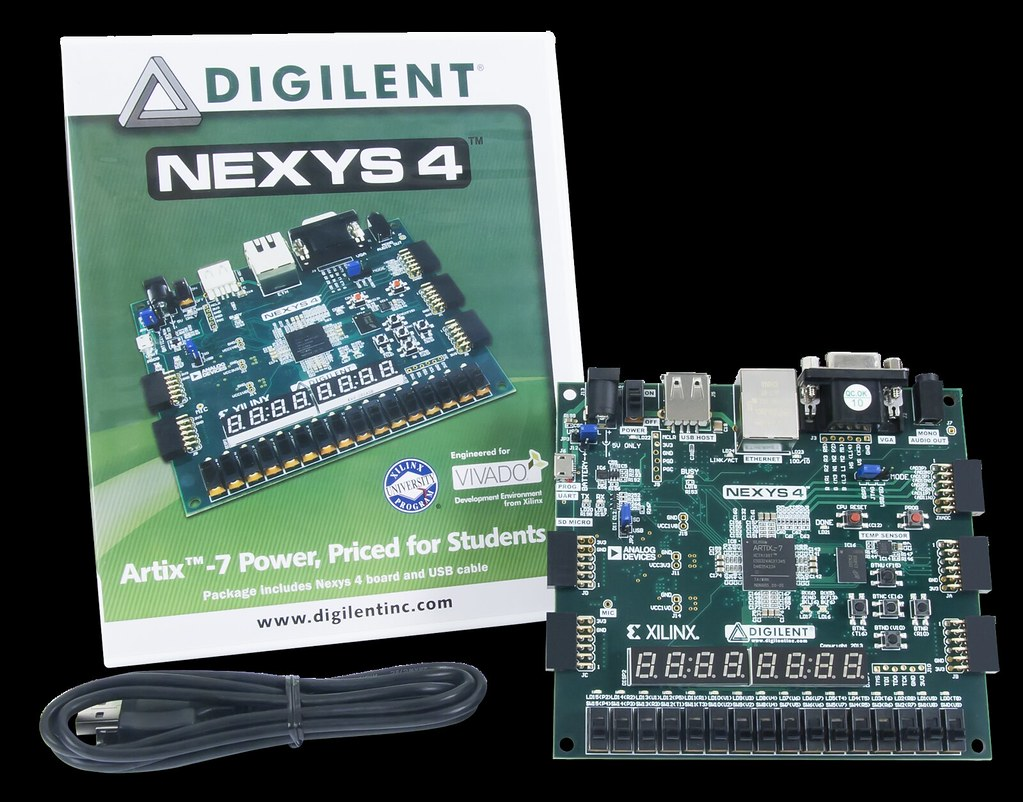
\includegraphics[width=0.4\linewidth]{images/img001_nexys4_board.jpg}
  \end{center}

  Documentatie:

  \begin{itemize}
    \item \url{https://reference.digilentinc.com/reference/programmable-logic/nexys-4/reference-manual}
    \item \url{https://reference.digilentinc.com/\_media/reference/programmable-logic/nexys-4/nexys4\_rm.pdf}
  \end{itemize}
\end{minipage}

\begin{minipage}{\linewidth}
  \subsection{Het Nexys4DDR-bord}

  Niet meer geproduceerd, maar nog wel verkrijgbaar via sommige websites met oude voorraad.

  \begin{center}
    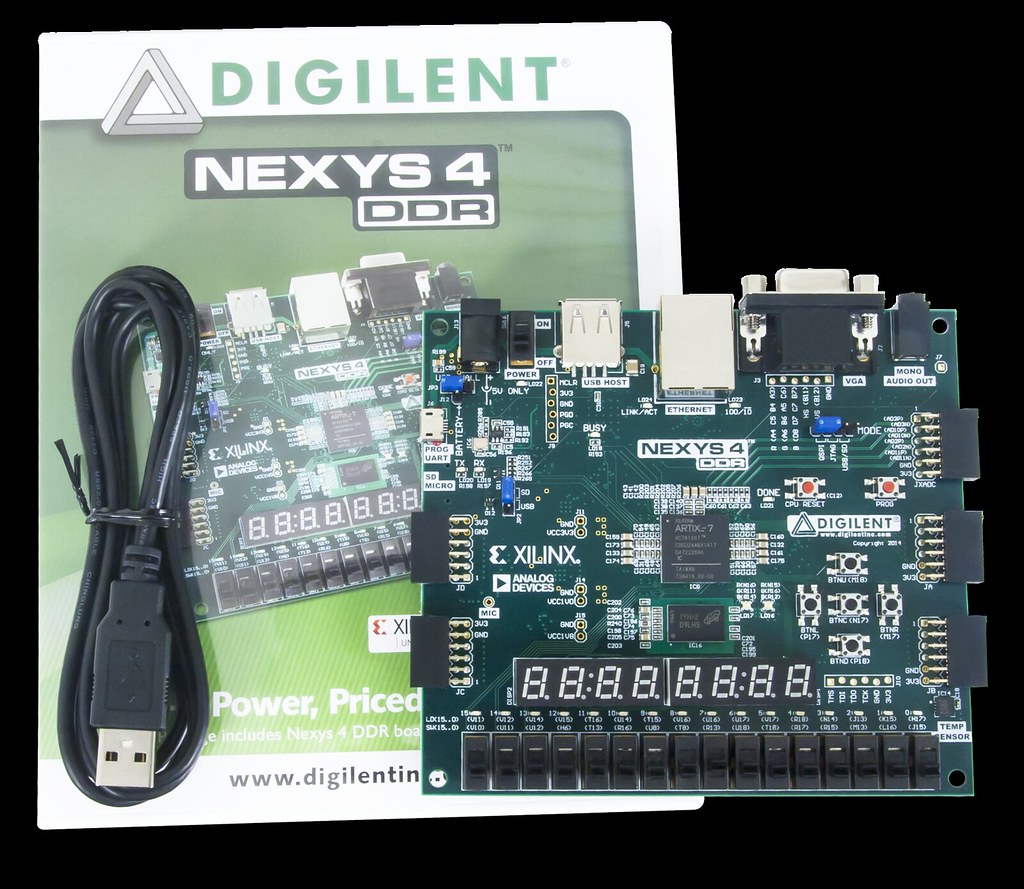
\includegraphics[width=0.4\linewidth]{images/img002_nexys4_ddr_board.jpg}
  \end{center}

  Documentatie:

  \begin{itemize}
    \item \url{https://reference.digilentinc.com/reference/programmable-logic/nexys-4-ddr/reference-manual}
    \item \url{https://reference.digilentinc.com/\_media/reference/programmable-logic/nexys-4-ddr/nexys4ddr\_rm.pdf}
  \end{itemize}
\end{minipage}

\begin{minipage}{\linewidth}
  \subsection{De Nexys A7}

  Dit is het bovenstaande Nexys4 DDR-bord, opnieuw uitgebracht onder een andere naam:

  \begin{center}
    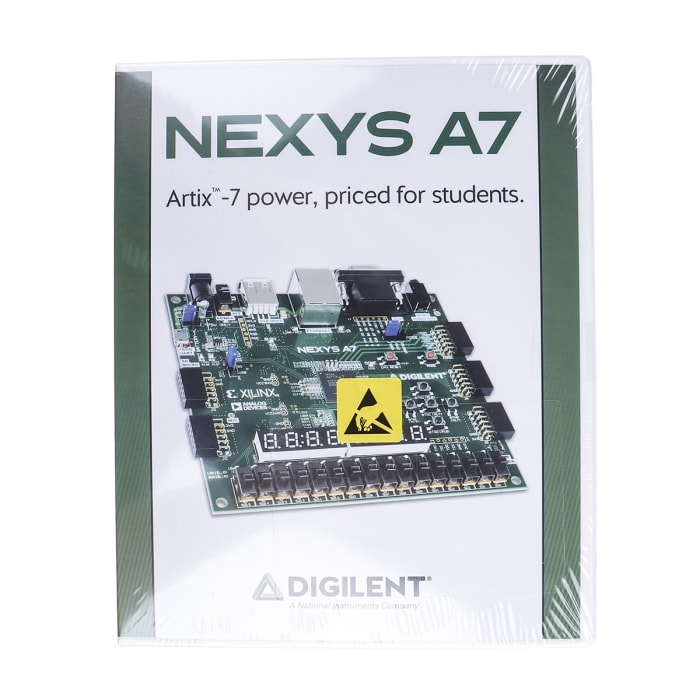
\includegraphics[width=0.4\linewidth]{images/img003_nexysA7_board.jpg}
  \end{center}

  Documentatie:

  \begin{itemize}
    \item \url{https://reference.digilentinc.com/reference/programmable-logic/nexys-a7/reference-manual}
    \item \url{https://reference.digilentinc.com/\_media/reference/programmable-logic/nexys-a7/nexys-a7\_rm.pdf}
  \end{itemize}
\end{minipage}

\newpage

\section{Stroom, jumpers, schakelaars en knoppen}

Deze foto van bovenaf toont de belangrijkste jumperposities op het Nexys4-bord:

  \begin{center}
    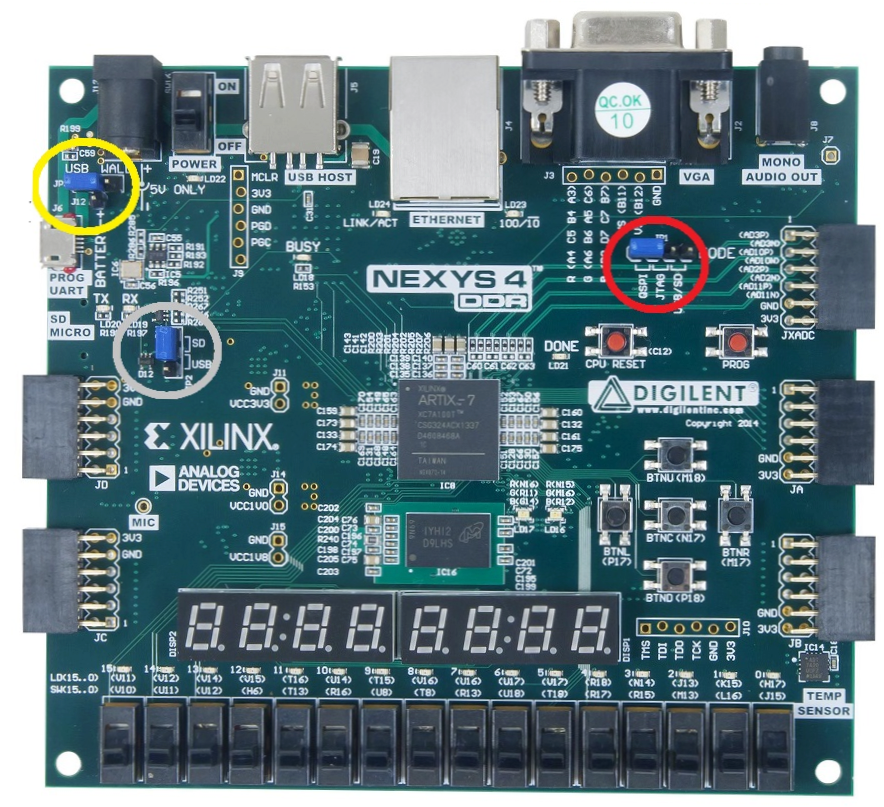
\includegraphics[width=0.9\linewidth]{images/nexys4_jumpers.png}
  \end{center}

De Nexys4-borden kunnen op twee manieren van stroom worden voorzien: via een externe voeding of via een standaard USB-poort.

\subsection{Micro-USB-voeding}

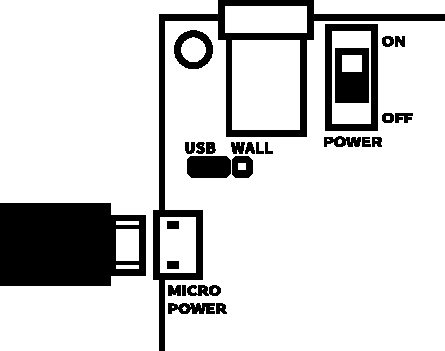
\includegraphics[width=5cm]{images/illustrations/nexys-micro-usb-power.pdf}

Sluit uw micro-USB-kabel aan op een USB-poort van een USB-lader of pc om stroom te leveren. Sluit het andere uiteinde aan op de micro-USB-connector van de Nexys4. Plaats de JP3-jumper op pennen 1 en 2 om USB-voeding te selecteren. Gebruik de schakelaar om de Nexys4 in te schakelen.

\subsection{Externe voeding}

\hspace*{1.7cm}
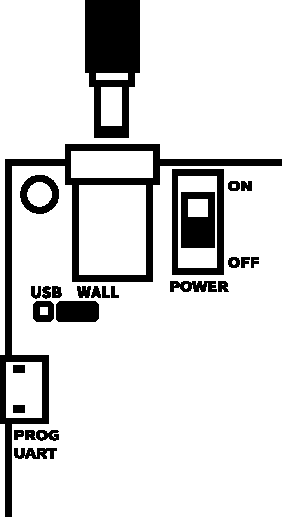
\includegraphics[width=3.2cm]{images/illustrations/nexys-power-supply.pdf}

De MEGA65-core kan veel stroom verbruiken en een standaard USB-poort kan in potentie te weinig vermogen leveren voor het Nexys4-bord. Het schrijven naar de SD-kaart kan met name vastlopen of vreemd gedrag vertonen. U wordt dan aangeraden een voeding van 5V te gebruiken.

Digilent verkoopt een voeding voor het Nexys4-bord en wij raden u aan deze te gebruiken om het risico op schade aan uw Nexys4-bord te vermijden. De gekozen voeding moet een center-positieve stekker met een binnendiameter van 2.1 mm hebben en 4.5VDC tot 5.5VDC leveren met een stroomsterkte van ten minste 1 ampère.

Sluit de voedingskabel aan op de voedingsaansluiting van de Nexys4. Plaats de JP3-jumper op pennen 2 en 3 om netvoeding te selecteren. Gebruik de schakelaar om de Nexys4 in te schakelen.

\subsection{Overige jumpers en schakelaars}

Voor uw eerste installatie raden wij u aan de volgende jumpers op uw Nexys4-bord in te stellen:

\begin{itemize}
  \item{JP1} - USB/SD  \item{JP2} - SD
\end{itemize}

\begin{center}
  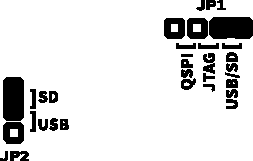
\includegraphics[width=3.2cm]{images/illustrations/nexys-jumpers.pdf}
\end{center}

Dit zorgt ervoor dat de bitstream-bestanden bij het opstarten vanaf uw SD-kaart geladen worden.

Op een later moment kunt u ervoor kiezen de bitstream vanaf de ingebouwde QSPI-flash te laden. In dat geval kunt u de instelling van de JP1-jumper aanpassen naar de QSPI-positie.

% XXX - Image of board highlighting the jumpers

Alle 16 schakelaars aan de onderkant van het bord moeten op de uit-positie staan.


\subsection{Aansluitingen en randapparatuur}

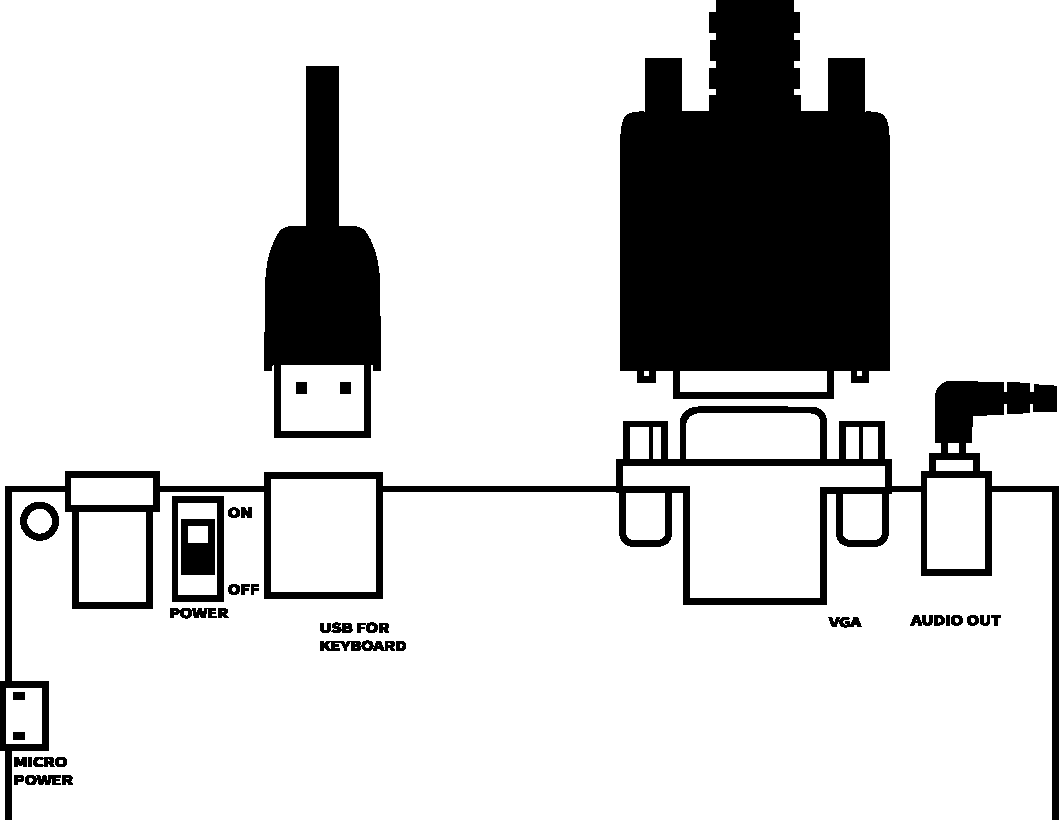
\includegraphics[width=\linewidth]{images/illustrations/nexys-connectors.pdf}

Aan de USB-poort kan een USB-toetsenbord worden aangesloten. Alleen een toetsenbord zonder USB-hub werkt met het Nexys4-bord. Over het algemeen werken zeer goedkope toetsenborden, terwijl duurdere toetsenborden vaak een USB-hub bevatten en niet werken. Het zou kunnen voorkomen dat u meerdere toetsenborden moet proberen voordat u er een vindt die werkt.

Aan de VGA-poort kan een VGA-beeldscherm worden aangesloten.

De mono-audio-uitgang kan worden aangesloten op de line-in van een versterker.


\subsection{Communicatie met uw pc}

Er kunnen situaties zijn waarin u vanaf uw pc met het Nexys4-bord wilt communiceren, bijvoorbeeld om de volgende activiteiten uit te voeren:

\begin{itemize}
  \item Het QSPI-flashgeheugen flashen via Vivado  \item Bitstream-bestanden rechtstreeks vanaf uw pc uploaden (via het m65-hulpprogramma)  \item Hulpprogramma's gebruiken zoals M65Connect, m65, mega65\_ftp, m65dbg, enz.
\end{itemize}

In zulke gevallen moet u de micro-USB-kabel op uw pc aansluiten.

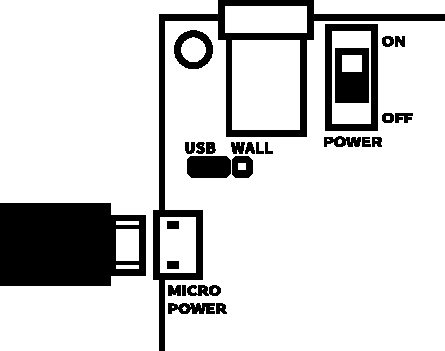
\includegraphics[width=5cm]{images/illustrations/nexys-micro-usb-power.pdf}

\subsection{Knoppen op het bord}

\begin{center}
  
\includegraphics[width=3.2cm]{images/illustrations/nexys-reset-buttons.pdf}
\end{center}

De ``CPU RESET''-toets reset de MEGA65 wanneer u deze indrukt, terwijl de ``PROG''-toets de FPGA zelf de MEGA65-core laat herladen. Het belangrijkste verschil tussen de twee is dat CPU RESET sneller is en de inhoud van het geheugen niet wist, terwijl de FPGA-knop langzamer is en de inhoud van het geheugen wel reset.

\begin{center}
  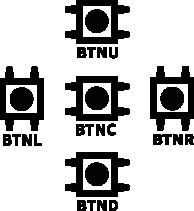
\includegraphics[width=3.2cm]{images/illustrations/nexys-five-buttons.pdf}
\end{center}

Twee van de vijf toetsen in de kruisopstelling kunnen eveneens worden gebruikt: BTND gedraagt zich alsof u \widekey{RESTORE} heeft ingedrukt, terwijl BTNC een interrupt activeert, alsof de IRQ-lijn naar massa is getrokken.

\section{Toetsenbord}

De toetsenbordindeling is positioneel en niet logisch. Dit betekent dat toetsen die zich in dezelfde positie bevinden als de toetsen op een C65-toetsenbord een vergelijkbare functie hebben. Deze relatie gaat ervan uit dat uw USB-toetsenbord een Amerikaanse toetsenbordindeling gebruikt.

Om u te helpen bij het vinden van de toetstoewijzingen van de diverse MEGA65-toetsen, beschikt de MEGA65 over een ingebouwde virtuele toetsenbordtest. Deze is op twee manieren te bereiken.

De eenvoudigste manier is om \specialkey{ALT} ingedrukt te houden terwijl u de Nexys4 inschakelt, of de Nexys4 reset met de ``PROG''-toets. Het configuratiemenu wordt weergegeven en door op 3 te drukken, verschijnt het virtuele toetsenbord op een zwarte achtergrond.

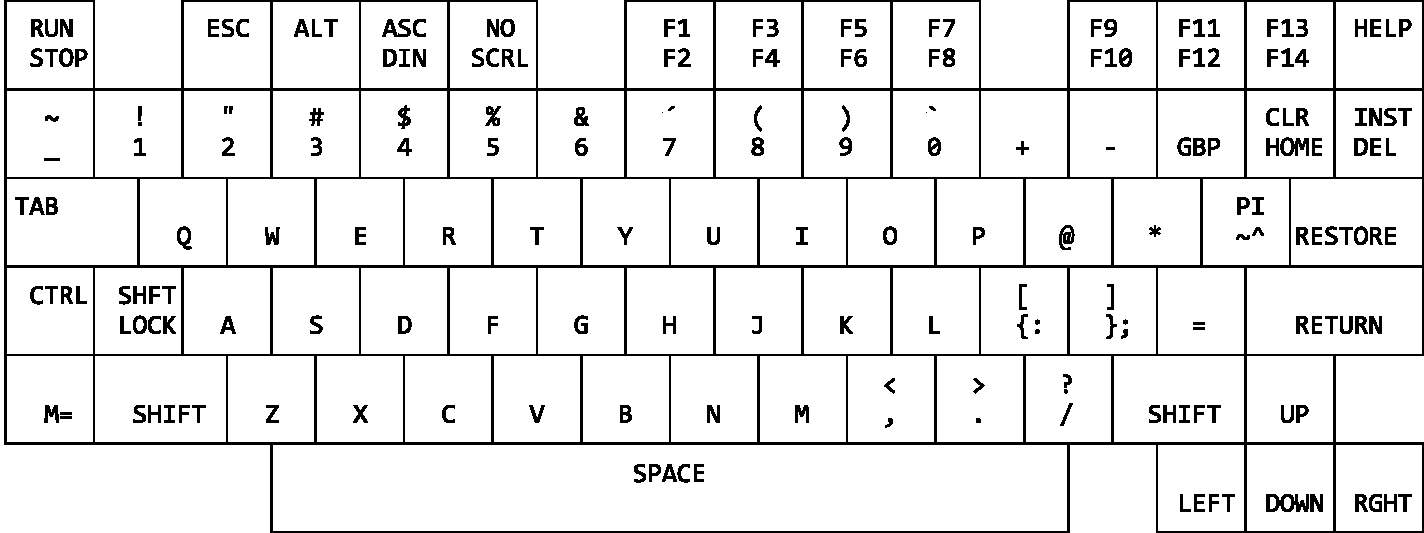
\includegraphics[width=\linewidth]{images/illustrations/virtual-keyboard.pdf}

Wanneer u een toets op het USB-toetsenbord indrukt, wordt de betreffende toets op het virtuele toetsenbord gemarkeerd weergegeven om u te helpen bij het herkennen van de toetstoewijzing.

De andere manier om het virtuele toetsenbord te bereiken is vanuit de MEGA65 zelf. Houd \megasymbolkey ingedrukt en druk op \specialkey{TAB} om de Matrix Mode Debugger te openen. Voer vervolgens het volgende in:

\screentextwide{s ffd3615 ff}

Dit opent een halfdoorzichtig virtueel toetsenbord aan de bovenkant van het scherm. Als alternatief:

\screentextwide{s ffd3615 ff ff}

Dit opent een halfdoorzichtig virtueel toetsenbord in het midden van het scherm.

Houd \megasymbolkey ingedrukt en druk op \specialkey{TAB} om de Matrix Mode Debugger te verlaten en terug te keren naar de MEGA65.

\subsection{Enkele toetstoewijzingen met een USB-toetsenbord}

\widekey{RESTORE} is toegewezen aan de Page Up-toets.

\specialkey{RUN\\STOP} is toegewezen aan \specialkey{ESC}.

\newpage

\section{MicroSDHC-kaart voorbereiden}

De MEGA65 vereist een SDHC-kaart met een capaciteit van 4 GB tot 64 GB. Sommige SDXC-kaarten kunnen werken, maar dit wordt niet officieel ondersteund.

De voorbereidingsstappen voor de SD-kaart van het Nexys4-bord komen grotendeels overeen met de stappen die nodig zijn voor echte MEGA65-hardware. Het is dan ook de moeite waard om een kijkje te nemen in
\ifdefined\printmanual
het {\bf grote Mega65-boek}
\else
\bookvref{cha:configuringyourmega}
\fi
als u ooit meer details nodig heeft.

In dit onderdeel bespreken we de specifieke stappen uitgebreider en beperken we ons tot een beknopte behandeling van de gemeenschappelijke stappen.

Een verschil tussen het Nexys-bord en de echte MEGA65-hardware is dat laatstgenoemde standaard een bitstream/core bevat waarmee u uw SD-kaart in de specifieke indeling kunt formateren die door de MEGA65 wordt vereist.

Voor eigenaren van het Nexys4-bord is er echter geen standaard bitstream; raadpleeg daarom het {\bf grote Mega65-boek} voor meer informatie over waar u de juiste bestanden ``nexys4.bit of ``nexys4ddr-widget.bit voor uw apparaat kunt downloaden.

\subsection{Voorbereidingsstappen}

De stappen zijn:

\begin{itemize}
  \item{Formateer de SD-kaart} op een handige computer met het FAT32-bestandssysteem. De MEGA65- en Nexys4-borden ondersteunen geen andere bestandssystemen, met name niet het exFAT-bestandssysteem.\item{Kopieer} uw bitstream-bestand (met een bestandsnaam die eindigt op ``.bit'') naar de SD-kaart.\item{Plaats} de SD-kaart in de SD-kaartsleuf aan de onderkant van het Nexys4-bord.\item{Schakel} het Nexys4-bord in.\item{Open het hulpprogrammamenu} door \specialkey{ALT} ingedrukt te houden op het USB-toetsenbord dat op het Nexys4-bord is aangesloten wanneer het MEGA65-startscherm wordt weergegeven.\item{Open het FDISK/FORMAT-hulpprogramma} door op 2 te drukken wanneer de optie verschijnt op het MEGA65-opstartscherm.\item{Volg de aanwijzingen} in het FDISK/FORMAT-programma om de SD-kaart opnieuw te formatteren voor gebruik door de MEGA65. \\
  \\
  Het FDISK-hulpprogramma maakt twee partities op uw SD-kaart aan en formatteert deze.
  \begin{itemize}
    \item De ene is type \$41 = MEGA65-systeempartitie, waar de opslagslots, configuratiegegevens en andere bestanden staan. \\  (Deze partitie is onzichtbaar op bijvoorbeeld Windows-pc's).    \item De andere partitie met type \$0C = VFAT32, waar KERNAL, ondersteuningsbestanden, spellen enzovoort later naartoe worden gekopieerd. \\  (Deze partitie is zichtbaar op bijvoorbeeld Windows-pc's).
  \end{itemize}
\item{Zodra het formatteren is voltooid}, schakelt u het Nexys4-bord uit en verwijdert u de microSDHC-kaart uit het Nexys-bord en plaatst u deze terug in uw pc\item{Kopieer} deze keer de volgende items naar de SD-kaart:
  \begin{itemize}
    \item Het bitstream-bestand    \item De uitgepakte bestanden uit het ``\textbf{SD essentials.rar}''-of het ``\textbf{SD essentialsNoROM.rar}''-bestand dat u van de MEGA65-filehost hebt gedownload.    \item{Als u uw eigen voorkeurs-ROM-bestand hebt} (bijvoorbeeld ``\textbf{911001.BIN}''), kopieer dit ook naar de SD-kaart en hernoem het naar ``\textbf{MEGA65.ROM}'' (hoofdletters zijn verplicht).    \item{Eventuele .D81-schijfimage-bestanden} waarvan u gebruik wilt maken.
      \begin{itemize}
        \item Let op: wanneer een bestand met de naam MEGA65.D81 aan de SD-kaart wordt toegevoegd, wordt dit automatisch gemonteerd bij het opstarten.        \item Zorg ervoor dat alle .D81-bestanden namen hebben die voldoen aan de oude DOS 8.3-tekenlimiet en in hoofdletters zijn geschreven. Deze beperking wordt in een toekomstige versie verwijderd.
      \end{itemize}
  \end{itemize}
\item{Verwijder de SD-kaart} en plaats deze terug in uw Nexys4-bord.\item{Schakel het Nexys4-bord} weer in. De MEGA65 zou binnen 15 seconden moeten opstarten.\item"Bij de eerste opstart bevindt u zich op het onboarding-scherm, waarvan meer details te vinden zijn in
\ifdefined\printmanual
het {\bf grote Mega65-boek}
\else
\bookvref{cha:configuringyourmega}
\fi
.

\end{itemize}

Gefeliciteerd. Uw MEGA65 is ingesteld en gereed voor gebruik.

Houd er rekening mee dat bij de bovenstaande methode het bitstream-bestand naar de SD-kaart wordt gekopieerd, waardoor de Nexys-FPGA de bitstream bij elke opstartcyclus laadt; het opstarten duurt dan ongeveer 13 seconden. De bitstream kunt u ook met Vivado-software naar het QSPI-flashgeheugen flitsen; de opstarttijd verkort u daarmee tot 0.3 seconden.

Voor meer gedetailleerde informatie over het voorbereiden en configureren van uw MEGA65 verwijzen wij u naar
\ifdefined\printmanual
het {\bf grote Mega65-boek}
\else
\bookvref{cha:configuringyourmega}
\fi
hoofdstuk.

\section{De bitstream laden vanuit QSPI}

Hoewel het laden van de bitstream vanaf de SD-kaart de aanbevolen (en veelbewandelde) route is die dit document heeft gekozen, hebben de laatste tijd meer Nexys4-gebruikers de alternatieve weg verkend om de bitstream vanuit het QSPI-flashgeheugen te laden. Enkele mogelijke redenen hiervoor zijn:

\begin{itemize}
  \item Snellere opstarttijden (0,3 seconden versus 13 seconden)  \item Sommige gebruikers waren geïnteresseerd in de mogelijkheid om meerdere cores op hun QSPI te flitsen (via stappen die beschreven staan in de
\ifdefined\printmanual
het {\bf grote Mega65-boek}
\else
\bookvref{cha:cores}
\fi
		Hoofdstuk)  \item Sommige gebruikers hebben last gehad van hardnekkige problemen met de route via de SD-kaart, zoals:
    \begin{itemize}
      \item Het systeem kan niet opnieuw opstarten vanaf het onboarding-scherm      \item Het systeem kan niet opnieuw opstarten vanuit het freeze-menu na het wisselen tussen PAL/NTSC
    \end{itemize}
\end{itemize}

Indien dit in de toekomst een populairdere route blijkt te zijn, kunnen wij onze documentatie hierop aanpassen. Hier volgen enkele stappen in het kort.

\subsection{Voorbereidingsstappen}

Als u deze route wilt proberen, moet u de JP1-jumperinstelling aanpassen om QSPI te gebruiken en vervolgens de stappen volgen in het hoofdstuk \nameref{cha:fpgacpldflashing} met betrekking tot \nameref{sec:installvivado} en \nameref{sec:mainfpgaflashing}.

Houd er rekening mee dat de installatie van Vivado een langdurig proces is (zowel wat betreft de downloadtijd als de installatietijd).

Nadat u Slot0 van uw QSPI-chip hebt geflitst via Vivado, kunt u de stappen volgen die beschreven staan in
\ifdefined\printmanual
het {\bf grote Mega65-boek}
\else
\bookvref{cha:configuringyourmega}
\fi
voor de aangepaste SD-kaartformattering, het installeren van ROM- en ondersteuningsbestanden en de onboarding.

\section{Widget-bord}

Als u een Nexys-bord bezit (alle modellen), vindt u het wellicht interessant om een widget-bord aan uw Nexys-apparaat toe te voegen, zodat u verbinding kunt maken met:

\begin{itemize}
  \item{een originele C64- of C65-toetsenbord}
  \item{2 DB-9-joysticks}
  \item{Paddles of een 1351-muis}
  \item{Cartridges (werken nog niet)}
\end{itemize}

Het widget-bord wordt via de PMOD-connectoren met uw Nexys-bord verbonden.

Momenteel is het alleen verkrijgbaar als onbewerkte printplaat (zonder componenten), hier aan te schaffen:

\begin{itemize}
  \item \url{https://oshpark.com/shared\_projects/Y37xg9N7}
\end{itemize}

De firmware, de printplaatdiagrammen, het schema en de stuklijst zijn in het volgende GitHub-project te vinden:

\begin{itemize}
  \item \url{https://github.com/sy2002/DM65PIC}
\end{itemize}

U moet de onderdelen uit de stuklijst apart aanschaffen en de componenten zelf op het bord monteren.

Dit forum64.de-thread kan voor u van belang zijn wanneer u de ervaringen van anderen die dit proces hebben doorlopen wilt lezen of wanneer u zelf vragen heeft:

\begin{itemize}
  \item \url{https://www.forum64.de/index.php?thread/90465-mega-65-ports-add-on-card-still-available-if-where}
\end{itemize}

De printplaatbestanden (c65Keyb.brd) en schematische bestanden (c65Keyb.sch) bevinden zich in de map ``eagle/' van het DM65PIC-project en kunnen worden bekeken met het gratis programma AutoDesk Eagle, hier beschikbaar:

\begin{itemize}
  \item \url{https://www.autodesk.com/products/eagle/free-download}
\end{itemize}

Hier volgen enkele foto's van het widget-bord in gebruik:
  \begin{center}
    \includegraphics[width=0.9\linewidth]{images/widget-board-martin.png}
  \end{center}
  \begin{center}
    \includegraphics[width=0.9\linewidth]{images/widget-board-deft1.png}
  \end{center}
  \begin{center}
    \includegraphics[width=0.9\linewidth]{images/widget-board-deft2.png}
  \end{center}

Voor het gemak zijn de printplaat- en schema's van het widget-bord eveneens opgenomen in \bookvref{sec:nexyswidgetschematics}.

Enkele aanvullende achtergrondnotities over het bord:

\begin{itemize}
  \item{Het widget-bord is oorspronkelijk bedoeld om in een C65-behuizing te passen}
  \item{De uitbreidingspoort is niet bruikbaar en er moet een stuk worden weggezaagd voor de C64-behuizing}
  \item{Het zou redelijk zijn het bord aan te passen voor gebruik in een C64-behuizing (wat zeker het meest voorkomende gebruik zal zijn)}
\end{itemize}

\section{PMOD-naar-joystick-adapter}

Als alternatief (en goedkoper) voor wie alleen een DB9-joystick-poort via de PMOD-connectoren wil toevoegen, heeft een community-lid, TheChief, een manier bedacht om dat te doen. Meer informatie is te vinden in het volgende Discord-thread:

\begin{itemize}
  \item \url{https://discord.com/channels/719326990221574164/903079038015389716/929369283119685643}
\end{itemize}

  \begin{center}
    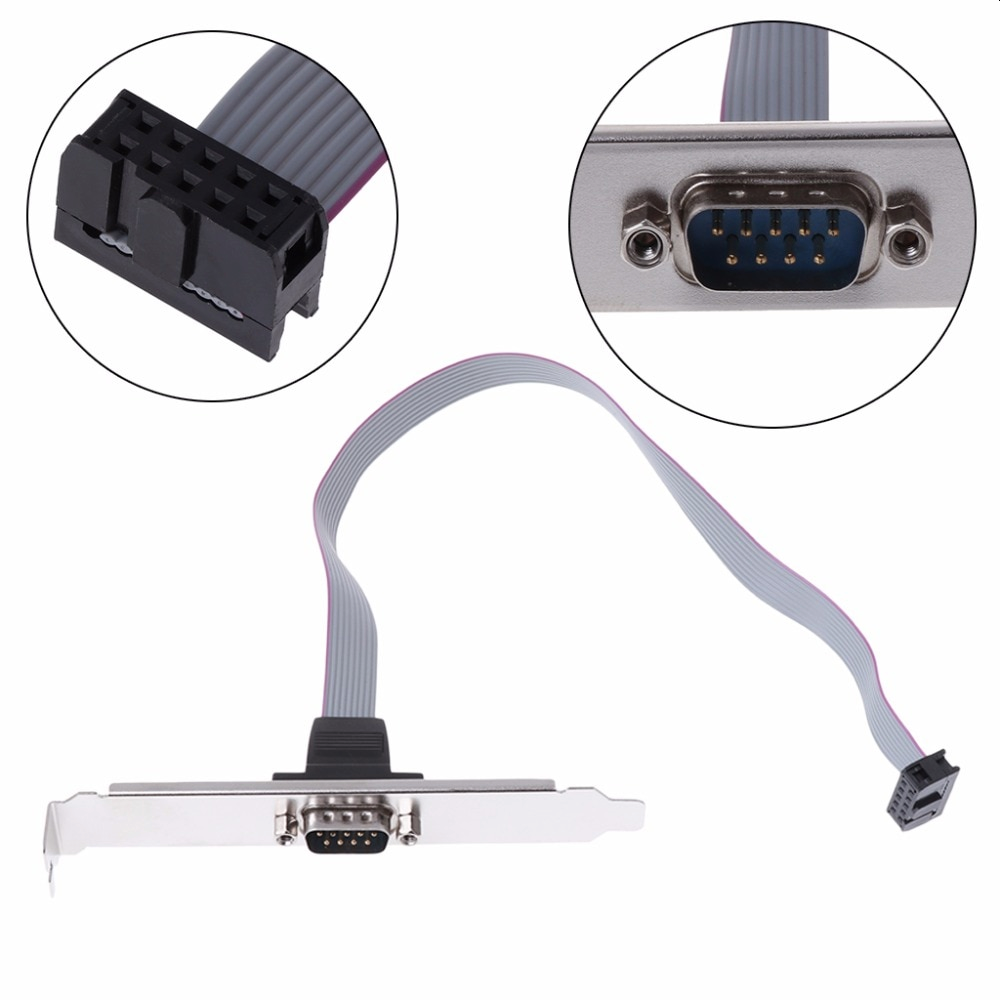
\includegraphics[width=0.9\linewidth]{images/joystick-pmod-thechief.png}
  \end{center}

\begin{minipage}{\linewidth}
\begin{center}
  \begin{longtable}{|L{3cm}|L{3cm}|p{3cm}|}
    \hline
    {\textbf{Joystick-actie}} & {\textbf{PMOD-JA-aansluitingen}} & {\textbf{DB9-aansluitingen}} \\
    \hline
    {Vuur} & {jahi(9)} & {pin 6} \\
    \hline
    {Omhoog} & {jalo(1)} & {pin 1} \\
    \hline
    {Links} & {jalo(2)} & {pin 3} \\
    \hline
    {Omlaag} & {jahi(7)} & {pin 2} \\
    \hline
    {Rechts} & {jahi(8)} & {pin 4} \\
    \hline
  \end{longtable}
\end{center}
\end{minipage}


\section{Handige tips}

Hier volgen enkele handige tips om vertrouwd te raken met de MEGA65:

\begin{itemize}

\item{Druk op \& houd \megasymbolkey (of de Commodore-toets als u een Commodore 64- of 65-toetsenbord gebruikt) ingedrukt tijdens het opstarten om in C64-modus op te starten in plaats van C65-modus.}
 \item{Druk op \& houd \specialkey{RUN\\STOP} ingedrukt tijdens het opstarten om de machine-taalmonitor te openen in plaats van BASIC te starten.}
\item{Druk op \widekey{RESTORE} en houd deze ongeveer een halve tot een seconde ingedrukt om het MEGA65 Freeze-menu te openen. Dit menu biedt handige hulpmiddelen om de processorsnelheid te wijzigen, te wisselen tussen PAL \& NTSC-videomodus, audio-instellingen aan te passen, freeze-states te beheren en D81-schijfimages te selecteren. U kunt bovendien het geheugen van het bevroren programma inspecteren en bewerken, en nog veel meer. Dit menu is in vele opzichten het hart van de MEGA65 en is het ontdekken zeker waard.}
\item{Typ \screentext{POKE0,65} in C64-modus om de processor op volle snelheid (40 MHz) te zetten. Sommige software gedraagt zich in deze modus onjuist, terwijl andere software juist sneller werkt.}
\item{Typ \screentext{POKE0,64} in C64-modus om de processor op 1 MHz te zetten.}
\item{Typ \screentext{SYS58552} in C64-modus om naar C65-modus te schakelen.}
\item{Typ \screentext{GO64} in C65-modus en bevestig door \screentext{Y} in te drukken om naar C64-modus te schakelen, hetzelfde als op een C128.}
\item{De C65-ROM maakt apparaat 8 tot standaard, zodat u het \textbf{,8} aan het einde van LOAD- en SAVE-commando's normaal gesproken kunt weglaten.}
\item{Het indrukken van \specialkey{SHIFT} + \specialkey{RUN\\STOP} in de C64- of C65-modus probeert van schijf op te starten.}
\end{itemize}

Veel plezier! Veel plezier! Er is jarenlang met liefde aan de MEGA65 gewerkt voor uw plezier. Wij hopen dat u er net zoveel plezier aan beleeft als wij bij het maken hebben gehad!

Het MEGA Museum of Electronic Games \& Art verwelkomt uw feedback, suggesties en bijdragen aan dit open-source-project voor het bewaren van digitaal erfgoed.


\part{BIJLAGEN}

\appendix
  \chapter{Het flashen van de FPGA's en CPLD's in de MEGA65}
\label{cha:fpgacpldflashing}

De MEGA65 is een computer met open-source hardware en open-source ontwerp. Dit betekent dat u niet alleen programma's kunt schrijven die op de MEGA65 als een voltooide computer draaien, maar ook de programmeerbare chips in de MEGA65 kunt gebruiken om er allerlei andere dingen van te maken.

Als u alleen een upgradecore voor de MEGA65 wilt installeren, of een core waarmee u uw MEGA65 als een ander type computer kunt gebruiken, kijkt u beter in \bookvref{cha:cores}.

Dit hoofdstuk is vooral bedoeld voor mensen die willen helpen bij het ontwikkelen van cores voor de MEGA65. Het kan ook interessant zijn voor eigenaren van Nexys4-borden die hun apparaten vanaf het QSPI-flashgeheugen op het bord willen opstarten (in plaats van een bitstreambestand vanaf de SD-kaart). Hiervoor moet een .mcs-bestand op de QSPI-chip van het bord geflashed worden om een initiële bitstream in de positie ``Slot 0'' te plaatsen.

Deze programmeerbare chips heten Field Programmable Gate Arrays (FPGA's) of Complex Programmable Logic Devices (CPLD's) en kunnen een breed scala aan circuits implementeren. Ze worden doorgaans geprogrammeerd met een taal zoals VHDL of Verilog. Dit zijn talen die de meeste mensen niet vaak tegenkomen. Ze zijn ook op een aantal punten heel anders dan ``normale'' programmeertalen en het kan even duren voordat u begrijpt hoe ze werken. Met enige inzet en volharding kunt u echter spannende dingen ermee creëren.

\section{Aanbevolen specificaties voor de pc}

Reken erop dat u vele gigabytes aan software moet installeren op een Linux- of Windows-pc voordat u programma's kunt schrijven voor de FPGA's en CPLD's in de MEGA65. Het ``compileren'' van complexe ontwerpen kan ook enkele uren duren, afhankelijk van de snelheid en het geheugen van uw computer. Wij raden een computer met ten minste 12 GB RAM (bij voorkeur 16 GB) aan als u programma's voor FPGA's en CPLD's wilt schrijven. Als u daarentegen alleen programma's op de FPGA's en CPLD's van uw MEGA65 wilt laden die door anderen zijn geschreven, volstaan de meeste computers met een recente versie van Windows of Linux.

\begin{itemize}
  \item \underline{Besturingssysteem}: Linux of Windows  \item \underline{Snelheid van de processor}: zo snel als u kunt vinden!  \item \underline{Aantal cores}: bij voorkeur 8 of meer, omdat de gratis licentie van Vivado maximaal 8 cores kan gebruiken.  \item \underline{Harde schijf}: ongeveer 70 GB of meer. De exacte hoeveelheid hangt af van hoeveel onderdelen van Vivado u installeert (hou er rekening mee dat het volledige installatiebestand zelf ongeveer 50 GB is)  \item \underline{Geheugen}: minimaal 12 GB (bij voorkeur meer, voor de zekerheid)
\end{itemize}

\section{Waarschuwing}

Voordat we verdergaan, moeten we u waarschuwen voor het opnieuw programmeren van de FPGA's en CPLD's in de MEGA65. Het opnieuw programmeren van de FPGA van de MEGA65 kan schade veroorzaken of uw MEGA65 in een onbereikbare staat achterlaten waarvan het moeilijk is te herstellen, oftewel ``gebrickt''. Als u ervoor kiest om uw MEGA65 te openen en een van de FPGA's erin opnieuw te programmeren, kunnen wij de correcte werking van het apparaat niet langer garanderen. Wij kunnen de fabrieksgarantie van het apparaat als computer derhalve niet meer redelijkerwijs honoreren. U bent gewaarschuwd!

\section{Vivado installeren}
\label{sec:installvivado}

U moet Vivado installeren om het QSPI-flashgeheugen in uw doelapparaat te flashen, of het nu een MEGA65 R2/R3/R3A/R4, Nexys4/Nexys4DDR/NexysA7, MEGAphone of ander apparaat is.

Vivado is ook het hulpprogramma dat wordt gebruikt voor het compileren (beter bekend als synthese) van FPGA-bitstreams.

Ga naar \url{https://www.xilinx.com/support/download.html}

\begin{minipage}{\linewidth}
  Selecteer versie 2020.2
  \\
  \begin{center}
    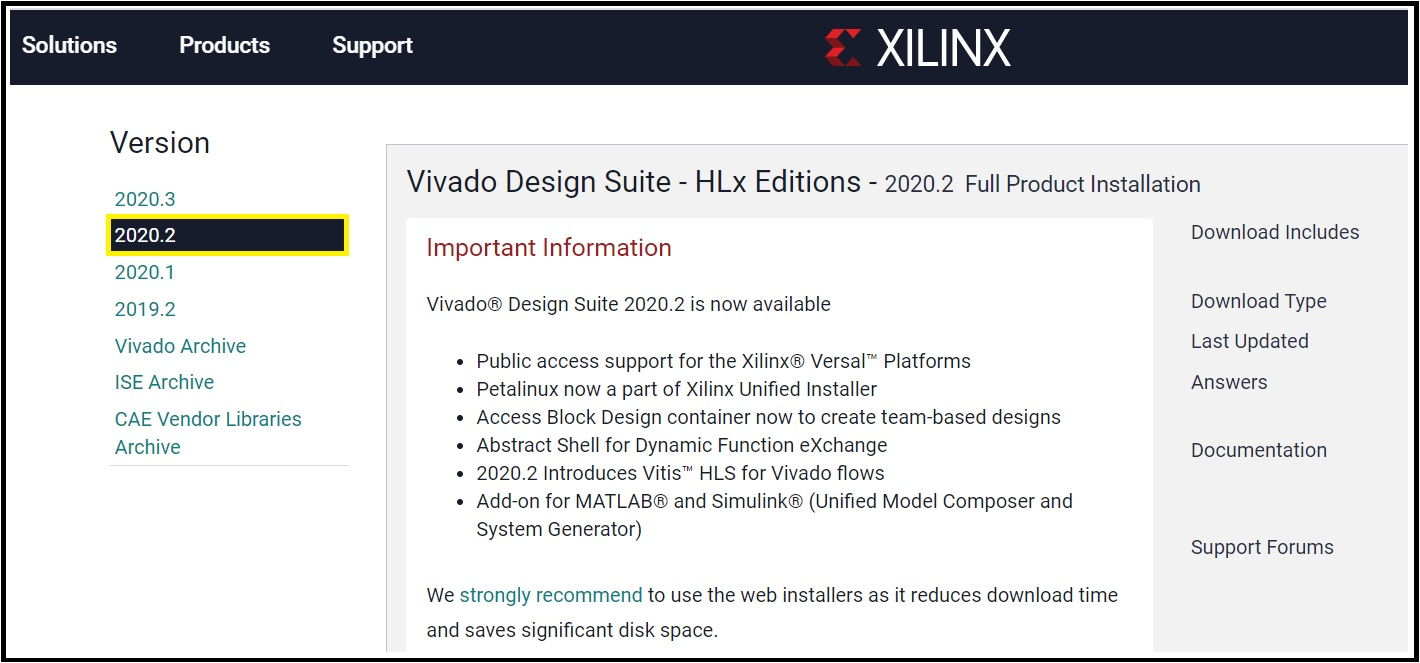
\includegraphics[width=\linewidth]{images/VivadoInstimg002.jpg}
  \end{center}
  Opmerking: sommige gebruikers hebben nog succes met oudere versies, omdat het hoofddoel hier is om een versie te installeren die de FPGA van uw doelhardware ondersteunt. \\
  \\
  Dat wil zeggen de Artix7 100T (voor Nexys en R2) of 200T (R3/R3A/R4).
\end{minipage}

\begin{minipage}{\linewidth}
  Klik op Xilinx Unified Installer 2020.2: Windows Self Extracting Web Installer EXE - 248.44MB
  \\
  \begin{center}
    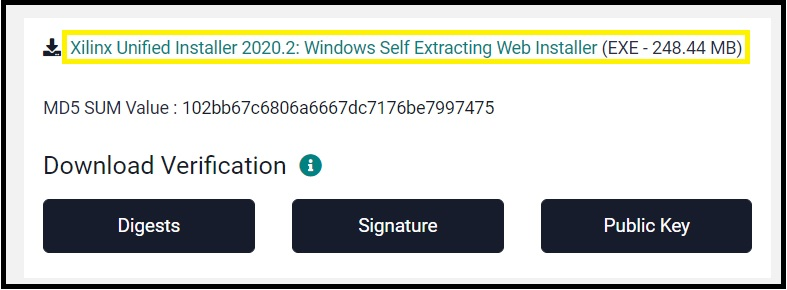
\includegraphics[width=0.8\linewidth]{images/VivadoInstimg003.jpg}
  \end{center}
\end{minipage}

\begin{minipage}{\linewidth}
  U wordt gevraagd een account aan te maken om in te kunnen loggen en het installatieprogramma te kunnen downloaden. \\
  \\
  Uw inloggegevens worden ook gevraagd tijdens de installatie.
  \\
  \begin{center}
    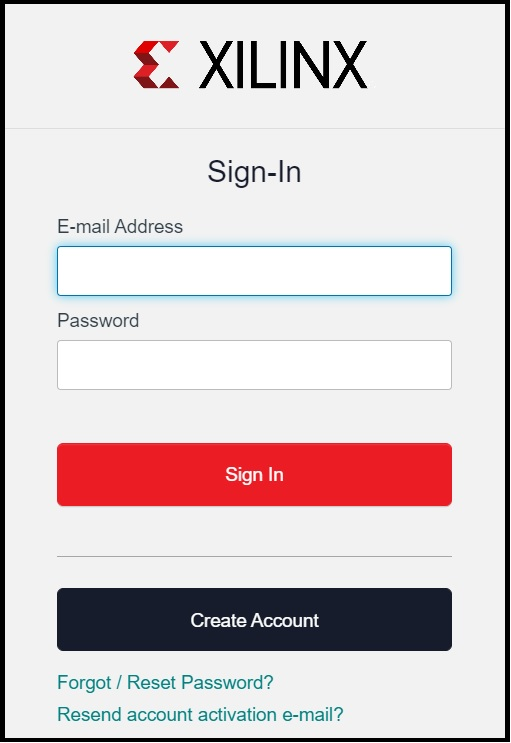
\includegraphics[width=0.3\linewidth]{images/VivadoInstimg004.jpg}
  \end{center}
\end{minipage}

\begin{minipage}{\linewidth}
  Nadat u ingelogd bent, moet u enkele persoonlijke gegevens invullen en dan op Download klikken.
  \\
  \begin{center}
    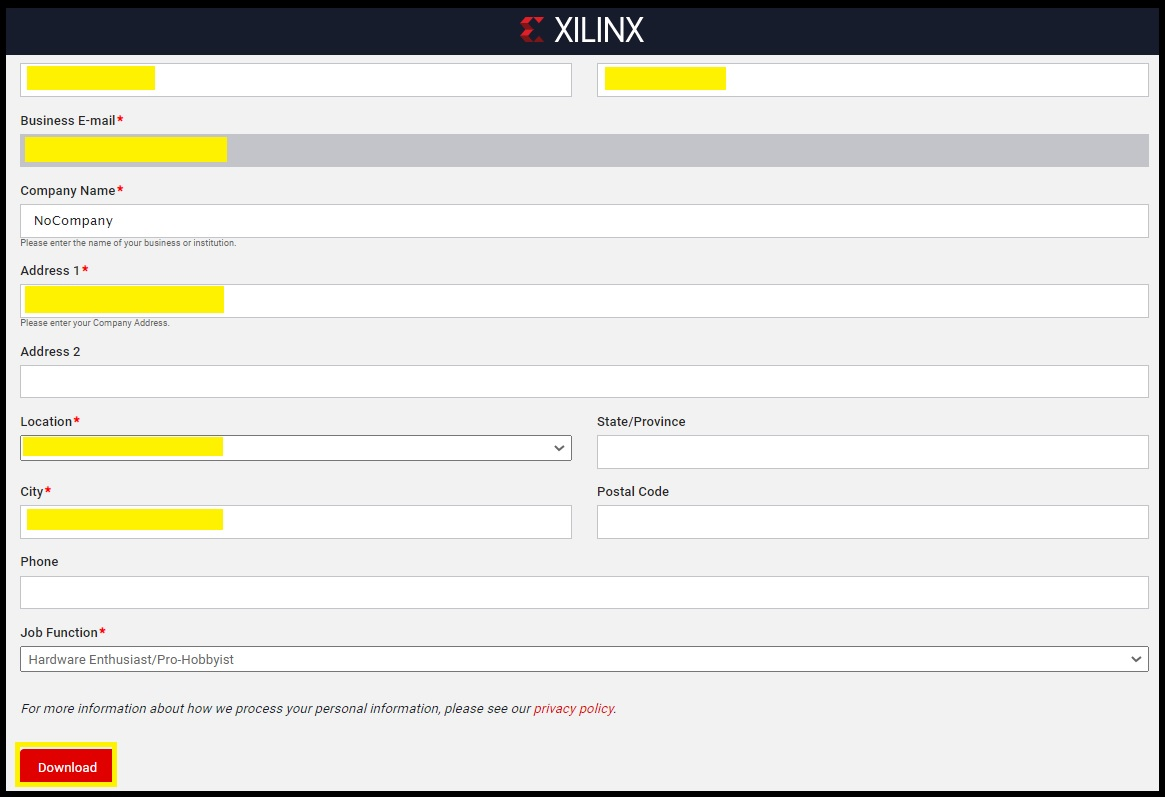
\includegraphics[width=0.8\linewidth]{images/VivadoInstimg005.jpg}
  \end{center}
\end{minipage}

\begin{minipage}{\linewidth}
  Voer het installatieprogramma uit als beheerder (Xilinx\_Unified\_2020.2\_1118\_1232\_Win64.exe).
  \\
  \begin{center}
    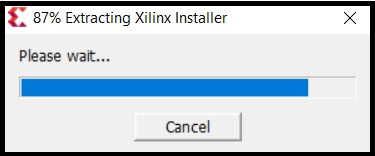
\includegraphics[width=0.5\linewidth]{images/VivadoInstimg006.jpg}
  \end{center}
\end{minipage}

\begin{minipage}{\linewidth}
  Klik op Allow Access.
  \\
  \begin{center}
    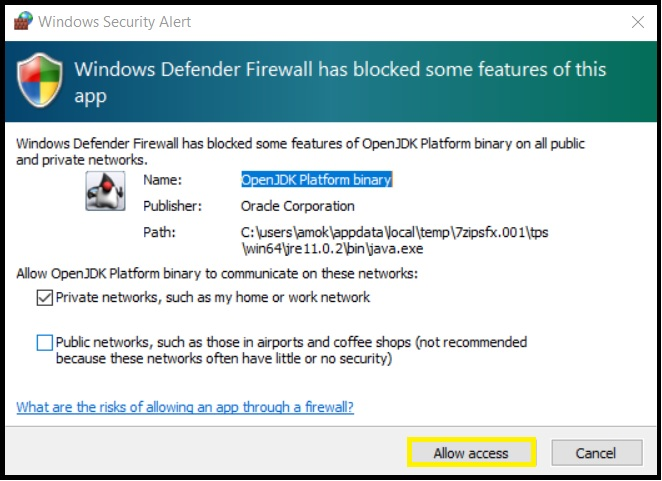
\includegraphics[width=0.5\linewidth]{images/VivadoInstimg007.jpg}
  \end{center}
\end{minipage}

\begin{minipage}{\linewidth}
  Klik op Next.
  \\
  \begin{center}
    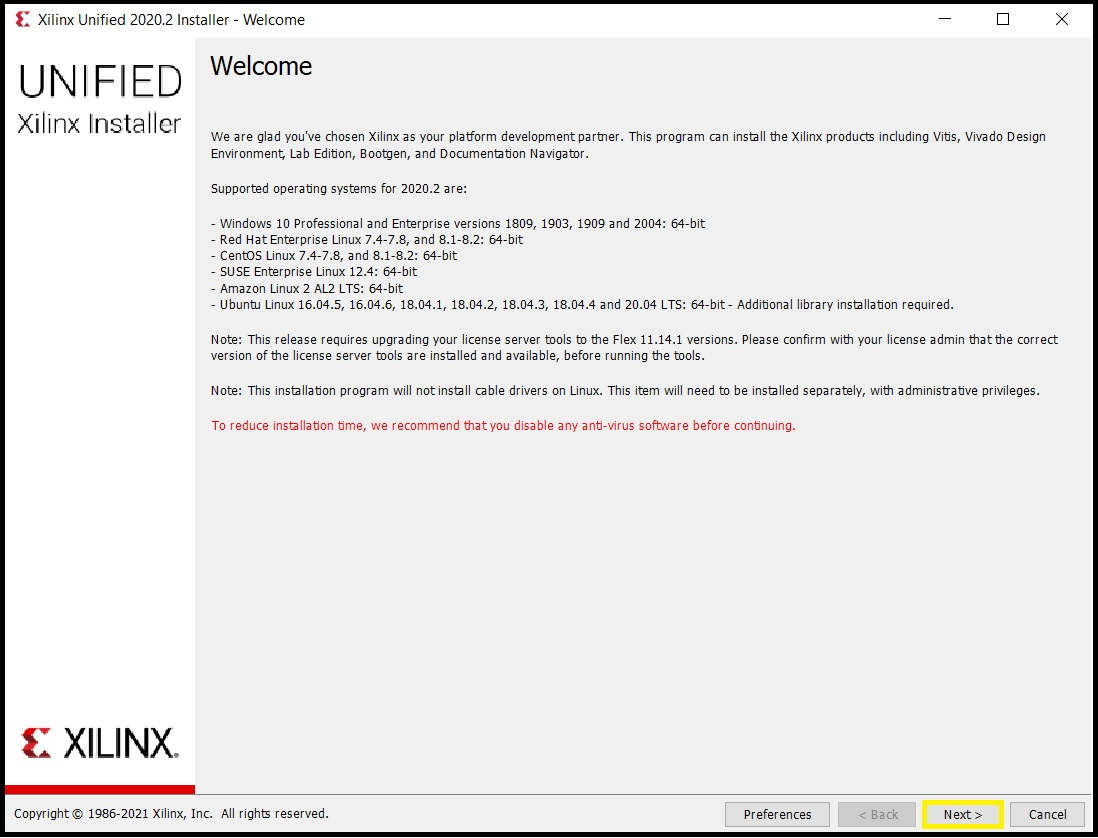
\includegraphics[width=0.7\linewidth]{images/VivadoInstimg008.jpg}
  \end{center}
\end{minipage}

\begin{minipage}{\linewidth}
  Voer uw inloggegevens in en klik op Next.
  \\
  \begin{center}
    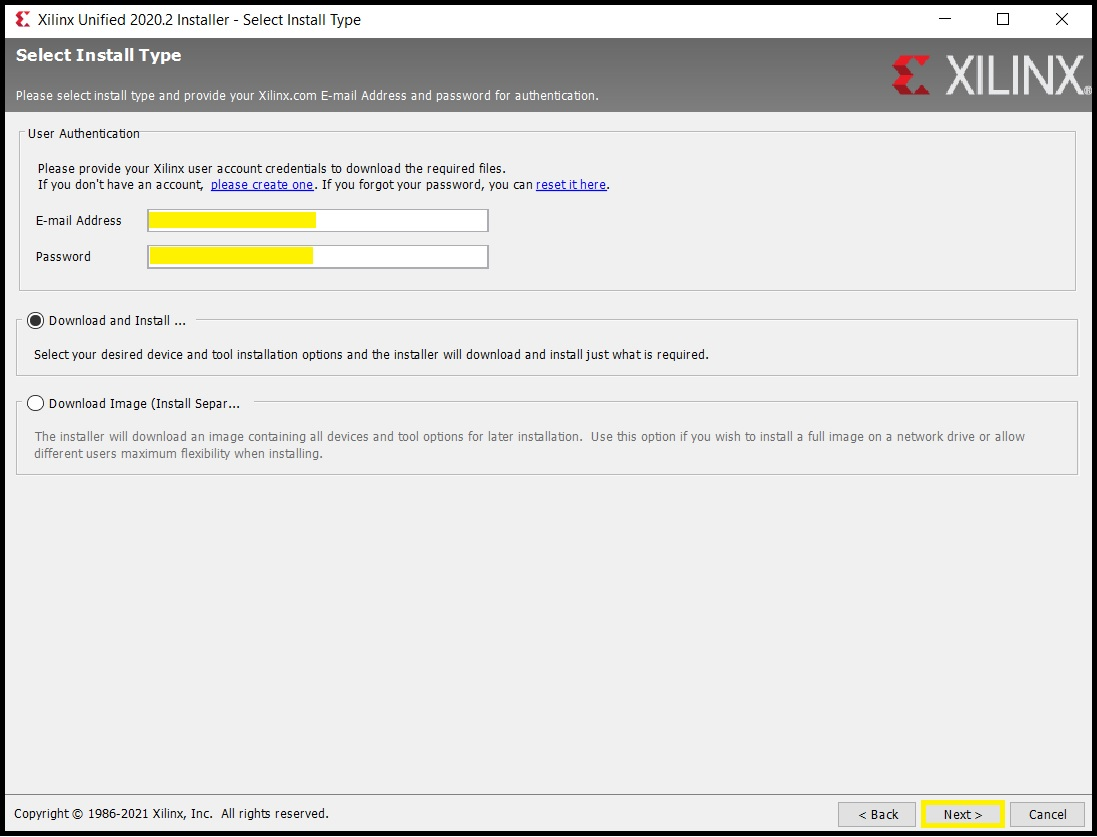
\includegraphics[width=0.7\linewidth]{images/VivadoInstimg009.jpg}
  \end{center}
\end{minipage}

\begin{minipage}{\linewidth}
  Selecteer Vivado en klik op Next.
  \\
  \begin{center}
    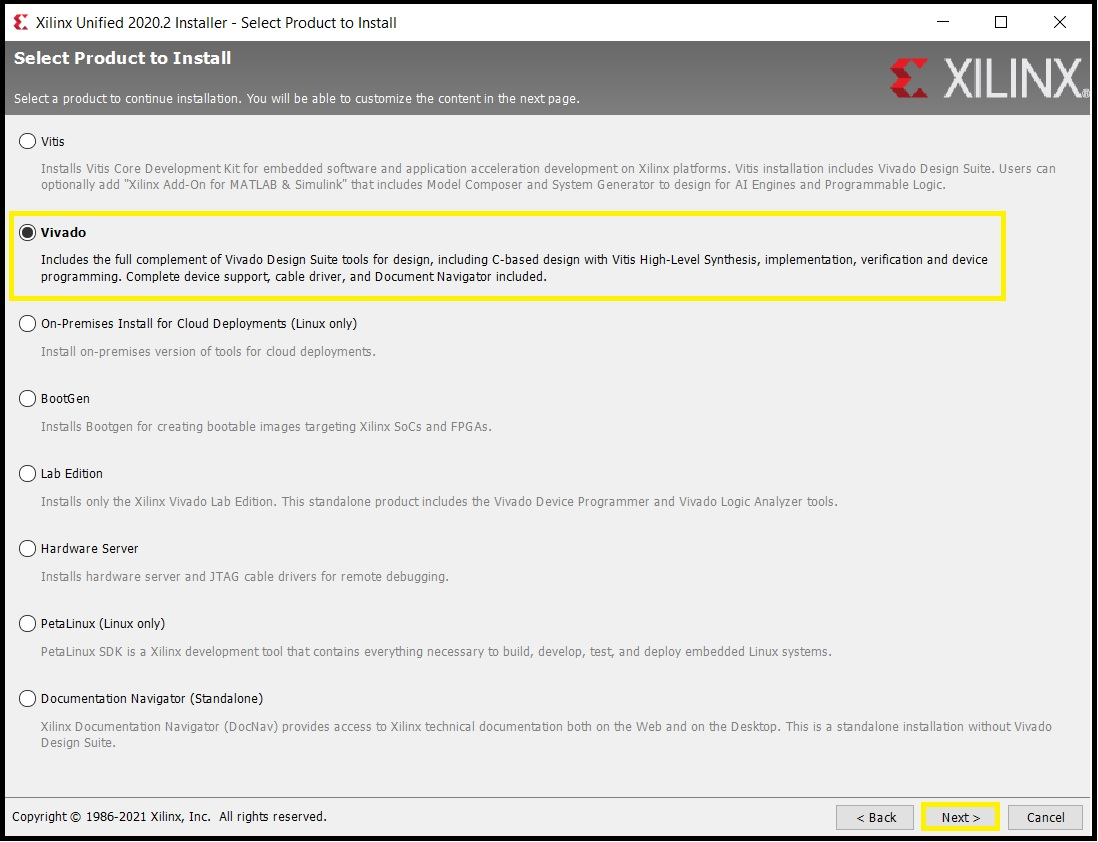
\includegraphics[width=0.7\linewidth]{images/VivadoInstimg010.jpg}
  \end{center}
\end{minipage}

\begin{minipage}{\linewidth}
  Selecteer ``Vivado HL WebPACK'' en klik op ``Next''.
  \\
  \begin{center}
    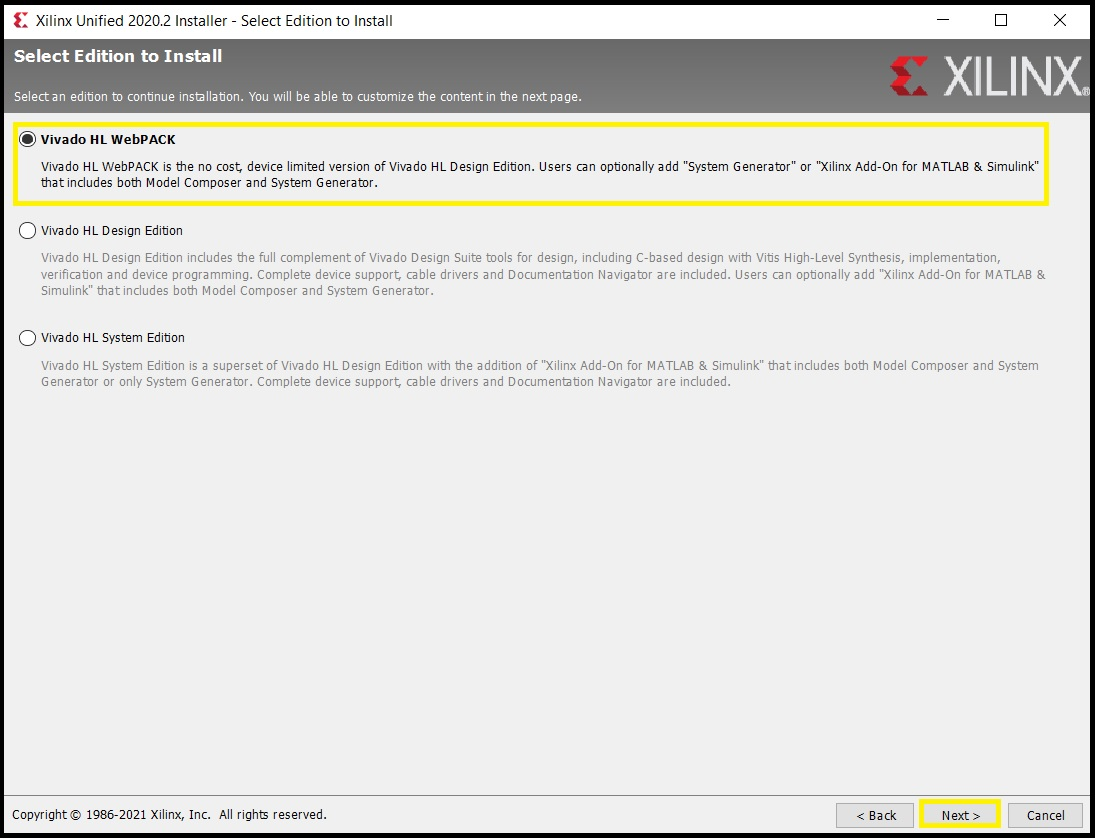
\includegraphics[width=0.7\linewidth]{images/VivadoInstimg011.jpg}
  \end{center}
\end{minipage}

\begin{minipage}{\linewidth}
  Wij raden aan om alleen de apparaten uit de ``\textbf{7 Series}'' te selecteren, omdat onze gekozen FPGA in deze serie valt, en het deselecteren van de andere series bespaart u ongeveer 6 GB aan downloadgrootte. Klik dan op ``Next''.
  \\
  \begin{center}
    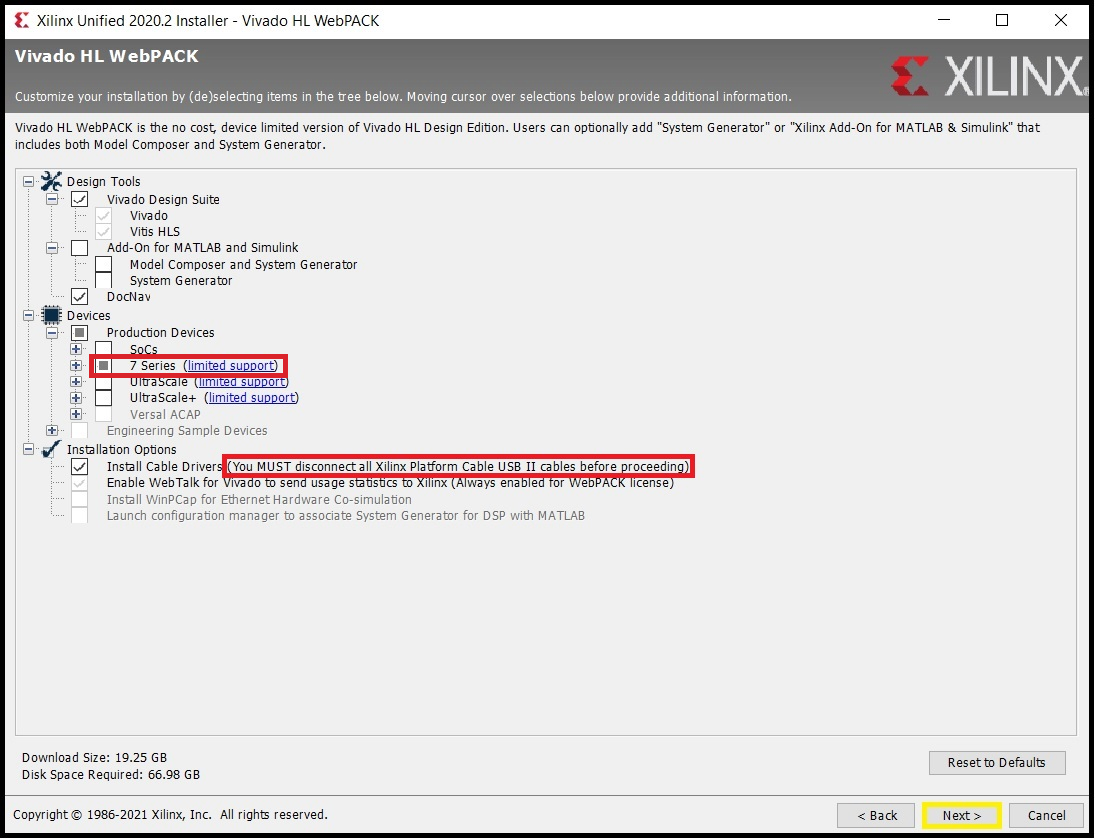
\includegraphics[width=0.7\linewidth]{images/VivadoInstimg012.png}
  \end{center}
  Waarschuwing: zoals gezegd, ontkoppel elke USB-kabel die op uw pc is aangesloten van het Nexys-bord.
\end{minipage}

\begin{minipage}{\linewidth}
  Ga akkoord met alle bepalingen van de eindgebruikerslicentieovereenkomst en de voorwaarden en klik op ``Next''.
  \\
  \begin{center}
    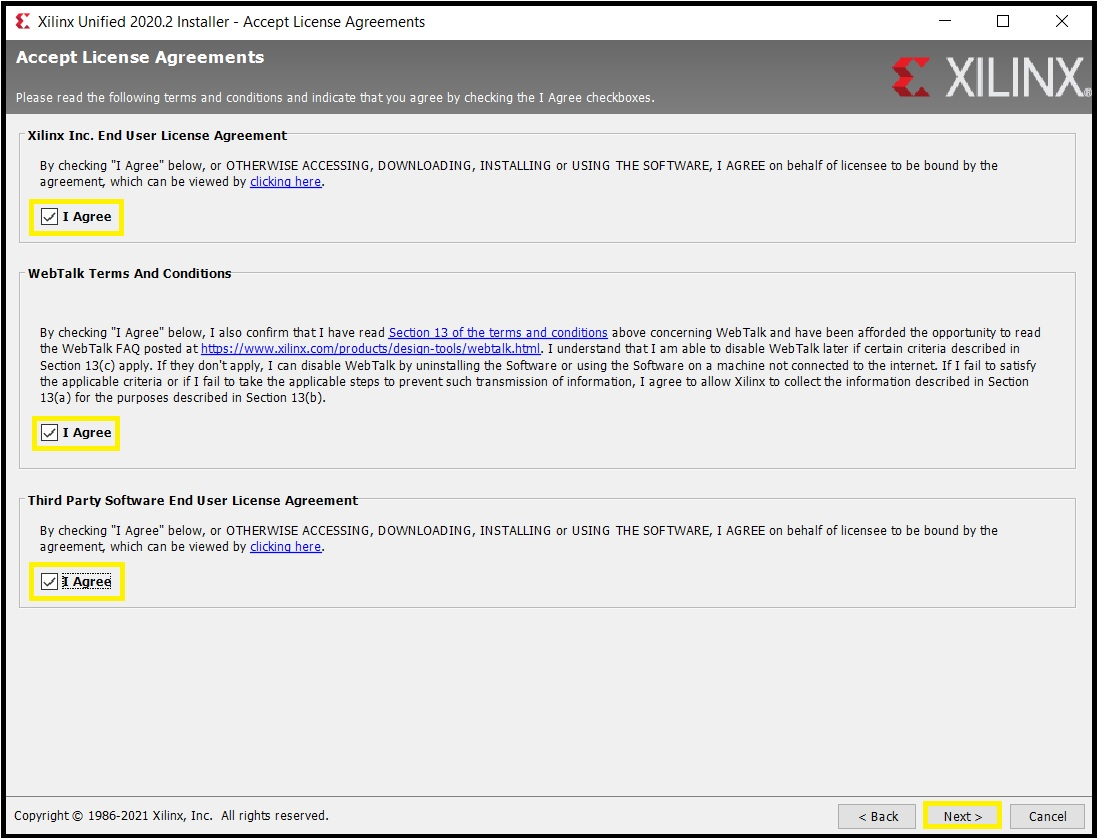
\includegraphics[width=0.7\linewidth]{images/VivadoInstimg013.jpg}
  \end{center}
\end{minipage}

\begin{minipage}{\linewidth}
  Kies de locatie waar u de software wilt installeren en klik op ``Next''.
  \\
  \begin{center}
    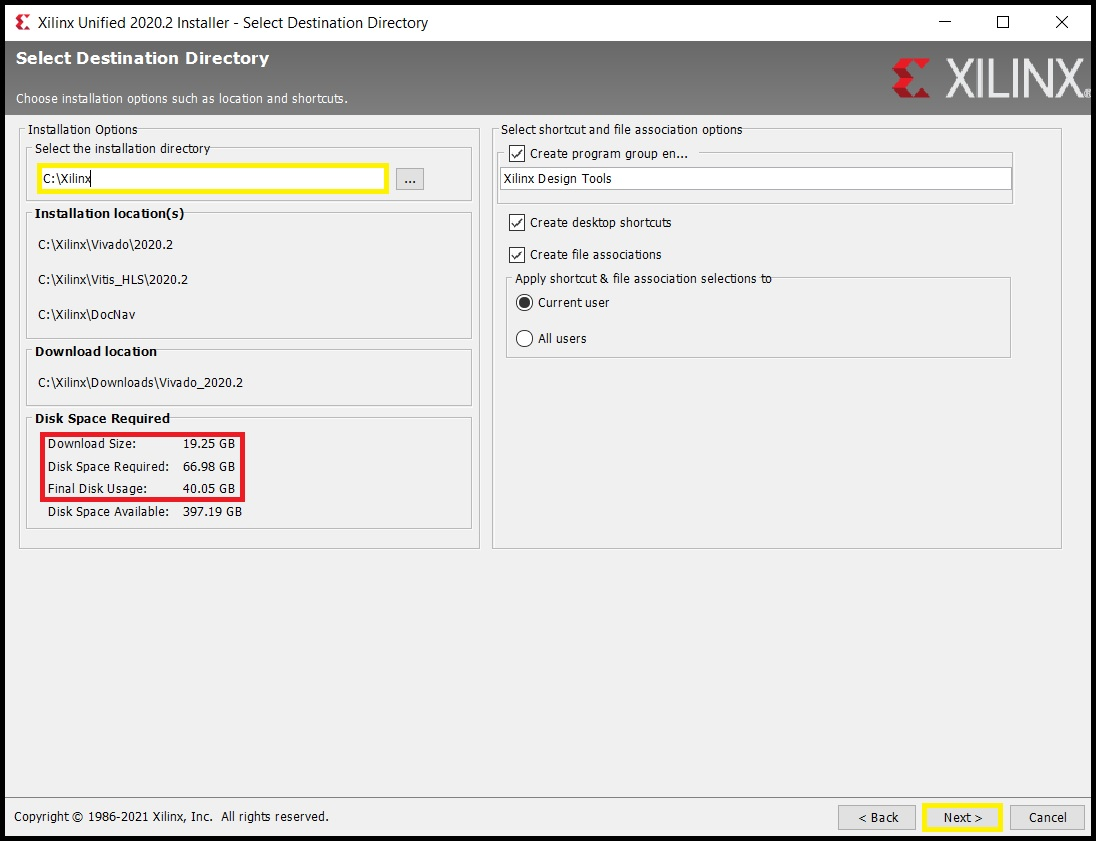
\includegraphics[width=0.7\linewidth]{images/VivadoInstimg014.jpg}
  \end{center}
  Waarschuwing: u staat op het punt om 20 GB aan software te downloaden en u hebt 70 GB nodig om de installatie uit te voeren.
\end{minipage}

\begin{minipage}{\linewidth}
  Klik op ``Yes''.
  \\
  \begin{center}
    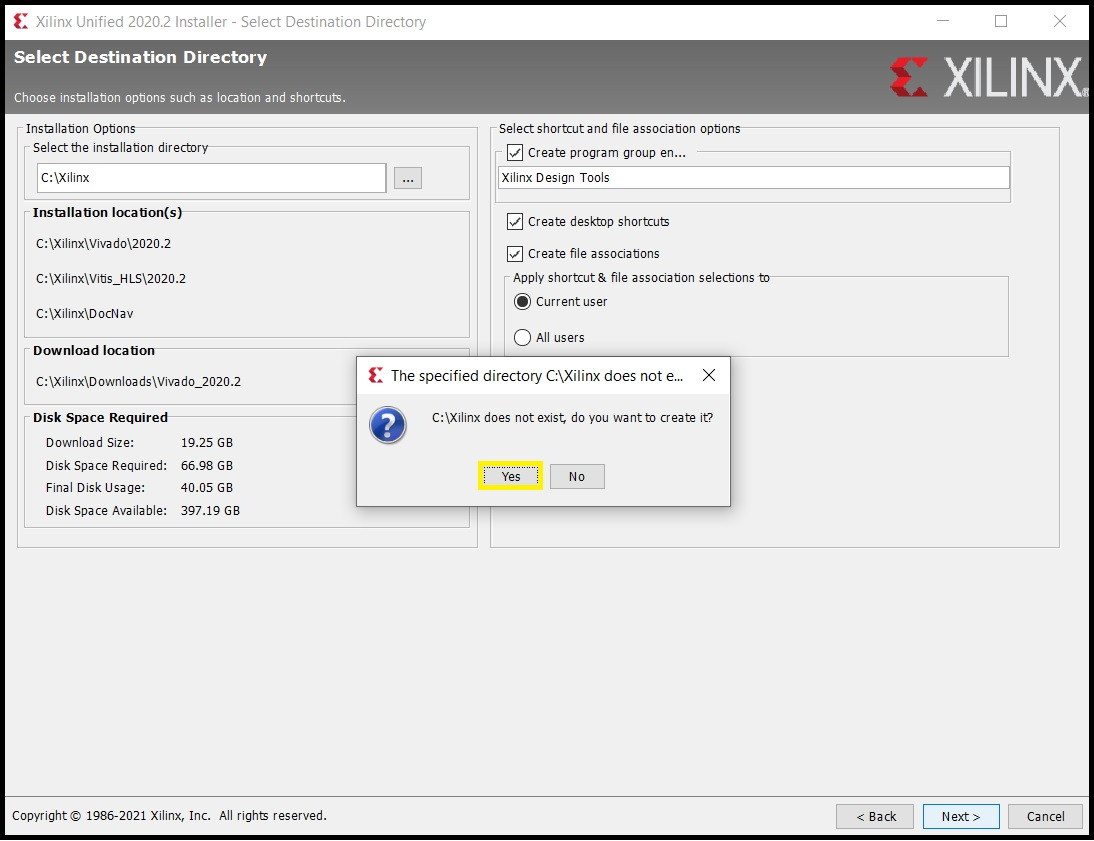
\includegraphics[width=0.7\linewidth]{images/VivadoInstimg015.jpg}
  \end{center}
\end{minipage}

\begin{minipage}{\linewidth}
  Klik op ``Install''.
  \\
  \begin{center}
    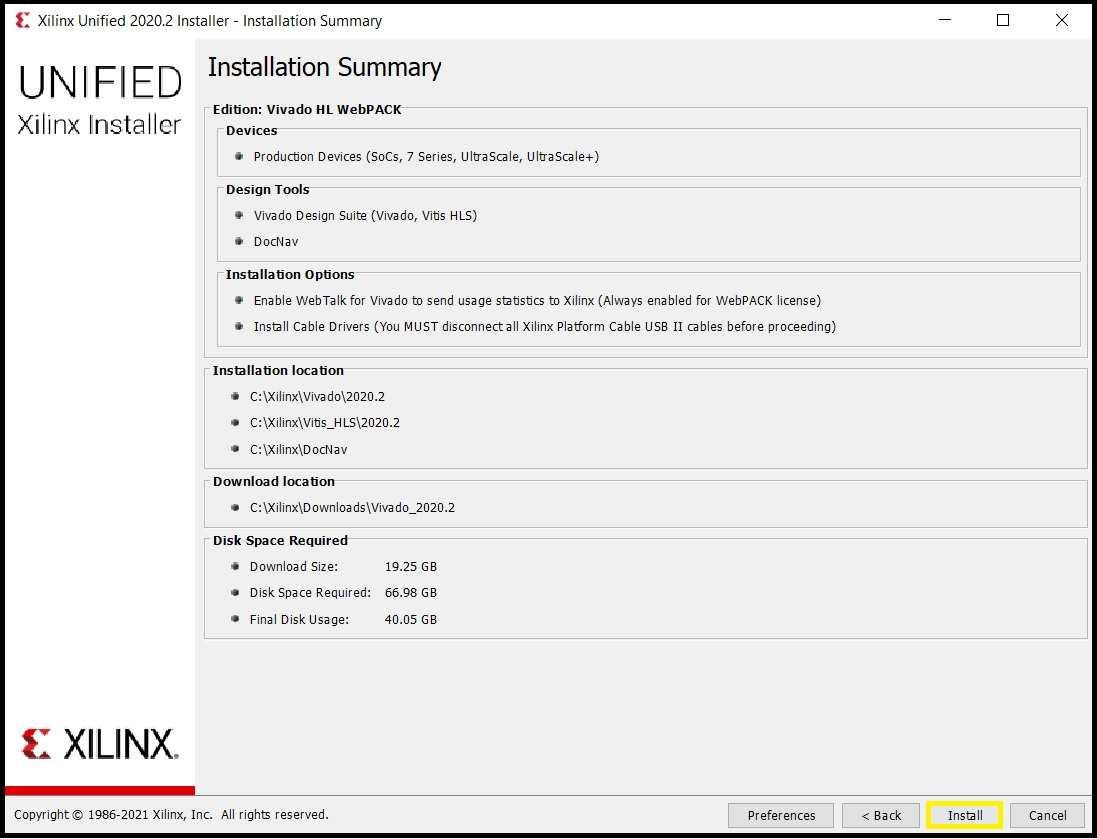
\includegraphics[width=0.7\linewidth]{images/VivadoInstimg016.jpg}
  \end{center}
\end{minipage}

\begin{minipage}{\linewidth}
  Wacht tot de installatie is voltooid. Aan het einde van de installatie wordt u gevraagd of u de Xilinx-apparatensoftware wilt installeren.
  \\
  \begin{center}
    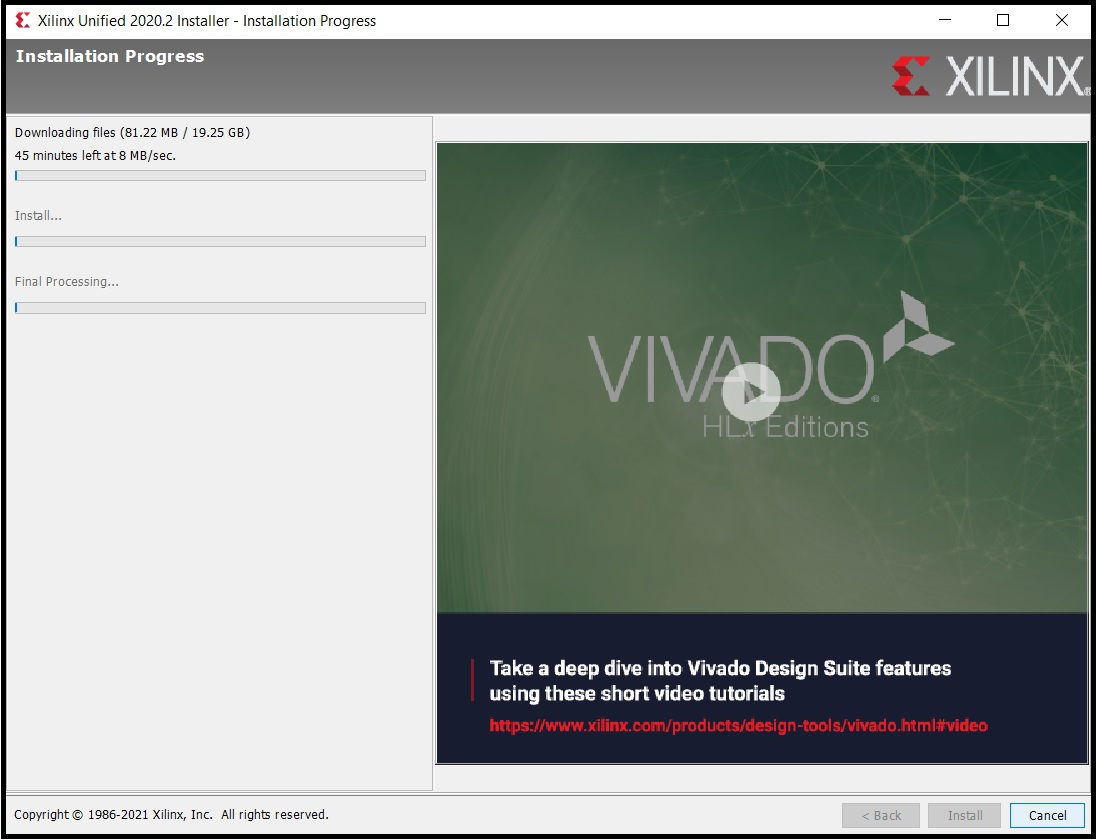
\includegraphics[width=0.7\linewidth]{images/VivadoInstimg017.jpg}
  \end{center}
\end{minipage}

\begin{minipage}{\linewidth}
  Klik op ``Install''.
  \\
  \begin{center}
    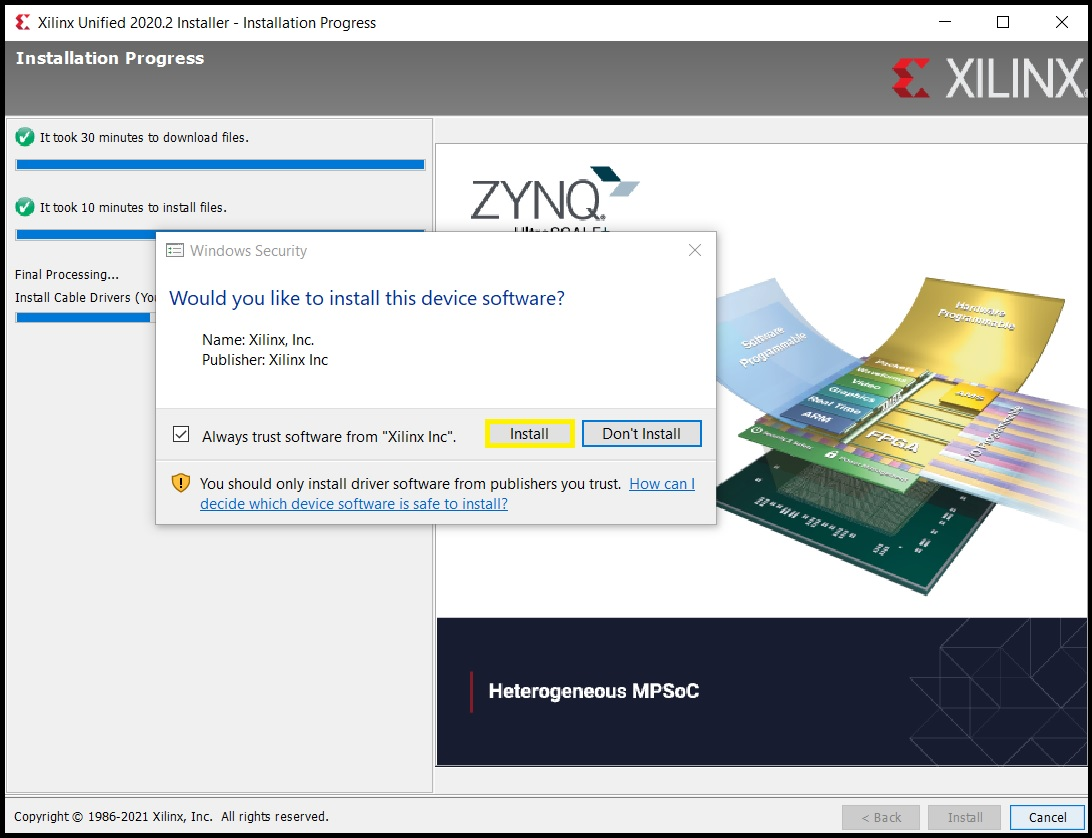
\includegraphics[width=0.7\linewidth]{images/VivadoInstimg018.jpg}
  \end{center}
  Laat de installatie voltooien.
\end{minipage}

\begin{minipage}{\linewidth}
  De installatie is voltooid. Klik op ``OK''.
  \\
  \begin{center}
    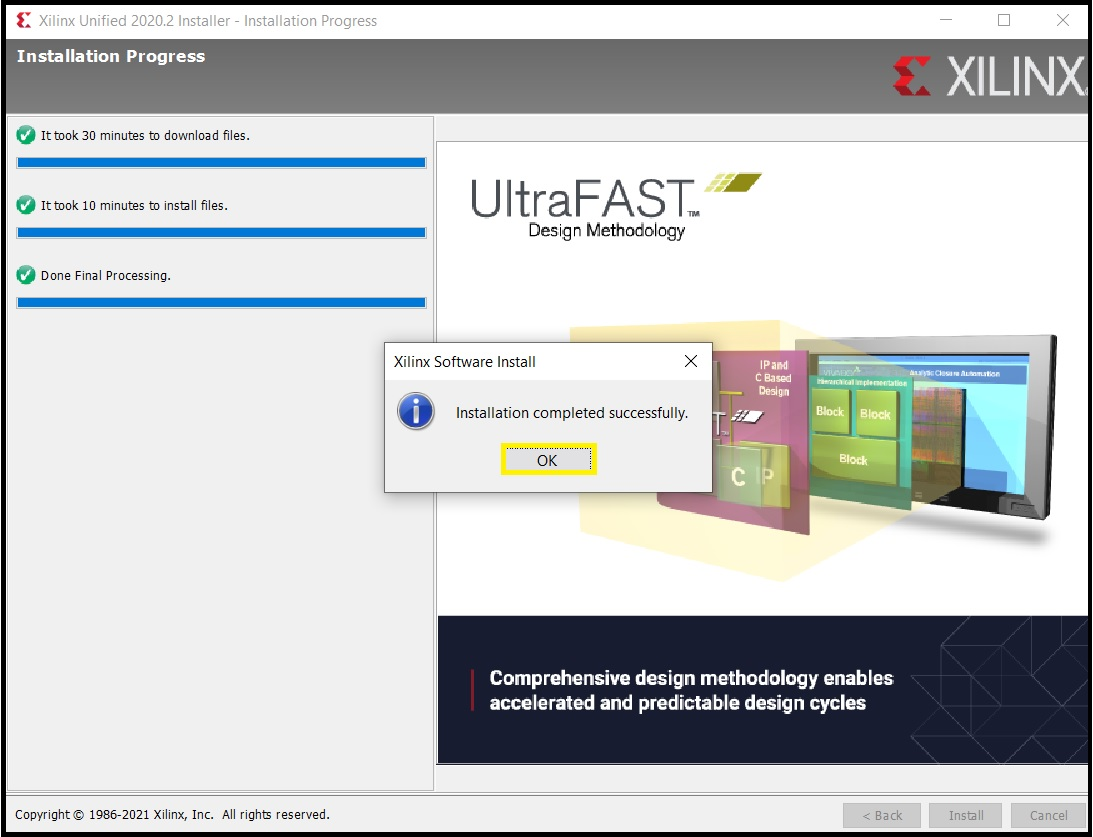
\includegraphics[width=0.7\linewidth]{images/VivadoInstimg019.jpg}
  \end{center}
\end{minipage}

\begin{minipage}{\linewidth}
  Op uw bureaublad verschijnen nu de volgende pictogrammen:
  \\
  \begin{center}
    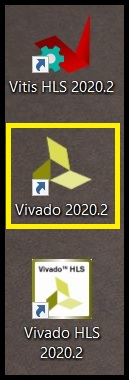
\includegraphics[width=0.2\linewidth]{images/VivadoInstimg020.jpg}
  \end{center}
  Let op: Ubuntu-gebruikers moeten mogelijk een ontbrekende afhankelijkheid installeren met: {\tt sudo apt install libtinfo5}
\end{minipage}

\begin{minipage}{\linewidth}
  Start Vivado 2020.2
  \\
  \begin{center}
    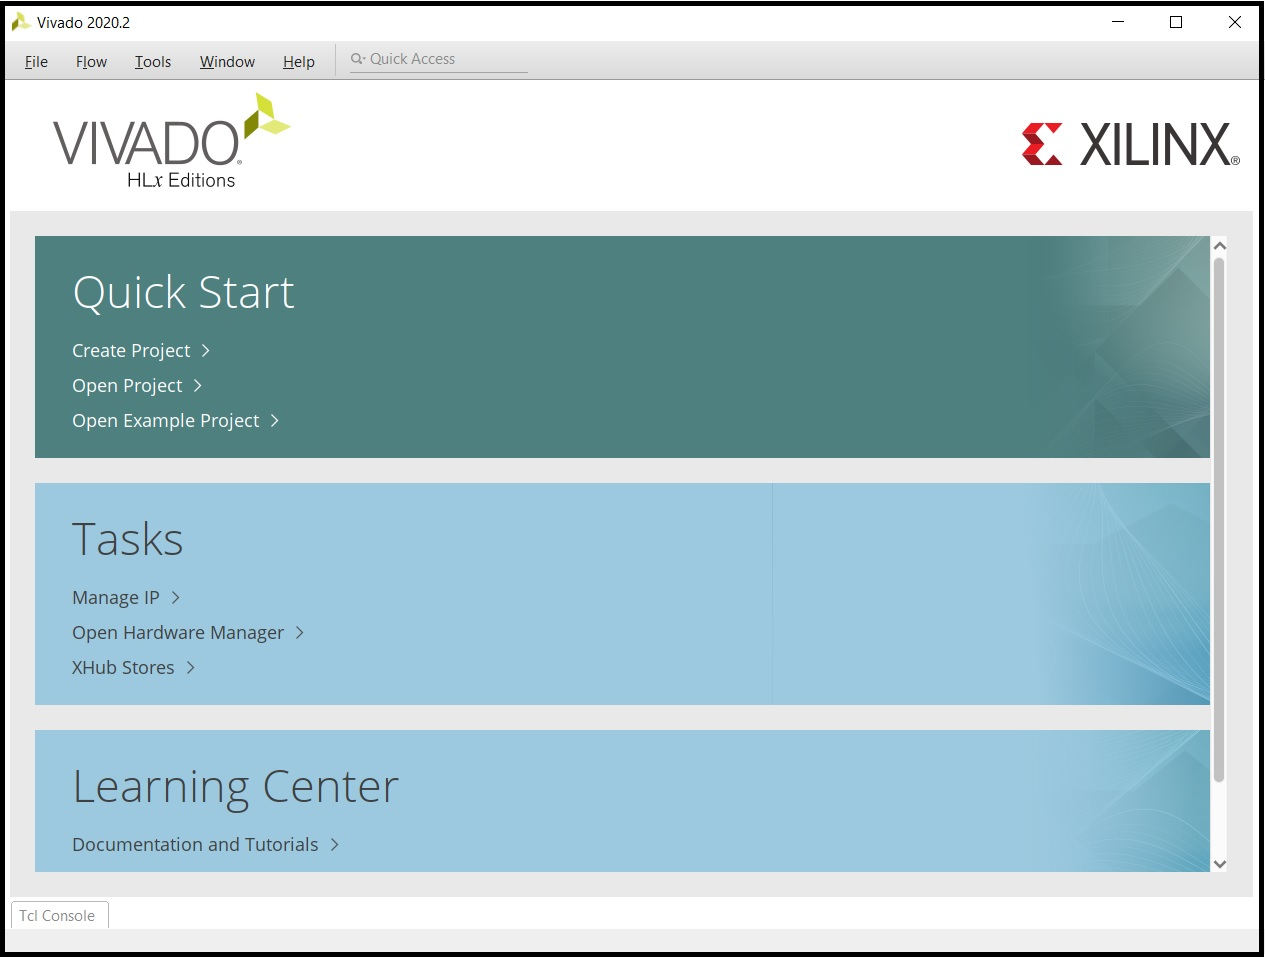
\includegraphics[width=0.7\linewidth]{images/VivadoInstimg021.jpg}
  \end{center}
\end{minipage}

\begin{minipage}{\linewidth}
  Klik op ``Help''->``Obtain a licence Key''.
  \\
  \begin{center}
    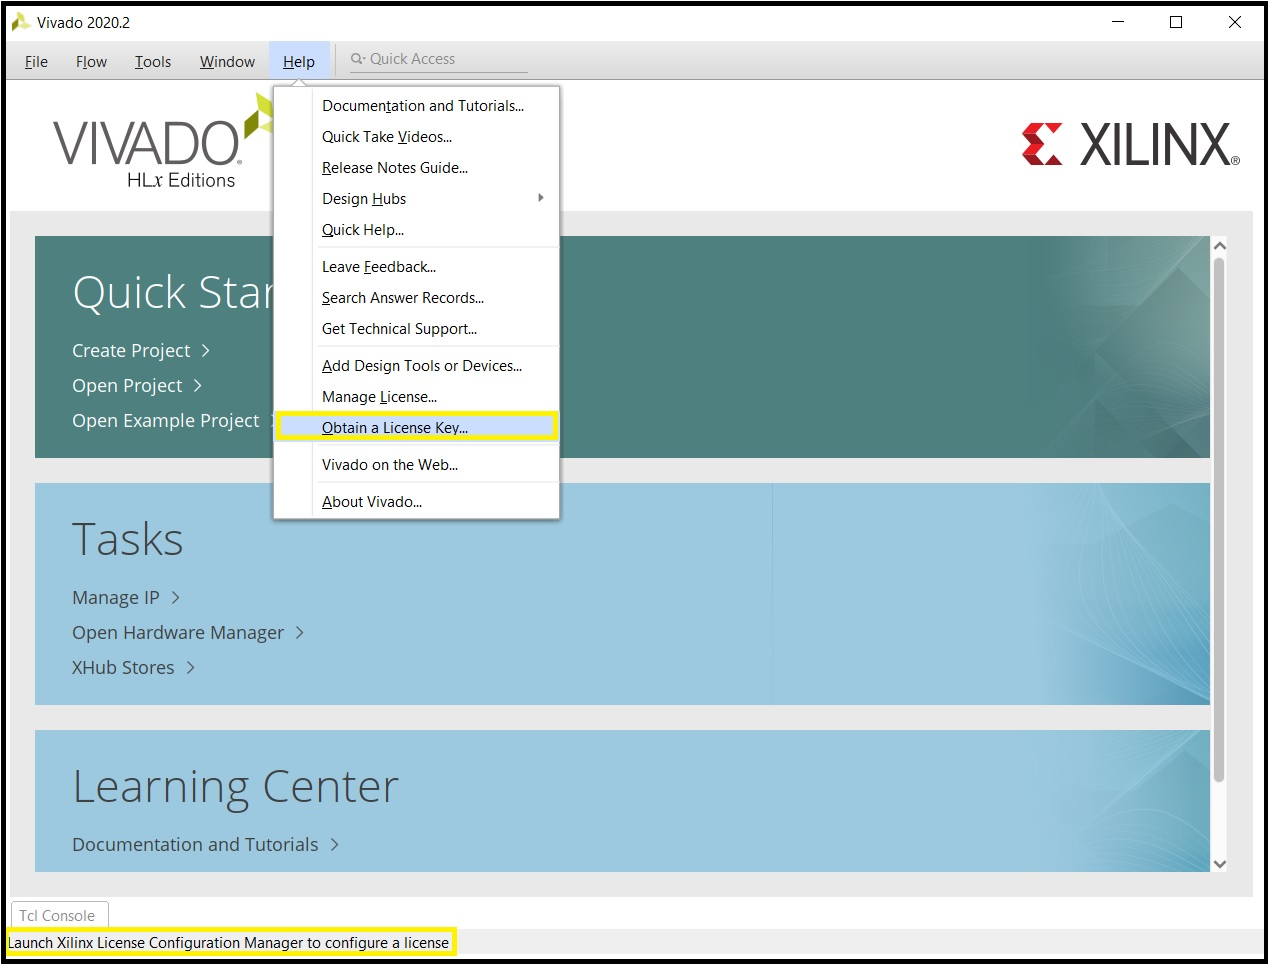
\includegraphics[width=0.7\linewidth]{images/VivadoInstimg022.jpg}
  \end{center}
\end{minipage}

\begin{minipage}{\linewidth}
  Hiermee opent u de Vivado-licentiemanager. \\
  \\
  Selecteer ``Get Free ISE WebPACK, ISE/Vivado IP or PetaLinux Licenses'' \\
  \\
  Klik op ``Connect Now''.
  \\
  \begin{center}
    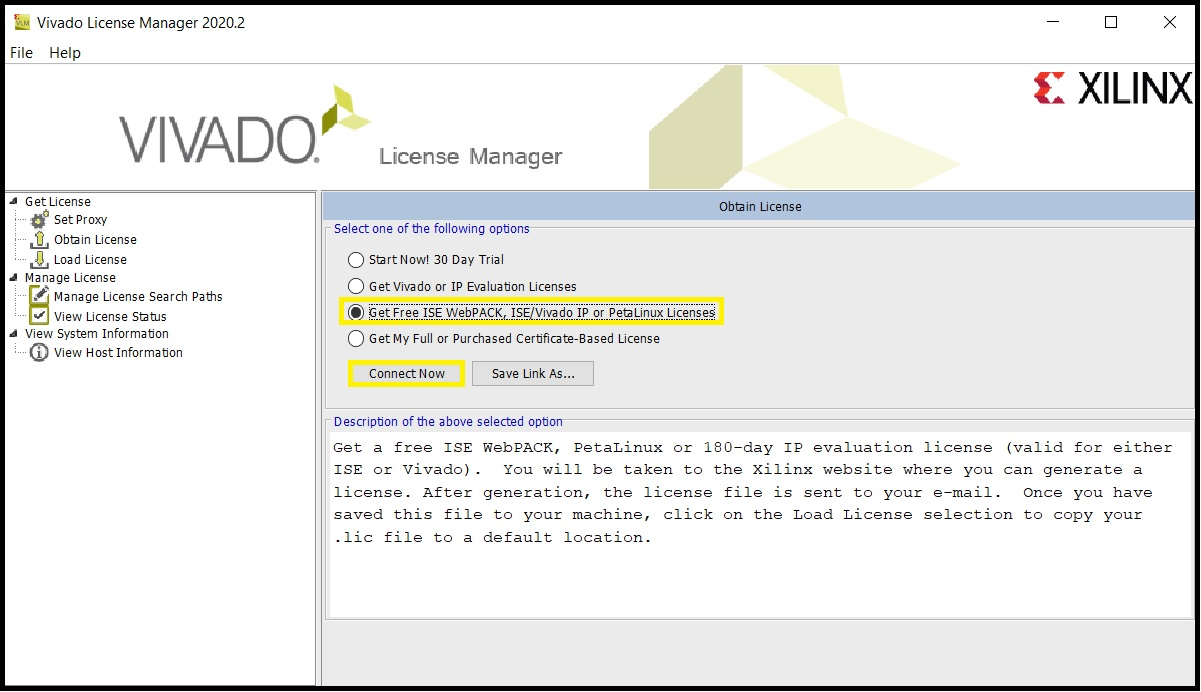
\includegraphics[width=\linewidth]{images/VivadoInstimg023.jpg}
  \end{center}
\end{minipage}

\begin{minipage}{\linewidth}
  Verbind met het gebruikersaccount dat u hebt aangemaakt om de Vivado-software te kunnen downloaden. Als u nog niet op de website van Xilinx was ingelogd, wordt u naar de hoofdpagina geleid. Keer terug naar de licentiemanager (die niet is gesloten).
  \\
  \begin{center}
    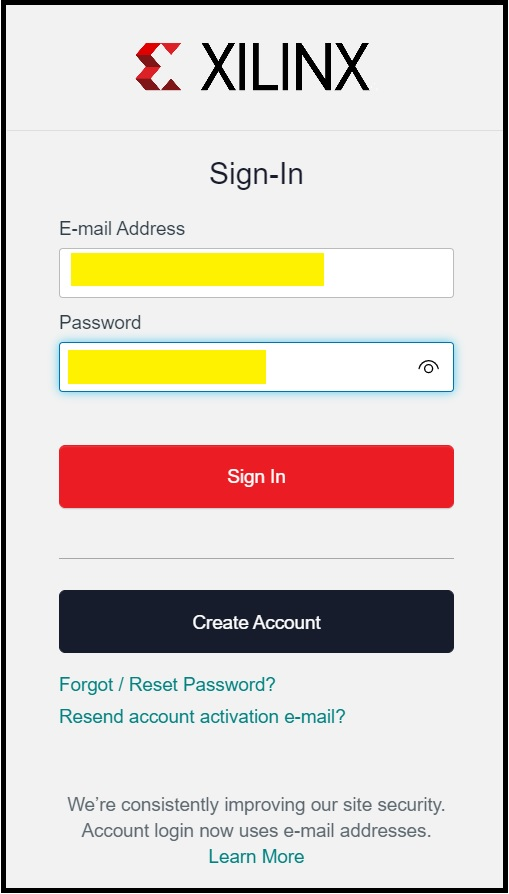
\includegraphics[width=0.3\linewidth]{images/VivadoInstimg024.jpg}
  \end{center}
\end{minipage}

\begin{minipage}{\linewidth}
  Klik opnieuw op ``Connect Now'' (controleer of ``Get Free ISE WebPACK, ISE/Vivado IP or PetaLinux Licenses'' nog steeds is geselecteerd).
  \\
  \begin{center}
    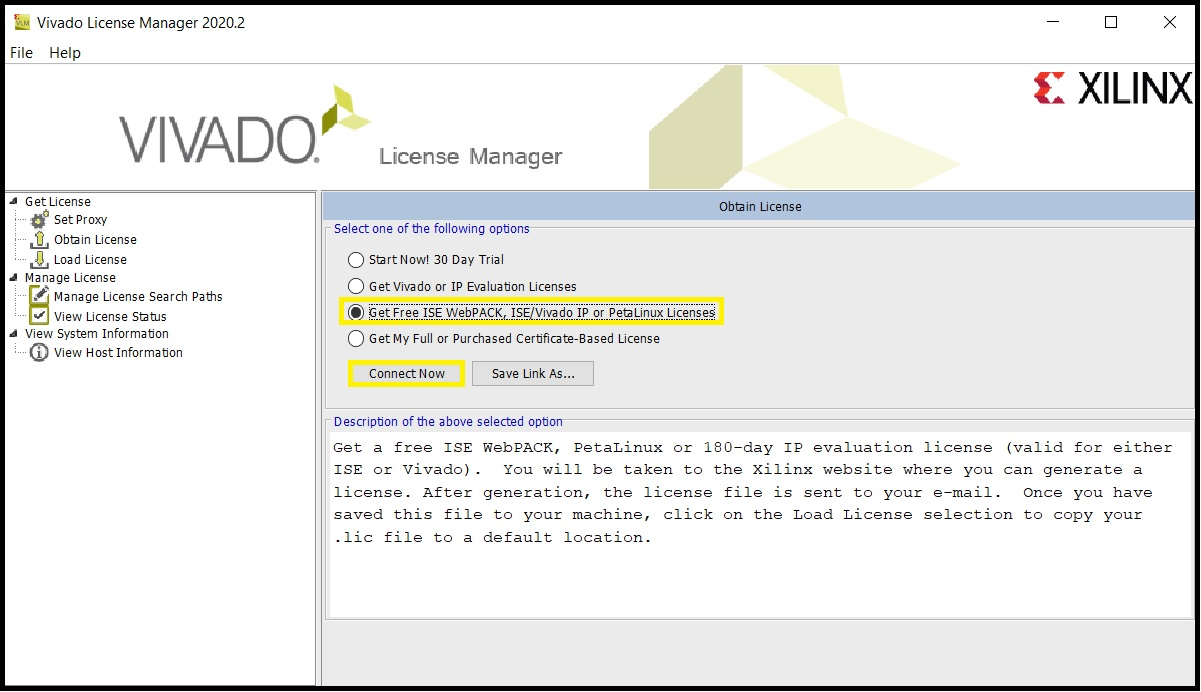
\includegraphics[width=\linewidth]{images/VivadoInstimg023.jpg}
  \end{center}
\end{minipage}

\begin{minipage}{\linewidth}
  Vervolgens registreert u uw persoonlijke gegevens op de Vivado-website en klikt u op ``Next''.
  \\
  \begin{center}
    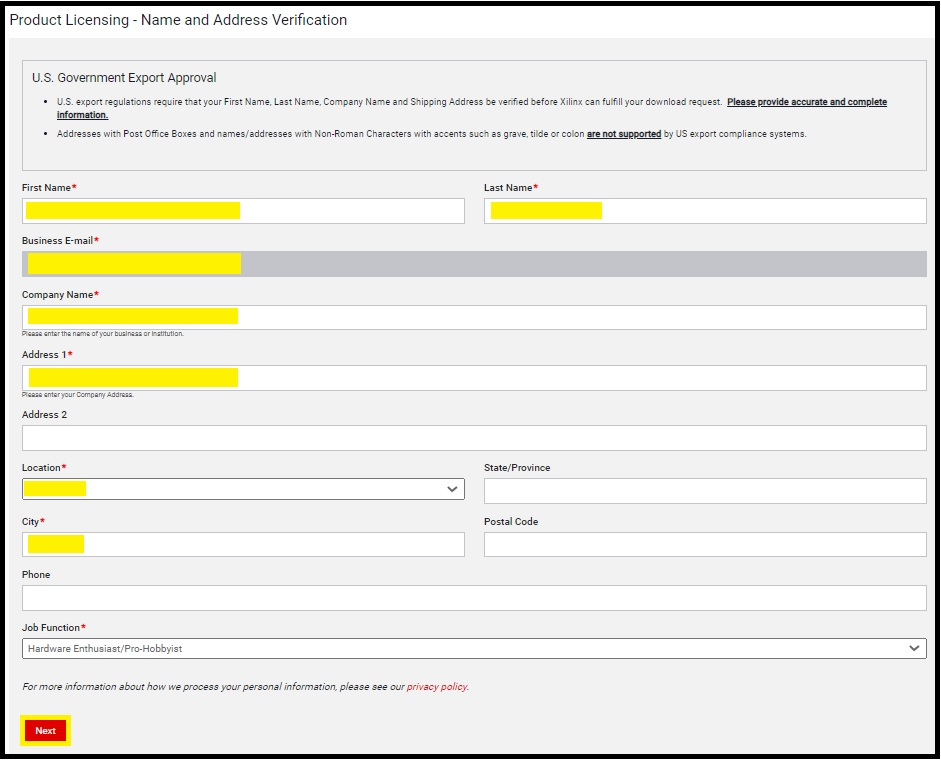
\includegraphics[width=0.7\linewidth]{images/VivadoInstimg025.jpg}
  \end{center}
\end{minipage}


\begin{minipage}{\linewidth}
Selecteer ``ISE WebPACK Licence'' en ``Vivado Design Suite: HL WebPACK 2015 and Earlier License'' \\
\\
Klik vervolgens op ``Generate Node-Locked Licence''.
\\
\begin{center}
  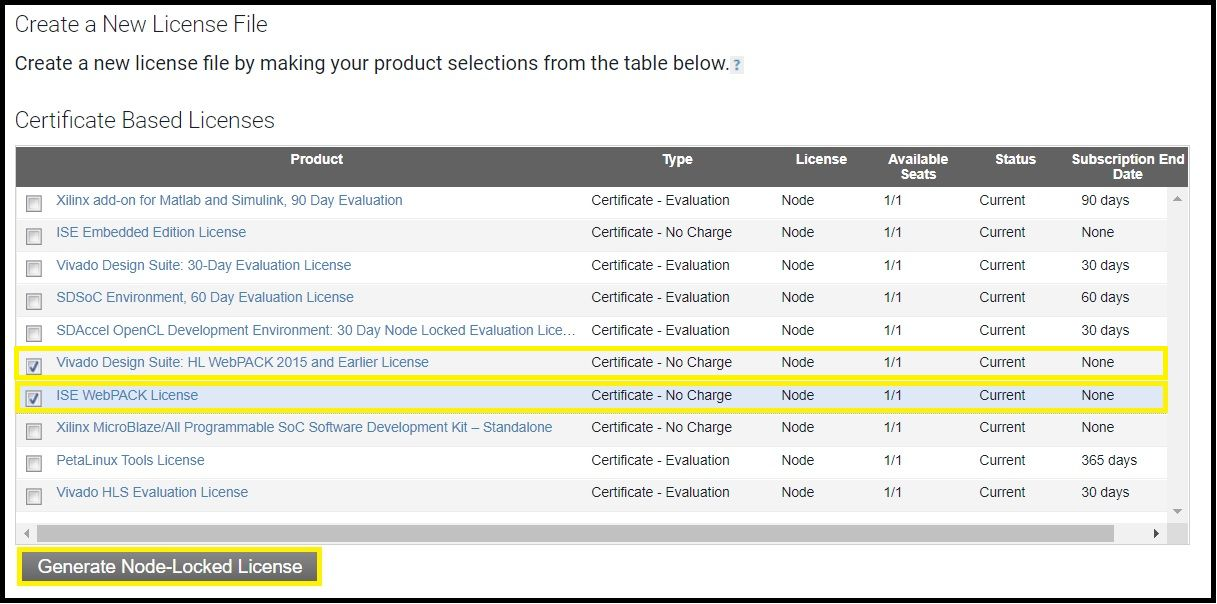
\includegraphics[width=\linewidth]{images/VivadoInstimg026.jpg}
\end{center}
\end{minipage}

\begin{minipage}{\linewidth}
  Klik op ``Next''.
  \\
  \begin{center}
    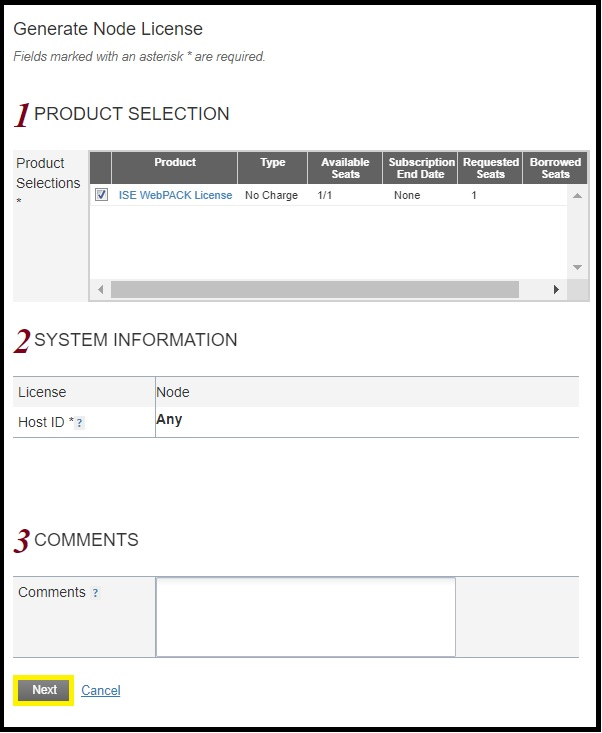
\includegraphics[width=0.5\linewidth]{images/VivadoInstimg027.jpg}
  \end{center}
\end{minipage}

\begin{minipage}{\linewidth}
  Klik op ``Next''.
  \\
  \begin{center}
    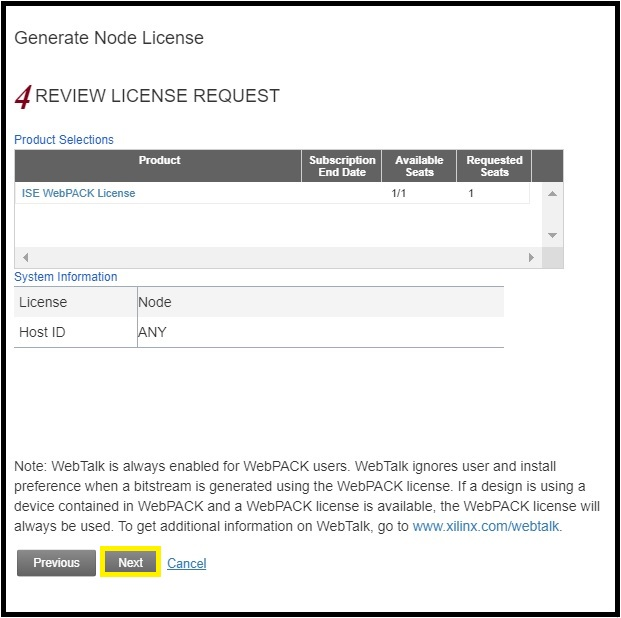
\includegraphics[width=0.5\linewidth]{images/VivadoInstimg028.jpg}
  \end{center}
\end{minipage}


\begin{minipage}{\linewidth}
  Controleer uw e-mail: u hebt een e-mail ontvangen van Xilinx, Inc. met een licentiebestand met de naam ``Xilinc.lic'' als bijlage. \\
  \\
  Sla dit bestand op uw computer op en bewaar het op een veilige plaats.
  \\
  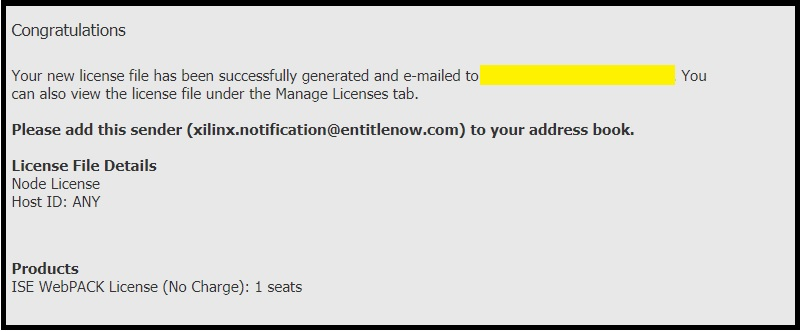
\includegraphics[width=\linewidth]{images/VivadoInstimg029.jpg}
\end{minipage}

\begin{minipage}{\linewidth}
  Ga terug naar de licentiemanager (die nog steeds actief is). \\
  \\
  Selecteer ``Load License'' en klik op ``Copy License''.
  \\
  \begin{center}
    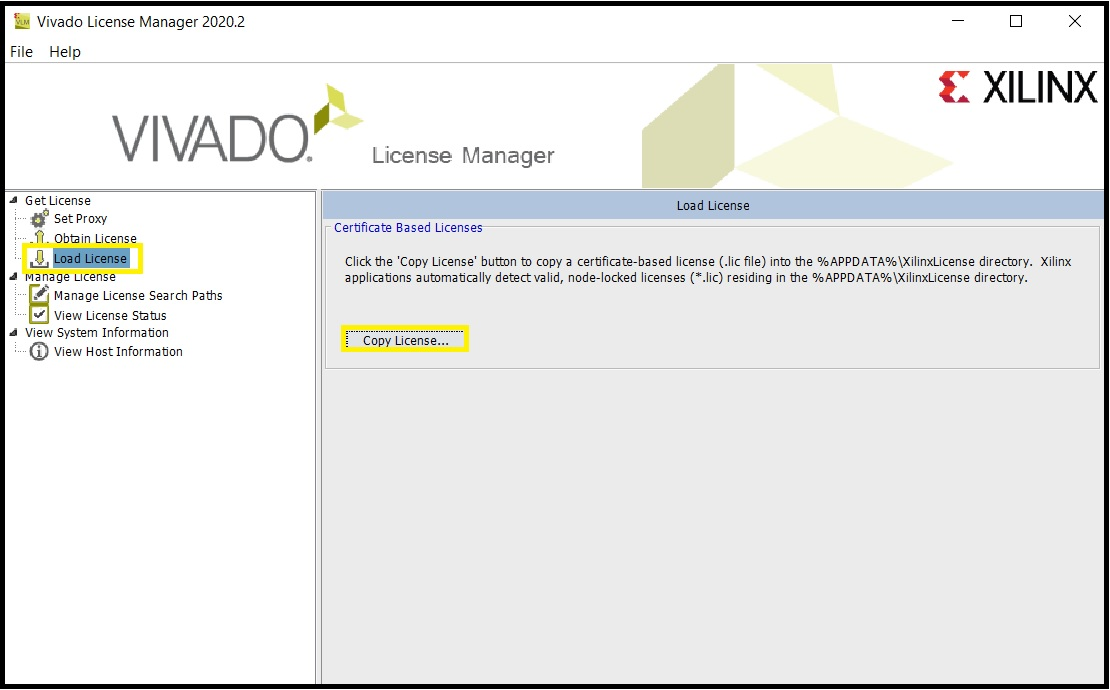
\includegraphics[width=0.8\linewidth]{images/VivadoInstimg030.jpg}
  \end{center}
\end{minipage}

\begin{minipage}{\linewidth}
  Blader naar de locatie waar u het bestand ``Xilinc.lic'' heeft opgeslagen, selecteer het en klik op ``Open''.
  \\
  \begin{center}
    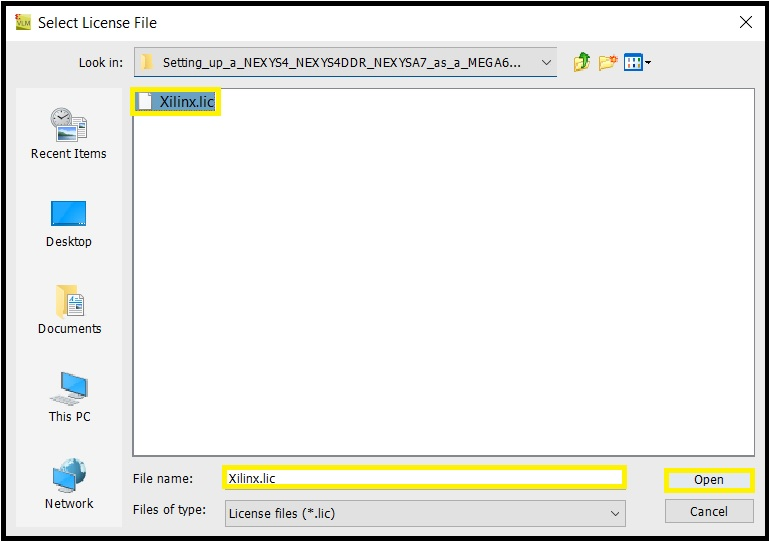
\includegraphics[width=0.7\linewidth]{images/VivadoInstimg031.jpg}
  \end{center}
\end{minipage}

\begin{minipage}{\linewidth}
  Klik op ``OK'' en sluit de Vivado-licentiemanager.
  \\
  \begin{center}
    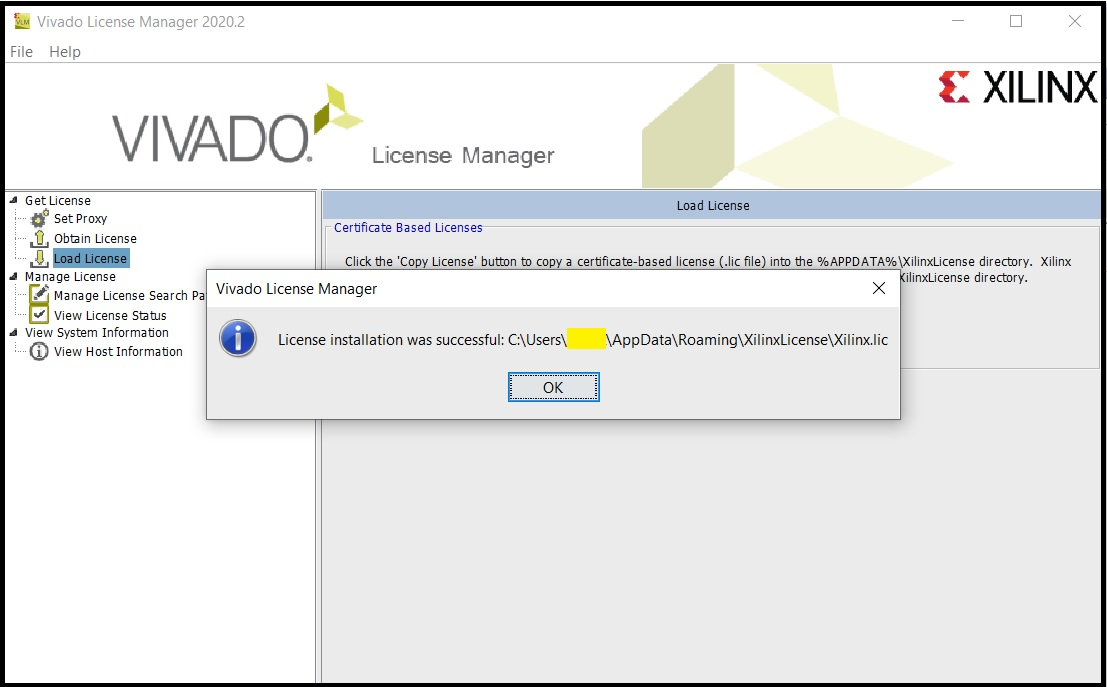
\includegraphics[width=0.7\linewidth]{images/VivadoInstimg032.jpg}
  \end{center}

  Uw Vivado-software is geregistreerd en u kunt deze nu gebruiken.
\end{minipage}

\section{De FTDI-stuurprogramma's installeren}

De FTDI-drivers zijn nodig om uw PC te laten communiceren met de JTAG-poort en de seriële communicatiepoort van de hardware (merk op dat de enkele fysieke USB-verbinding met uw PC feitelijk deze twee poorten aanbiedt).

\subsection{Linux-drivers}

Gebruikers van Linux melden dat zij de FTDI-drivers standaard in hun Linux-distributie aangetroffen hebben, terwijl anderen aangeven dat het volgende extra commando na de installatie van Vivado uitgevoerd moet worden:

cd /opt/Xilinx/Vivado/2018.3/data/xicom/cable\_drivers/lin64/install\_script/install\_drivers \\sudo ./install\_drivers

\subsection{Windows-drivers}

Download het volgende archief om de drivers te installeren:

\begin{itemize}
  \item \url{https://ftdichip.com/wp-content/uploads/2021/08/CDM212364_Setup.zip}
\end{itemize}

Pak het bestand \textbf{CDM212364\_Setup.zip} uit; u verkrijgt het bestand \textbf{CDM212364\_Setup.exe}.

\textcolor{red}{\underline{Waarschuwing}: \\Voordat u de drivers installeert, moet u de Nexys4-plaat uitschakelen en de USB-kabel loskoppelen van de PC.}

\begin{minipage}{\linewidth}
  Controleer welke apparaten er voor de installatie al aanwezig zijn:
  \\
  \begin{center}
    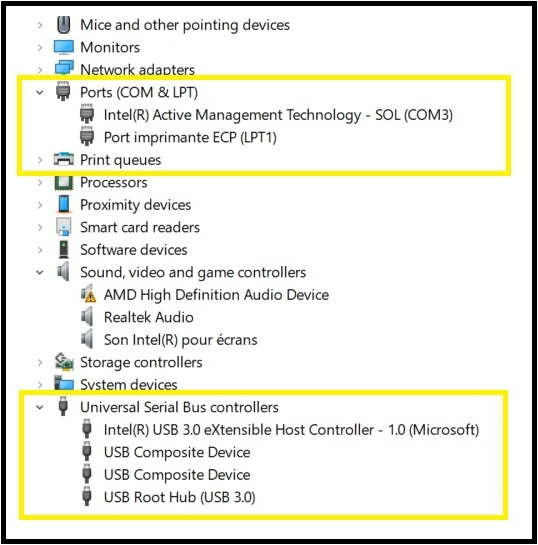
\includegraphics[width=0.6\linewidth]{images/img001_install_drivers_00.jpg}
  \end{center}
\end{minipage}

\begin{minipage}{\linewidth}
  Voer het bestand CDM212364\_Setup.exe uit als administrator:
  \\
  \begin{center}
    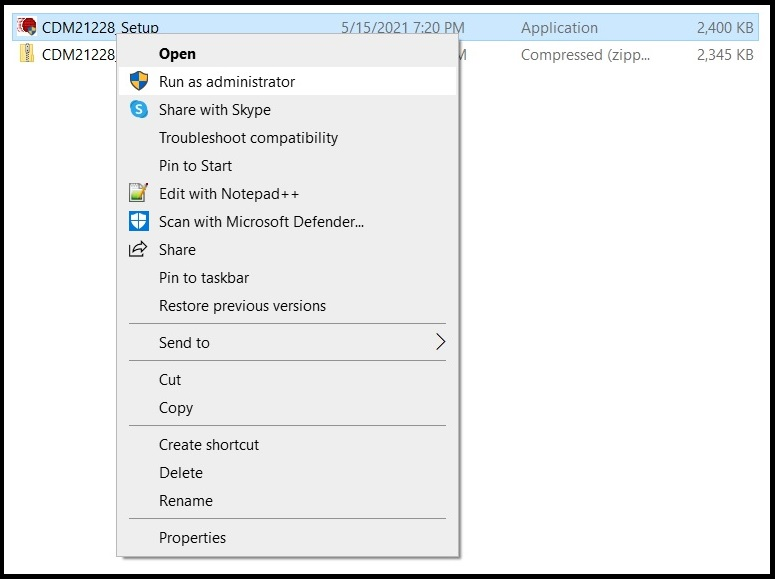
\includegraphics[width=0.6\linewidth]{images/img001_install_drivers_01.jpg}
  \end{center}
\end{minipage}

Bevestig dat u het programma wilt uitvoeren.

\begin{minipage}{\linewidth}
  Klik op ``Extract''.
  \\
  \begin{center}
    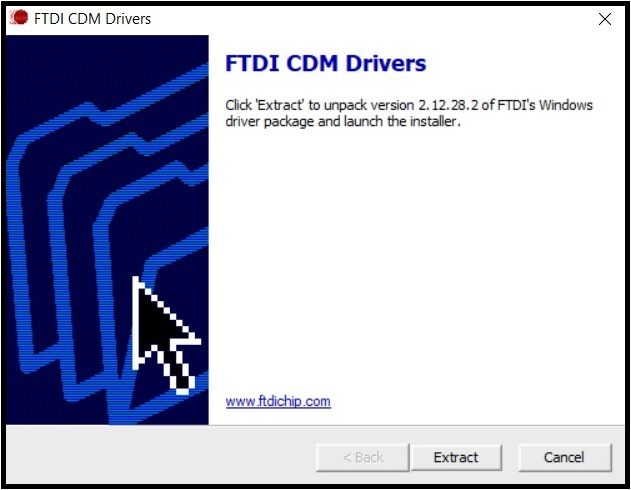
\includegraphics[width=0.6\linewidth]{images/img001_install_drivers_02.jpg}
  \end{center}
\end{minipage}

\begin{minipage}{\linewidth}
  Klik op ``Next >''.
  \\
  \begin{center}
    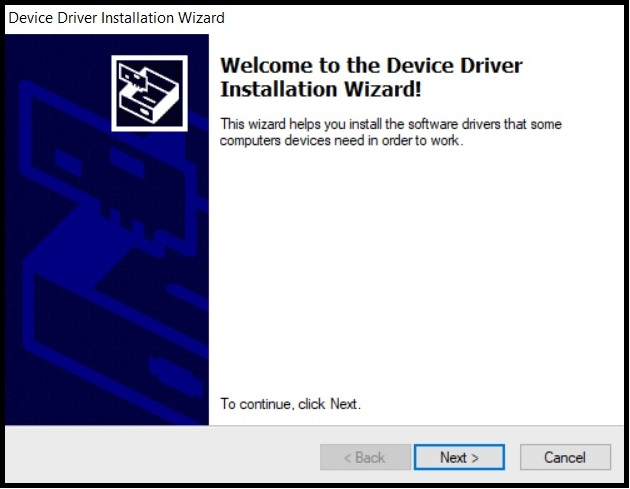
\includegraphics[width=0.6\linewidth]{images/img001_install_drivers_03.jpg}
  \end{center}
\end{minipage}

\begin{minipage}{\linewidth}
  Aanvaard de overeenkomst en klik op ``Next >''.
  \\
  \begin{center}
    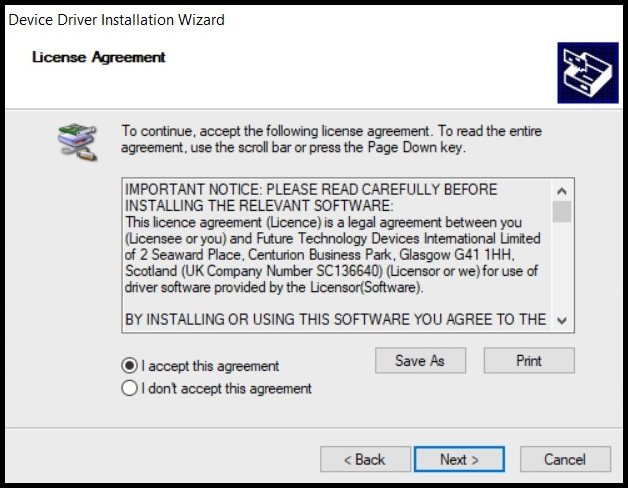
\includegraphics[width=0.6\linewidth]{images/img001_install_drivers_04.jpg}
  \end{center}
\end{minipage}

De installatie van de drivers wordt gestart.

\begin{minipage}{\linewidth}
  Klik op ``Finish''.
  \\
  \begin{center}
    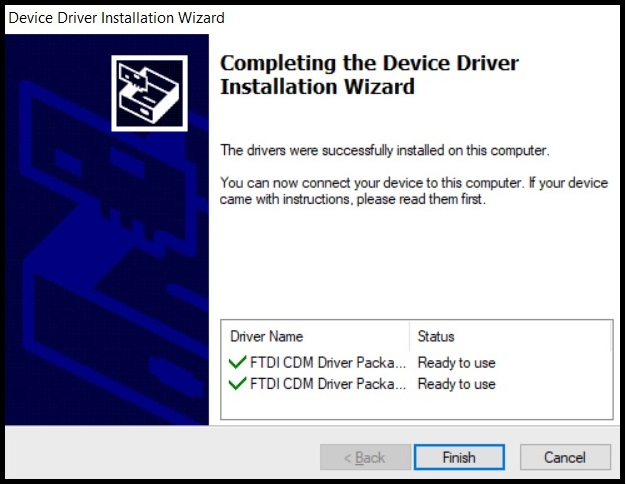
\includegraphics[width=0.6\linewidth]{images/img001_install_drivers_05.jpg}
  \end{center}
\end{minipage}

Sluit de USB-kabel aan op een USB-poort op de PC \textcolor{red}{zonder de Nexys4-plaat in te schakelen}.

Het aansluiten van de USB-kabel veroorzaakt het verschijnen van nieuwe apparaten.

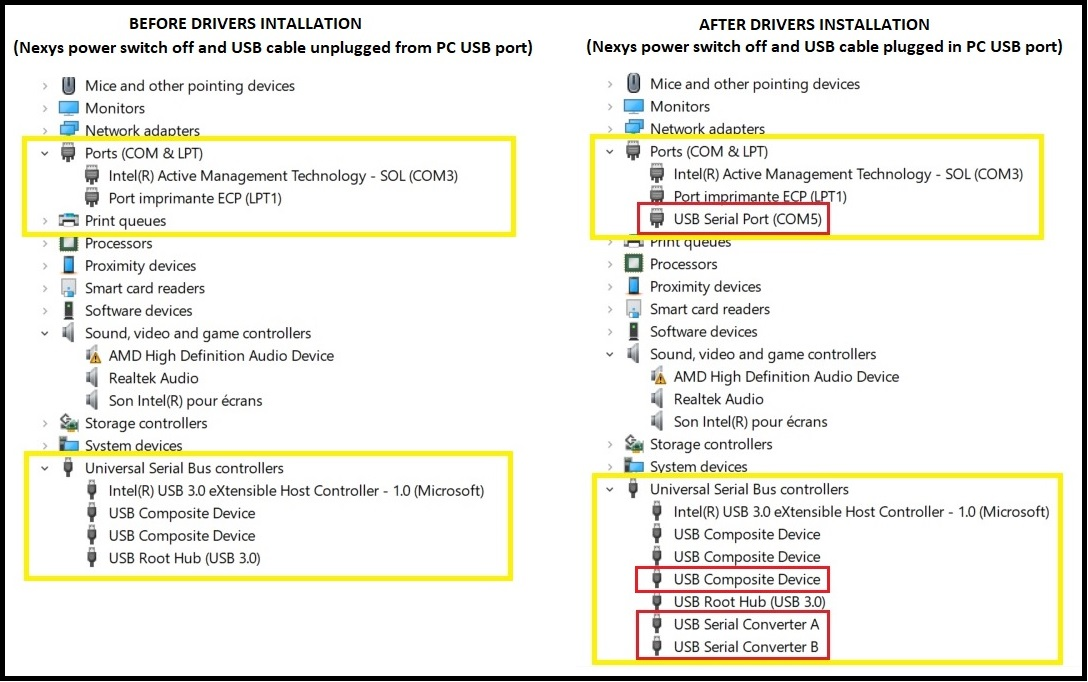
\includegraphics[width=\linewidth]{images/img001_install_drivers_07.jpg}

\begin{itemize}
  \item Er is een extra COM-poort geïnstalleerd: \textcolor{red}{dit is de COM-poort die gebruikt wordt om met de Nexys4-plaat te communiceren.}  \item Er is een extra USB-samengesteld apparaat geïnstalleerd.  \item Er zijn twee USB-serieel-omzetters geïnstalleerd.
\end{itemize}

Op dit moment is de Nexys4-plaat nog niet van stroom voorzien.

Voor meer informatie over de geïnstalleerde drivers kunt u de bijbehorende documentatie downloaden:

\begin{itemize}
  \item \url{https://ftdichip.com/wp-content/uploads/2020/08/AN\_396-FTDI-Drivers-Installation-Guide-for-Windows-10.pdf}
  \item \url{https://ftdichip.com/wp-content/uploads/2021/01/AN\_119\_FTDI\_Drivers\_Installation\_Guide\_for\_Windows7.pdf}
\end{itemize}

\section{De hoofd-FPGA flashen met Vivado}
\label{sec:mainfpgaflashing}

Ter verduidelijking: wanneer wij spreken over het ``flashen van de FPGA'', bedoelen wij in feite het flashen van het QSPI-flashgeheugen waarvan de FPGA bij het opstarten gebruikmaakt om de bitstream snel te laden.

De afbeelding hieronder toont twee veelgebruikte manieren waarop de FPGA bij het opstarten een bitstream kan laden:

\begin{center}
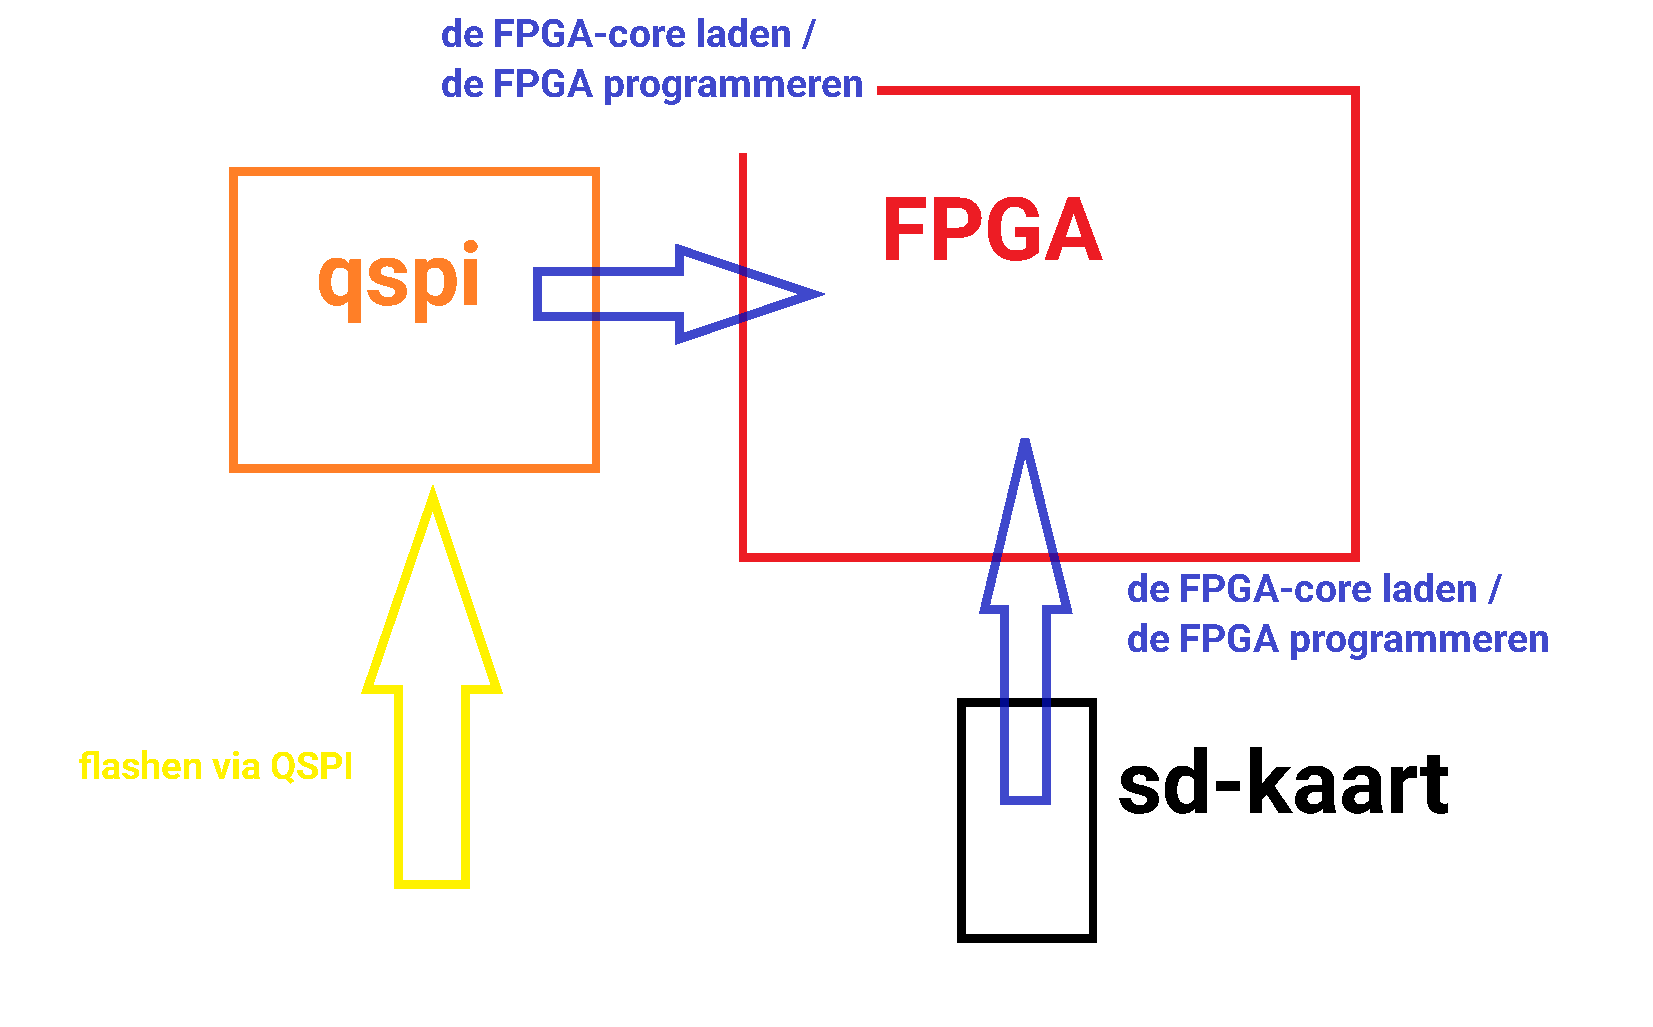
\includegraphics[width=0.8\linewidth]{dutch/images/flashing_fpga.pdf}
\end{center}

\begin{itemize}
  \item We kunnen eerst een bitstream-/core-bestand op het QSPI-flashgeheugen flashen, waarna de FPGA dit bij het opstarten snel kan laden. Het flashen van het QSPI is tamelijk traag, maar het voordeel van een korte opstarttijd is een duidelijke meerwaarde.  \item Gebruikers van een Nexys-plaat kunnen een bitstream-bestand op hun SD-kaart plaatsen en de FPGA dit (enigszins langzamer) bij het opstarten vanaf daar laten laden. Hierdoor kunnen bitstreams snel gewisseld of bijgewerkt worden zonder een TE0790-03 JTAG-programmeermodule. Deze functionaliteit is echter voor later gepland voor de MEGA65.
\end{itemize}

In dit onderdeel beschrijven wij de werkwijze die gebruikmaakt van de QSPI.

Veel van de volgende stappen in dit onderdeel zijn van toepassing op eigenaren van zowel de MEGA65 R2/R3/R3A/R4 als op eigenaren van een Nexys4-plaat. Er zijn onderweg enkele verschillen waarvan de lezer op de hoogte gesteld zal worden.

Indien u ervoor kiest om verder te gaan, heeft u een functionele installatie van het Vivado-programma van Xilinx nodig en de FTDI-drivers zoals beschreven in de voorgaande onderdelen.

U moet ook een .mcs-bitstreambestand downloaden of zelf bouwen (en een optioneel .prm-controlesomverificatiebestand) dat u via Vivado op de QSPI-chip wilt flashen. Zie het {\bf grote Mega65-boek} voor meer details over waar dergelijke bestanden gedownload kunnen worden.

\begin{tcolorbox}[colback=white,coltext=black]
\underline{Voor eigenaren van de MEGA65 R2/R3/R3A/R4}:\\
\\
U heeft een TE0790-03 JTAG-programmeermodule nodig. Het is ook noodzakelijk dat dip-schakelaars 1 en 3 op de AAN-stand staan en dip-schakelaars 2 en 4 op de UIT-stand op de TE-0790. Met de MEGA65 losgekoppeld van de voeding moet de TE-0790 op de JB1-connector worden geïnstalleerd, die zich tussen de diskettedatakabel en de audiojack bevindt. De vergulde opening van de TE-0790 moet in lijn liggen met het schroefgat eronder. De mini-USB-kabel verbindt zich vervolgens aan de kant richting het 3.5'' diskettestation. De volgende afbeelding toont de juiste positie: de TE0790 is omringd door de gele kast en de dip-schakelaars door de rode kast. Dip-schakelaar 1 is de dichtstbijzijnde bij de diskettedatakabel. \\
\\
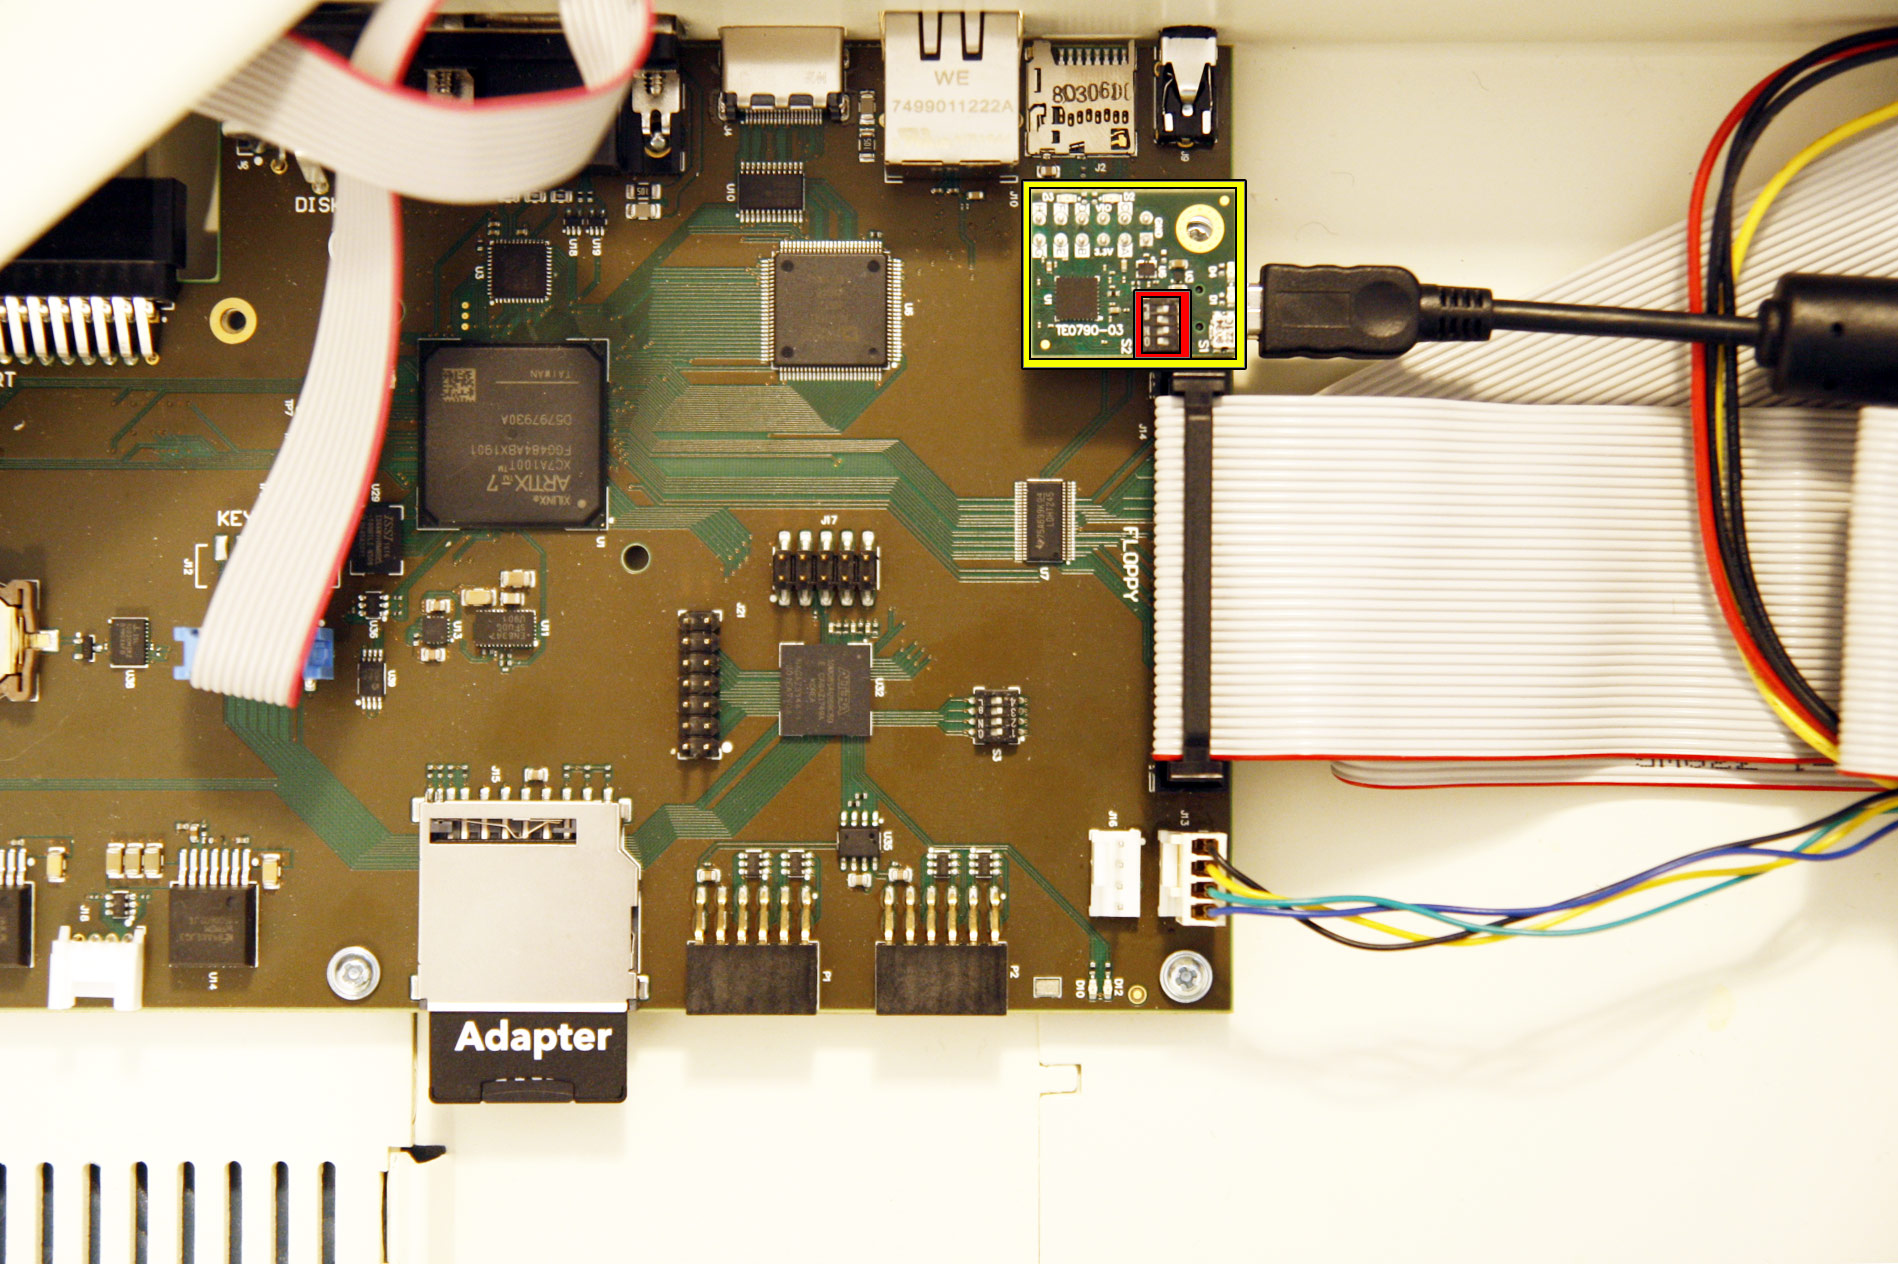
\includegraphics[width=\linewidth]{images/jtag_detail_02.jpg}
\end{tcolorbox}

\begin{tcolorbox}[colback=white,coltext=black]
\underline{Voor eigenaren van een Nexys4-bord}: \\
\\
  Sluit uw micro-USB-kabel aan tussen uw Nexys4-bord en uw pc via de poort met het label ``PROG UART'' (J6), zoals getoond: \\
\\
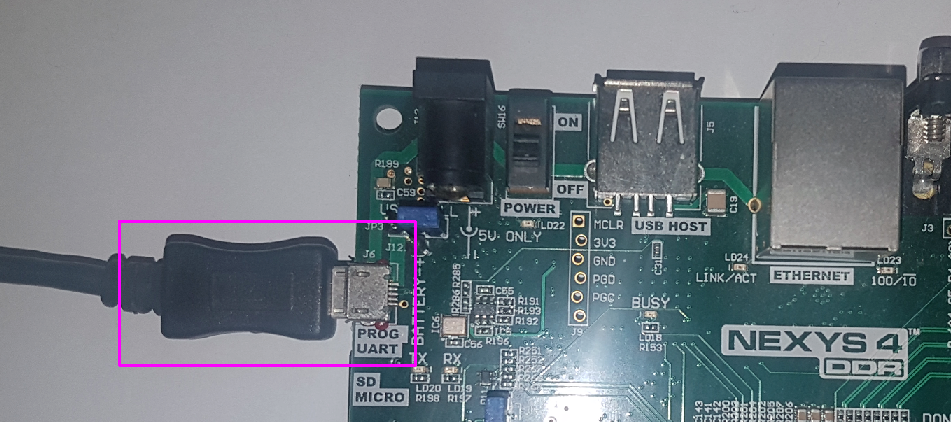
\includegraphics[width=\linewidth]{images/nexys4_comms.png}
\\
\\
Zet bovendien de J1-jumper op de QSPI-stand:
\\
\begin{center}
  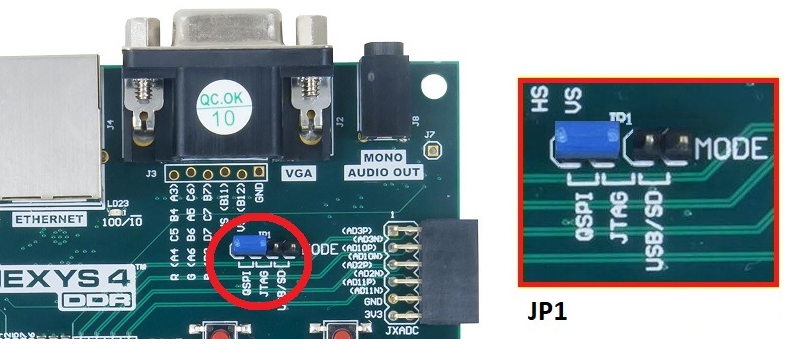
\includegraphics[width=0.8\linewidth]{images/nexys4_j2.png}
\end{center}

\end{tcolorbox}

\begin{itemize}
  \item Sluit uw niet-8-bit computer aan op het FPGA-programmeerapparaat met behulp van de juiste USB-kabel.  \item Schakel de MEGA65-computer in.  \item Open Vivado.
\end{itemize}


\begin{minipage}{\linewidth}
  Stap 1a: Maak een nieuw Vivado-project aan via ``File'', ``Project'', ``New...''. \\  LET OP: Bij toekomstige gelegenheden waarop u de QSPI moet flashen, heropent u dit project (het is niet nodig elke keer een nieuw project aan te maken).  \\
  \begin{center}
    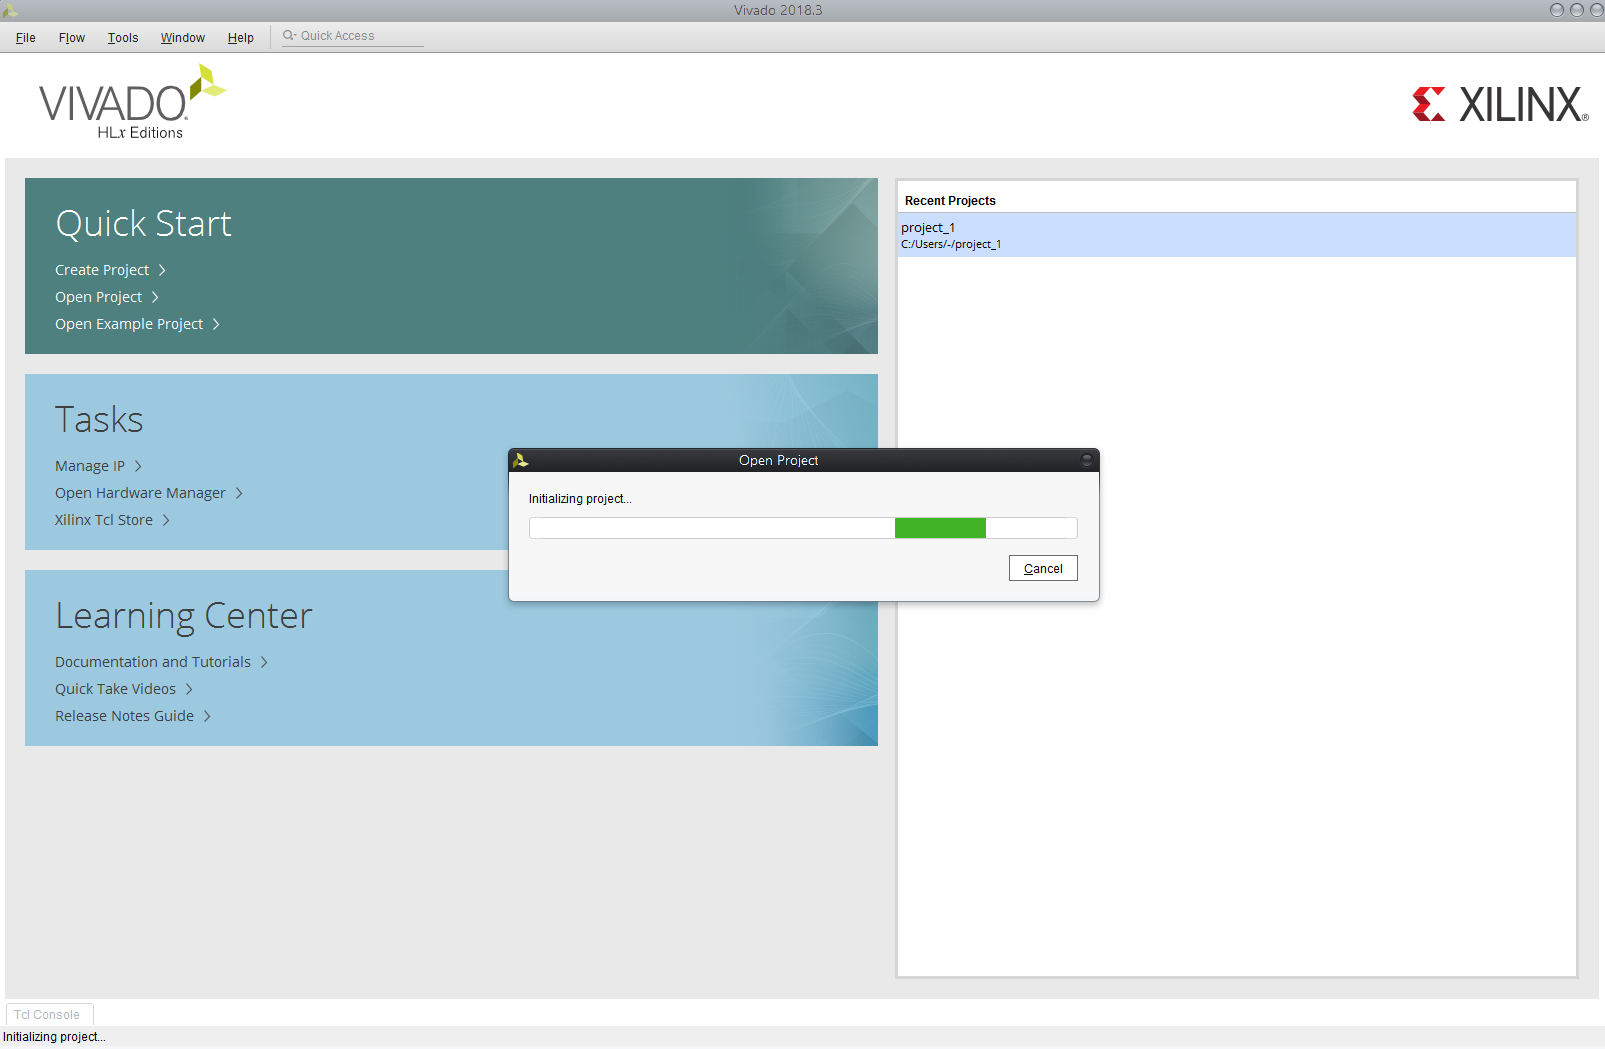
\includegraphics[width=0.8\linewidth]{images/vivado01.png}
  \end{center}
\end{minipage}

\vspace{5mm}

\begin{minipage}{\linewidth}
  Stap 1b: De wizard ``New Project'' verschijnt. Klik op ``Next'': \\
  \begin{center}
    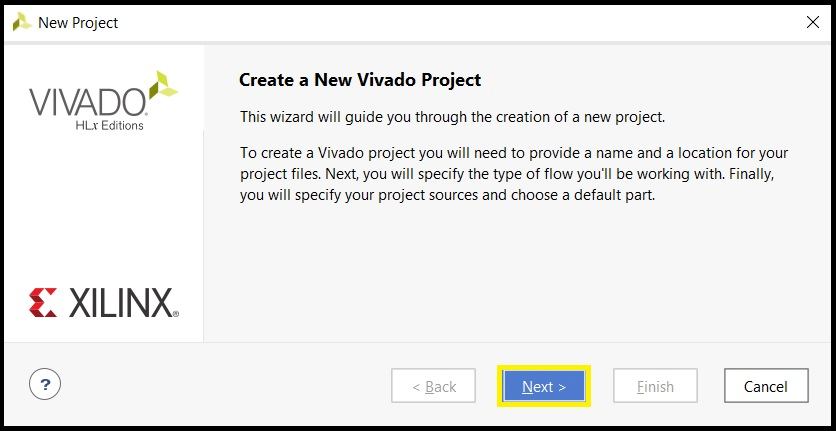
\includegraphics[width=0.8\linewidth]{images/vivado01b.png}
  \end{center}
\end{minipage}

\begin{minipage}{\linewidth}
  Stap 1c: Geef uw project een naam en kies de gewenste locatie en klik op ``Next'':\\
  \begin{center}
    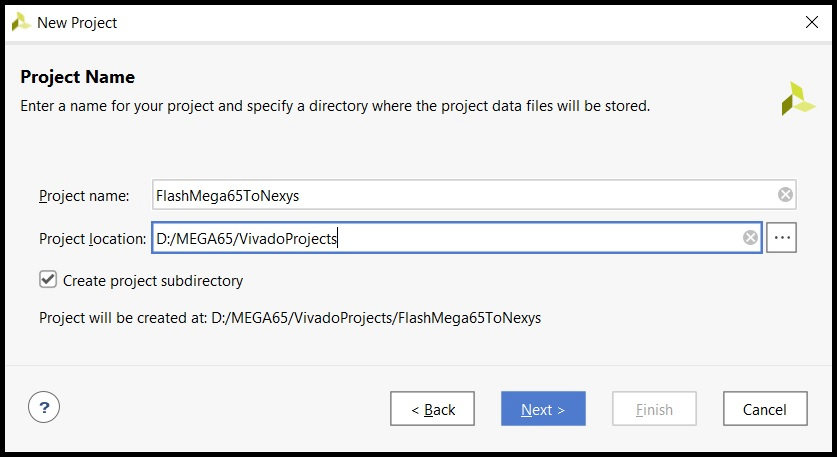
\includegraphics[width=0.8\linewidth]{images/vivado01c.png}
  \end{center}
\end{minipage}

\vspace{5mm}

\begin{minipage}{\linewidth}
  Stap 1d: Laat de standaard geselecteerde opties behouden en klik op ``Next'': \\
  \begin{center}
    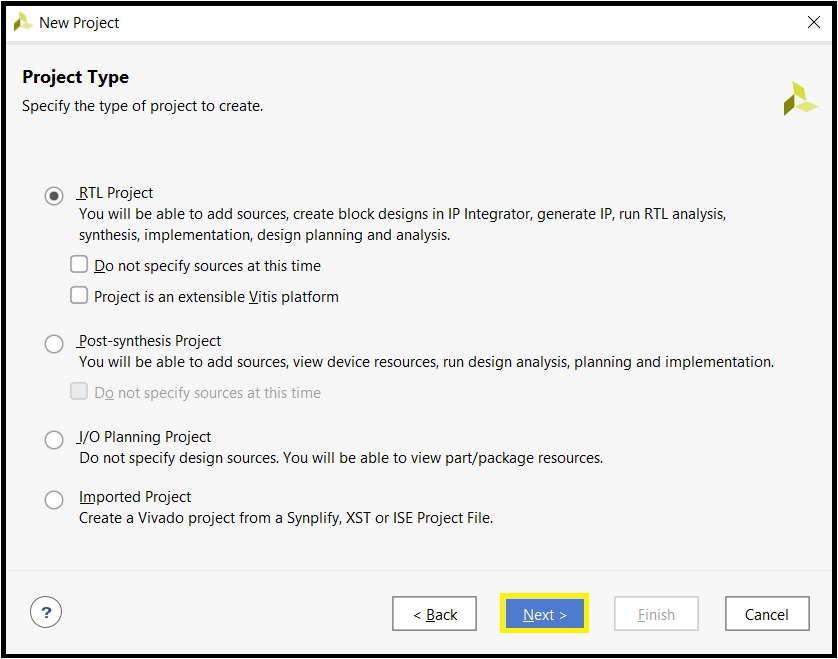
\includegraphics[width=0.8\linewidth]{images/vivado01d.png}
  \end{center}
\end{minipage}

\begin{minipage}{\linewidth}
  Stap 1e: Voeg geen bronnen toe, laat de standaard geselecteerde opties behouden en klik op ``Next'': \\
  \begin{center}
    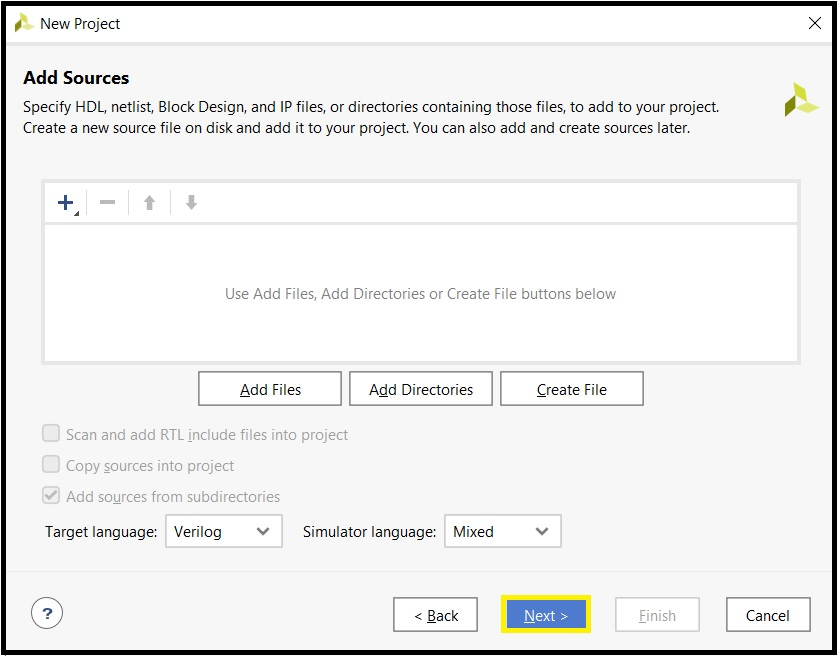
\includegraphics[width=0.7\linewidth]{images/vivado01e.png}
  \end{center}
\end{minipage}

\vspace{5mm}

\begin{minipage}{\linewidth}
  Stap 1f: Laat de standaard geselecteerde opties behouden en klik op ``Next'': \\
  \begin{center}
    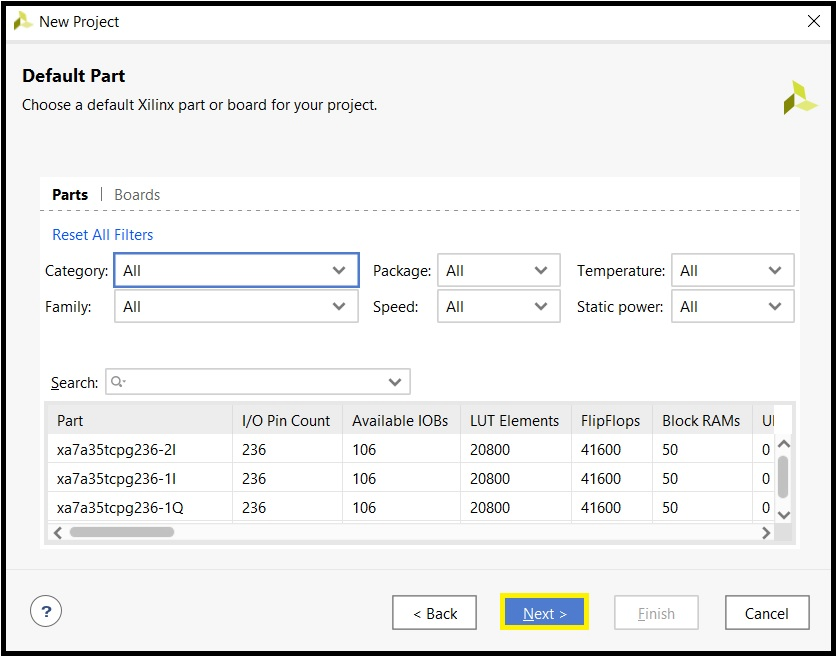
\includegraphics[width=0.7\linewidth]{images/vivado01f.png}
  \end{center}
\end{minipage}

\begin{minipage}{\linewidth}
  Stap 1g: Klik op ``Finish'': \\
  \begin{center}
    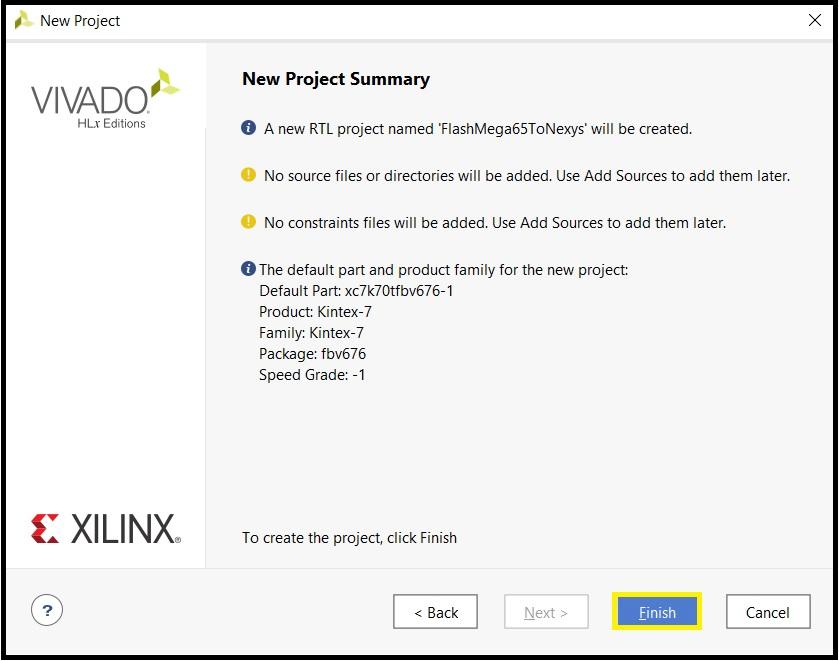
\includegraphics[width=0.8\linewidth]{images/vivado01g.png}
  \end{center}
\end{minipage}

\vspace{5mm}

\begin{minipage}{\linewidth}
  Stap 2: Selecteer in de linker kolom ``Open Hardware Manager'' helemaal onderaan.
  \\
  \begin{center}
    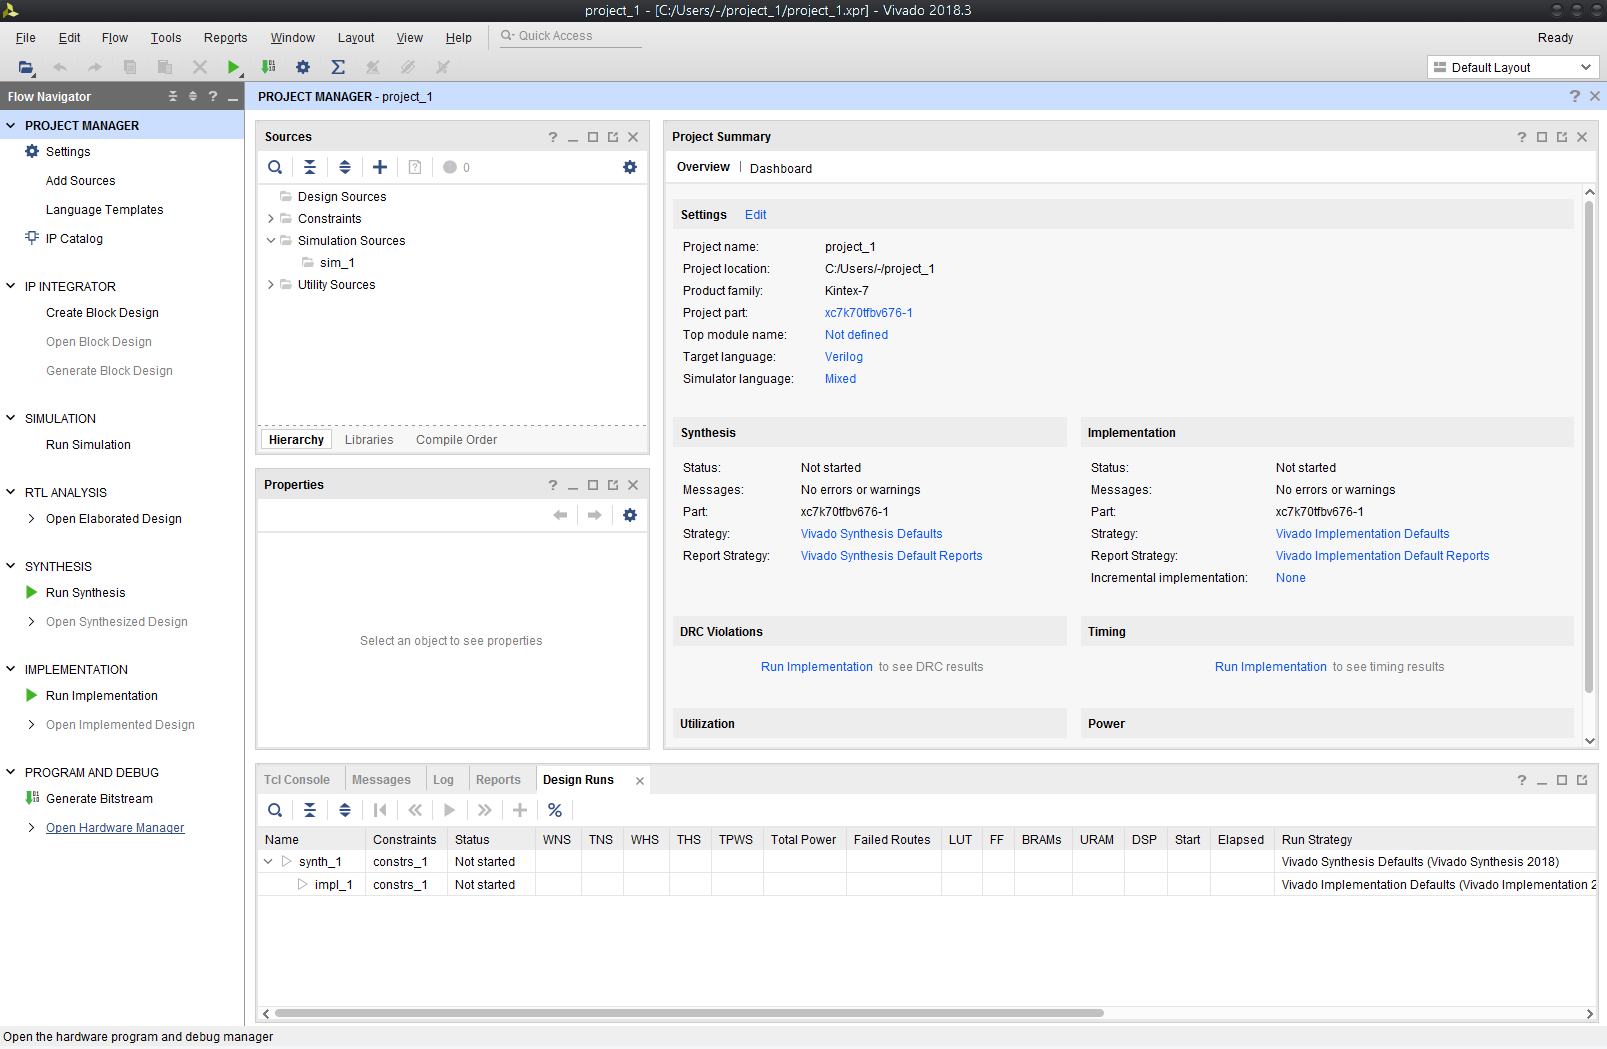
\includegraphics[width=0.8\linewidth]{images/vivado02.png}
  \end{center}
\end{minipage}


\begin{minipage}{\linewidth}
  Stap 3: Verbind met de FPGA: \\  Onder ``Open Hardware Manager'' kiest u ``Open Target'' en vervolgens ``Auto Connect''.
  \\
  \begin{center}
    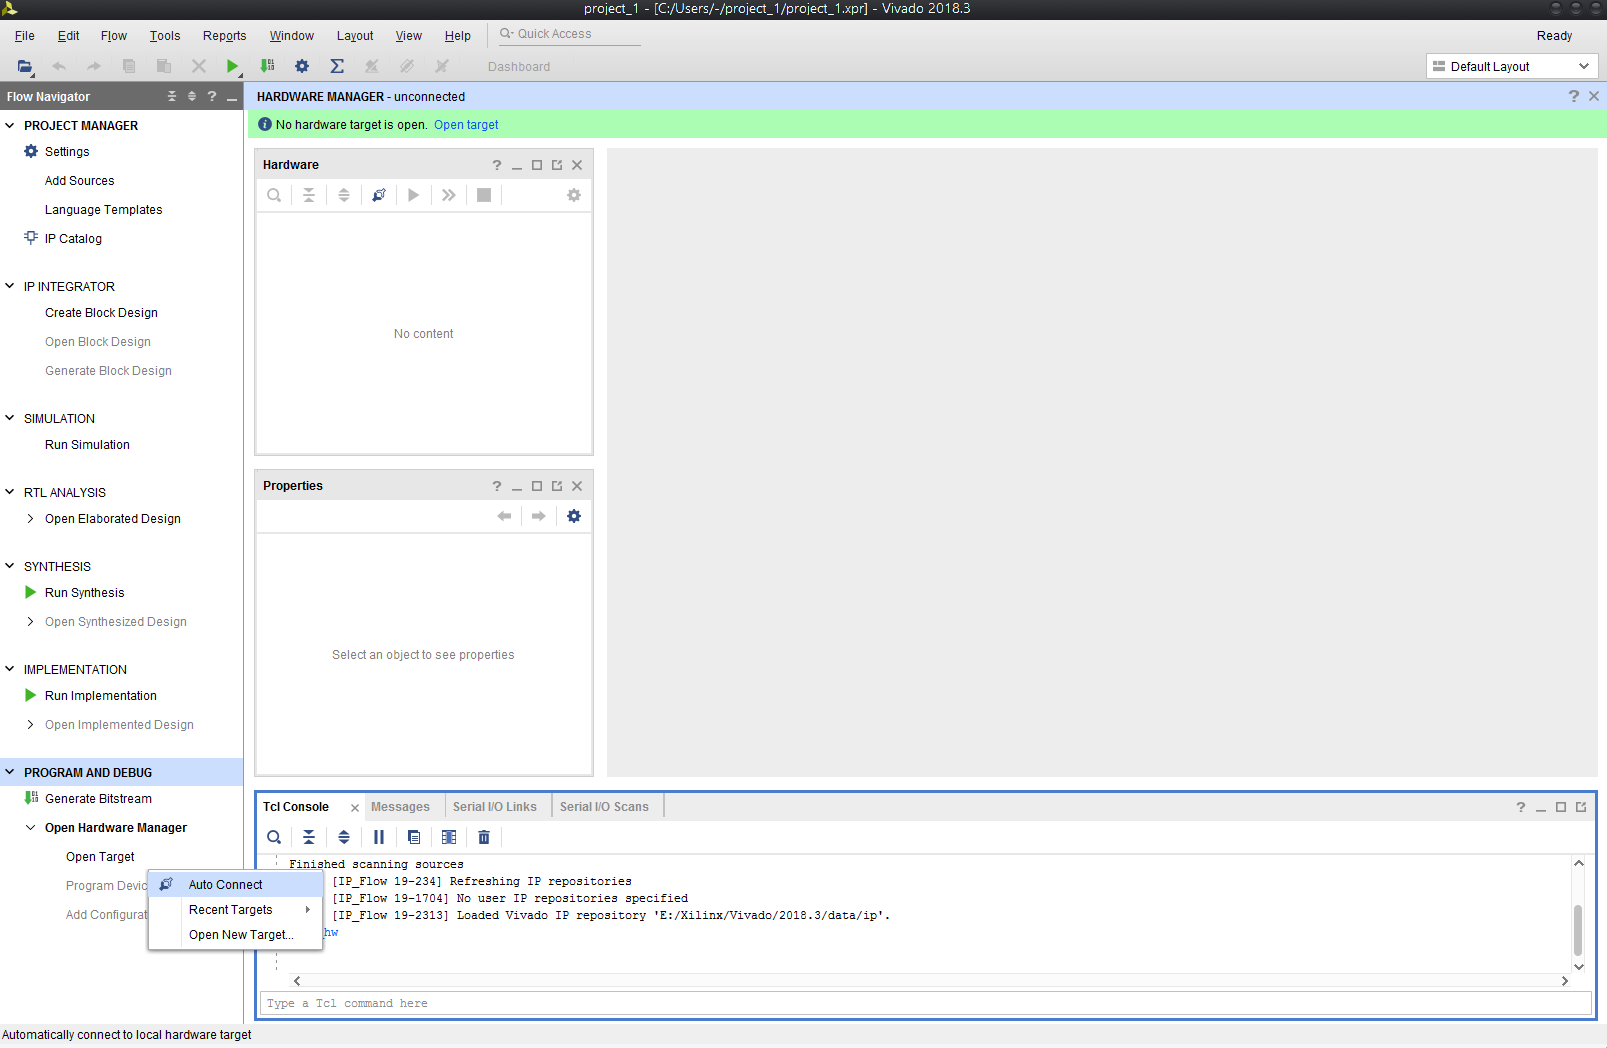
\includegraphics[width=0.8\linewidth]{images/vivado03.png}
  \end{center}
\end{minipage}

\vspace{5mm}

\begin{minipage}{\linewidth}
  Stap 4: Wacht even; ``Connecting to server...'' zou automatisch moeten sluiten zonder een foutmelding aan de console te geven.
  \\
  \begin{center}
    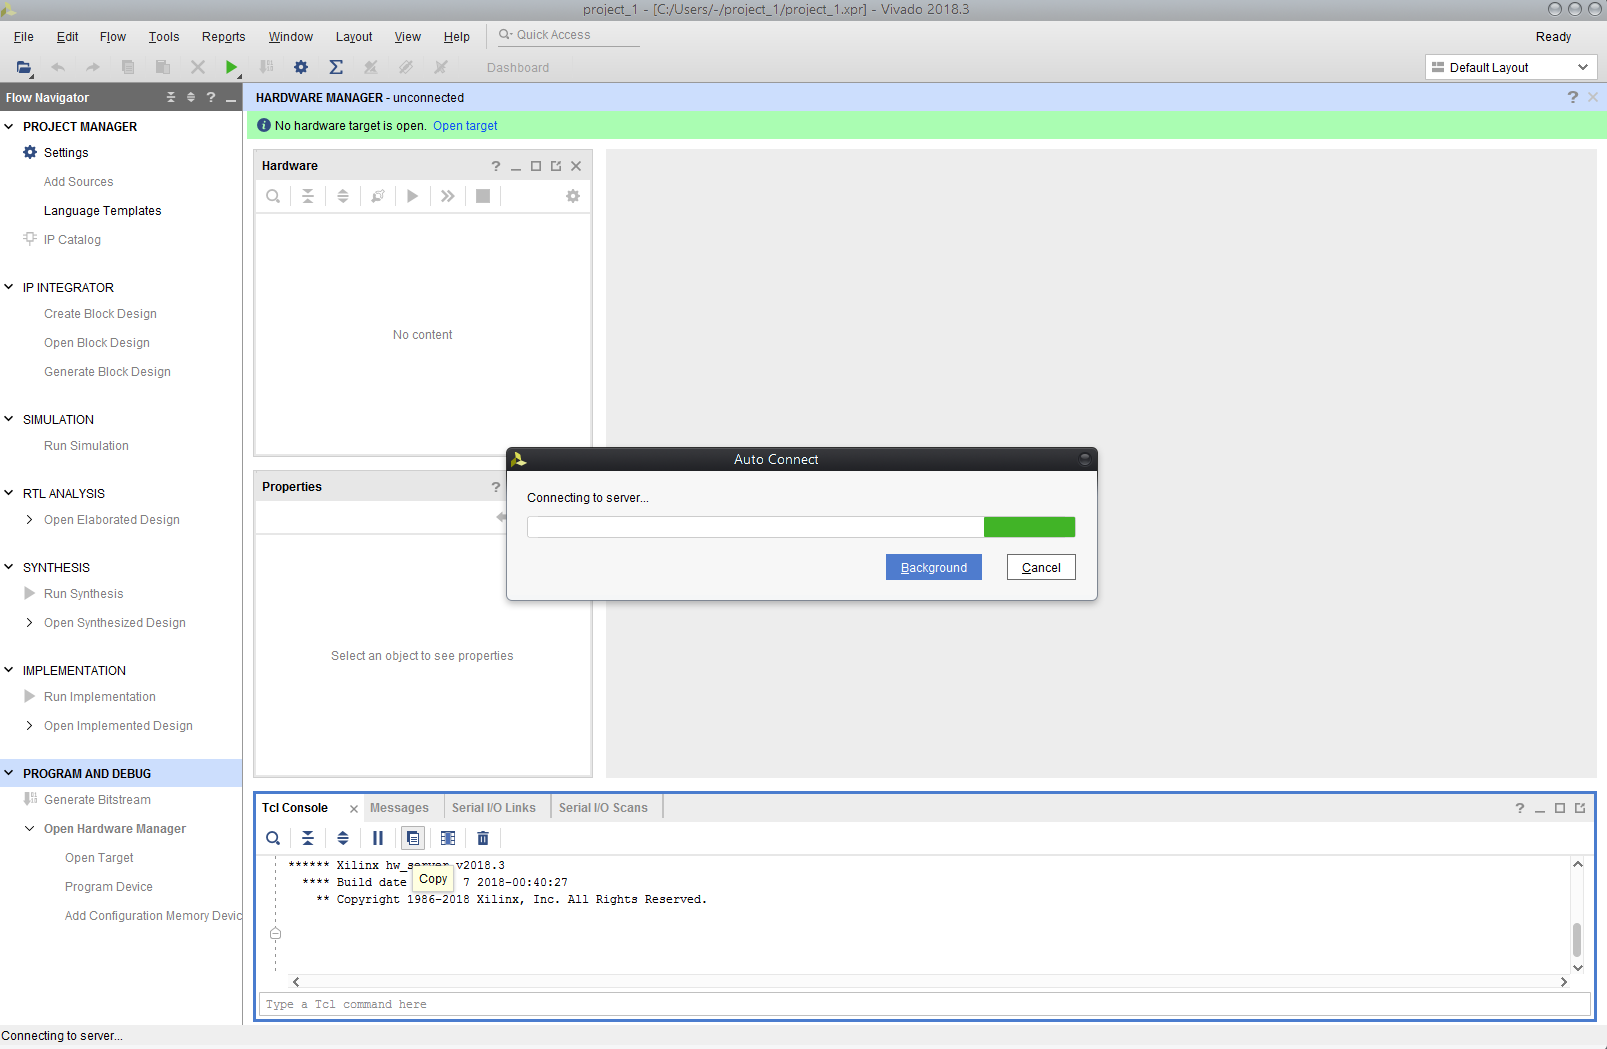
\includegraphics[width=0.8\linewidth]{images/vivado04.png}
  \end{center}
\end{minipage}


\begin{minipage}{\linewidth}
  Stap 5: Onder ``Open Hardware Manager'' kiest u ``Add Configuration Memory Device'' en vervolgens:
  \begin{itemize}
    \item \underline{Voor MEGA65R3/R3A/R4}: ``xc7a200t\_0''    \item \underline{Voor Nexys4 en MEGA65R2}: ``xc7a100t\_0''.
  \end{itemize}

  \begin{center}
    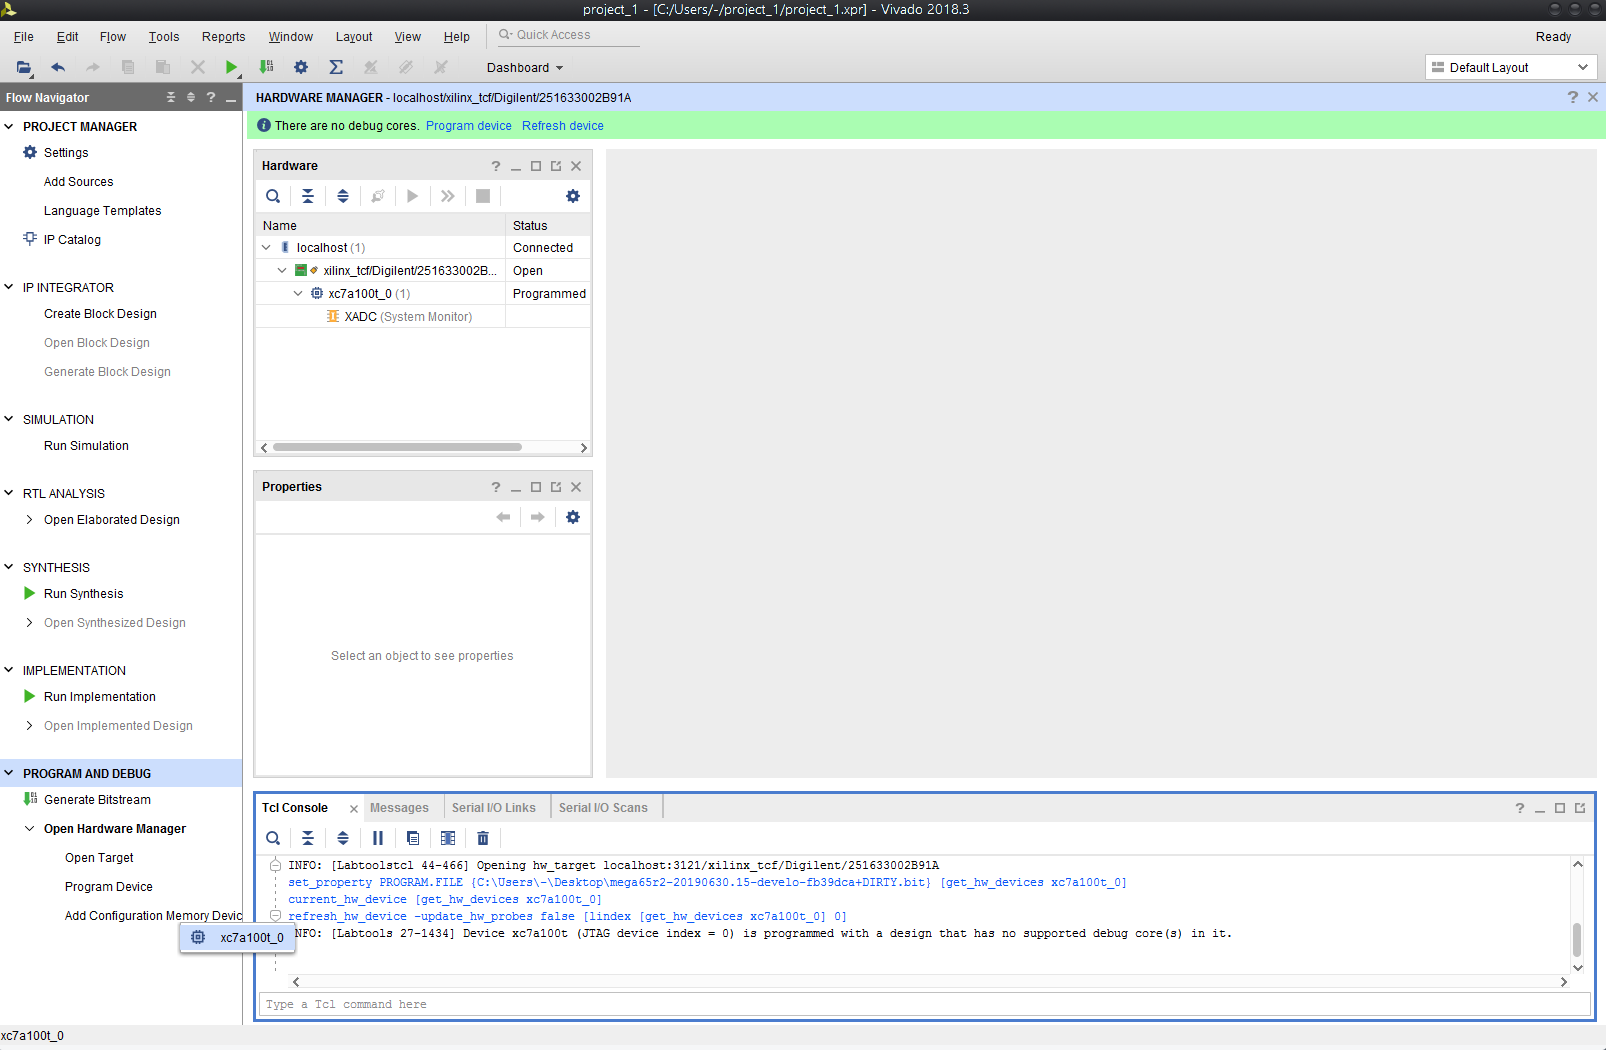
\includegraphics[width=0.7\linewidth]{images/vivado05.png}
  \end{center}
\end{minipage}

\vspace{5mm}

\begin{minipage}{\linewidth}
  Stap 6a: Selecteer Memory Part: \\
  \\
  In het nieuw geopende dialoogvenster:
  \begin{itemize}
    \item \underline{Voor MEGA65R2/R3}: typ ``S25fl256s''    (zonder aanhalingstekens), selecteer vervolgens ``s25fl256sxxxxxxx0-spi-x1\_x2\_x4''    (de bovenste) en klik op ``OK''.    \item \underline{Voor MEGA65R3A/R4}: Vivado kan het grotere flashgeheugen op deze borden niet flashen. Gebruik het flashmenu op de MEGA65.    \item \underline{Voor Nexys4}: typ ``S25fl128s''    (zonder aanhalingstekens), selecteer vervolgens ``s25fl128sxxxxxxx0-spi-x1\_x2\_x4''    (de bovenste) en klik op ``OK''.
  \end{itemize}

  \begin{center}
    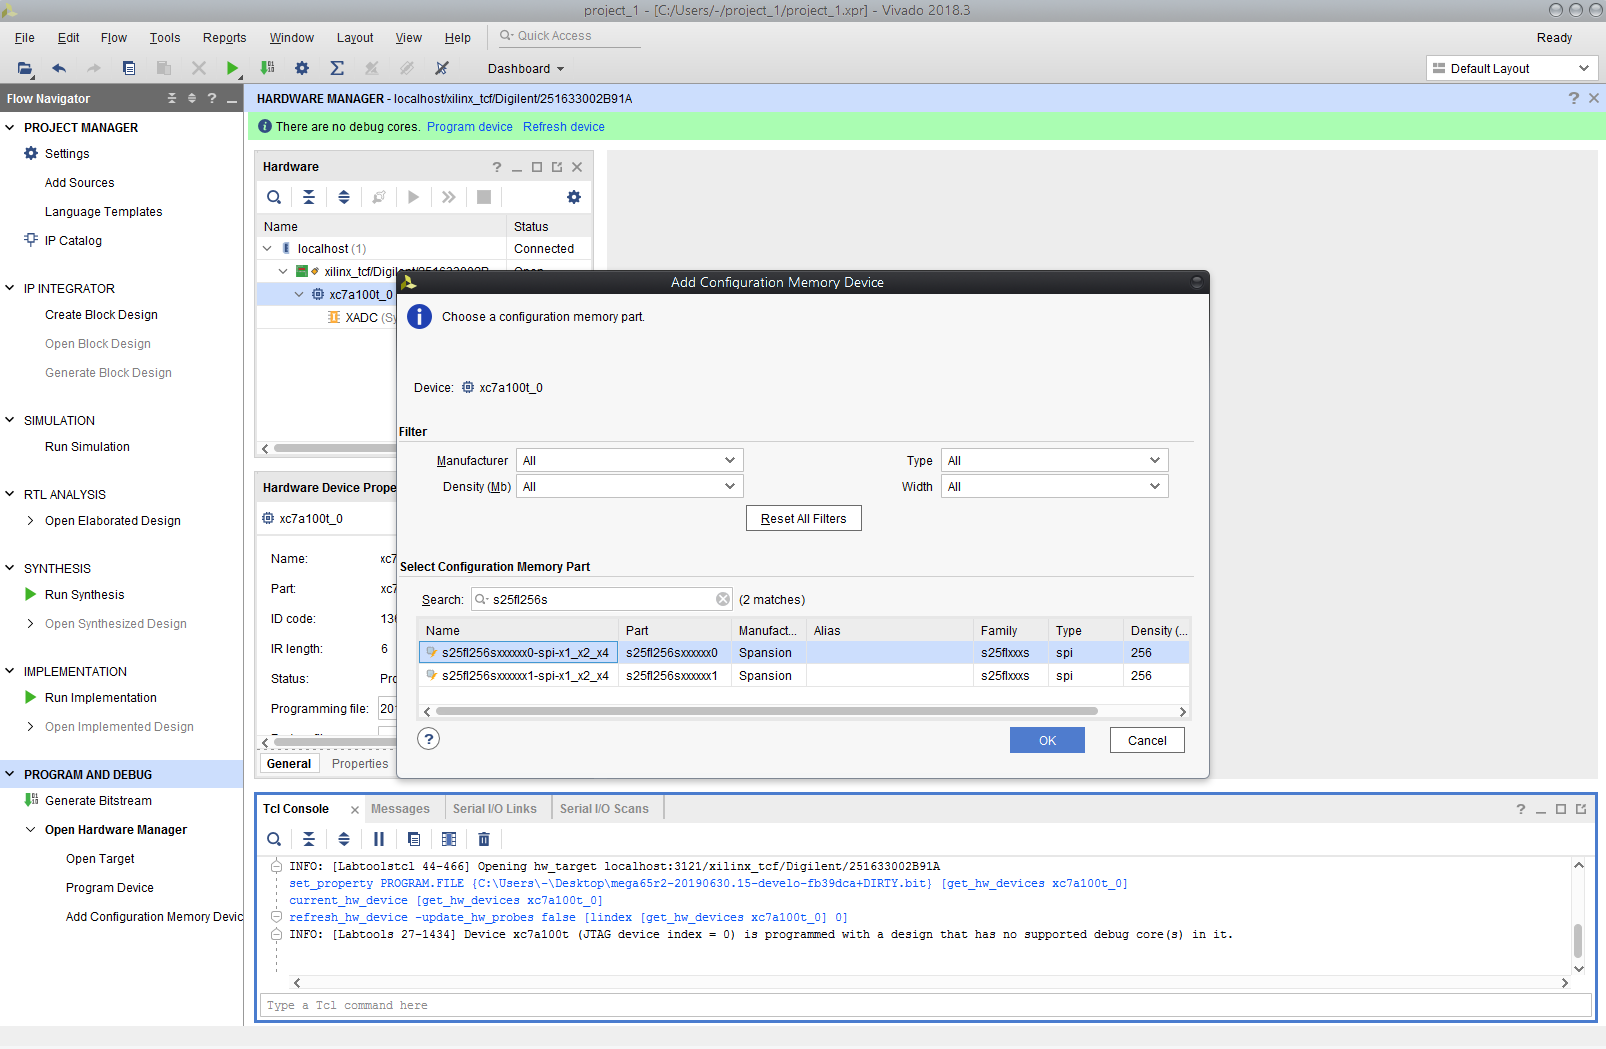
\includegraphics[width=0.7\linewidth]{images/vivado06.png}
  \end{center}
\end{minipage}

\begin{minipage}{\linewidth}
  Stap 6b: Klik op ``OK'' om te bevestigen dat u het configuratiegeheugenapparaat nu wilt programmeren.
  \begin{center}
    \includegraphics[width=0.85\linewidth]{images/vivado06b.png}
  \end{center}
\end{minipage}

\begin{minipage}{\linewidth}
  Stap 6c: Als u zo'n pop-up niet ziet of de QSPI op een later tijdstip opnieuw wilt programmeren, klikt u in het ``Hardware''-venster met de rechtermuisknop op de geheugenconfiguratie en selecteert u ``Program Configuration Memory Device'':
  \begin{center}
    \includegraphics[width=0.85\linewidth]{images/vivado06c.png}
  \end{center}
\end{minipage}

\begin{minipage}{\linewidth}
  Stap 7: Stel de programmeeropties in: \\  Stel in het volgende dialoogvenster ``Configuration file'' in op het pad van uw ``.mcs''-bitstream-bestand. U kunt optioneel ook het ``PRM file''-veld instellen op het pad van uw ``.prm''-bestand. Laat alle overige parameters zoals ze zijn (zie onderstaande screenshot).
  \\
  \begin{center}
    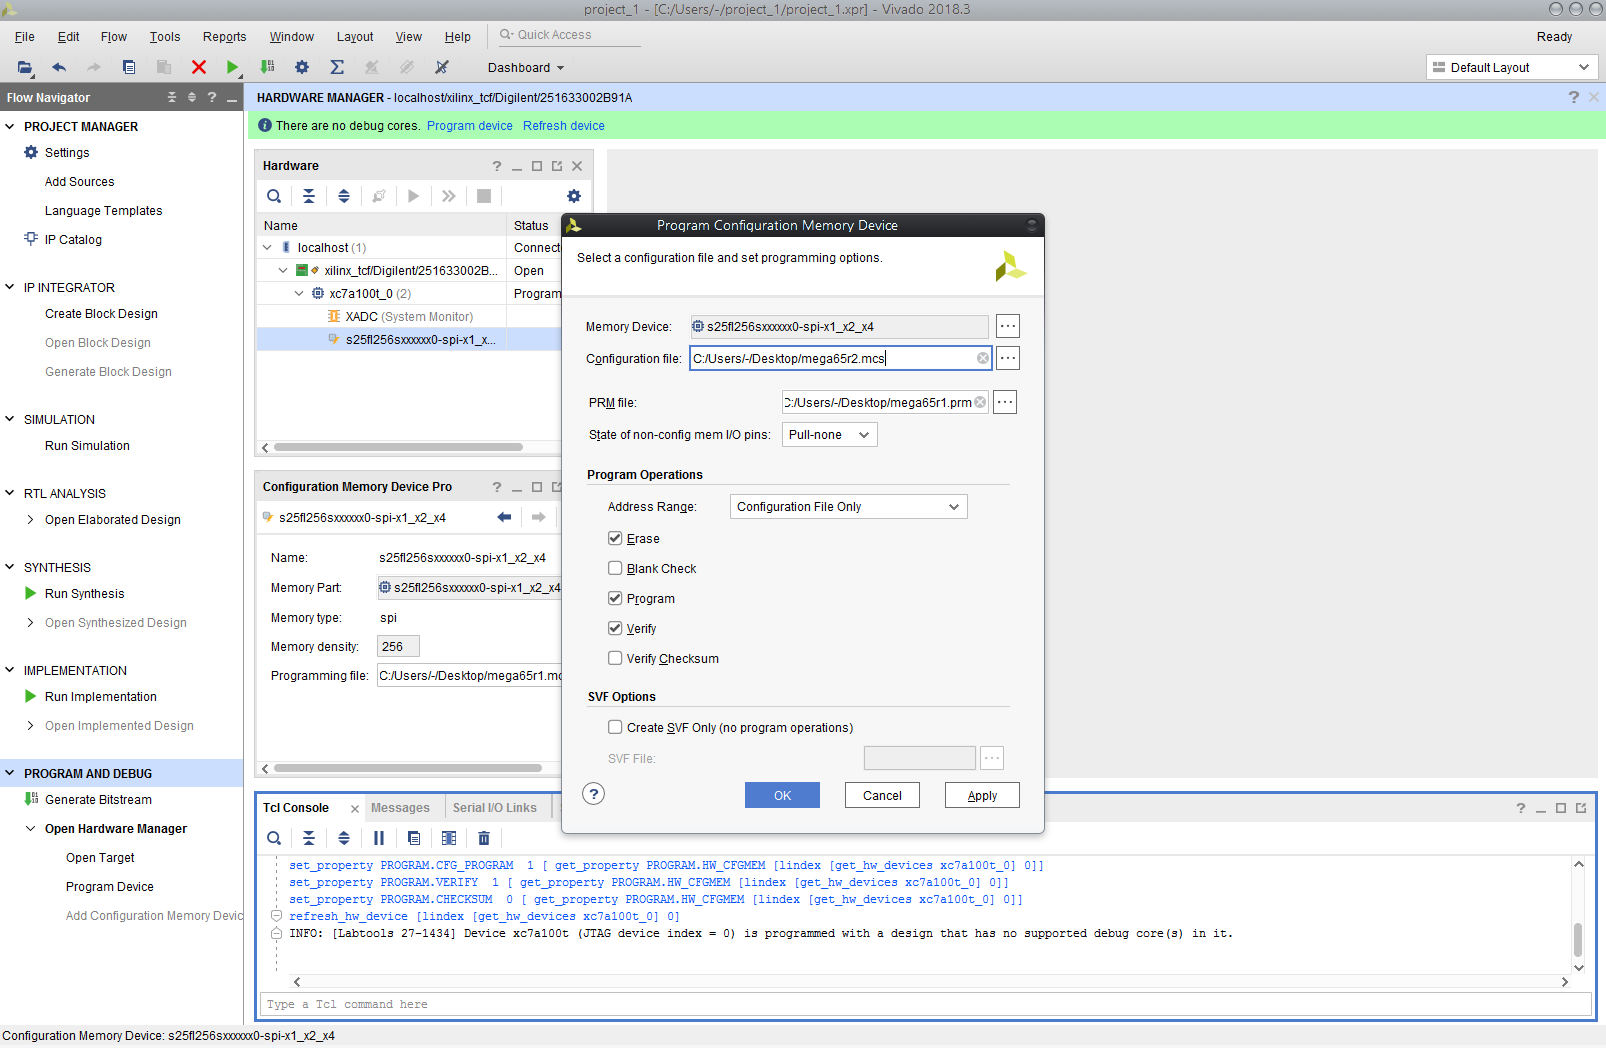
\includegraphics[width=0.85\linewidth]{images/vivado07.png}
  \end{center}
\end{minipage}

\vspace{1mm}

\begin{minipage}{\linewidth}
  Stap 8: Wacht geduldig tot het programmeren is voltooid.  Dit kan enkele minuten duren, omdat de Vivado-software het flashgeheugen dat wordt gebruikt om de FPGA bij het inschakelen te initialiseren, eerst wist en vervolgens opnieuw programmeert.
  \\
  \begin{center}
    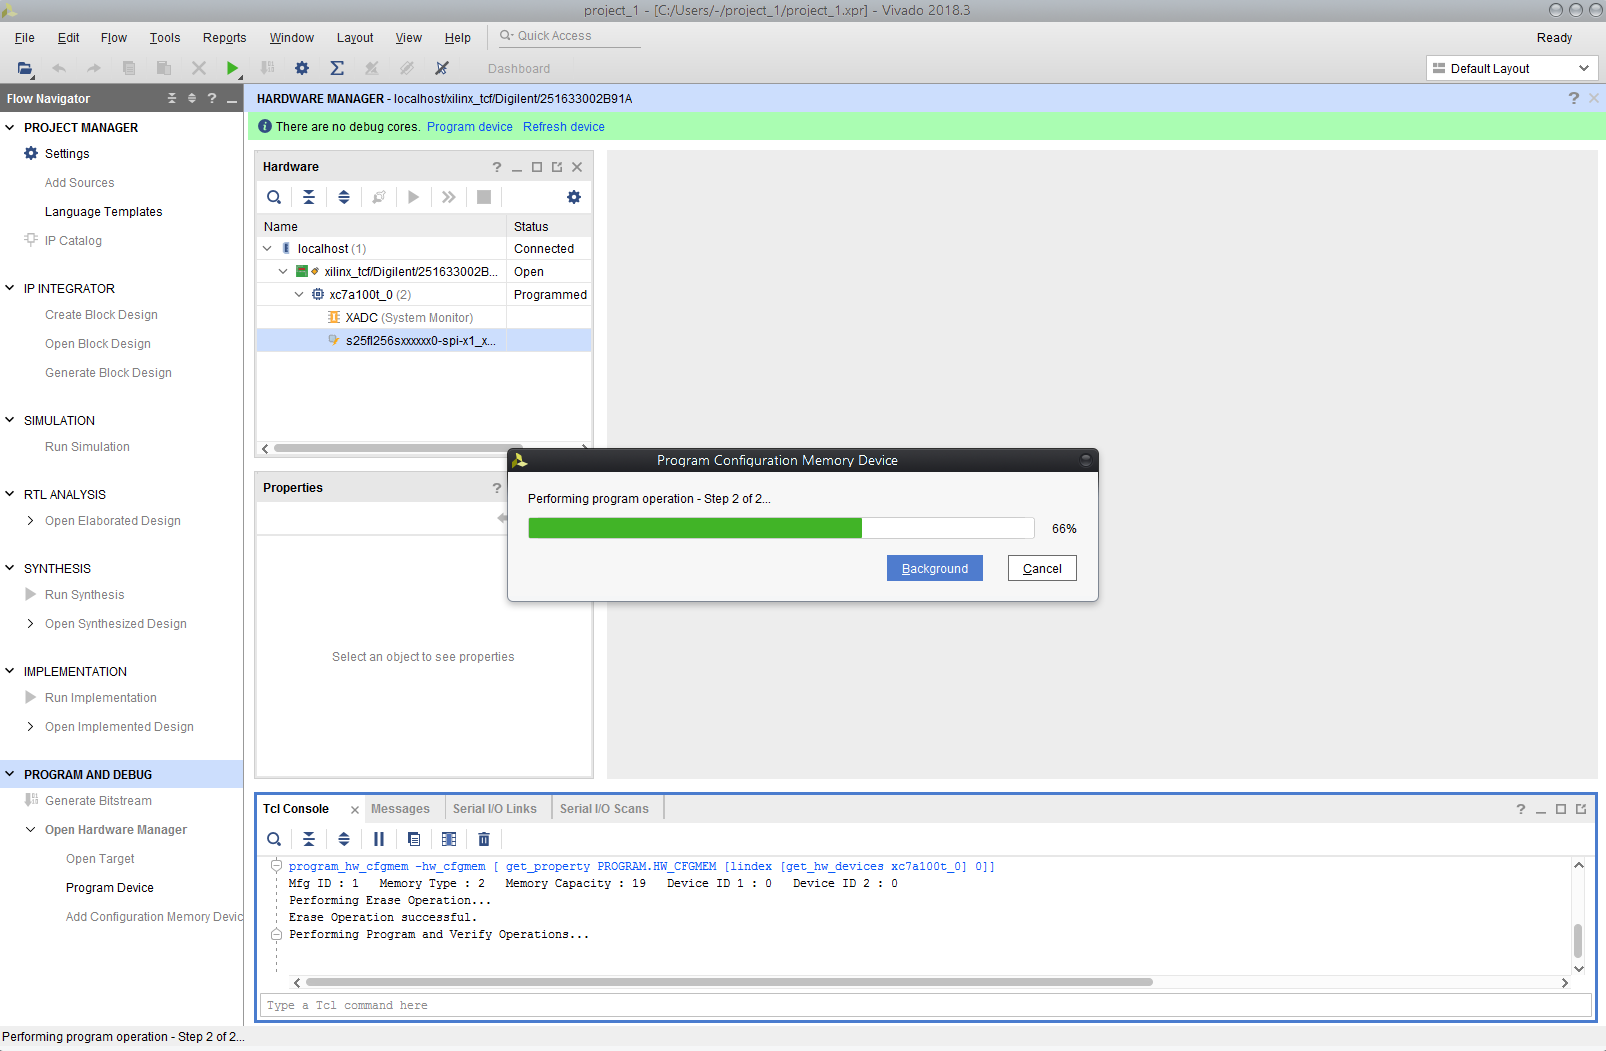
\includegraphics[width=0.85\linewidth]{images/vivado08.png}
  \end{center}
\end{minipage}


\begin{minipage}{\linewidth}
Stap 9: Als uw scherm eruitziet als de onderstaande screenshot, is uw nieuwe bitstream succesvol geflasht in Slot 0 van uw QSPI-flashgeheugen!
  \\
  \begin{center}
    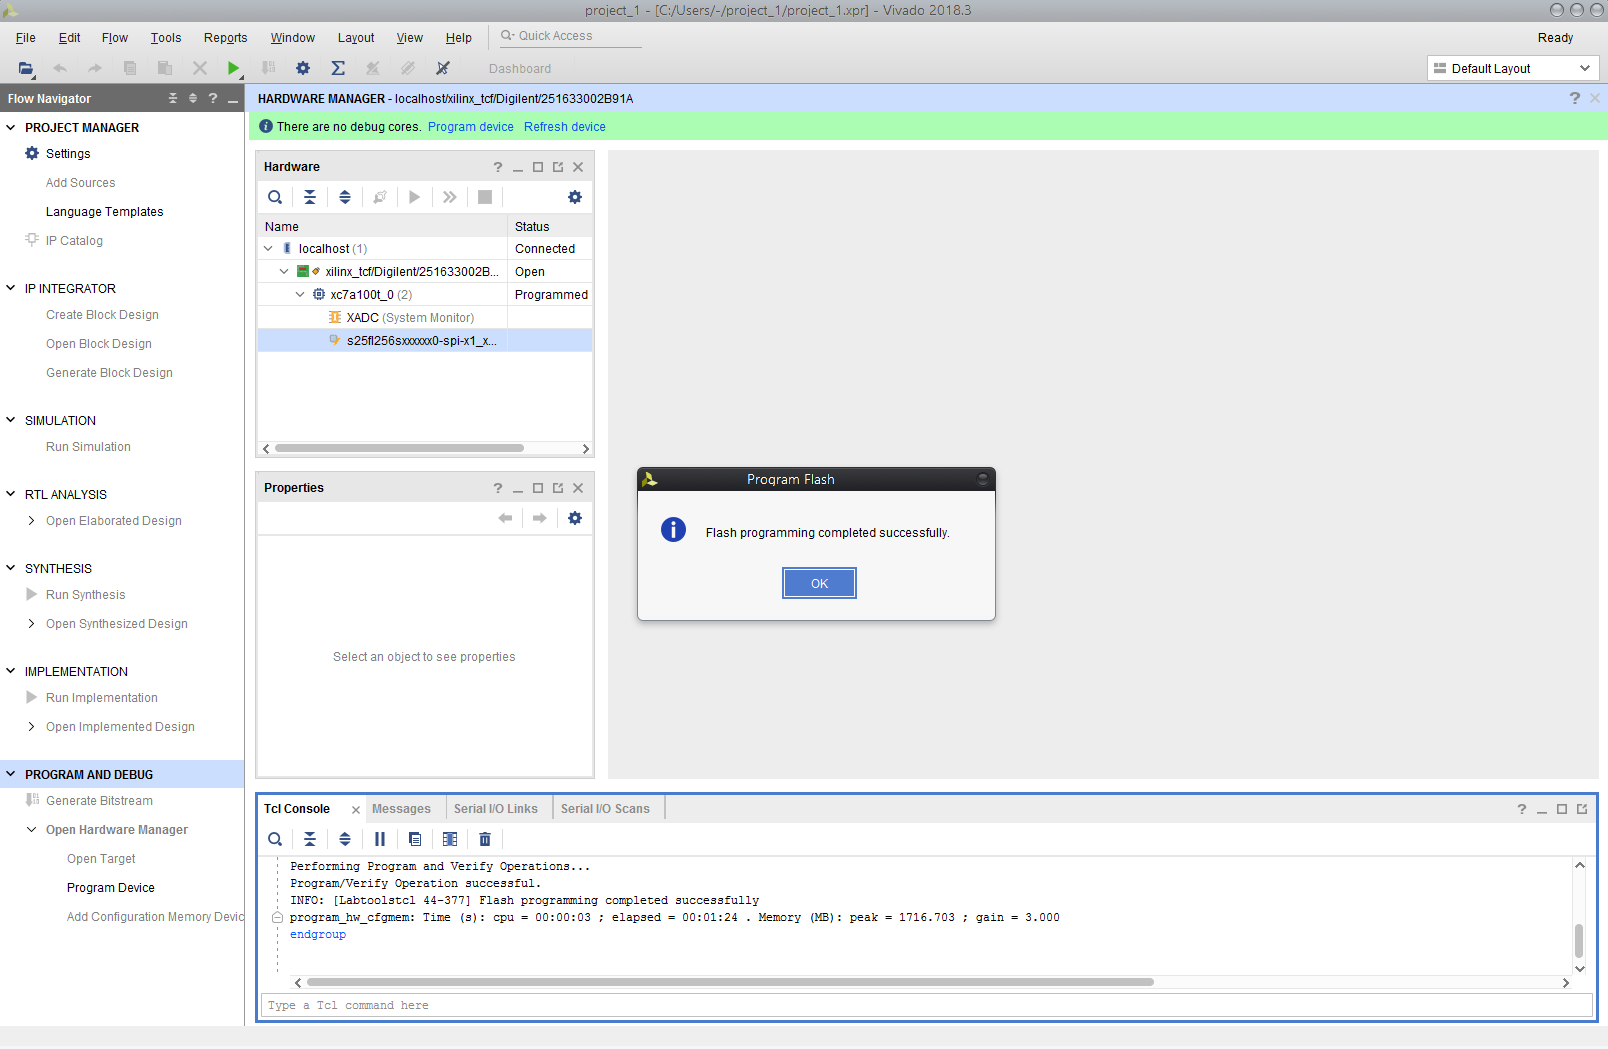
\includegraphics[width=0.8\linewidth]{images/vivado09.png}
  \end{center}
\end{minipage}

\vspace{5mm}

\begin{minipage}{\linewidth}
Stap 10: Als u de FPGA opnieuw wilt flashen, kan het zijn dat de optie ``Add Configuration Memory Device'' uit stap 5 grijs weergegeven wordt.
Selecteer in dat geval ``s25fl256sxxxxxxx0-spi-x1\_x2\_x4''  in het ``Hardware''-venster, druk op de rechtermuisknop en selecteer ``Program Configuration Memory Device'' om te flashen.
  \\
  \begin{center}
    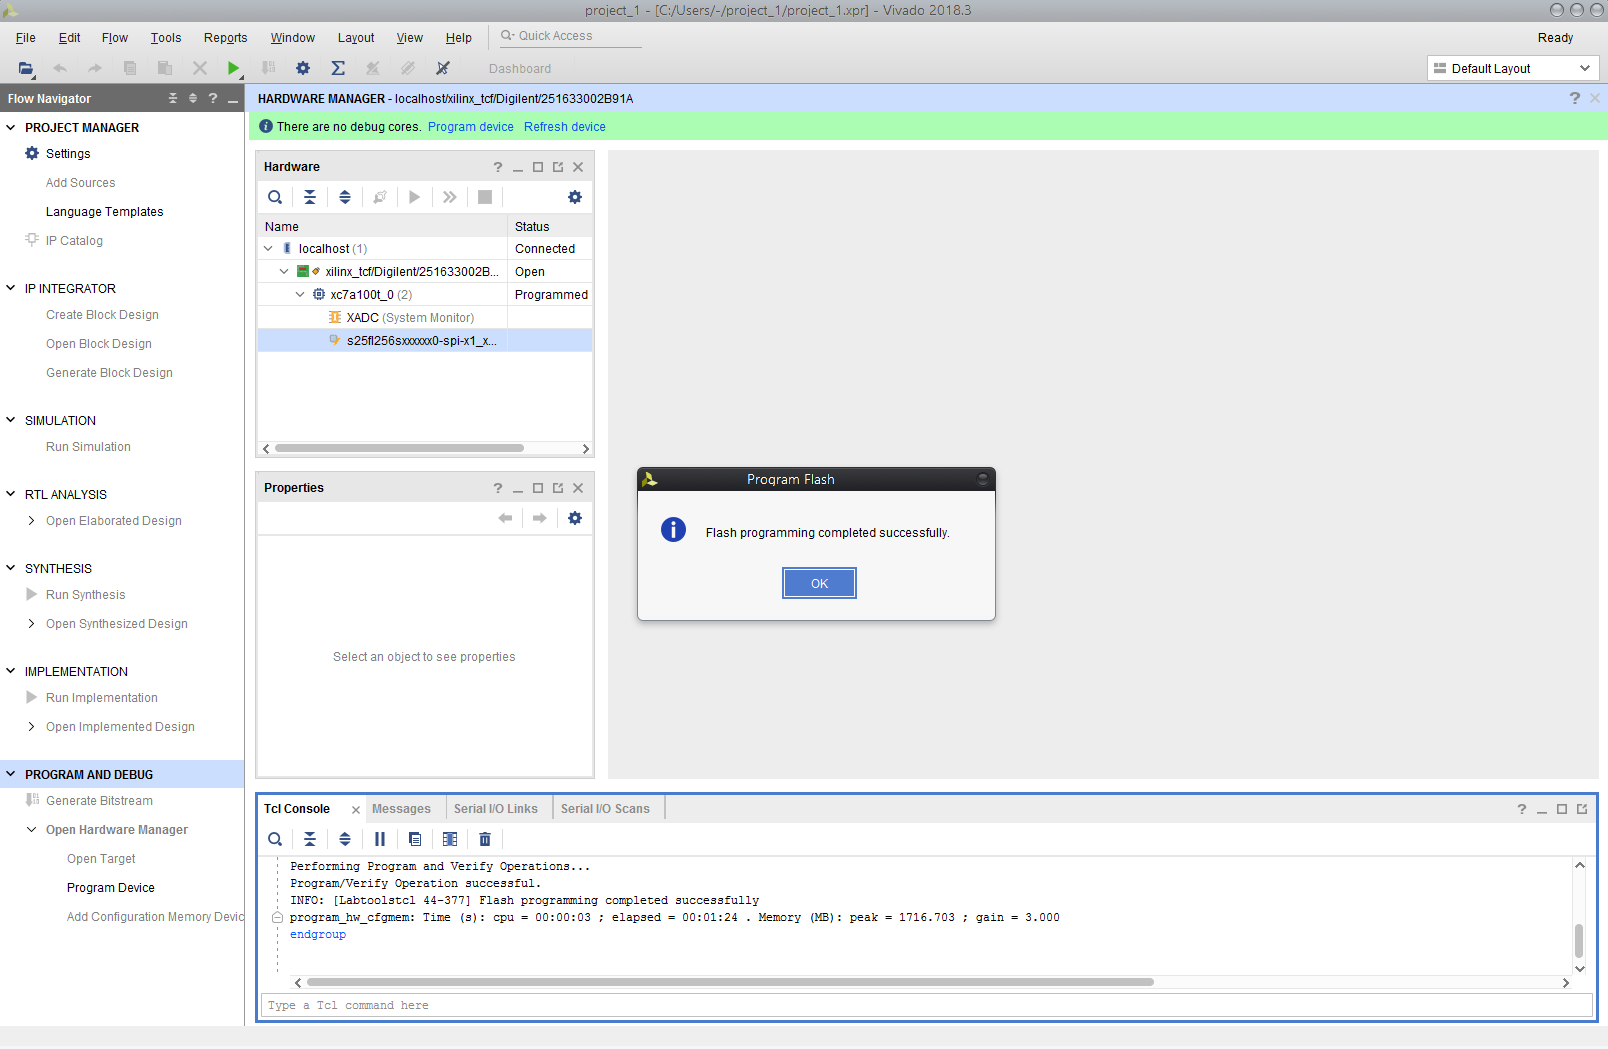
\includegraphics[width=0.8\linewidth]{images/vivado09.png}
  \end{center}
\end{minipage}


\section{De CPLD in het toetsenbord van de MEGA65 flashen met Lattice Diamond}
\label{sec:flashcpld}


Indien u ervoor kiest om door te gaan, heeft u een TE0790-03 JTAG-programmeermodule en een werkende installatie van Lattice Diamond Programmer-software nodig. Dit kan op zowel Windows als Linux, maar in beide gevallen moet u de benodigde USB-stuurprogramma's installeren. Het is ook noodzakelijk dat dip-schakelaars 1 en 3 op de AAN-stand staan en dip-schakelaars 2 en 4 op de UIT-stand op de TE-0790. Met de MEGA65 losgekoppeld van de voeding moet de TE-0790 op de JB1-connector worden geïnstalleerd, die zich tussen de diskettedatakabel en de audiojack bevindt. De vergulde opening van de TE-0790 moet in lijn liggen met het schroefgat eronder. De mini-USB-kabel verbindt zich vervolgens aan de kant richting het 3.5'' diskettestation. De volgende afbeelding toont de juiste positie: de TE0790 is omringd door de gele kast en de dip-schakelaars door de rode kast. Dip-schakelaar 1 is de dichtstbijzijnde bij de diskettedatakabel.


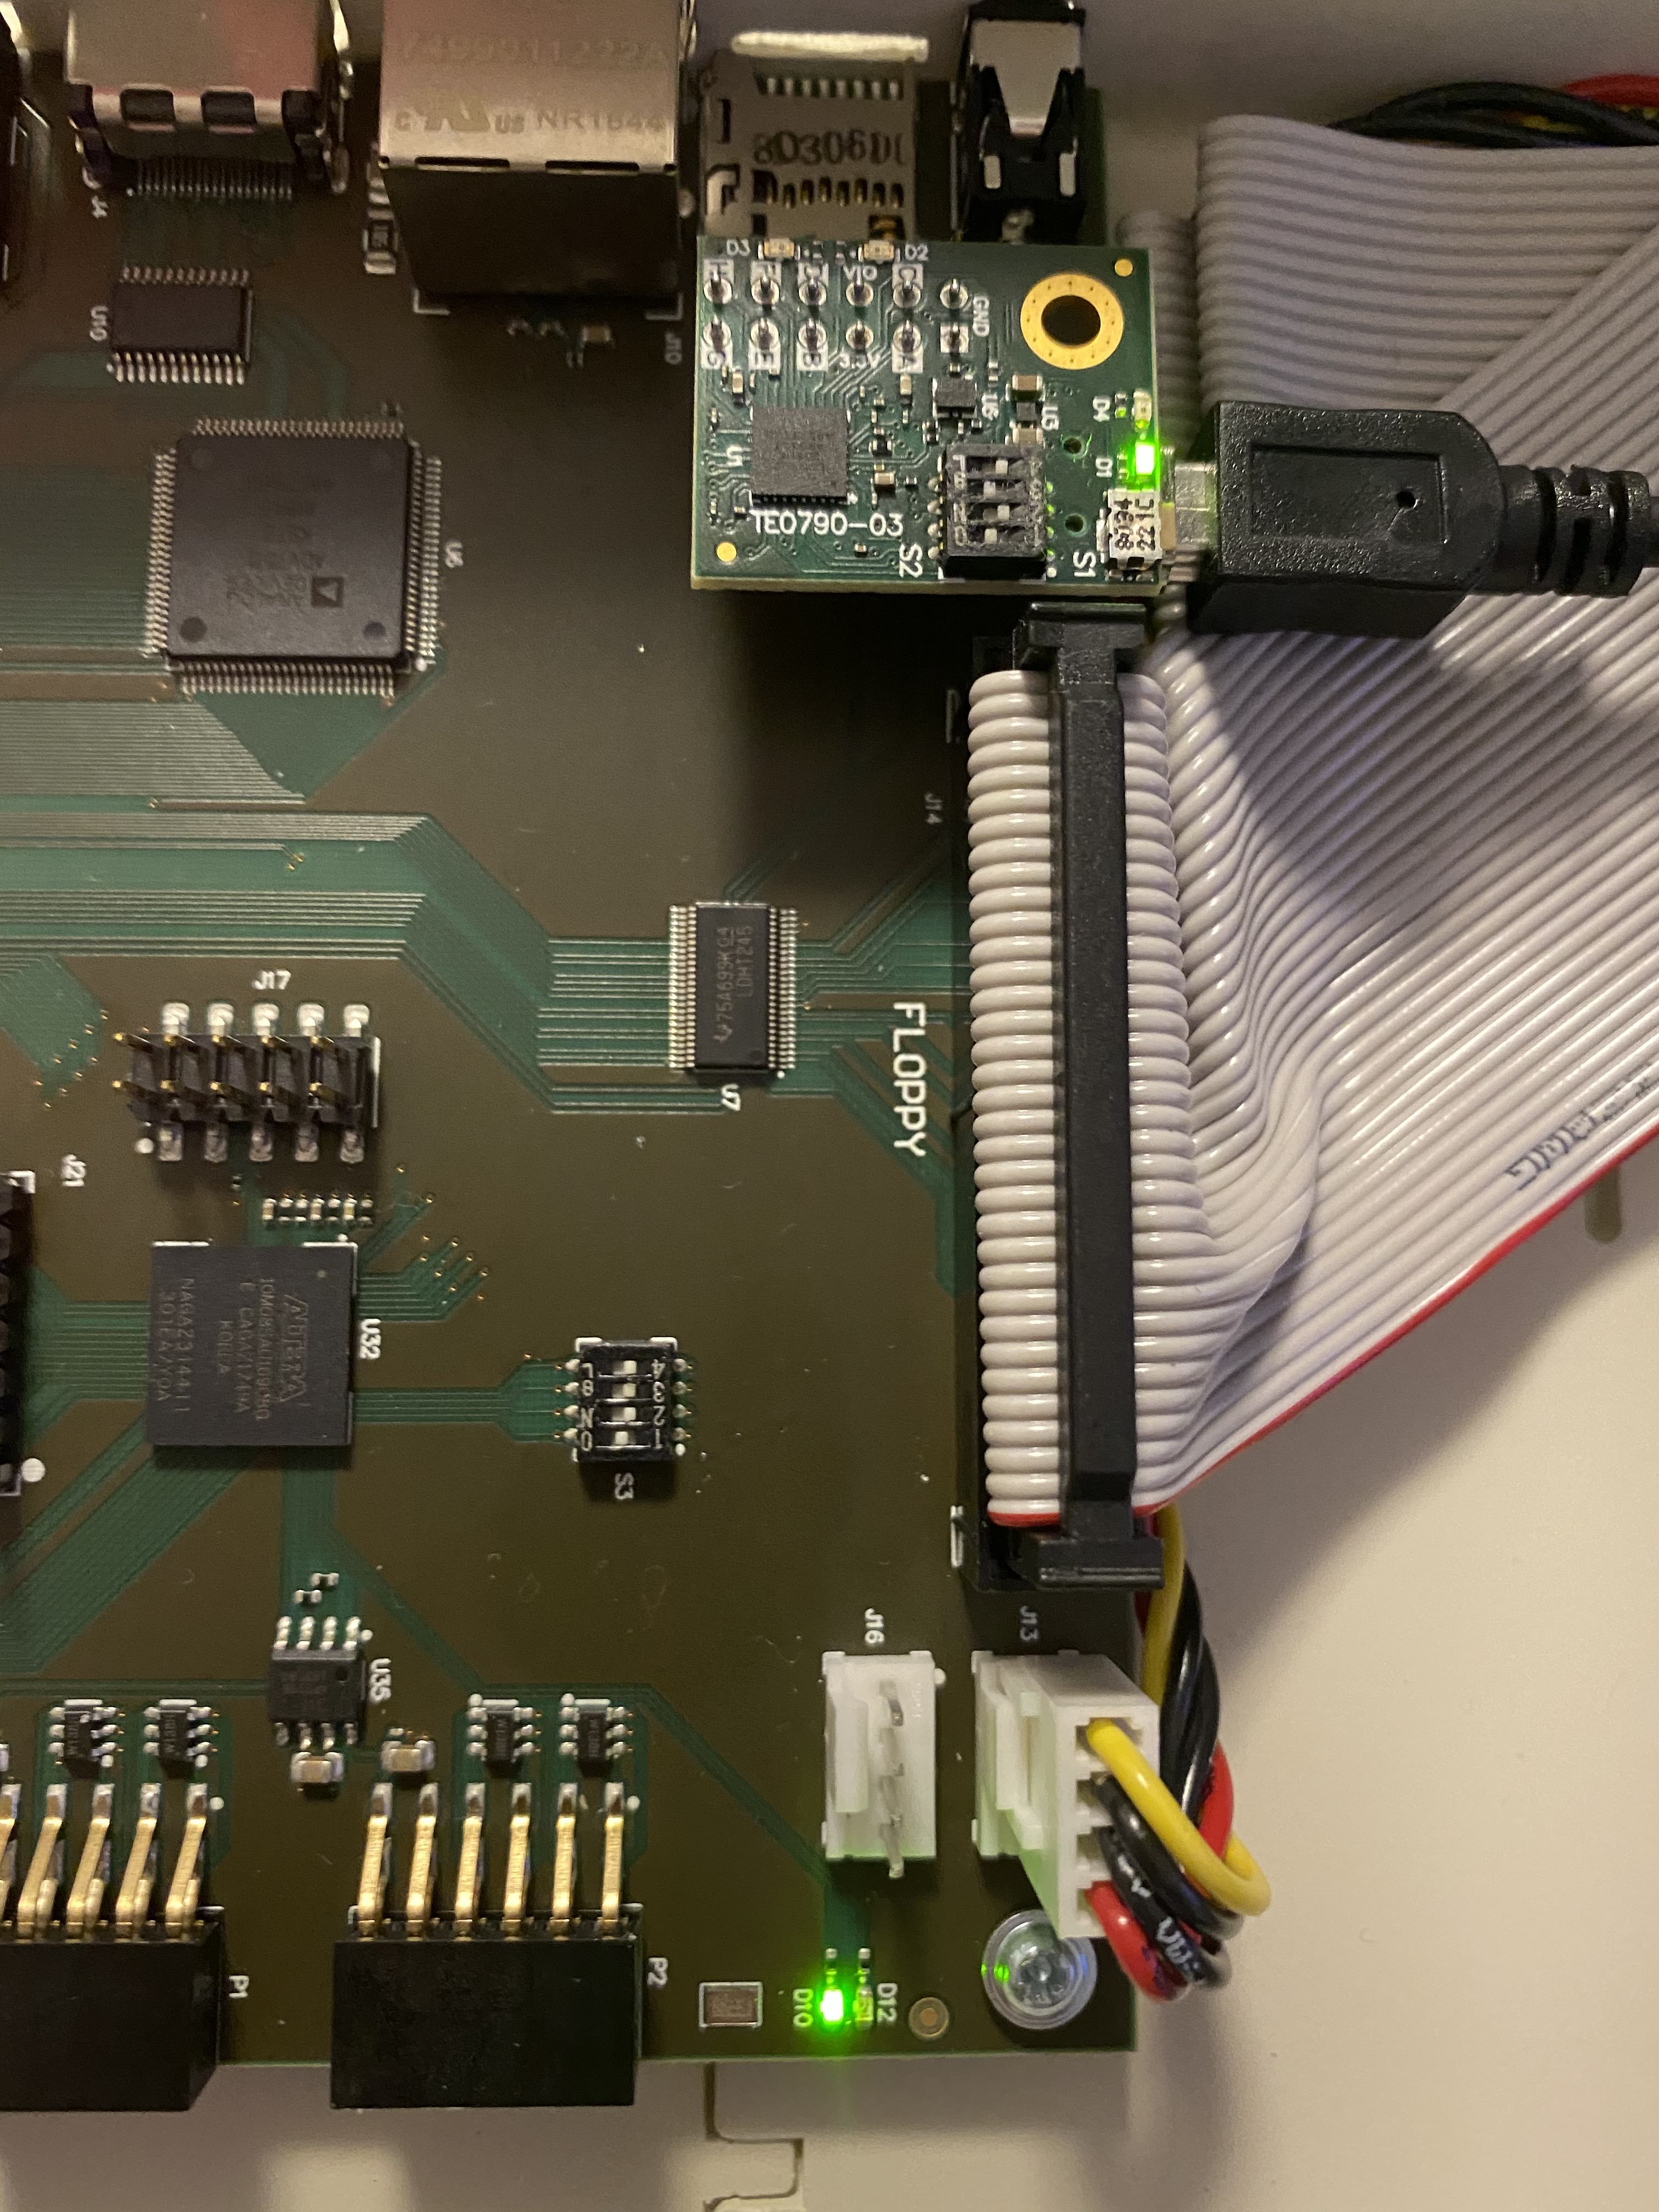
\includegraphics[width=\linewidth]{images/jtag_detail_05.jpg}


Op de PCB van een R2/R3/R3A/R4 MEGA65-moederbord moet dip-schakelaar 1 (de dichtstbijzijnde bij de gebruiker die voor de computer zit) op de AAN-stand staan. De overige schakelaars moeten UIT staan. Het toetsenbord gaat in de ``ambulance-modus'' (blauwe flitsende lichten) wanneer het correct is ingesteld.

Sluit uw niet-8-bit computer aan op het FPGA-programmeerapparaat met behulp van een mini-USB-kabel. Schakel de MEGA65-computer in. Open de Diamond Programmer, die van het internet kan worden gedownload.

\begin{minipage}{\linewidth}
Stap 1: Open DIAMOND PROGRAMMER: \\Selecteer ``Create a new project from a JTAG scan''. Indien het veld onder ``Cable:'' leeg is, klikt u op ``Detect Cable''.
\\
  \begin{center}
  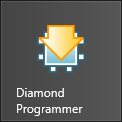
\includegraphics{images/diamond01.png}
  \end{center}
\end{minipage}

\vspace{5mm}

\begin{minipage}{\linewidth}
Stap 2: Maak een nieuw project aan: \\Indien het dialoogvenster ``Programmer: Multiple Cables Detected'' verschijnt, selecteert u het eerste item (``Location 0000'') en klikt u op ``OK''.
  \begin{center}
  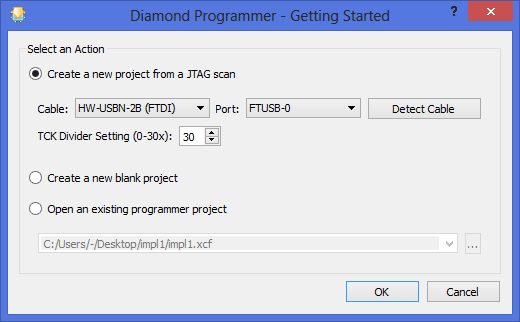
\includegraphics[width=0.7\linewidth]{images/diamond02.png}
  \end{center}
\end{minipage}


\begin{minipage}{\linewidth}
Stap 3: Selecteer kabel: \\U heeft nu een nieuw project aangemaakt dat ``MachXO2'' onder ``Device Family'' en ``LCMXO2-1200HC'' onder ``Device'' zou moeten weergeven.
  \begin{center}
  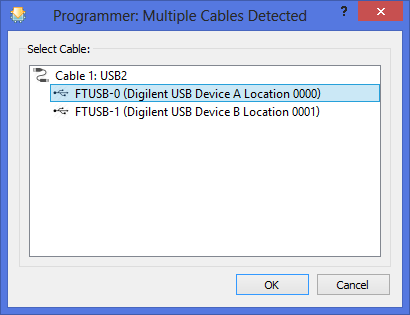
\includegraphics[width=0.6\linewidth]{images/diamond03.png}
  \end{center}
\end{minipage}

\vspace{5mm}

\begin{minipage}{\linewidth}
Stap 4: Nieuw Diamond Programmer-project: \\Kies ``File'' en vervolgens ``Open File'' om het Diamond Programmer-project met de firmware-update voor het MEGA65-toetsenbord te laden.
  \begin{center}
  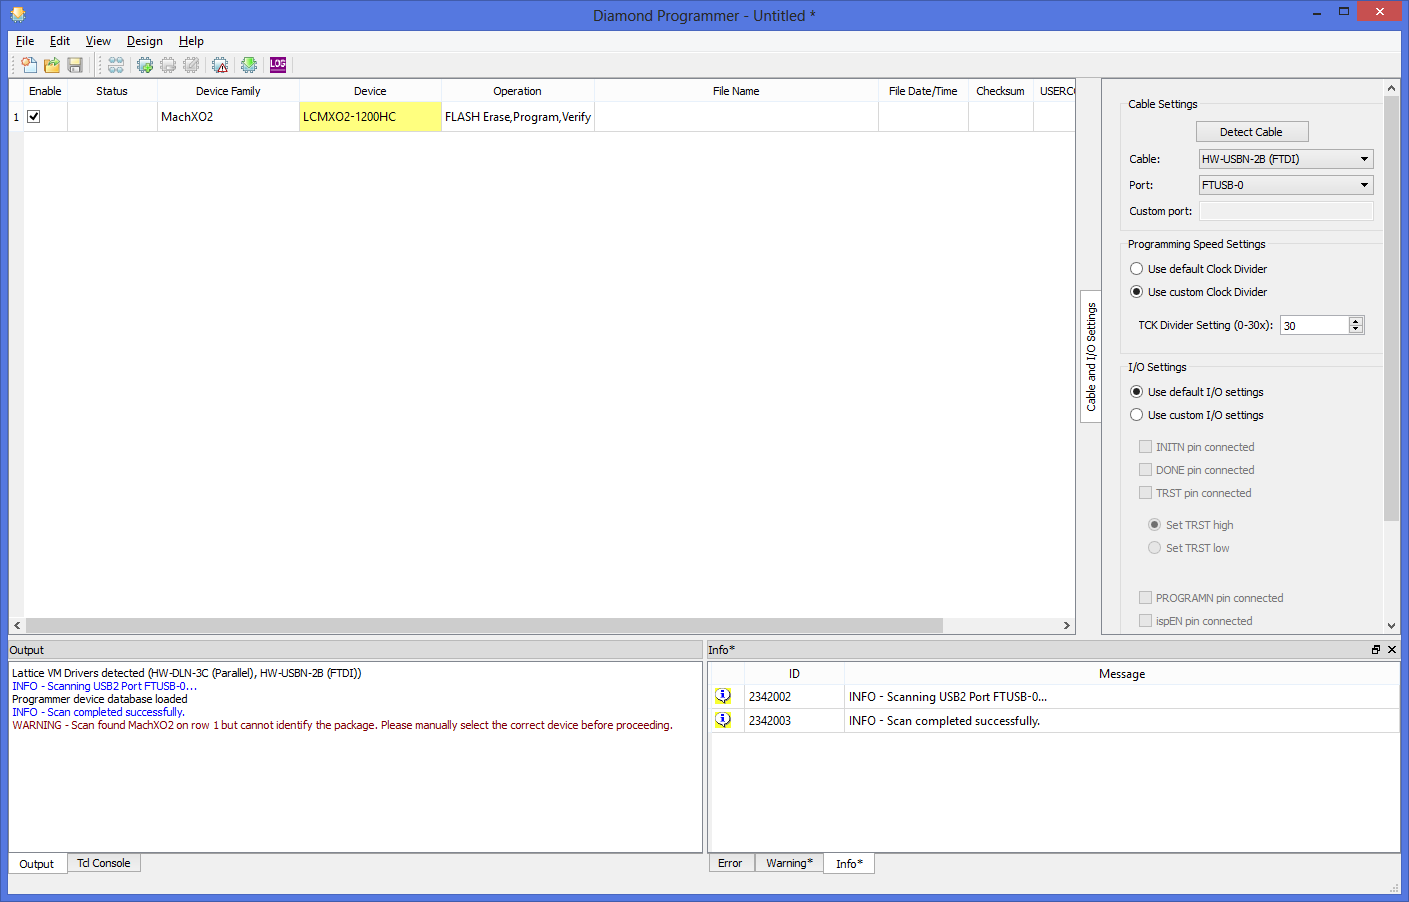
\includegraphics[width=0.8\linewidth]{images/diamond04.png}
  \end{center}
\end{minipage}


\begin{minipage}{\linewidth}
Stap 5: Open project: \\Navigeer naar de map met de uitgepakte firmwarebestanden voor het MEGA65-toetsenbord die u hebt ontvangen en selecteer het bestand met de extensie ``.xcf''.
  \begin{center}
  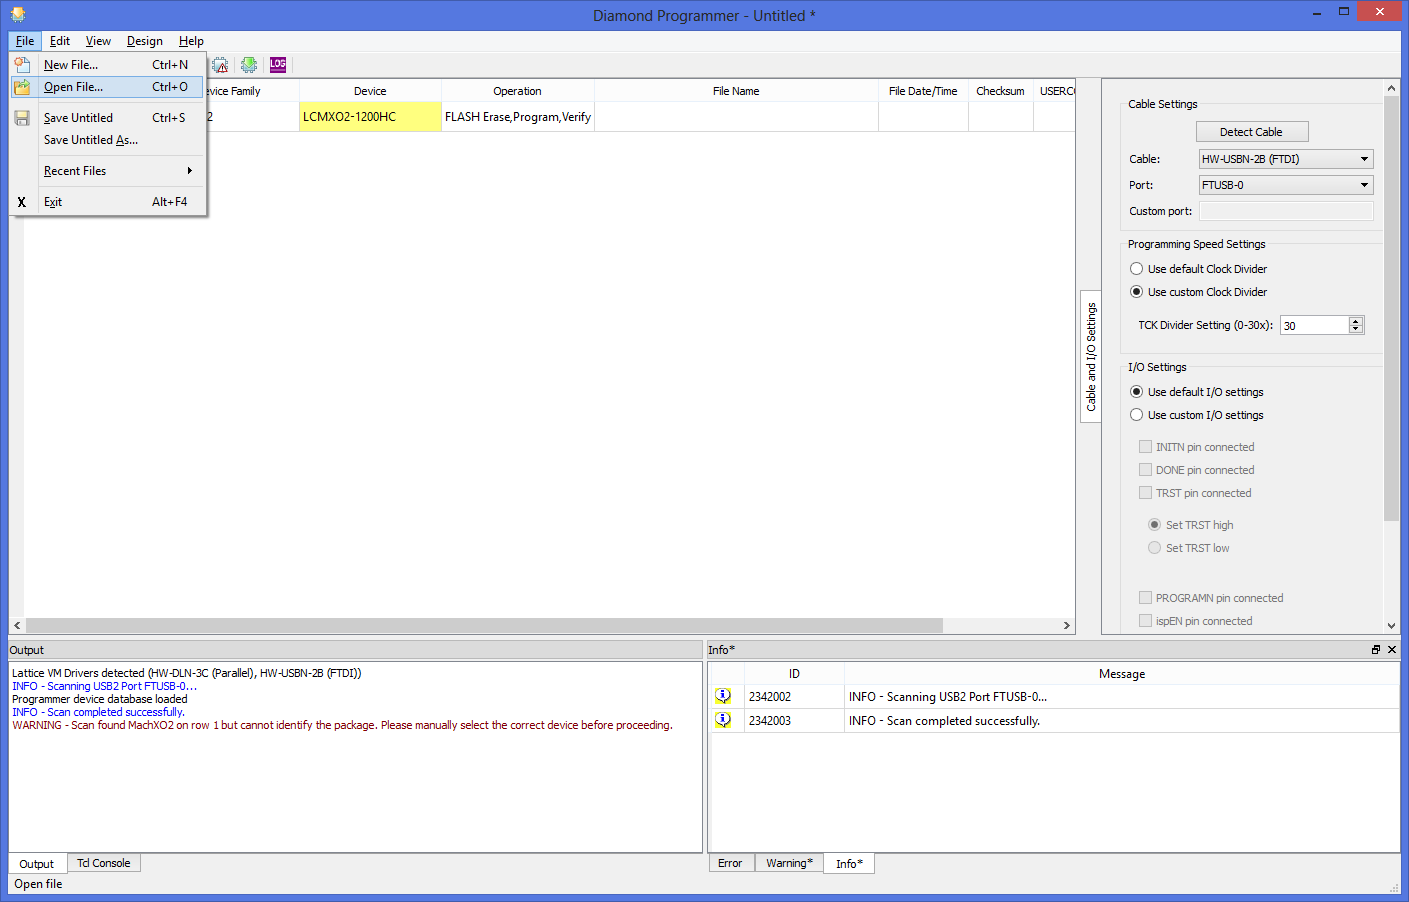
\includegraphics[width=0.8\linewidth]{images/diamond05.png}
  \end{center}
\end{minipage}

\vspace{5mm}

\begin{minipage}{\linewidth}
Stap 6: Selecteer projectbestand: \\Klik op de drie puntjes onder ``File Name'' om het juiste pad in te stellen en het bestand met de extensie ``.jed'' te vinden.
  \begin{center}
  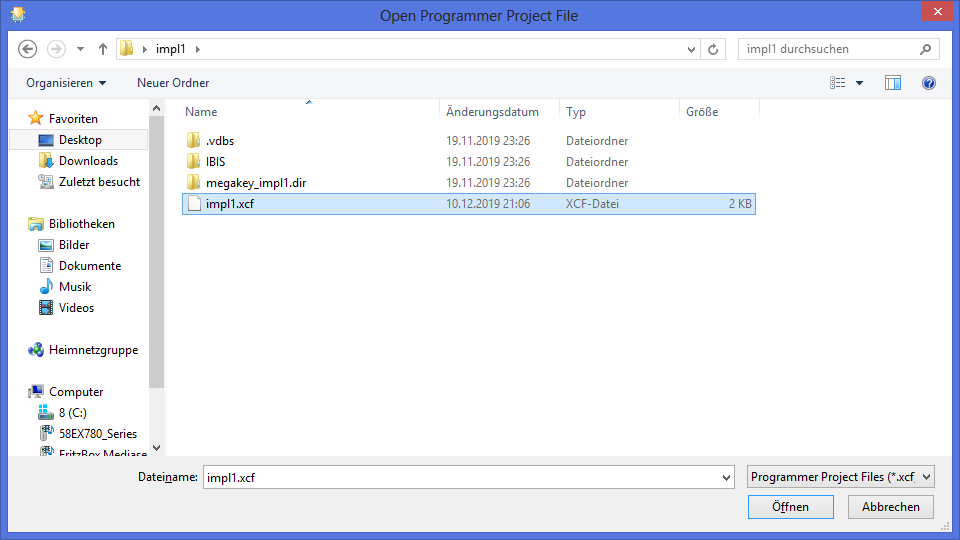
\includegraphics[width=0.8\linewidth]{images/diamond06.png}
  \end{center}
\end{minipage}


\begin{minipage}{\linewidth}
Stap 7: Kies het juiste pad van het .jed-bestand: \\Selecteer het bestand met de extensie ``.jed'' en klik op ``OK''.
  \begin{center}
  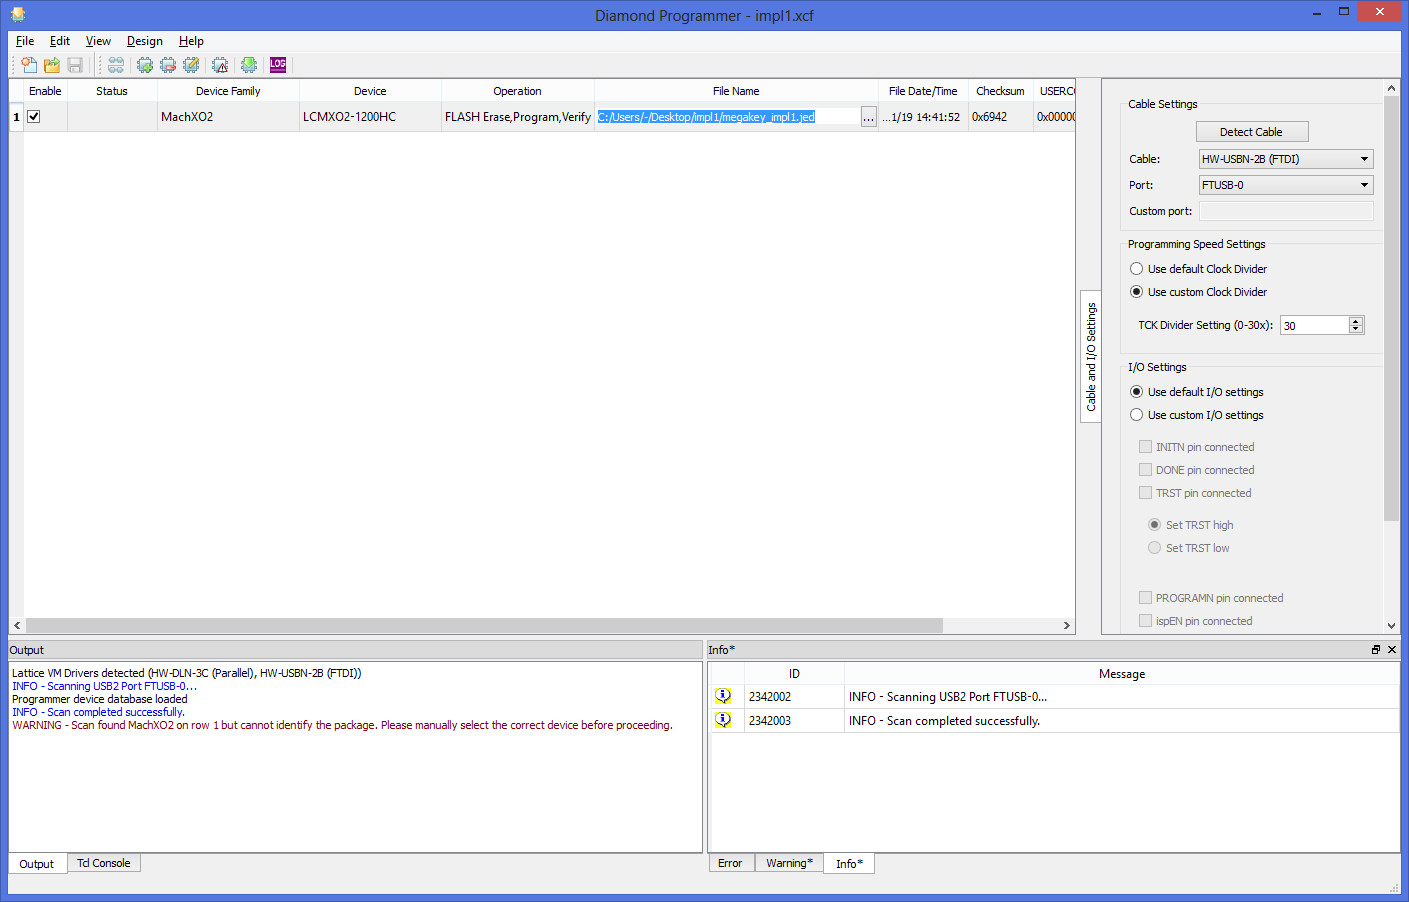
\includegraphics[width=0.8\linewidth]{images/diamond07.png}
  \end{center}
\end{minipage}

\vspace{5mm}

\begin{minipage}{\linewidth}
Stap 8: Selecteer .jed-bestand: \\Klik op het icoon met de groene pijl naar beneden ``PROGRAM'', dat lijkt op het icoon van het Diamond Programmer-programma.
  \begin{center}
  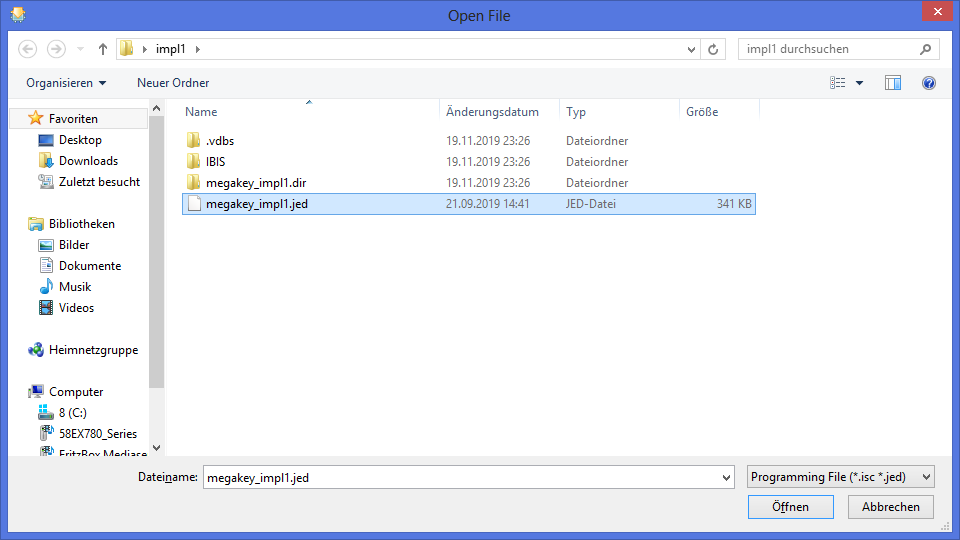
\includegraphics[width=0.8\linewidth]{images/diamond08.png}
  \end{center}
\end{minipage}


\begin{minipage}{\linewidth}
Stap 9: Selecteer kabel: \\Na een moment zou het uitvoervenster ``INFO - Operation: successful.'' moeten weergeven en zou het celletje ``Status'' groen moeten worden (dit gebeurt niet altijd).
  \begin{center}
  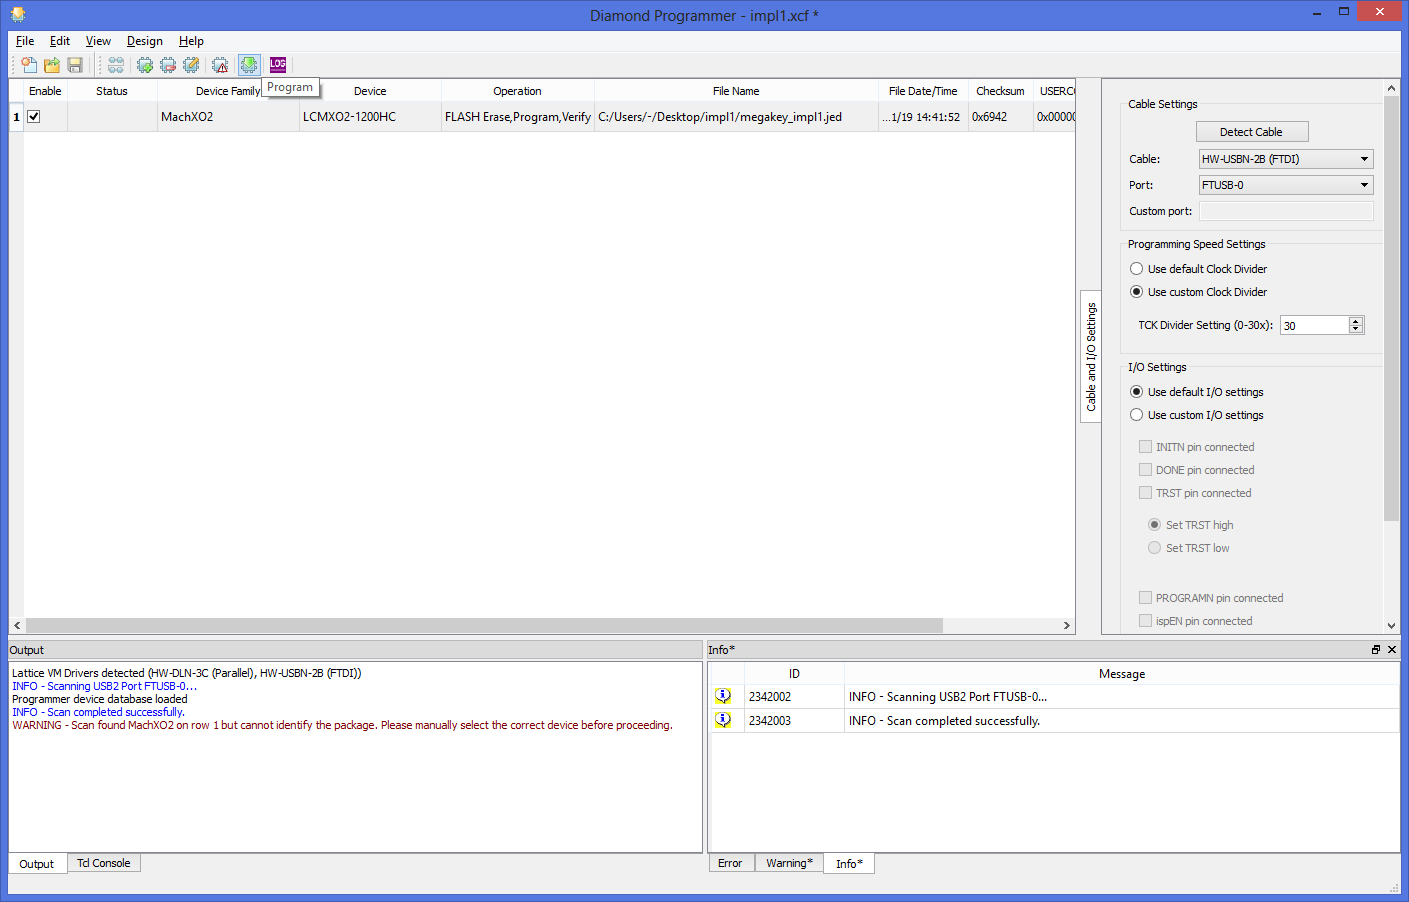
\includegraphics[width=0.8\linewidth]{images/diamond09.png}
  \end{center}
\end{minipage}

\vspace{5mm}

\begin{minipage}{\linewidth}
Stap 10: Operatie geslaagd: \\U heeft het MEGA65-toetsenbord nu succesvol geflasht. Desgewenst kunt u het project opslaan voor later gebruik.
  \begin{center}
  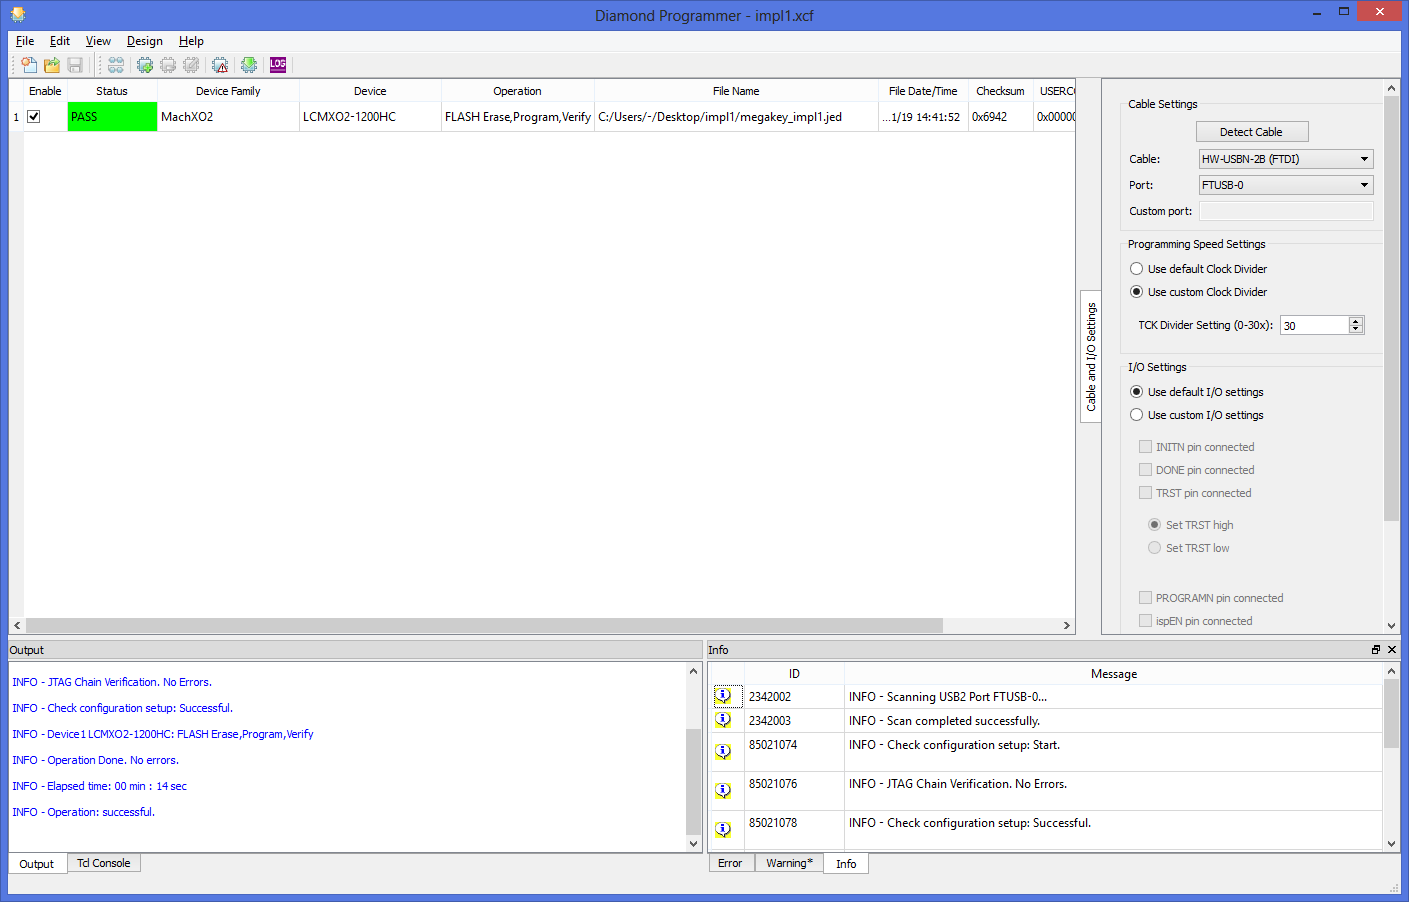
\includegraphics[width=0.8\linewidth]{images/diamond10.png}
  \end{center}
\end{minipage}


\section{Het flashen van de MAX10-FPGA op het MEGA65-moederbord met INTEL QUARTUS}
\label{sec:flashmax10}

Indien u verder wilt gaan, heeft u een TEI0004 - Arrow USB Programmer2-module nodig met het bijbehorende TEI0004-stuurprogramma geïnstalleerd en een goed functionerende installatie van Quartus Prime Programmer Lite Edition. Dit kan zowel op Windows als op Linux, maar in beide gevallen moet u de nodige USB-stuurprogramma's installeren. Sluit de MEGA65 niet aan op de netspanning en installeer de TEI0004 op de J17-connector, die zich tussen de datakabel van de diskette en de ARTIX 7-FPGA op het moederbord bevindt. De micro-USB-poort van de TEI0004 wijst in de tegenovergestelde richting van de HDMI- en LAN-aansluitingen, naar het klepje. De volgende afbeelding toont de juiste positie.

Op het PCB van een R2/R3/R3A/R4-MEGA65-moederbord moeten alle dip-schakelaars in de positie uit staan. De hoofd-FPGA van de MEGA65 mag geen geldige bitstream bevatten. De eenvoudigste manier om dit te bereiken is met een TE0790-JTAG-adapter: u kunt dan het m65-hulpprogramma vanaf een aangesloten computer gebruiken om een bitstream via JTAG te verzenden en vervolgens Control-C gebruiken om het m65-hulpprogramma te onderbreken voordat de bitstream volledig is geladen.

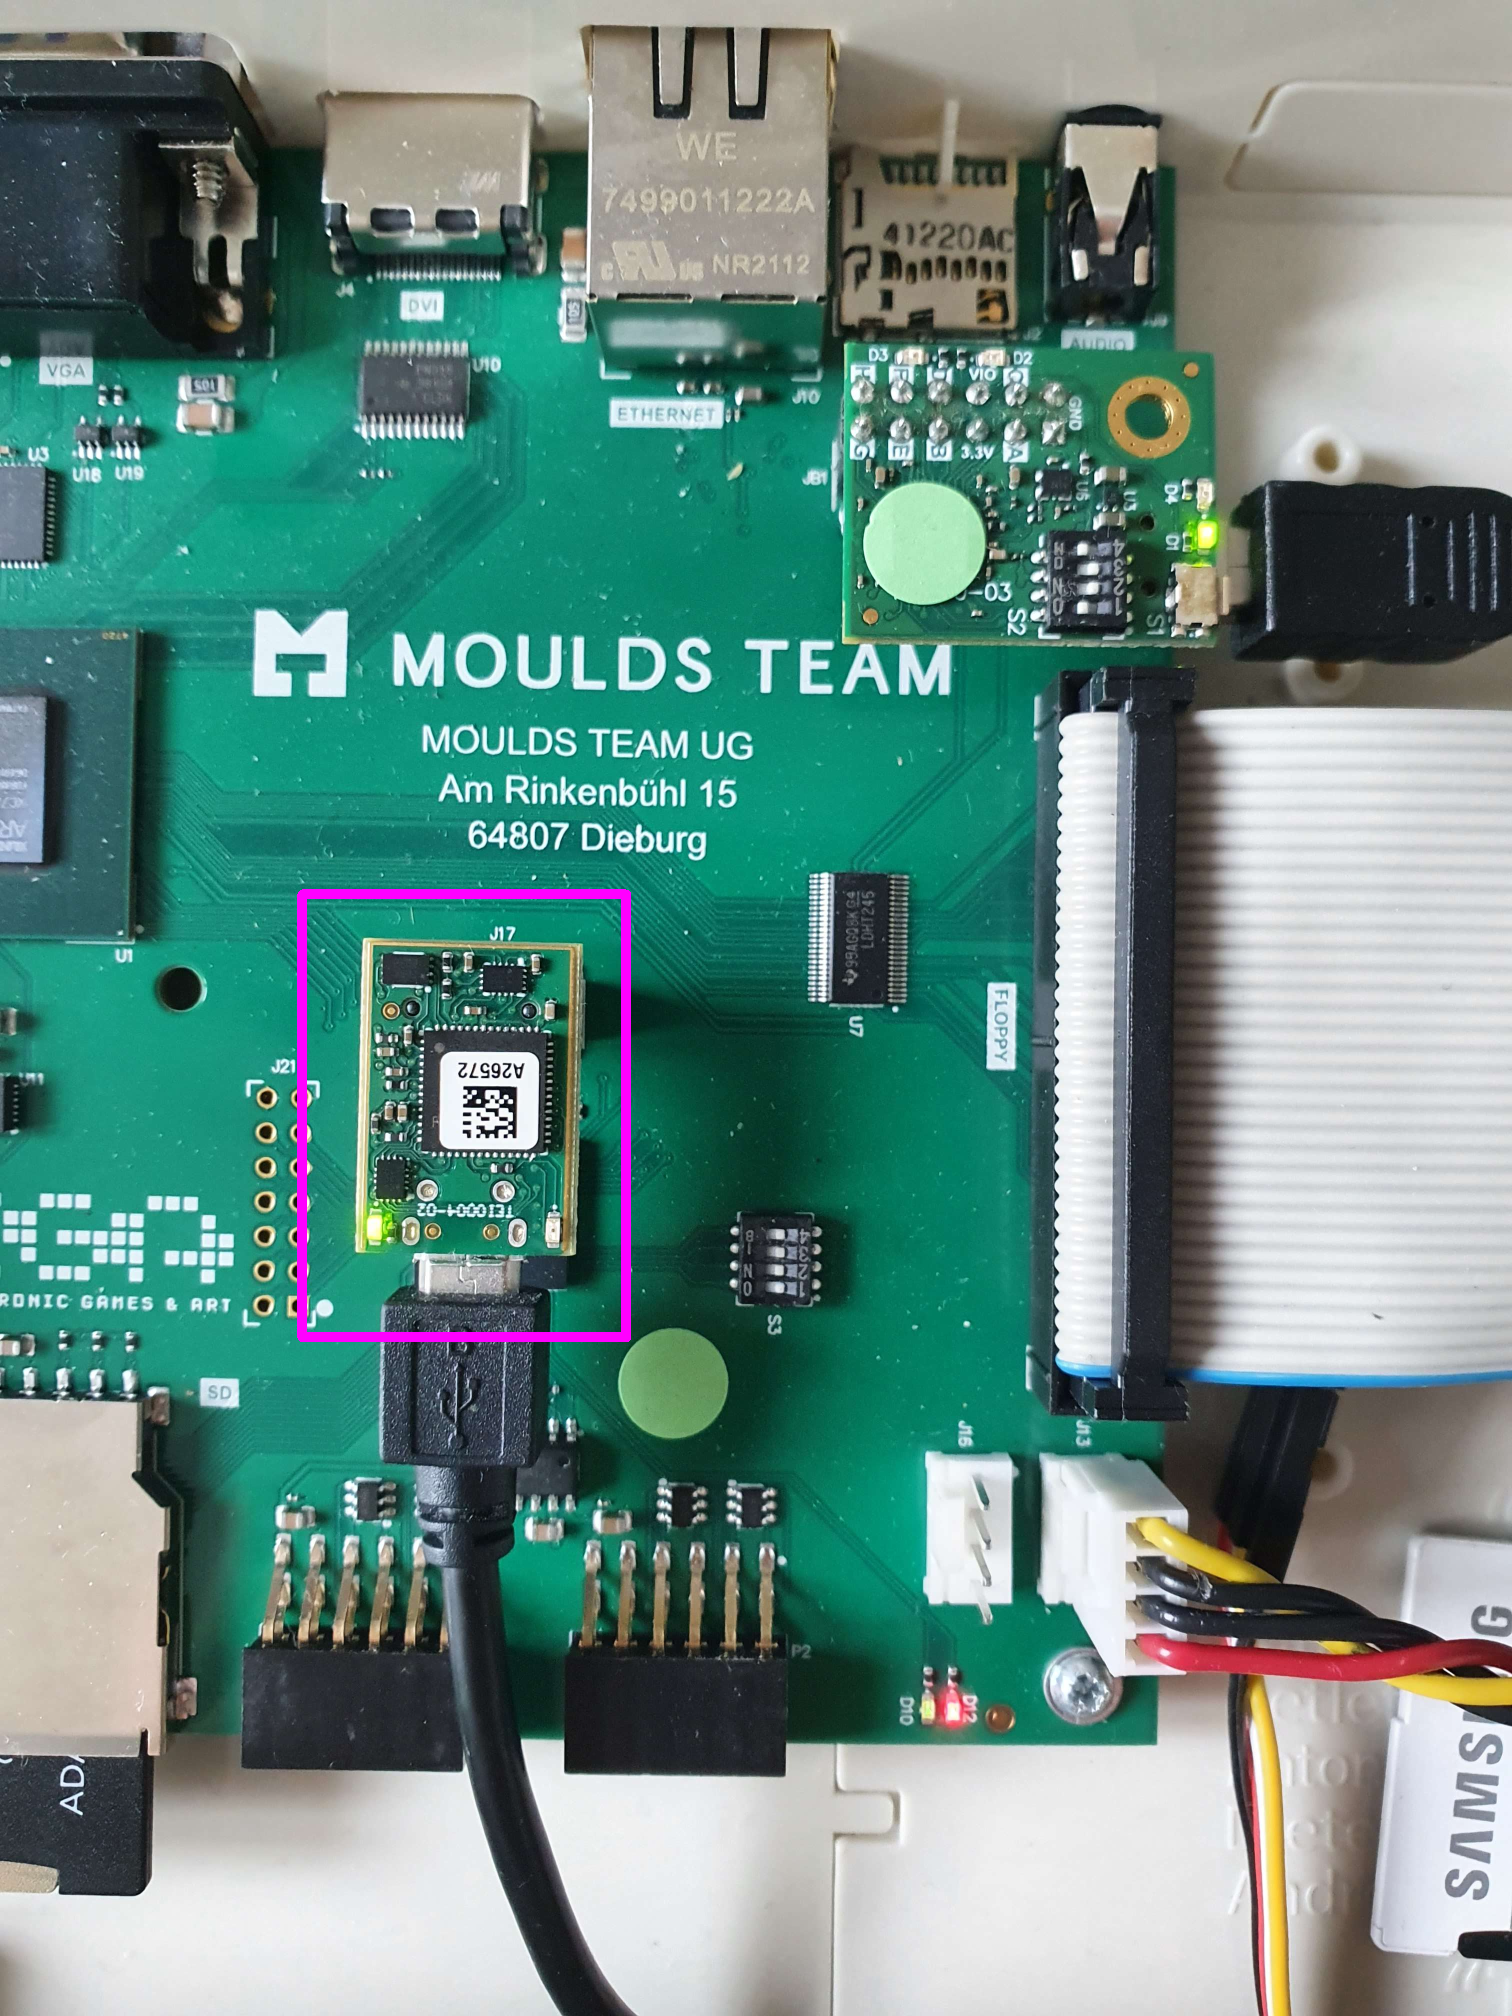
\includegraphics[width=\linewidth]{images/jtag_detail_max10.png}

Sluit uw niet-8-bit computer aan op het FPGA-programmeerapparaat met behulp van een micro-USB-kabel. Open Quartus Prime Programmer Lite Edition, dat van internet kan worden gedownload.

\begin{minipage}{\linewidth}
Stap 1: Open Quartus Prime Programmer Lite Edition: \\Klik op de knop ``Hardware Setup'' in de linkerbovenhoek van het Quartus Prime Programmer-venster.
  \begin{center}
  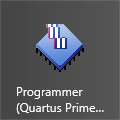
\includegraphics{images/max10_01.png}
  \end{center}
\end{minipage}

\vspace{5mm}

\begin{minipage}{\linewidth}
Stap 2: Hardware-instellingen invoeren: \\In het nieuw verschenen venster kiest u onder ``Currently selected hardware'' voor ``Arrow-USB-Blaster''. Indien ``Arrow-USB-Blaster'' niet verschijnt, controleert u of de kabel en stuurprogramma's correct zijn geïnstalleerd.
  \begin{center}
  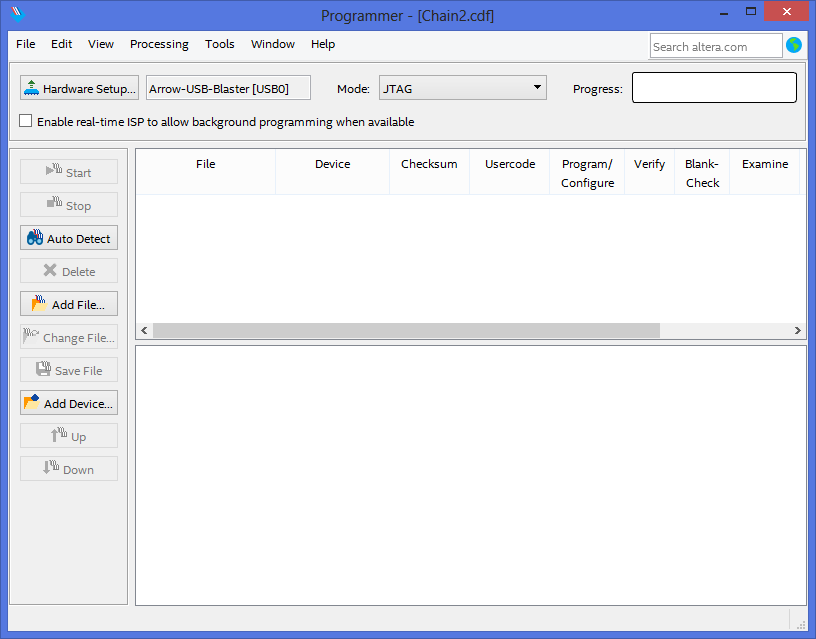
\includegraphics[width=0.8\linewidth]{images/max10_02.png}
  \end{center}
\end{minipage}


\begin{minipage}{\linewidth}
Stap 3: Selecteer Arrow USB-Blaster: \\Klik op de knop ``Add File'' in de linkerrij en kies het nieuwste bestand met de extensie ``.pof''. Klik vervolgens op ``Open''.
  \begin{center}
  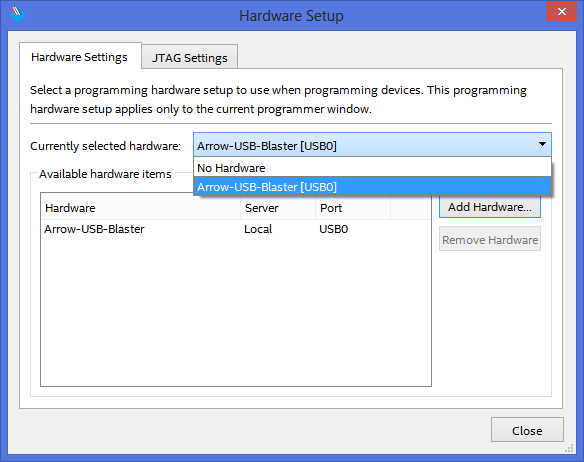
\includegraphics[width=0.8\linewidth]{images/max10_03.png}
  \end{center}
\end{minipage}


\begin{minipage}{\linewidth}
Stap 4: Selecteer programmeerbestand: \\Vink ten minste de drie vakjes onder ``Program/Configure'' aan. Het inschakelen van alle vakjes onder ``Verify'' en ``Blank-Check'' maakt het proces betrouwbaarder.
  \begin{center}
  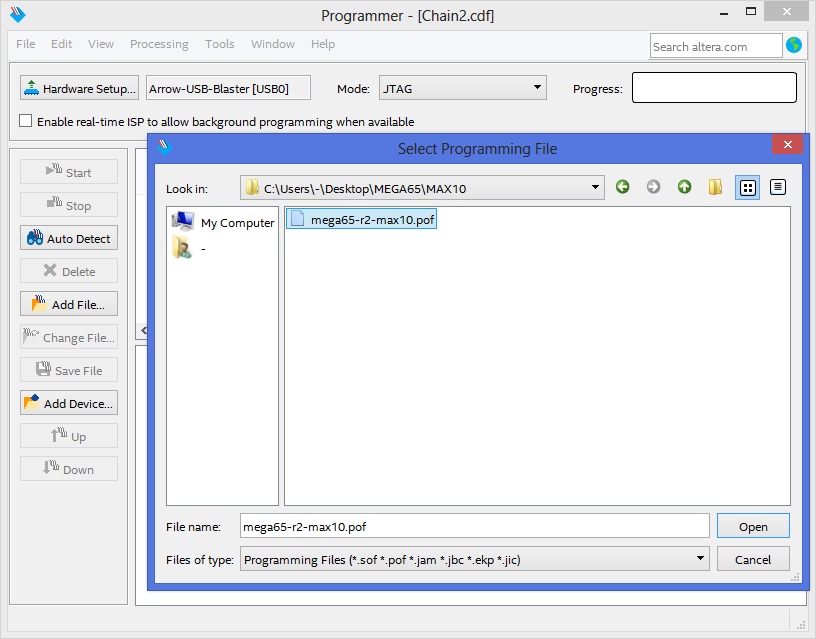
\includegraphics[width=0.7\linewidth]{images/max10_04.png}
  \end{center}
\end{minipage}

\vspace{5mm}

\begin{minipage}{\linewidth}
Stap 5: Selecteer Programmeer-/Configureeropties:
  \begin{center}
  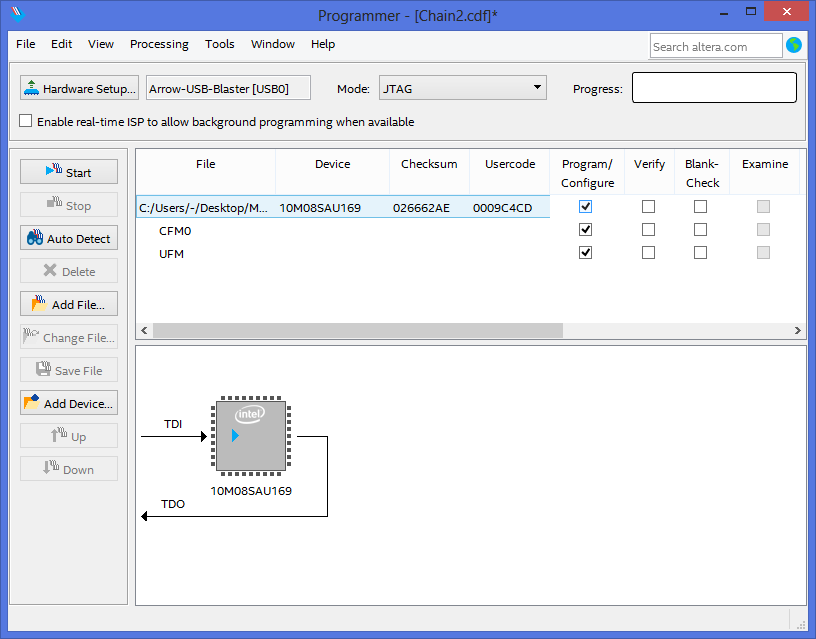
\includegraphics[width=0.7\linewidth]{images/max10_05.png}
  \end{center}
\end{minipage}

Houd de Reset-knop ingedrukt en schakel de MEGA65-computer in. Het toetsenbord gaat in de ``ambulance mode'' (blauwe flitsende lichten). Indien dit niet het geval is, is de hoofd-FPGA niet leeg: start het gehele proces opnieuw.

Klik nu op ``Start'' in de linkerrij van knoppen. De voortgangsbalk rechtsboven zou snel naar 100 procent moeten gaan en groen moeten worden. U heeft de MAX10-FPGA nu succesvol bijgewerkt.

Indien u in plaats daarvan een foutmelding ontvangt, controleer dan of de bitstream van de hoofd-FPGA is gewist en of u de reset-knop op de MEGA65 niet te vroeg heeft losgelaten. Schakel de MEGA65 uit en herhaal deze stap.

\begin{minipage}{\linewidth}
Stap 6: Programmeren geslaagd:
  \begin{center}
  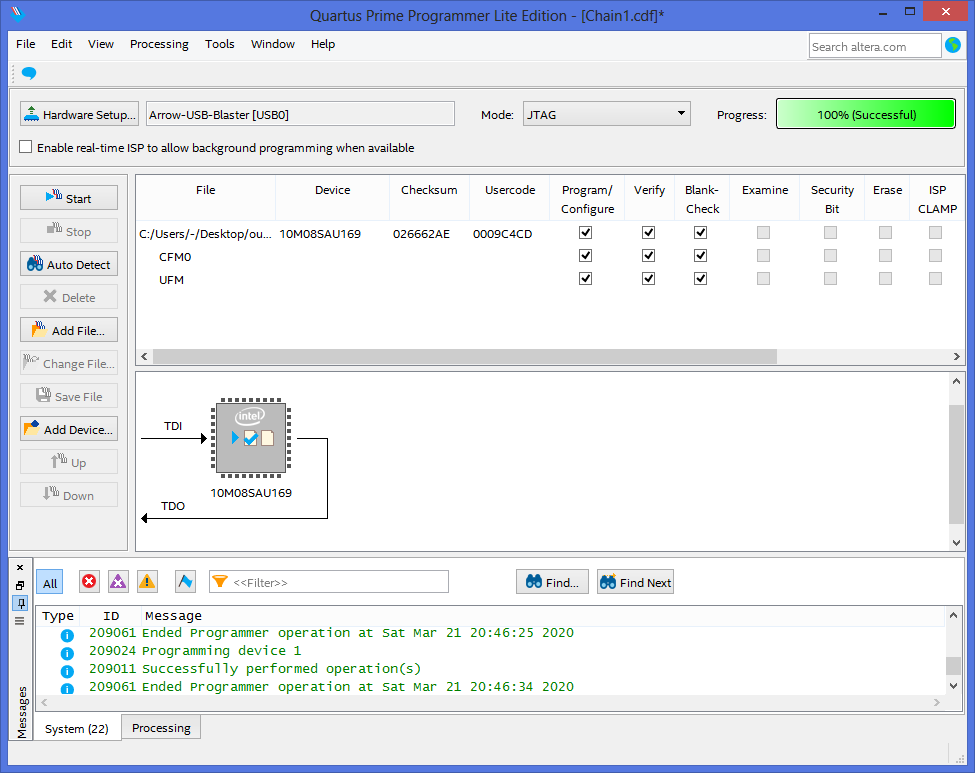
\includegraphics[width=0.8\linewidth]{images/max10_06.png}
  \end{center}
\end{minipage}


  \lstset{
    basicstyle=\small\ttfamily,    columns=flexible,    breaklines=true
}

\chapter{Problemen oplossen}

\section{Hardware}
    \subsection{Geen digitale video-uitvoer}

    \subsubsection{MEGA65 R4, R5, R6}
    De digitale videopoort heeft een verbeterde isolatie tegen terugvoeding gekregen om het probleem ``Geen lampjes bij het inschakelen'' op te lossen.  Een neveneffect hiervan is dat sommige digitale videokabels ten onrechte alleen de behuizing van de connector gebruiken om het grondsignaal door te geven, in plaats van de grondsignalen van de pinnen van de connector te gebruiken.  Kort samengevat: als u geen beeld krijgt op de digitale videopoort, kunt u een van de volgende oplossingen proberen:
    \begin{itemize}
    \item Probeer verschillende digitale videokabels die u heeft.  Dit probleem komt alleen voor bij bepaalde merken kabels, vooral dunnere exemplaren, waarvan wij sterk vermoeden dat de interne grondleidingen ontbreken om kosten te besparen. Dit is de beste oplossing, omdat de kabel daadwerkelijk de oorzaak van het probleem is doordat deze niet aan de specificaties voldoet. Zelfs als u een van de volgende oplossingen toepast, moet u toch op zoek gaan naar een betere HDMI-kabel die het probleem bij de bron oplost.    \item Sluit een VGA-kabel aan op de MEGA65 en op hetzelfde beeldscherm. Hierdoor wordt een grondverbinding via de VGA-connector tot stand gebracht, waardoor de HDMI op mysterieuze wijze plotseling lijkt te werken.    \item Sluit een TE0790 JTAG-adapter aan. Een gebruiker meldde dat dit het probleem eveneens op mysterieuze wijze omzeilde.    \item Verbind de behuizing van de digitale video-connector met de behuizing van de interne SD-kaart op vol formaat.    \item Sluit een splitter of repeater aan op de digitale videopoort.
    \end{itemize}

\begin{figure}
\label{baddvicable}
\caption{Voorbeeld van een slechte (boven) en goede (onder) digitale videokabel. Let op hoe de slechte kabel verdacht dunner is dan de goede. Dit is een teken dat waarschijnlijk dedicated grondleidingen ontbreken, wat problemen veroorzaakt op de MEGA65 R4 en latere revisies.  Elke kabel van ``normale dikte'' zou echter goed moeten werken.  U hoeft geen van die peperdure ``met zilverdraad gevlochten, bij maanlicht door elfen gesmeede'' kabels te kopen.  Die kabels bieden ongeveer evenveel praktisch nut als het strooien van glitter of het tekenen van een eenhoorn aan één uiteinde, maar dan met veel minder klasse.}
\centering
 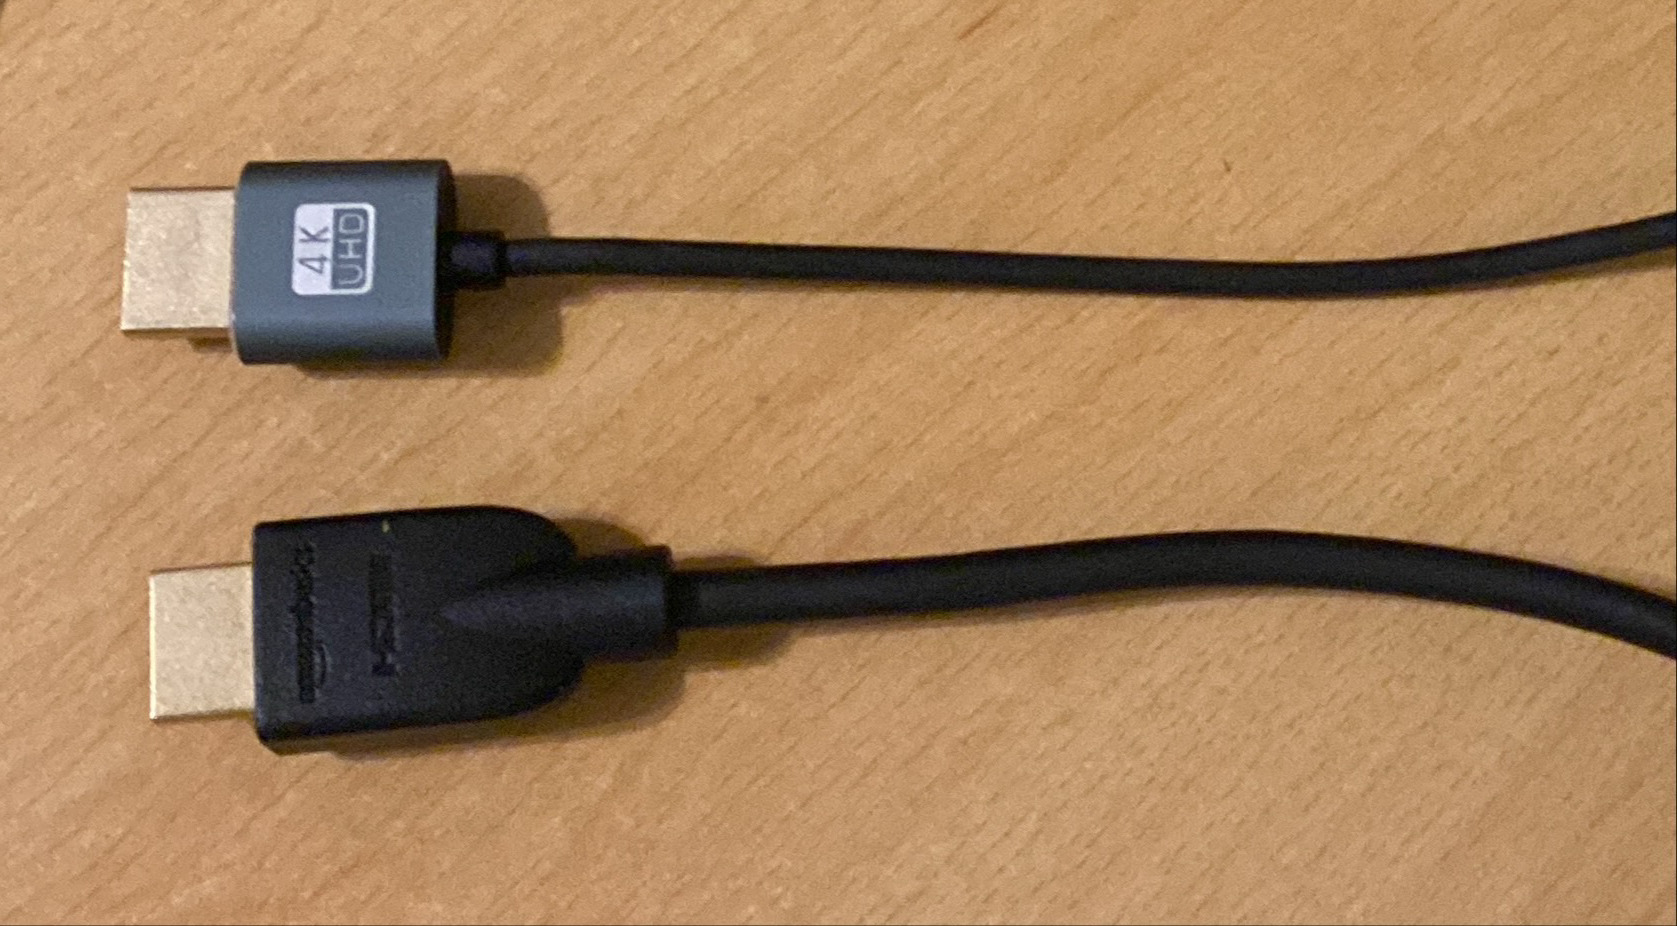
\includegraphics[width=0.7\linewidth]{images/bad-and-good-video-cables.jpg}
\end{figure}

    \subsection{Geen lampjes bij het inschakelen}
    Als de MEGA65 bij het inschakelen soms geen lampjes laat zien, heeft dit te maken met bepaalde digitale video-apparaten die op het moment dat de MEGA65 uitstaat aangesloten zijn en onvoldoende vermogen leveren om de CPLD van het toetsenbord correct van stroom te voorzien, maar wel genoeg om te voorkomen dat deze goed kan resetten wanneer de MEGA65 wordt ingeschakeld. Het verwijderen van de digitale videokabel en het opnieuw inschakelen van het apparaat lost het probleem op.

\section{Vivado}
    \subsection{RAM-vereisten}
    \begin{tcolorbox}[colback=black,coltext=white]
    \begin{lstlisting}
INFO: [Synth 8-256] done synthesizing module 'ram32x1024' [/home/....]
INFO: [Synth 8-256] synthesizing module 'charrom' [/home/....]
    /opt/Xilinx/Vivado/2019.2/bin/loader: line 280: 2317 killed
    WARNING: [Vivado 12-8222] Failed run(s) : 'synth\_1'
        ERROR: Application Exception: failed to launch run 'impl\_1' due to failures in the following run(s):
        synth\_1
        These failed run(s) need to be reset prior to launching 'impl\_1' again.
    \end{lstlisting}
    \end{tcolorbox}
Deze fout wordt veroorzaakt doordat Vivado crasht omdat het apparaat onvoldoende RAM heeft om Vivado uit te voeren.  Vivado heeft minimaal 4 GB RAM nodig om het MEGA65-doel te synthetiseren, maar 8 GB is beter.

\section{mega65\_ftp}
    \subsection{Ontbrekende bibliotheek}
    \begin{tcolorbox}[colback=black,coltext=white]
\begin{lstlisting}
/usr/bin/ld: cannot find -lncurses
collect2: error: ld returned 1 exit status
Makefile:474: recipe for target 'bin/mega65_ftp' failed
make: *** [bin/mega65_ftp] Error 1\end{lstlisting}
    \end{tcolorbox}
Deze fout treedt op wanneer de ncurses-bibliotheek op de computer ontbreekt bij het bouwen van het mega65\_ftp-programma.
Om dit probleem op te lossen, moet u deze afhankelijkheid installeren.

    \begin{tcolorbox}[colback=black,coltext=white]
\begin{lstlisting}
sudo apt-get install libncurses5-dev libncursesw5-dev\end{lstlisting}
    \end{tcolorbox}


  \chapter{Elektronisch schema}
\section{MEGA65 R6 elektronisch schema}
\includepdf[landscape,pages=-,turn=false]{assets/TE0765-06.PDF}
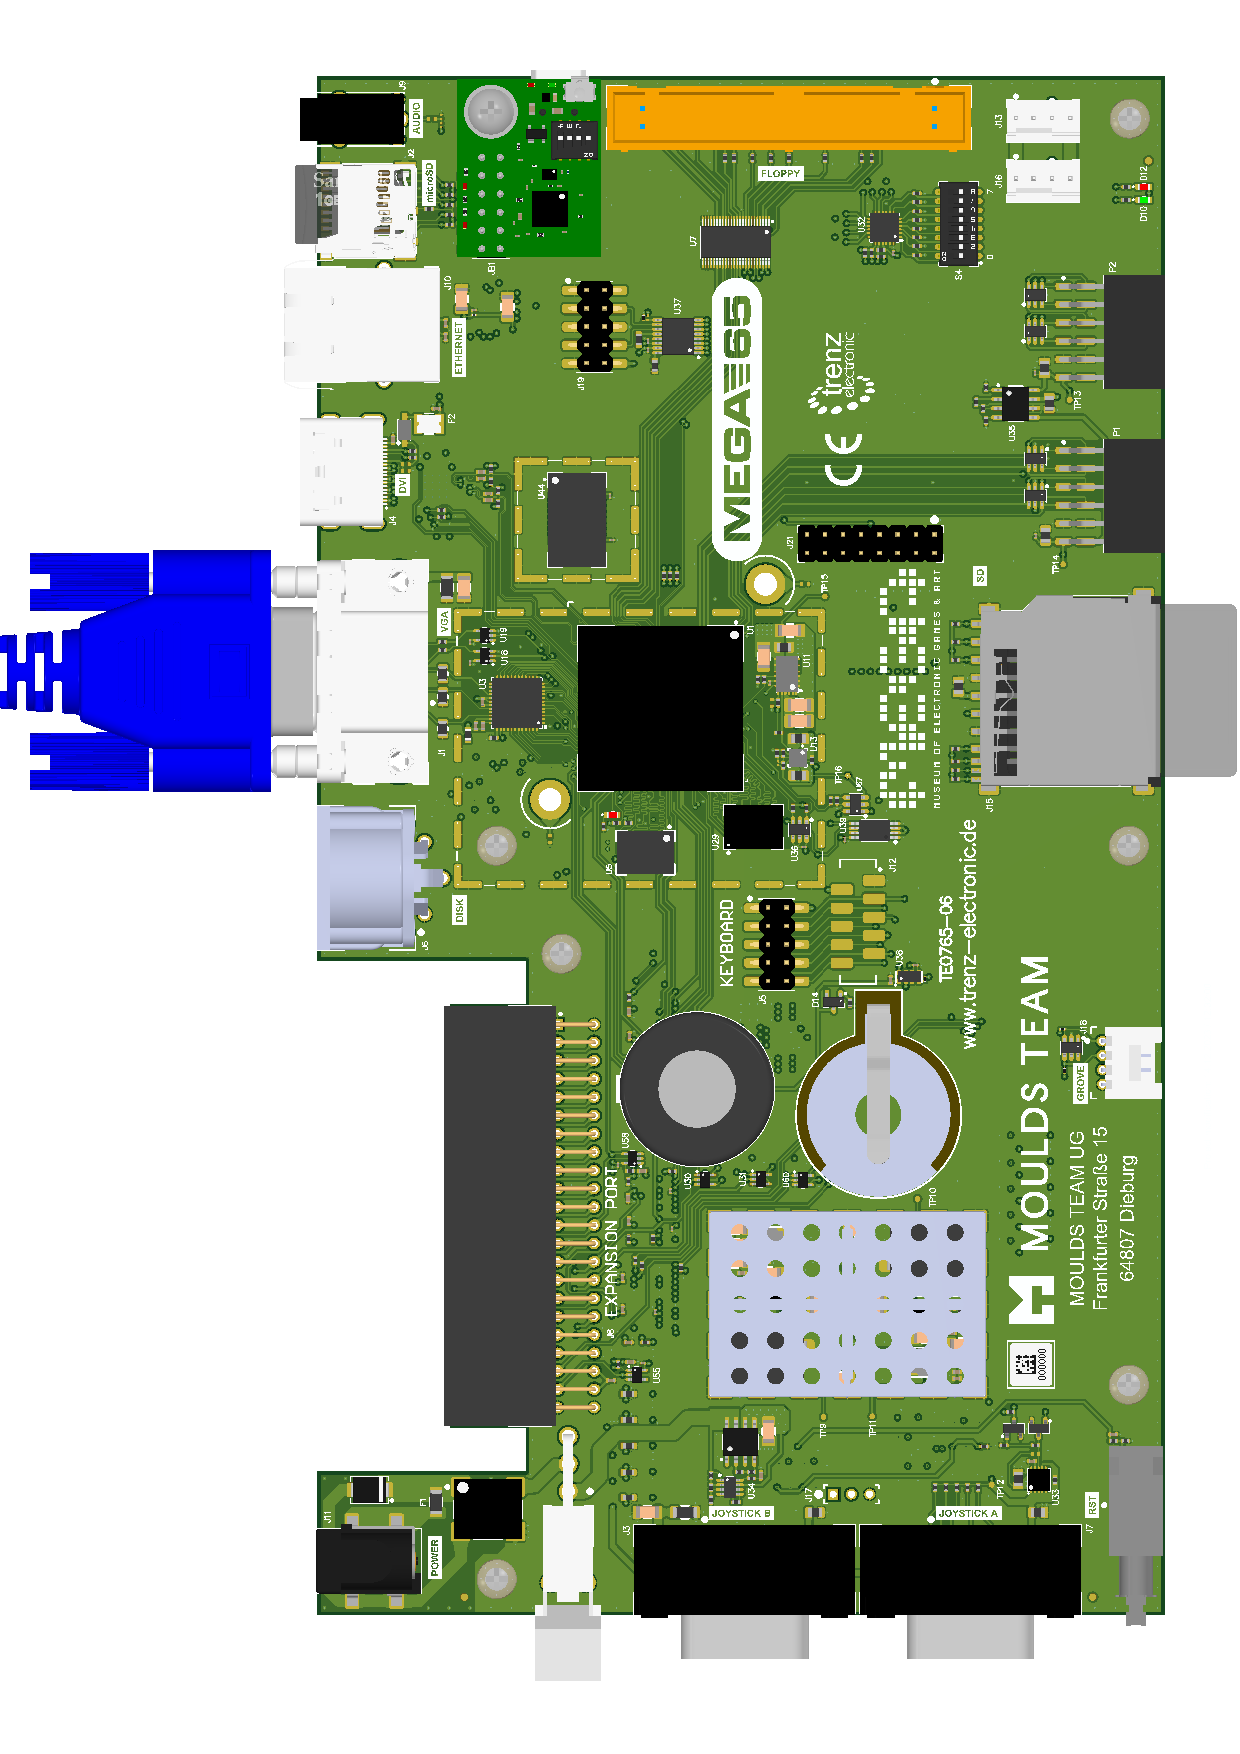
\includepdf[pages=-,turn=false]{assets/TE0765-06-front.PDF}
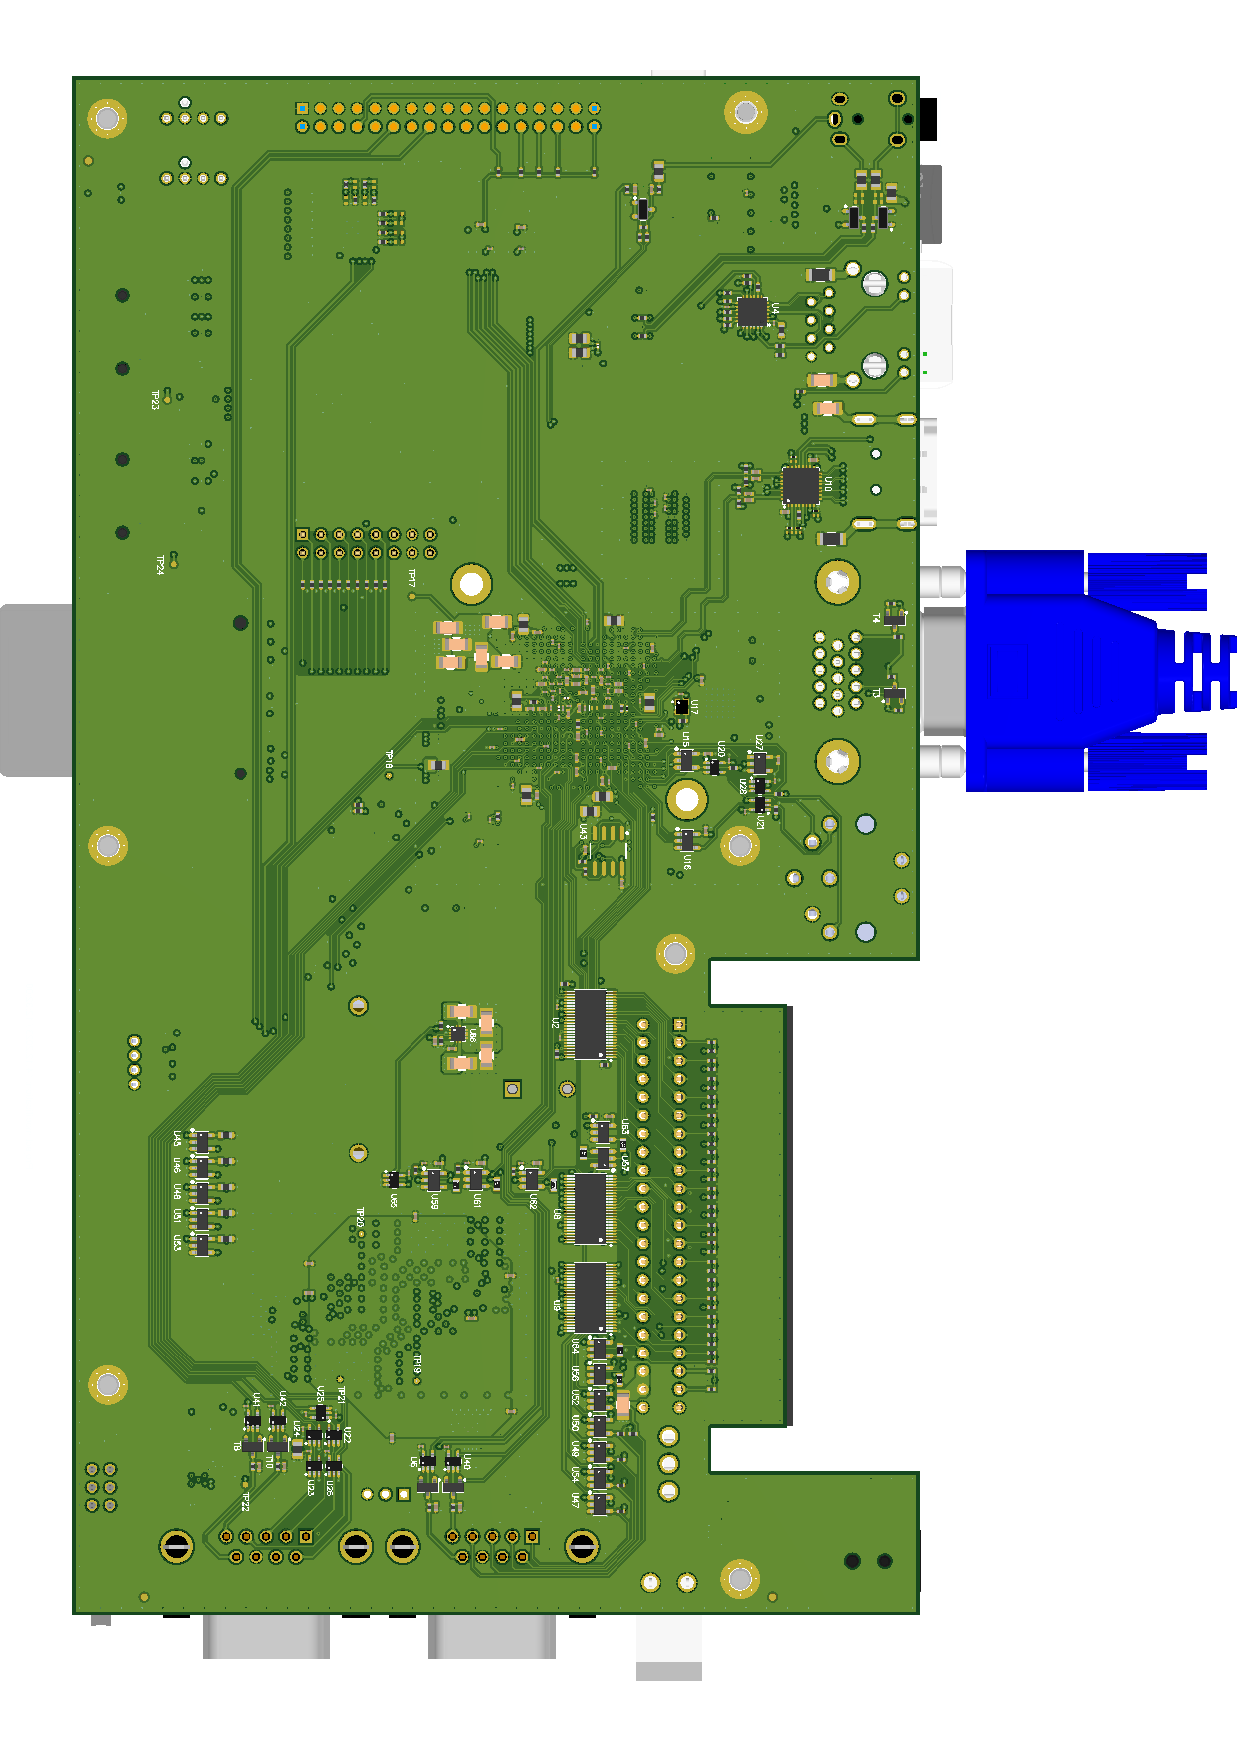
\includepdf[pages=-,turn=false]{assets/TE0765-06-back.PDF}
\section{MEGA65 R3 elektronisch schema}
\includepdf[landscape,pages=-,turn=false]{assets/TE0765-03.PDF}
\section{MEGA65 R2 elektronisch schema}
\includepdf[landscape,pages=-,turn=false]{assets/TE0765-02.PDF}
\section{Nexys Widget Board elektronisch schema}
\label{sec:nexyswidgetschematics}
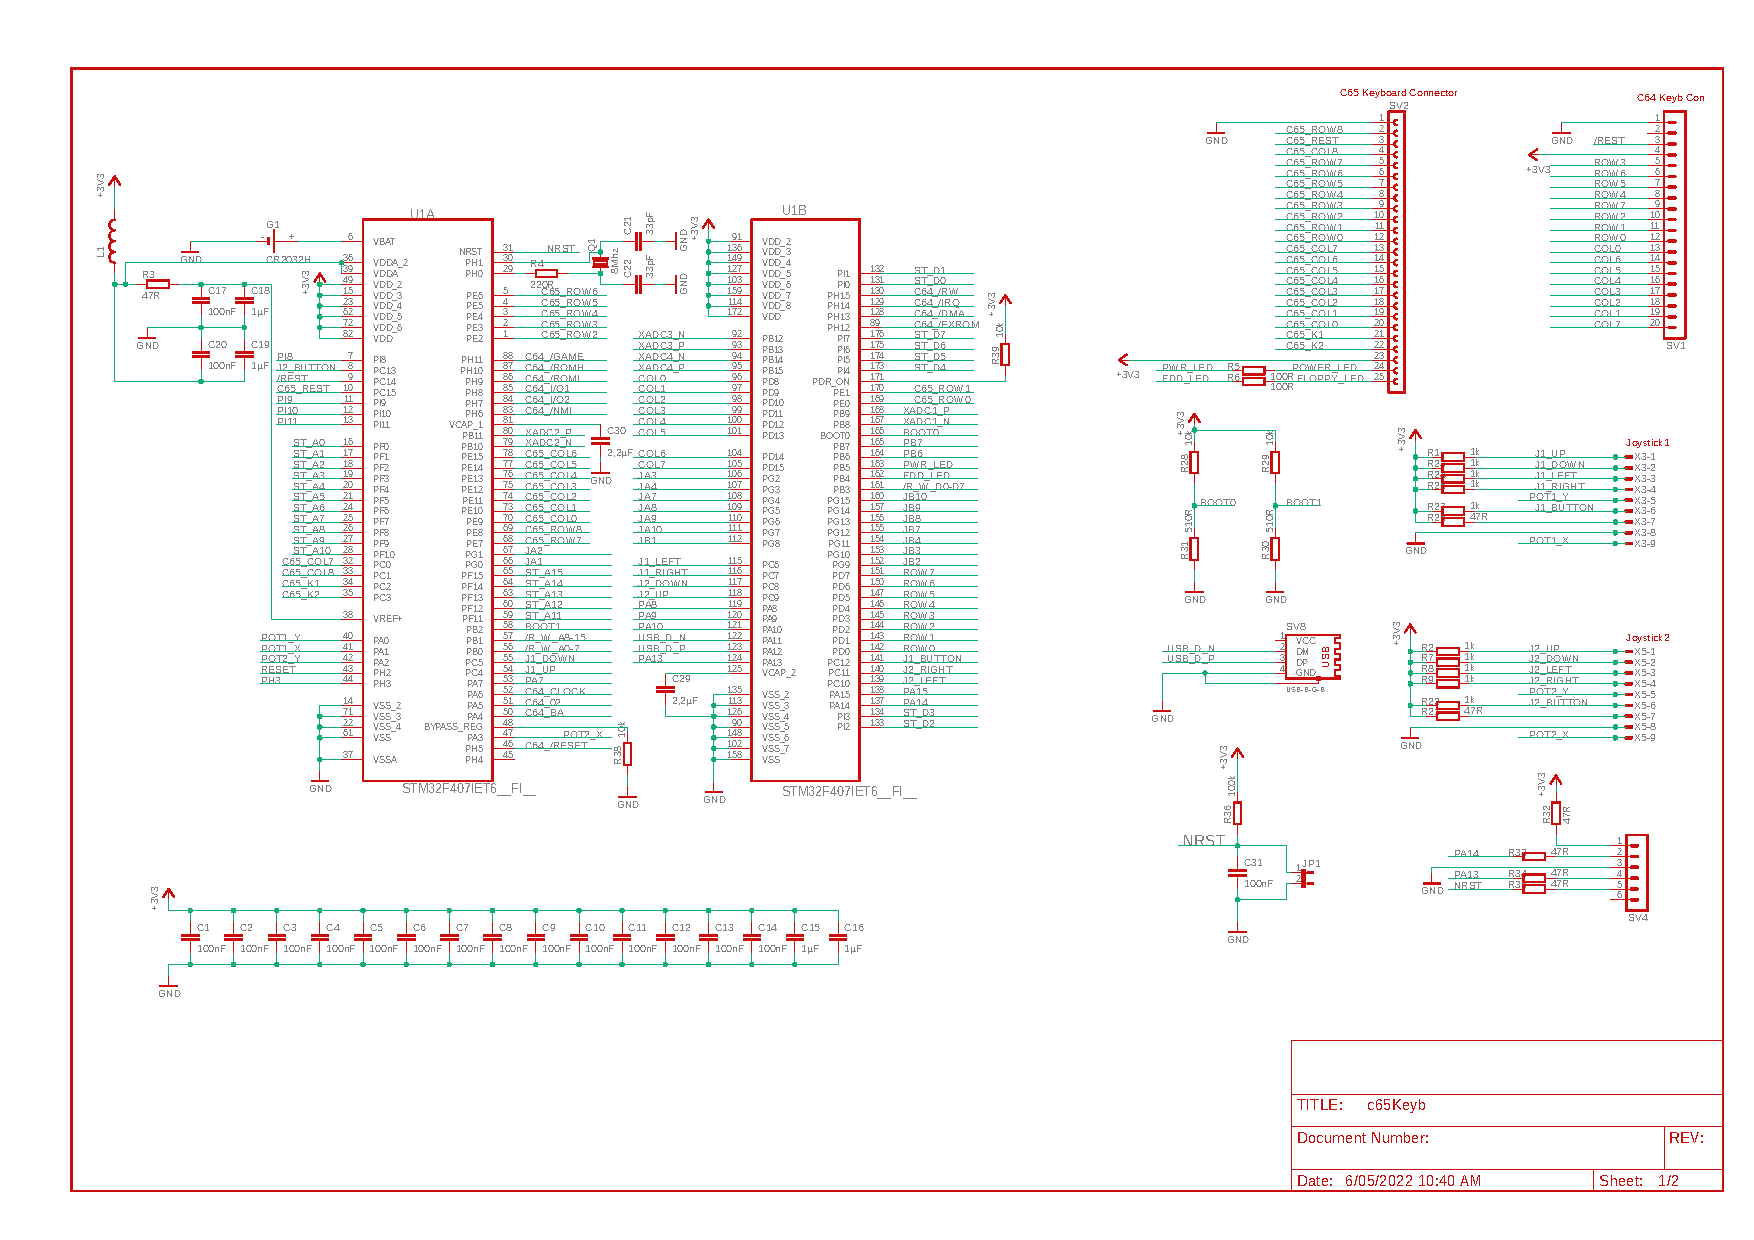
\includepdf[landscape,pages=-,turn=false]{assets/nexys-widget-board-sch.pdf}
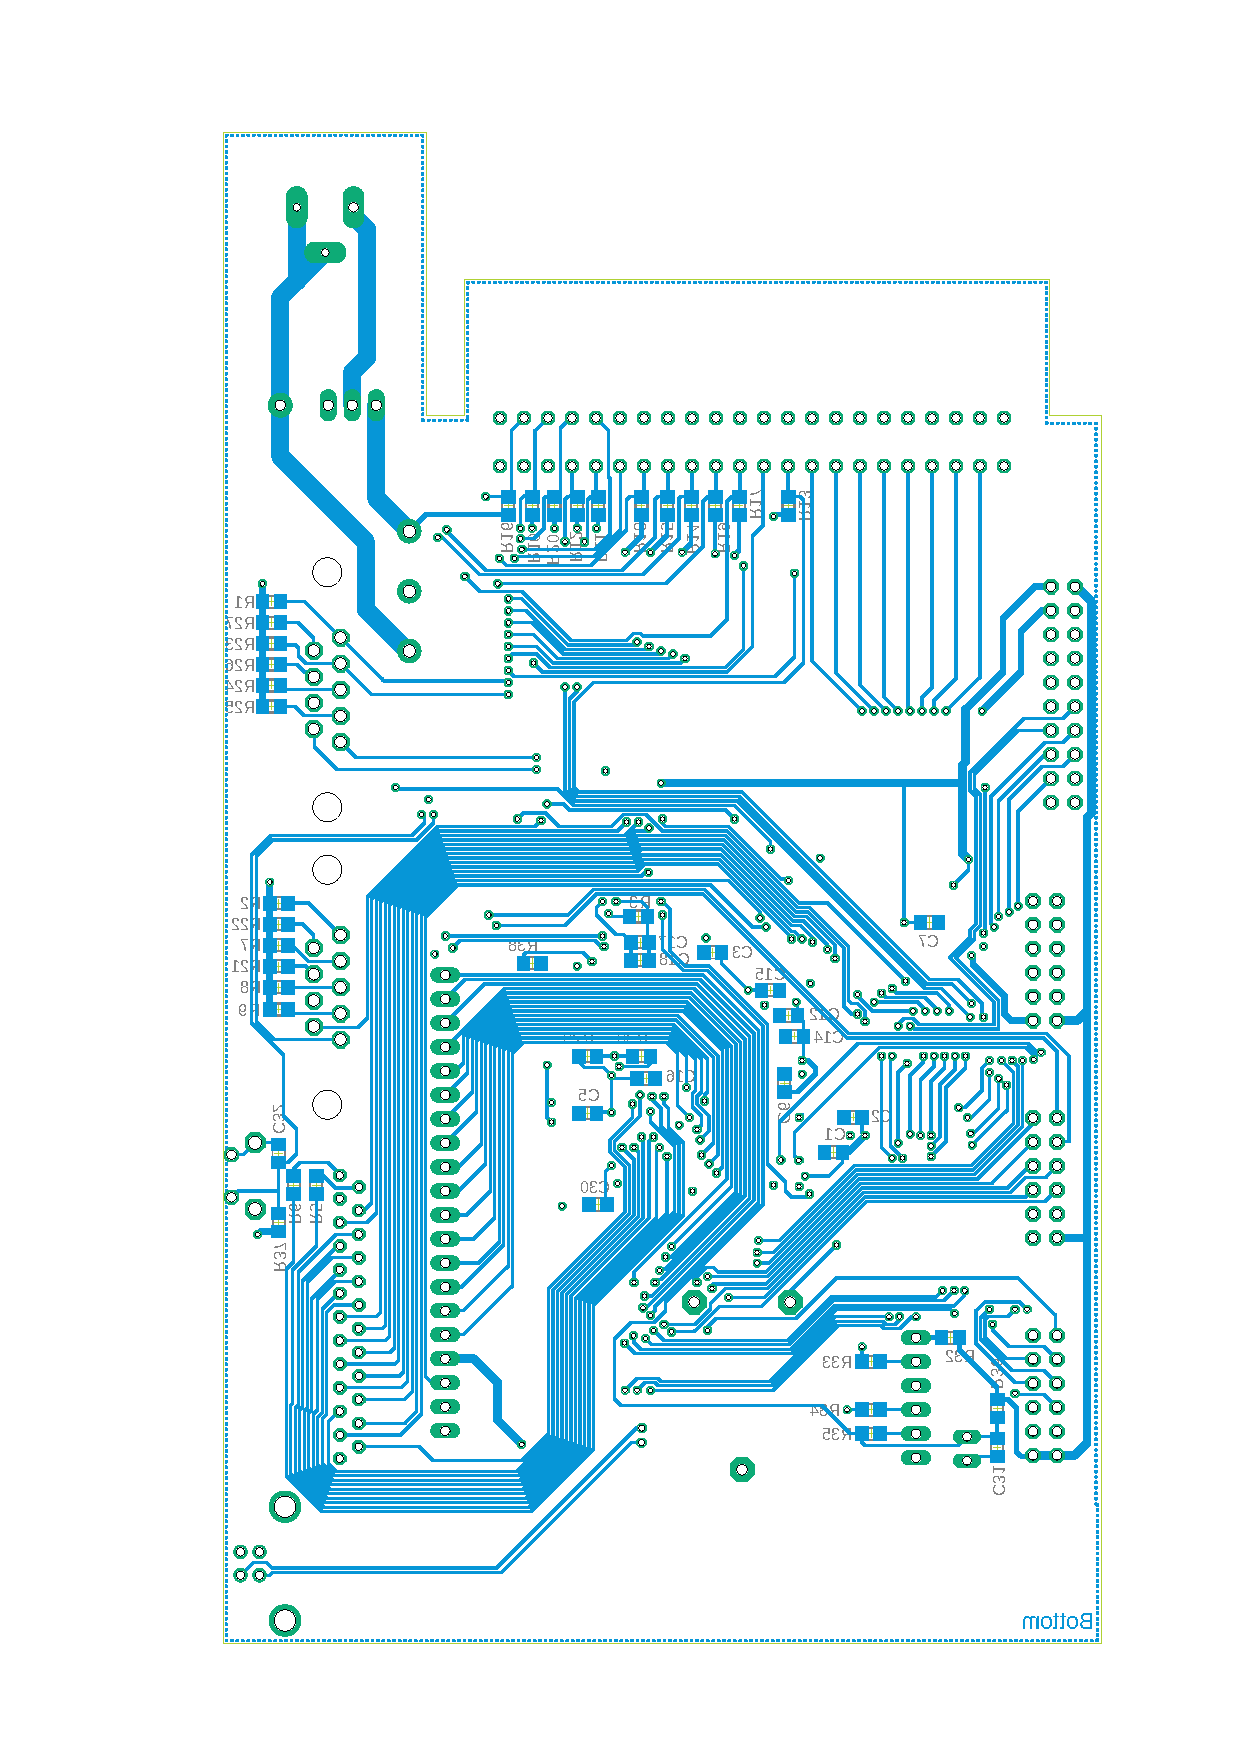
\includepdf[pages=-,turn=false]{assets/nexys-widget-board-pcb.pdf}

  \chapter{Steuners \& donateurs}


De MEGA65 zou niet tot stand zijn gekomen zonder de gulle steun van veel organisaties en individuen.

Wij stellen deze lijsten nog steeds samen; onze excuses indien u er nog niet in voorkomt. Indien u iemand kent die wij over het hoofd hebben gezien, laat het ons dan weten. Zo kunnen wij de bijdrage erkennen van iedereen die de MEGA65 mogelijk heeft gemaakt en die er het geweldige retrocomputingproject van heeft gemaakt dat de computer inmiddels is.

\section{Organisaties}

{\bf Het MEGA Museum of Electronic Games \& Art e.V. Duitsland} \\
\megakey{Alles}

{\bf Trenz Electronic, Duitsland} \\
\megakey{Moederbord}
\megakey{Fabricage}
\megakey{Verkoop}

{\bf Hintsteiner, Oostenrijk} \\
\megakey{Behuizing}

{\bf GMK, Duitsland} \\
\megakey{Toetsenbord}

{\bf KEVAG Telekom, Duitsland} \\
\megakey{Webhosting}

\newpage
\section{Bijdragers}

\begin{mega65thanks}

\begin{minipage}{\linewidth}
  {\large\bf Andreas Liebeskind} \\
  \textit{(libi in paradize)} \\
  Financieel directeur MEGA eV
\end{minipage}

\begin{minipage}{\linewidth}
  {\large\bf Thomas Hertzler} \\
  \textit{(grumpyninja)} \\
  Woordvoerder voor de VS
\end{minipage}

\begin{minipage}{\linewidth}
  {\large\bf Russell Peake} \\
  \textit{(rdpeake)} \\
  Bugherder
\end{minipage}

\begin{minipage}{\linewidth}
  {\large\bf Alexander Nik Petra} \\
  \textit{(n0d)} \\
  Vroeg ontwerp van de behuizing
\end{minipage}

\begin{minipage}{\linewidth}
  {\large\bf Ralph Egas} \\
  \textit{(0-limits)} \\
  Zakelijk adviseur
\end{minipage}

\begin{minipage}{\linewidth}
  {\large\bf Lucas Moss} \\  PCB-ontwerp voor de MEGAphone
\end{minipage}

\begin{minipage}{\linewidth}
  {\large\bf Daren Klamer} \\
  \textit{(Impakt)} \\
  Proeflezen van de handleiding
\end{minipage}

\begin{minipage}{\linewidth}
  {\large\bf Daniël Mantione}  \\
  \textit{(dmantione)} \\
  C64-hardwareguru
\end{minipage}

\columnbreak

\begin{minipage}{\linewidth}
  {\large\bf Dr. Canan Hastik} \\
  \textit{(indica)} \\
  Voorzitter MEGA eV
\end{minipage}

\begin{minipage}{\linewidth}
  {\large\bf Simon Jameson} \\
  \textit{(Shallan)} \\
  Platformverbeteringen
\end{minipage}

\begin{minipage}{\linewidth}
  {\large\bf Stephan Kleinert} \\
  \textit{(ubik)} \\
  Vernietiger van BASIC 10
\end{minipage}

\begin{minipage}{\linewidth}
  {\large\bf Wayne Johnson} \\
  \textit{(sausage)} \\
  Aanvullingen op de handleiding
\end{minipage}

\begin{minipage}{\linewidth}
  {\large\bf Raven L. A. Kleiss} \\
  \textit{(LAK132)} \\
  MegaWAT-presentatiesoftware
\end{minipage}

\begin{minipage}{\linewidth}
  {\large\bf Maurice van Gils }  \\
  \textit{(Maurice)}  \\
  BASIC 65-voorbeeldprogramma's
\end{minipage}

\begin{minipage}{\linewidth}
  {\large\bf Andrew Owen}  \\
  \textit{(Cheveron)} \\
  Toetsenbord, Sinclair-ondersteuning
\end{minipage}

\begin{minipage}{\linewidth}
  {\large\bf Adam Barnes}  \\
  \textit{(amb5l)} \\
  HDMI-expert en printplaatherziening
\end{minipage}

\begin{minipage}{\linewidth}
  {\large\bf Wayne Rittimann, Jr.} \\
  \textit{(johnwayner)} \\
  Bugverplettering op alle niveaus
\end{minipage}

\end{mega65thanks}


\newpage
\section{Steuners}

\begin{small}
% page 1
\setlength{\tabcolsep}{1mm}
\begin{tabular}{p{4cm}p{4cm}p{4cm}}
3c74ce64 & Arne Neumann & Christian Gräfe \\8-Bit Classics & Arne Richard Tyarks & Christian Heffner \\@11110110100 & Axel Klahr & Christian Kersting \\Aaron Smith & Balaz Ondrej & Christian Schiller \\Achim Mrotzek & Barry Thompson & Christian Streck \\Adolf Nefischer & Bartol Filipovic & Christian Weyer \\Adrian Esdaile & Benjamin Maas & Christian Wyk \\Adrien Guichard & Bernard Alaiz & Christoph Haug \\Ahmed Kablaoui & Bernhard Zorn & Christoph Huck \\Alan Bastian Witkowski & Bieno Marti-Braitmaier & Christoph Pross \\Alan Field & Bigby & Christopher Christopher \\Alastair Paulin-Campbell & Bill LaGrue & Christopher Kalk \\Alberto Mercuri & Bjoerg Stojalowski & Christopher Kohlert \\Alexander Haering & Björn Johannesson & Christopher Nelson \\Alexander Kaufmann & Bjørn Melbøe & Christopher Taylor \\Alexander Niedermeier & Bo Goeran Kvamme & Christopher Whillock \\Alexander Soppart & Boerge Noest & Claudio Piccinini \\Alfonso Ardire & Bolko Beutner & Claus Skrepek \\Amiga On The Lake & Brett Hallen & Collen Blijenberg \\André Kudra & Brian Gajewski & Constantine Lignos \\André Simeit & Brian Green & Crnjaninja \\André Wösten & Brian Juul Nielsen & Daniel Auger \\Andrea Farolfi & Brian Reiter & Daniel Julien \\Andrea Minutello & Bryan Pope & Daniel Lobitz \\Andreas Behr & Burkhard Franke & Daniel O'Connor \\Andreas Freier & Byron Goodman & Daniel Teicher \\Andreas Grabski & Cameron Roberton (KONG) & Daniel Tootill \\Andreas Millinger & Carl Angervall & Daniel Wedin \\Andreas Nopper & Carl Danowski & Daniele Benetti \\Andreas Ochs & Carl Stock & Daniele Gaetano Capursi \\Andreas Wendel Manufaktur & Carl Wall & Dariusz Szczesniak \\Andreas Zschunke & Carlo Pastore & Darrell Westbury \\Andrew Bingham & Carlos Silva & David Asenjo Raposo \\Andrew Dixon & Carsten Sørensen & David Dillard \\Andrew Mondt & Cenk Miroglu Miroglu & David Gorgon \\Andrzej Hłuchyj & Chang sik Park & David Norwood \\Andrzej Sawiniec & Charles A. Hutchins Jr. & David Raulo \\Andrzej Śliwa & Chris Guthrey & David Ross \\Anthony W. Leal & Chris Hooper & de voughn accooe \\Arkadiusz Bronowicki & Chris Stringer & Dean Scully \\Arkadiusz Kwasny & Christian Boettcher & Dennis Jeschke \\Arnaud Léandre & Christian Eick & Dennis Schaffers \\Arne Drews & Christian Gleinser & Dennis Schierholz \\
\end{tabular}
% page 2
\newpage
\setlength{\tabcolsep}{1mm}
\begin{tabular}{p{4cm}p{4cm}p{4cm}}
Dennis Schneck & Frank Haaland & Helge Förster \\denti & Frank Hempel & Hendrik Fensch \\Dick van Ginkel & Frank Koschel & Henning Harperath \\Diego Barzon & Frank Linhares & Henri Parfait \\Dierk Schneider & Frank Sleeuwaert & Henrik Kühn \\Dietmar Krueger & Frank Wolf & Holger Burmester \\Dietmar Schinnerl & FranticFreddie & Holger Sturk \\Dirk Becker & Fredrik Ramsberg & Howard Knibbs \\Dirk Wouters & Fridun Nazaradeh & Hubert de Hollain \\Domingo Fivoli & Friedel Kropp & Huberto Kusters \\DonChaos & Garrick West & Hugo Maria Gerardus v.d. Aa \\Donn Lasher & Gary Lake-Schaal & Humberto Castaneda \\Douglas Johnson & Gary Pearson & Ian Cross \\Dr. Leopold Winter & Gavin Jones & IDE64 Staff \\Dusan Sobotka & Geir Sigmund Straume & Igor Ianov \\Earl Woodman & Gerd Mitlaender & Igor Kurtes \\Ed Reilly & Giampietro Albiero & Immo Beutler \\Edoardo Auteri & Giancarlo Valente & Ingo Katte \\Eduardo Gallardo & Gianluca Girelli & Ingo Keck \\Eduardo Luis Arana & Giovanni Medina & Insanely Interested Publishing \\Eirik Juliussen Olsen & Glen Fraser & IT-Dienstleistungen Obsieger \\Emilio Monelli & Glen R Perye III & Ivan Elwood \\EP Technical Services & Glenn Main & Jaap HUIJSMAN \\Epic Sound & Gordon Rimac & Jace Courville \\Erasmus Kuhlmann & GRANT BYERS & Jack Wattenhofer \\ergoGnomik & Grant Louth & Jakob Schönpflug \\Eric Hilaire & Gregor Bubek & Jakub Tyszko \\Eric Hildebrandt & Gregor Gramlich & James Hart \\Eric Hill & Guido Ling & James Marshburn \\Eric Jutrzenka & Guido von Gösseln & James McClanahan \\Erwin Reichel & Guillaume Serge & James Sutcliffe \\Espen Skog & Gunnar Hemmerling & Jan Bitruff \\Evangelos Mpouras & Günter Hummel & Jan Hildebrandt \\Ewan Curtis & Guy Simmons & Jan Iemhoff \\Fabio Zanicotti & Guybrush Threepwood & Jan Kösters \\Fabrizio Di Dio & Hakan Blomqvist & Jan Peter Borsje \\Fabrizio Lodi & Hans Pronk & Jan Schulze \\FARA Gießen GmbH & Hans-Jörg Nett & Jan Stoltenberg-Lerche \\FeralChild & Hans-Martin Zedlitz & Janne Tompuri \\First Choice Auto's & Harald Dosch & Jannis Schulte \\Florian Rienhardt & Harri Salokorpi & Jari Loukasmäki \\Forum64. de & Harry Culpan & Jason Smith \\Francesco Baldassarri & Harry Venema & Javier Gonzalez Gonzalez \\Frank Fechner & Heath Gallimore & Jean-Paul Lauque \\Frank Glaush & Heinz Roesner & Jeffrey van der Schilden \\Frank Gulasch & Heinz Stampfli & Jens Schneider \\
\end{tabular}
% page 3
\newpage
\setlength{\tabcolsep}{1mm}
\begin{tabular}{p{4cm}p{4cm}p{4cm}}
Jens-Uwe Wessling & Kenneth Joensson & Marco Cappellari \\Jesse DiSimone & Kevin Edwards & Marco Rivela \\Jett Adams & Kevin Thomasson & Marco van de Water \\Johan Arneklev & Kim Jorgensen & Marcus Gerards \\Johan Berntsson & Kim Rene Jensen & Marcus Herbert \\Johan Svensson & Kimmo Hamalainen & Marcus Linkert \\Johannes Fitz & Konrad Buryło & Marek Pernicky \\John Cook & Kosmas Einbrodt & Mario Esposito \\John Deane & Kurt Klemm & Mario Fetka \\John Dupuis & Lachlan Glaskin & Mario Teschke \\John Nagi & Large bits collider & Mariusz Tymków \\John Rorland & Lars Becker & Mark Adams \\John Sargeant & Lars Edelmann & Mark Anderson \\John Traeholt & Lars Slivsgaard & Mark Green \\Jon Sandelin & Lasse Lambrecht & Mark Hucker \\Jonas Bernemann & Lau Olivier & Mark Leitiger \\Jonathan Prosise & Lee Chatt & Mark Spezzano \\Joost Honig & Loan Leray & Mark Watkin \\Jordi Pakey-Rodriguez & Lorenzo Quadri & Marko Rizvic \\Jöre Weber & Lorenzo Travagli & Markus Bieler \\Jörg Jungermann & Lorin Millsap & Markus Bonet \\Jörg Schaeffer & Lothar James Foss & Markus Dauberschmidt \\Jörg Weese & Lothar Serra Mari & Markus Fehr \\Josef Hesse & Luca Papinutti & Markus Fuchs \\Josef Soucek & Ludek Smetana & Markus Guenther-Hirn \\Josef Stohwasser & Lukas Burger & Markus Liukka \\Joseph Clifford & Lutz-Peter Buchholz & Markus Merz \\Joseph Gerth & Luuk Spaetgens & Markus Roesgen \\Jovan Crnjanin & Mad Web Skills & Markus Uttenweiler \\Juan Pablo Schisano & MaDCz & Martin Bauhuber \\Juan S. Cardona Iguina & Magnus Wiklander & Martin Benke \\JudgeBeeb & Maik Diekmann & Martin Gendera \\Juliussen Olsen & Malte Mundt & Martin Groß \\Juna Luis Fernandez Garcia & Manfred Wittemann & Martin Gutenbrunner \\Jürgen Endras & Manuel Beckmann & Martin Johansen \\Jürgen Herm Stapelberg & Manzano Mérida & Martin Marbach \\Jyrki Laurila & Marc "3D-vice" Schmitt & Martin Sonnleitner \\Kai Pernau & Marc Bartel & Martin Steffen \\Kalle Pöyhönen & Marc Jensen & Marvin Hardy \\Karl Lamford & Marc Schmidt & Massimo Villani \\Karl-Heinz Blum & Marc Theunissen & Mathias Dellacherie \\Karsten Engstler & Marc Tutor & Mathieu Chouinard \\Karsten Westebbe & Marc Wink & Matthew Adams \\katarakt & Marcel Buchtmann & Matthew Browne \\Keith McComb & Marcel Kante & Matthew Carnevale \\Kenneth Dyke & Marco Beckers & Matthew Palmer \\
\end{tabular}
% page 4
\newpage
\setlength{\tabcolsep}{1mm}
\begin{tabular}{p{4cm}p{4cm}p{4cm}}
Matthew Santos & Michele Porcu & Paul Jackson \\Matthias Barthel & Miguel Angel Rodriguez Jodar & Paul Johnson \\Matthias Dolenc & Mikael Lund & Paul Kuhnast (mindrail) \\Matthias Fischer & Mike Betz & Paul Massay \\Matthias Frey & Mike Kastrantas & Paul Westlake \\Matthias Grandis & Mike Pikowski & Paul Woegerer \\Matthias Guth & Mikko Hämäläinen & Pauline Brasch \\Matthias Lampe & Mikko Suontausta & Paulo Apolonia \\Matthias Meier & Mirko Roller & Pete Collin \\Matthias Mueller & Miroslav Karkus & Pete of Retrohax.net \\Matthias Nofer & Morgan Antonsson & Peter Eliades \\Matthias Schonder & Moritz & Peter Gries \\Maurice Al-Khaliedy & Morten Nielsen & Peter Habura \\Max Ihlenfeldt & MUBIQUO APPS,SL & Peter Herklotz \\Meeso Kim & Myles Cameron-Smith & Peter Huyoff \\Michael Dailly & Neil Moore & Peter Knörzer \\Michael Dötsch & Nelson & Peter Leswell \\Michael Dreßel & neoman & Peter Weile \\Michael Fichtner & Nicholas Melnick & Petri Alvinen \\Michael Fong & Nikolaj Brinch Jørgensen & Philip Marien \\Michael Geoffrey Stone & Nils Andreas & Philip Timmermann \\Michael Gertner & Nils Eilers & Philipp Rudin \\Michael Grün & Nils Hammerich & Pierre Kressmann \\Michael Habel & Nils77 & Pieter Labie \\Michael Härtig & Norah Smith & Piotr Kmiecik \\Michael Haynes & Norman King & Power-on.at \\Michael J Burkett & Normen Zoch & Przemysław Safonow \\Michael Jensen & Olaf Grunert & Que Labs \\Michael Jurisch & Ole Eitels & R Welbourn \\Michael Kappelgaard & Oliver Boerner & R-Flux \\Michael Kleinschmidt & Oliver Brüggmann & Rafał Michno \\Michael Lorenz & Oliver Graf & Rainer Kappler \\Michael Mayerhofer & Oliver Smith & Rainer Kopp \\Michael Nurney & Olivier Bori & Rainer Weninger \\Michael Rasmussen & ONEPSI LLC & Ralf Griewel \\Michael Richmond & oRdYNe & Ralf Pöscha \\Michael Sachse & Osaühing Trioflex & Ralf Reinhardt \\Michael Sarbak & OSHA-PROS USA & Ralf Schenden \\Michael Schneider & Padawer & Ralf Smolarek \\Michael Scholz & Patrick Becher & Ralf Zenker \\Michael Timm & Patrick Bürckstümmer & Ralph Bauer \\Michael Traynor & Patrick de Zoete & Ralph Wernecke \\Michael Whipp & Patrick Toal & Rédl Károly \\Michal Ursiny & Patrick Vogt & Reiner Lanowski \\Michele Chiti & Paul Alexander Warren & Remi Veilleux \\Michele Perini & Paul Gerhardt (KONG) & Riccardo Bianchi \\
\end{tabular}
% page 5
\newpage
\setlength{\tabcolsep}{1mm}
\begin{tabular}{p{4cm}p{4cm}p{4cm}}
Richard Englert & Sigurbjorn Larusson & Thomas Niemann \\Richard Good & Sigurdur Finnsson & Thomas Scheelen \\Richard Menedetter & Simon Lawrence & Thomas Schilling \\Richard Sopuch & Simon Wolf & Thomas Tahsin-Bey \\Rick Reynolds & spreen.digital & Thomas Walter \\Rico Gruninger & Stefan Haberl & Thomas Wirtzmann \\Rob Dean & Stefan Kramperth & Thorsten Knoll \\Robert Bernardo & Stefan Richter & Thorsten Nolte \\Robert Eaglestone & Stefan Schultze & Tim Krome \\Robert Grasböck & Stefan Sonnek & Tim Waite \\Robert Miles & Stefan Theil & Timo Weirich \\Robert Schwan & Stefan Vrampe & Timothy Blanks \\Robert Shively & Stefano Canali & Timothy Henson \\Robert Tangmar & Stefano Mozzi & Timothy Prater \\Robert Trangmar & Steffen Reiersen & Tobias Butter \\Rodney Xerri & Stephan Bielmann & Tobias Heim \\Roger Olsen & Stephen Jones & Tobias Köck \\Roger Pugh & Stephen Kew & Tobias Lüthi \\Roland Attila Kett & Steve Gray & Tommi Vasarainen \\Roland Evers & Steve Kurlin & Toni Ammer \\Roland Schatz & Steve Lemieux & Tore Olsen \\Rolf Hass & Steven Combs & Torleif Strand \\Ronald Cooper & Stewart Dunn & Torsten Schröder \\Ronald Hunn & Stuart Marsh & Tuan Nguyen \\Ronny Hamida & Sven Neumann & Uffe Jakobsen \\Ronny Preiß & Sven Stache & Ulrich Hintermeier \\Roy van Zundert & Sven Sternberger & Ulrich Nieland \\Rüdiger Wohlfromm & Sven Wiegand & Ulrik Kruse \\Ruediger Schlenter & Szabolcs Bence & Urban Lindeskog \\Rutger WIllemsen & Tantrumedia Limited & Ursula Förstle \\Sampo Peltonen & Techvana Operations Ltd. & Uwe Anfang \\Sarmad Gilani & Teddy Turmeaux & Uwe Boschanski \\SAS74 & Teemu Korvenpää & Vedran Vrbanc \\Sascha Hesse & The Games Foundation & Verm Project \\Scott Halman & Thierry Supplisson & Wayne Rittimann \\Scott Hollier & Thieu-Duy Thai & Wayne Sander \\Scott Robison & Thomas Bierschenk & Wayne Steele \\Sebastian Baranski & Thomas Edmister & Who Knows \\Sebastian Bölling & Thomas Frauenknecht & Winfried Falkenhahn \\Sebastian Felzmann & Thomas Gitzen & Wolfgang Becker \\Sebastian Lipp & Thomas Gruber & Wolfgang Stabla \\Sebastian Rakel & Thomas Haidler & Worblehat \\Şemseddin Moldibi & Thomas Jager & www.patop69.net \\Seth Morabito & Thomas Karlsen & Yan B \\Shawn McKee & Thomas Laskowski & Zoltan Markus \\Siegfried Hartmann & Thomas Marschall & Zsolt Zsila \\Zytex Online Store &  &  \\
\end{tabular}
\end{small}
\ifdefined\printmanual
\else
\setstretch{1}
\fi



\nocite{*}
\bibliographystyle{IEEEtran-nl}
\bibliography{references}

\printindex


\end{document}


